%----------------------------------------------------------------------
% Document class
%----------------------------------------------------------------------
\documentclass[a4paper,twoside,openany,final,11pt]{book}

%What to include (useful if you want to send certain portions for review).
%\includeonly{
%  title,
%  abstract,
%  acknowledgements,
%  contents,
%  ch1,
%  ch2,
%  0_backmatter
%}
%----------------------------------------------------------------------


%----------------------------------------------------------------------
% Packages and macros
%----------------------------------------------------------------------
\usepackage[a4paper]{meta-donnees}

%\usepackage[top=2.5cm, bottom=2.5cm, left=2.5cm, right=2cm]{geometry}
\usepackage[top=2.5cm, bottom=3cm, inner=3cm, outer=2.5cm]{geometry}


\usepackage{longtable}
\usepackage{listings}
\usepackage{textcomp}
\usepackage{url}
%\usepackage{afterpage} % conflicts with tcolorbox
\usepackage{placeins}

\usepackage{amsthm}
\usepackage{pifont}
\usepackage{rotating}
\usepackage{latexsym}
\usepackage{verbatim}
\usepackage[utf8]{inputenc}
\usepackage{multirow}
\usepackage{lscape}
%\usepackage{makeidx}
\usepackage{enumitem}
\usepackage{forest}

\usepackage{bibentry}
\nobibliography*

%\makeindex


% This should be after most packages
\usepackage[%ps2pdf, %debug,
            %pdftitle            = {{e.g. The Title}},
            %pdfsubject          = {e.g. Ph.D. Thesis},
            %pdfauthor           = {e.g. My Name},
            %pdfkeywords         = {{e.g. My Keywords}},
            %pdfpagemode         = {UseOutlines},
            colorlinks          = true,
            linkcolor           = {blue},
            citecolor           = {blue},
            %urlcolor            = {black},
            pdfstartview        = {FitH},
            pdfdisplaydoctitle  = true,
            bookmarks           = true,
            bookmarksopen       = false,
            bookmarksnumbered   = true,
            bookmarkstype       = {toc},
            raiselinks          = false,
            breaklinks          = true,
            pageanchor          = true,
            backref             = page]{hyperref}

% These need to be after hyperref
%\usepackage{algorithm}
%\usepackage{algorithmic}
%\usepackage[all]{hypcap}
%\usepackage[ruled,noline,noend]{algorithm2e}


\usepackage{mymath}
\usepackage{mynotation}
\usepackage{subcaption}
\usepackage[format=hang,font=small,labelfont=bf]{caption}

\usepackage[bordercolor=white,color=green!40]{todonotes}

\usepackage[noabbrev,sort]{cleveref} % nameinlink,

\usepackage[hyperref=true,list-style=longtable]{acro}

% This needs to be after backref, which is included by hyperref if backref is
% enabled.  The command is used to list locations of citations.
\renewcommand*{\backref}[1]{}
\renewcommand*{\backrefalt}[4]{
\ifcase #1
(Not cited.)
\or
(Cited on page #2.)
\else
(Cited on pages #2.)
\fi
}


%----------------------------------------------------------------------


%----------------------------------------------------------------------
% Macros
%----------------------------------------------------------------------

% todo
\newcommand{\td}[1]{\todo[inline,noline]{TODO: #1}}

% name of a variable, software ...
\newcommand{\sn}[1]{{\ttfamily #1}}

% term
\newcommand{\tn}[1]{\emph{#1}}
%----------------------------------------------------------------------


\setcounter{secnumdepth}{3}

% crossreferences -- cases when capital letter should be used
\crefname{table}{Table}{Tables}%
\crefname{subtable}{Table}{Tables}%
\crefname{part}{Part}{Parts}%
\crefname{chapter}{Chapter}{Chapters}%
\crefname{section}{Section}{Sections}%
\crefname{subsection}{Subsection}{Subsections}%
\crefname{subsubsection}{Subsection}{Subsections}%
\crefname{appendix}{Appendix}{Appendices}%
\crefname{subappendix}{Appendix}{Appendices}%
\crefname{subsubappendix}{Appendix}{Appendices}%
\crefname{subsubsubappendix}{Appendix}{Appendices}%
\crefname{theorem}{Theorem}{Theorems}%
\crefname{lemma}{Lemma}{Lemmas}%
\crefname{algorithm}{Algorithm}{Algorithms}%
\crefname{listing}{Listing}{Listings}%
\crefname{figure}{Figure}{Figures}%
\crefname{Hierarchy}{Hierarchy}{Hierarchies}%
\crefname{HierarchyLevel}{}{}%
\crefname{Assumption}{Assumption}{Assumptions}%
\crefname{equation}{}{}%
\crefname{subequation}{}{}%
\crefname{parentequation}{}{}%
\crefformat{equation}{(#2#1#3)}
\crefformat{subequation}{(#2#1#3)}
\crefformat{parentequation}{(#2#1#3)}
%----------------------------------------------------------------------

\graphicspath{{.}{Figures/}{Styles/}}

%\setlist[itemize]{noitemsep, topsep=5pt}
%\setlist[enumerate]{noitemsep, topsep=5pt}
%\setlist[description]{noitemsep, topsep=5pt}
\setlist[itemize]{itemsep=0pt, topsep=5pt}
\setlist[enumerate]{itemsep=0pt, topsep=5pt}
\setlist[description]{itemsep=0pt, topsep=5pt, labelwidth=1cm, labelindent=8pt, leftmargin=\labelindent+\labelwidth+\labelsep}

% remove extra white space around long tables
\setlength{\LTpre}{4pt}
\setlength{\LTpost}{0pt}

\newcommand{\thesisHierarchyStyle}[1]{\changeHierarchyStyle{width=13cm,breakable,before=,after=\par}{#1}}
\thesisHierarchyStyle{}

%--
\DeclareAcronym{CPU}{   short = CPU,    long = Central Processing Unit}
\DeclareAcronym{CAS}{   short = CAS,    long = Computer Algebra System}
\DeclareAcronym{CoM}{   short = CoM,    long = Center of Mass}
\DeclareAcronym{CoP}{   short = CoP,    long = Center of Pressure}
\DeclareAcronym{FSM}{   short = FSM,    long = Finite State Machine}
\DeclareAcronym{KKT}{   short = KKT,    long = Karush-Kuhn-Tucker}
\DeclareAcronym{LIPM}{  short = LIPM,   long = Linear Inverted Pendulum Model}
\DeclareAcronym{MPC}{   short = MPC,    long = Model Predictive Control}
\DeclareAcronym{MMPC}{  short = MMPC,   long = Mixed Model Predictive Control}
\DeclareAcronym{QP}{    short = QP,     long = Quadratic Program}
\DeclareAcronym{WMG}{   short = WMG,    long = Walking Motion Generation}
\DeclareAcronym{ZMP}{   short = ZMP,    long = Zero Moment Point}
\DeclareAcronym{PD}{    short = PD,     long = Proportional-Derivative}
\DeclareAcronym{PLLS}{  short = PLLS,   long = Prioritized Linear Least-Squares}
\DeclareAcronym{SCARA}{ short = SCARA,  long = Selective Compliance Assembly Robot Arm}
%--


%---------------------------------------
\begin{document}

\sloppy
%---------------------------------------
\pdfbookmark[0]{Title}{title}
%\maketitle

%----------------------------------------------------------------------
% Title information
%----------------------------------------------------------------------
\Specialite{Automatique-Productique}
\Arrete{7 ao\^ut 2006}
\Auteur{Alexander Sherikov}
\Directeur{Bernard Brogliato}
%\CoDirecteur{Pierre-Brice Wieber} % optionnel
\CoEncadrant{Pierre-Brice Wieber}
\Laboratoire{de l'INRIA}
\EcoleDoctorale{l'\'Ecole Doctorale EEATS}
%\Titre{Préservation de l'équilibre et priorisation des tâches dans la commande du mouvement corps entier de robots humanoïdes}
\Titre{Balance preservation\\ and task prioritization\\ in whole body motion control\\ of humanoid robots}
%\Soustitre{Et le sous-titre}
%\Depot{\today}
\Depot{23 Mai 2016}

\Jury{

%    - Pascal Morin, Chargé de Recherche INRIA (CR) en détachement à l’UPMC,
%      Habilité à Diriger des Recherches (HDR)
%    - Olivier Stasse, Directeur de Recherche CNRS (DR) au LAAS
%    - Abderrahmane Kheddar, Directeur de Recherche CNRS (DR) au LIRMM
%    - Bernard BROGLIATO, Directeur de Recherche INRIA
%    - Pierre-Brice Wieber, Chargé de Recherche INRIA


%\UGTPresident{Mr \CM}{Doctorant, LIG}
%\UGTPresidente{Mme \CM}{Doctorante, LIG}
%\UGTExaminatrice{Mme \CM}{Doctorante, LIG}

\UGTRapporteur{Olivier Stasse}{Directeur de Recherche CNRS au LAAS}
\UGTRapporteur{Pascal Morin}{Chargé de Recherche INRIA en détachement à l’UPMC}

\UGTPresident{Abderrahmane Kheddar}{Directeur de Recherche CNRS au LIRMM}
%\UGTExaminateur{Abderrahmane Kheddar}{Directeur de Recherche CNRS au LIRMM}

\UGTDirecteur{Bernard Brogliato}{Directeur de Recherche INRIA}
%\UGTCoDirecteur{Pierre-Brice Wieber}{Charg\'e de Recherche INRIA}
\UGTCoEncandrant{Pierre-Brice Wieber}{Charg\'e de Recherche INRIA}
}

\frontmatter

%\maketitle %NE PAS LE METTRE
\MakeUGthesePDG
%----------------------------------------------------------------------

%\listoftodos
%\td{Delete TODO list}


%%%%%%%%%%%%%%%%%%%%%%%%%%%%%%%%%%%%%%%%%%%%%%%%%%%%%%%%%%%%%%%%%%%%%%%%%%%%%%%%
%-------------------------------------------------------------------------------
\cleardoublepage
\phantomsection
\pdfbookmark[0]{Abstract}{abstract}
\chapter*{Abstract}
%-------------------------------------------------------------------------------

One of the greatest challenges in robot control is closing the gap between the
motion capabilities of humans and humanoid robots. The difficulty lies in the
complexity of the dynamical systems representing the said robots: their
nonlinearity, underactuation, discrete behavior due to collisions and friction,
high number of degrees of freedom. Moreover, humanoid robots are supposed to
operate in non-deterministic environments, which require advanced real time
control. The currently prevailing approach to coping with these difficulties is
to impose various limitations on the motions and employ approximate models of
the robots. In this thesis, we follow the same line of research and propose a
new approach to the design of balance preserving whole body motion controllers.
The key idea is to leverage the advantages of whole body and approximate models
by mixing them within a single predictive control problem with strictly
prioritized objectives.


Balance preservation is one of the primary concerns in the control of humanoid
robots. Previous research has already established that anticipation of motions
is crucial for this purpose. We advocate that anticipation is helpful in this
sense as a way to maintain capturability of the motion, \IE, the ability to
stop. We stress that capturability of anticipated motions can be enforced with
appropriate constraints. In practice, it is common to anticipate motions using
approximate models in order to reduce computational effort, hence, a separate
whole body motion controller is needed for tracking. Instead, we propose to
introduce anticipation with an approximate model into the whole body motion
controller. As a result, the generated whole body motions respect the
capturability constraints and the anticipated motions of an approximate model
take into account whole body constraints and tasks. We pose our whole body
motion controllers as optimization problems with strictly prioritized
objectives. Though such prioritization is common in the literature, we believe
that it is often not properly exploited. We, therefore, propose several
examples of controllers, where prioritization is useful and necessary to
achieve desired behaviors. We evaluate our controllers in two simulated
scenarios, where a whole body task influences walking motions of the robot and
the robot optionally exploits a hand contact to maintain balance while
standing.


%\cleardoublepage
\clearpage
\phantomsection
\pdfbookmark[0]{Resume}{resume}
\chapter*{Résumé}

Un des plus grands défis dans la commande des robots est de combler l'écart
entre la capacité de mouvement de l'humain et des robots humanoïdes. La
difficulté réside dans la complexité des systèmes dynamiques représentant les
robots humanoïdes: la nonlinéarité, le sous-actionnement, le comportement
non-lisse en raison de collisions et de frottement, le nombre élevé de degrés
de liberté. De plus, les robots humanoïdes sont censés opérer dans des
environnements non-déterministes, qui exigent une commande temps réel avancée.
L'approche qui prévaut actuellement pour faire face à ces difficultés est
d'imposer diverses restrictions sur les mouvements et d'employer des modèles
approximatifs des robots. Dans cette thèse, nous suivons la même ligne de
recherche et proposons une nouvelle approche pour la conception de contrôleurs
corps entier qui preservent l'équilibre. L'idée principale est de tirer parti
des avantages des modèles approximatifs et de corps entier en les mélangeant
dans un seul problème de contrôle prédictif avec des objectifs strictement
hiérarchisés.


La préservation de l'équilibre est l'une des principales préoccupations dans la
commande des robots humanoïdes. Des recherches antérieures ont déjà établi que
l'anticipation des mouvements est essentiel à cet effet. Nous préconisons que
l'anticipation est utile dans ce sens comme un moyen de maintenir la
capturabilité du mouvement, \IE, la capacité de s'arrêter. Nous soulignons que
capturabilité des mouvements prévus peut être imposée avec des contraintes
appropriées. Dans la pratique, il est fréquent d'anticiper les mouvements du
robot à l'aide de modèles approximatifs afin de réduire l'effort de calcul, par
conséquent, un contrôleur séparé de mouvement du corps entier est nécessaire
pour le suivi. Au lieu de cela, nous proposons d'introduire l'anticipation avec
un modèle approximatif directement dans le contrôleur corps entier. En
conséquence, les mouvements du corps entier générés respectent les contraintes
de capturabilité et les mouvements anticipes du modèle approximatif prennent en
compte les contraintes et les tâches désirées pour le corps entier. Nous posons
nos contrôleurs du mouvement du corps entier comme des problèmes d'optimisation
avec des objectifs strictement hiérarchisés. Bien que cet ordre de priorité
soit commun dans la littérature, nous croyons qu'il est souvent mal exploité.
Par conséquent, nous proposons plusieurs exemples de contrôleurs, où la
hiérarchisation est utile et nécessaire pour atteindre les comportements
souhaités. Nous évaluons nos contrôleurs dans deux scénarios simulés, où la
tâche du corps entier du robot influence la marche et le robot exploite
éventuellement un contact avec la main pour maintenir son équilibre en étant
debout.


%%%%%%%%%%%%%%%%%%%%%%%%%%%%%%%%%%%%%%%%%%%%%%%%%%%%%%%%%%%%%%%%%%%%%%%%%%%%%%%%
%-------------------------------------------------------------------------------
%\cleardoublepage
\clearpage
\phantomsection
\pdfbookmark[0]{Acknowledgements}{acknowledgements}
\chapter*{Acknowledgements}
%-------------------------------------------------------------------------------

First and foremost, I would like to express my highest gratitude to
Pierre-Brice Wieber and Dimitar Dimitrov, who guided me through the past years
of my study. Their insights and advices were invaluable for my work. I would
also like to thank Bernard Brogliato and jury members Abderrahmane Kheddar,
Olivier Stasse, and Pascal Morin for their time and interest in this work.


Some of my research was performed in collaboration with Camille Brasseur and
Nestor Bohorquez-Dorante from BIPOP team, and Joven Agravante from LIRMM. I
must thank them for their effort and feedback.


I would like to personally thank Alejandro Blumentals and Jan Michalczyk, as
well as other present and past members of BIPOP team, for their general
assistance and support. I am also grateful to Diane Courtiol and Myriam Etienne
from INRIA for their administrative assistance during my stay in France.


%!sort -f
As an active user of free software during most of my professional life, I
cannot forget the people who invest their time and effort in development of
software tools and packages, which I employed during my work on this thesis:
\sn{Asymptote},
\sn{FreeBSD},
\sn{git},
\sn{Maxima},
\sn{Octave},
\sn{qpOASES},
\sn{TeX Live},
\sn{Vim},
and many others. Thank you all!


%%%%%%%%%%%%%%%%%%%%%%%%%%%%%%%%%%%%%%%%%%%%%%%%%%%%%%%%%%%%%%%%%%%%%%%%%%%%%%%%
%-------------------------------------------------------------------------------
%\cleardoublepage
\clearpage
\phantomsection
\pdfbookmark[0]{Contents}{contents}
\setcounter{tocdepth}{2}
\tableofcontents

%\cleardoublepage
\clearpage
\phantomsection
\pdfbookmark[1]{List of Figures}{listoffigures}
\listoffigures

%\cleardoublepage
%\phantomsection
%\pdfbookmark[1]{List of Tables}{listoftables}
%\listoftables
%\lstlistoflistings

%\cleardoublepage
%\phantomsection
%\pdfbookmark[1]{List of Algorithms}{listofalgorithms}
%\listofalgorithms

%\cleardoublepage
\clearpage
\phantomsection
\pdfbookmark[1]{List of Acronyms}{listofacronyms}

\acsetup{list-short-format=\bf,list-heading=chapter*,list-name=List of Acronyms}

\printacronyms
\acsetup{long-format=\tn}

%---------------------------------------
\mainmatter
%---------------------------------------
%-------------------------------------------------------------------------------
\chapter{Introduction}
\label{ch.intro}
\acresetall
%-------------------------------------------------------------------------------

%%%%%%%%%%%%%%%%%%%%%%%%%%%%%%%%%%%%%%%%%%%%%%%%%%%%%%%%%%%%%%%%%%%%%%%%%%%%%%%%
%%%%%%%%%%%%%%%%%%%%%%%%%%%%%%%%%%%%%%%%%%%%%%%%%%%%%%%%%%%%%%%%%%%%%%%%%%%%%%%%
%%%%%%%%%%%%%%%%%%%%%%%%%%%%%%%%%%%%%%%%%%%%%%%%%%%%%%%%%%%%%%%%%%%%%%%%%%%%%%%%
\section{Context and motivation}

Humanoid robotics is undoubtedly one of the most fascinating areas in robotics
research. The reason for this is that the creation of robots, which are
comparable to humans at least in their motion capabilities, is expected to have
a tremendous social and industrial impact \cite{Kemp2008handbook}. At the
present moment, we are, however, quite far from this ultimate goal, even though
some remarkable progress has been made in the recent years \cite{DRCsite}.
While we hope that, eventually, humanoid robots will perform dangerous and
tedious tasks in our place, some valuable gains from studying these robots can
be obtained in short term. First of all, humanoid robots are very versatile and
a challenging research and educational platform, since they have to perform a
large variety of activities, such as sensing, manipulation, locomotion,
interaction with the environment, and others. Furthermore, these robots can be
employed in entertainment or play a role as an interactive interface for humans
\cite{Kemp2008handbook}. Control algorithms developed for humanoid robots may
find applications in prosthetic devices and exoskeletons, or in the generation
of natural and functional motions of animated characters
\cite{VanDePanne1997cgf}.


In the present thesis, we limit our focus to the motion control of humanoid
robots. This is a difficult problem due to the intrinsic complexity of the
dynamical systems representing the said robots: their nonlinearity,
underactuation, discrete behavior due to collisions and friction, high number
of degrees of freedom. Even the modeling and simulation of these systems is a
challenging problem on its own. Moreover, humanoid robots are supposed to
operate in non-deterministic environments, which require advanced real time
control. This real time control must often be realized using relatively weak
on-board computers, since a network connection to a more powerful computer is
not available or unreliable. Hence, there is a need for the development of
controllers, which adequately trade off computational complexity with quality
and generality of realizable motions. This is usually achieved by imposing
various limitations on the motions and employing approximate models of the
robots. Approximate models lack expressiveness of whole body models, but their
utilization results in smaller demands of computational resources.


The complexity of the kinematic structure of humanoid robots makes them
redundant with respect to typical motion objectives, \EG, the robot can perform
different tasks with its hands simultaneously. Consequently, it is common to
employ prioritization of these objectives in the controllers in order to
exploit this redundancy \cite{Kanoun2009thesis, Saab2013tro, Sentis2007thesis}.
Sometimes, however, prioritization is not well justified and is not meaningful.


The first goal of the present work is to demonstrate that the advantages of
whole body and an approximate model can be leveraged by mixing them within a
single predictive control problem. The second goal is to design controllers, in
which prioritization of objectives is useful and necessary to achieve new
behaviors.



%%%%%%%%%%%%%%%%%%%%%%%%%%%%%%%%%%%%%%%%%%%%%%%%%%%%%%%%%%%%%%%%%%%%%%%%%%%%%%%%
%%%%%%%%%%%%%%%%%%%%%%%%%%%%%%%%%%%%%%%%%%%%%%%%%%%%%%%%%%%%%%%%%%%%%%%%%%%%%%%%
%%%%%%%%%%%%%%%%%%%%%%%%%%%%%%%%%%%%%%%%%%%%%%%%%%%%%%%%%%%%%%%%%%%%%%%%%%%%%%%%
\section{Contribution}

\begin{itemize}
    \item One of the primary contributions of the present work is the
        introduction of a novel approach to the design of whole body motion
        controllers for humanoid robots. The key idea of the proposed approach
        is to employ the whole body model and an approximate model of the robot
        simultaneously within a single controller \cite{Sherikov2014humanoids,
        Sherikov2015humanoids}. The role of the whole body model is to allow
        instantaneous whole body motion control, while the approximate model is
        used for anticipation to ensure long term balance. Such a mix of models
        enables interplay between them, in particular, instantaneous whole body
        tasks can influence motions anticipated with an approximate model.

        The resulting controller can be perceived as a whole body \ac{MPC}
        problem, where the whole body model is replaced by an approximate model
        everywhere except the current time instant. Hence, in comparison with
        the whole body \ac{MPC}, our controllers sacrifice quality of the
        prediction for computational performance.


    \item The second contribution consists in several practical applications of
        strict prioritization of the objectives in the proposed whole body
        motion controllers and general \ac{MPC}:
        %
        \begin{itemize}
            \item We propose to employ prioritization of state constraints in
                an \ac{MPC} to implement a time optimal controller for an
                industrial manipulator \cite{alHomsi2016icra}.

            \item We introduce prioritization in contact force distribution in
                order to avoid the application of an optional hand contact
                force unless it is necessary for the execution of a whole body
                task or the preservation of balance
                \cite{Sherikov2015humanoids}.
        \end{itemize}
        %


    \item Finally, there is a number of technical contributions:
        %
        \begin{itemize}
            \item We implement coupling between the whole body model and two
                approximate models within a single controller and consider
                possible difficulties in this coupling
                \cite{Sherikov2014humanoids, Sherikov2015humanoids}.

            \item We discuss the construction of capturability constraints,
                which ensure that the robot can be stop without a fall, for
                several approximate models.

            \item Our whole body motion controllers with prioritized objectives
                serve as a testbed for a general purpose solver of \acf{PLLS}
                problems described in \cite{Dimitrov2015preprint}.

            \item We formulate the whole body motion controllers so that they
                are solved by the said solver in the most computationally
                efficient way.

            \item We evaluate the proposed controllers in simulations and
                develop the necessary software for performing these
                simulations.

            \item We contribute to the development of \ac{MPC} schemes for
                carrying objects in collaboration with humans
                \cite{Agravante2016icra} and for walking with varying \ac{CoM}
                height \cite{Brasseur2015humanoids}.
        \end{itemize}
        %
\end{itemize}


%%%%%%%%%%%%%%%%%%%%%%%%%%%%%%%%%%%%%%%%%%%%%%%%%%%%%%%%%%%%%%%%%%%%%%%%%%%%%%%%
\subsection{List of publications}

The work on this thesis resulted in the following publications in peer-reviewed
conferences
%
\begin{itemize}
    \item \bibentry{Sherikov2014humanoids}
    \item \bibentry{Sherikov2015humanoids}
    \item \bibentry{Brasseur2015humanoids}
    \item \bibentry{Agravante2016icra}
    \item \bibentry{alHomsi2016icra}
\end{itemize}
%

The author also contributed to two journal papers, which are currently under
review
%
\begin{itemize}
    \item \bibentry{Dimitrov2015preprint}
    \item \bibentry{Agravante2016preprint}
\end{itemize}
%


%%%%%%%%%%%%%%%%%%%%%%%%%%%%%%%%%%%%%%%%%%%%%%%%%%%%%%%%%%%%%%%%%%%%%%%%%%%%%%%%
%%%%%%%%%%%%%%%%%%%%%%%%%%%%%%%%%%%%%%%%%%%%%%%%%%%%%%%%%%%%%%%%%%%%%%%%%%%%%%%%
%%%%%%%%%%%%%%%%%%%%%%%%%%%%%%%%%%%%%%%%%%%%%%%%%%%%%%%%%%%%%%%%%%%%%%%%%%%%%%%%
\section{Outline}
% \crefrange{ch.balance}{ch.simulations}
This dissertation is composed of $5$ main Chapters
\ref{ch.balance}--\ref{ch.simulations}, a conclusive \cref{ch.conclusion} and
appendices. We start with discussion of our general point of view on balance
preservation of humanoid robots in \cref{ch.balance}. We declare anticipation
and capturability, \IE, the ability to stop, to be the basic concepts, which we
employ for the construction of balance preserving controllers. The next, rather
technical, \cref{ch.modeling} is devoted to the presentation of whole body and
approximate models employed in this work. In \cref{ch.mpc}, we move on to
anticipation using approximate models. We also consider capturability enforcing
constraints for various approximate models, and introduce the idea of mixing
whole body and approximate models. \cref{ch.optimization} is focused on the
\acf{PLLS} optimization framework, which is used to define our controllers. We
outline the idea of prioritization of objectives and give several examples of
its applications. Finally, we discuss techniques, which allow for efficient
solution of \ac{PLLS} problems. In \cref{ch.simulations}, we consider two whole
body motion controllers presented in \cite{Sherikov2014humanoids,
Sherikov2015humanoids} in detail and discuss their performance in simulations.
In addition to that, we overview results of several works performed in
collaboration.


%%%%%%%%%%%%%%%%%%%%%%%%%%%%%%%%%%%%%%%%%%%%%%%%%%%%%%%%%%%%%%%%%%%%%%%%%%%%%%%%
%%%%%%%%%%%%%%%%%%%%%%%%%%%%%%%%%%%%%%%%%%%%%%%%%%%%%%%%%%%%%%%%%%%%%%%%%%%%%%%%
%%%%%%%%%%%%%%%%%%%%%%%%%%%%%%%%%%%%%%%%%%%%%%%%%%%%%%%%%%%%%%%%%%%%%%%%%%%%%%%%
\section{Notation}\label{sec.notation}

\begin{description}
    \item[Software names] \hfill \\
        Names of programs and software libraries, names of constants, variables
        and functions that are used in programs are typed in a monospaced font:
        \sn{Eigen}, \sn{LexLS}.

    \item[General scalars, vectors, matrices] \hfill
        \begin{itemize}[leftmargin=0cm]
            \item Vectors and matrices are denoted by letters in a bold font:
                $\V{v}$, $\M{M}$, $\M{\mathcal{A}}$.

            \item Scalars are denoted using the standard italic of calligraphic
                font: $N, n, \mathcal{K}$.

            \item $\T{(\cdot)}$ -- transpose of a matrix or a vector.

            \item $\CROSS[(\cdot)]$ -- a skew-symmetric matrix used for
                representation of a cross product of two three dimensional
                vectors as a product of a matrix and a vector:
                %
                \begin{equation}
                    \V{v}
                    =
                    \begin{bmatrix}
                        v^x\\
                        v^y\\
                        v^z
                    \end{bmatrix},
                    \quad
                    \CROSS[\V{v}]
                    =
                    \begin{bmatrix}
                        0      &   -v^z   &   v^y\\
                        v^z    &   0      &   -v^x\\
                        -v^y   &   v^x    &   0 \\
                    \end{bmatrix}.
                \end{equation}

            \item Block diagonal matrices:
                %
                \begin{equation}
                    \begin{gathered}
                        \diag{2}{\M{M}} =
                        \begin{bmatrix}
                            \M{M}   &   \M{0}\\
                            \M{0}   &   \M{M}\\
                        \end{bmatrix}
                        ,
                        \quad
                        \diag{k = 1 \dots 2}{\M{M}_k} =
                        \begin{bmatrix}
                            \M{M}_1 &   \M{0}  \\
                            \M{0}   &   \M{M}_2\\
                        \end{bmatrix}
                        ,
                        \\
                        \diag{}{\M{M}, \M{R}} =
                        \begin{bmatrix}
                            \M{M} &   \M{0}  \\
                            \M{0}   &   \M{R}\\
                        \end{bmatrix}
                        .
                    \end{gathered}
               \end{equation}

            \item Stacked vectors and matrices:
                %
                \begin{equation}
                    \V{v} = (\V{v}_1, \dots, \V{v}_n) = \begin{bmatrix} \V{v}_1 \\ \vdots \\ \V{v}_n \\ \end{bmatrix},
                    \quad
                    \M{M} = (\M{M}_1, \dots, \M{M}_n) = \begin{bmatrix} \M{M}_1 \\ \vdots \\ \M{M}_n \\ \end{bmatrix}.
                \end{equation}

            \item Inequalities between vectors $\V{v} \ge \V{r}$ are interpreted
                component-wise.
        \end{itemize}


    \item[Special matrices and vectors] \hfill
        \begin{itemize}[leftmargin=0cm]
            \item $\M{I}$ -- an identity matrix. $\M{I}_n$ -- $n \CROSS n$ identity matrix.

            \item $\M{I}_{(\cdot)}$ -- a selection matrix, examples:
                \begin{itemize}
                    \item $\Itorques$ -- a torque selection matrix;

                    \item $\M{I}_{\alpha}$, where $\alpha$ is a combination of
                        $\{x,y,z\}$, selects components of a 3d vector:
                        %
                        \begin{equation}
                            \Ix = \begin{bmatrix} 1 & 0 & 0 \end{bmatrix}, \quad
                            \Ixz = \begin{bmatrix} 1 & 0 & 0 \\ 0 & 0 &  1 \end{bmatrix}, \quad
                            \Izy = \begin{bmatrix} 0 & 0 & 1 \\ 0 & 1 &  0 \end{bmatrix}.
                        \end{equation}
                \end{itemize}

            \item $\M{0}$ -- a matrix of zeros. $\M{0}_{n,m}$ -- $n \CROSS m$ matrix of zeros.

            \item $\M{J} = (\M{J}_{\TRAN}, \M{J}_{\ROT})$ -- a Jacobian matrix
                with translational $\M{J}_{\TRAN}$ and rotational
                $\M{J}_{\ROT}$ parts.
        \end{itemize}


    \item[Reference frames] \hfill
        \begin{itemize}[leftmargin=0cm]
            \item Frames are denoted using a sans-serif font: $\FRAME{A}$. All
                considered frames are orthonormal.

            \item $\V[A]{v}$ -- vector expressed in frame $\FRAME{A}$.

            \item $\M[B][A]{R}$ -- rotation matrix from from frame $\FRAME{B}$
                to frame $\FRAME{A}$.

            \item The global frame is implicit and is not denoted by any
                letter, \EG, $\M[B][]{R}$ rotates from frame $\FRAME{B}$ to the
                global frame.
        \end{itemize}


    \item[Sets] \hfill
        \begin{itemize}[leftmargin=0cm]
            \item The sets are denoted using a blackboard bold font: $\SET{A}$.

            \item $\RR$ is the set of real numbers.

            \item $\RR_{\ge 0}, \RR_{> 0}$ are the sets of non-negative and positive real numbers.

            \item $\RR^n$ is the set of real-valued vectors.

            \item $\RR^{n \CROSS m}$ is the set of real-valued matrices.
        \end{itemize}


    \item[Other] \hfill
        \begin{itemize}[leftmargin=0cm]
            \item Function names in mathematical expressions are written in the
                regular font: $\FUNC{func}(\V{x}, \V{y})$.

            \item $\NORME{\cdot}$ denotes the Euclidean norm.
        \end{itemize}
\end{description}

%-------------------------------------------------------------------------------
\chapter{Balance of a humanoid robot}
\label{ch.balance}
\acresetall
%-------------------------------------------------------------------------------

One of the primary topics of the present thesis is preservation of balance by
humanoid robots. Though this problem has been studied extensively, the definition of
balance itself is often too vague or is limited to a particular application,
such as walking. Therefore, we start by defining the balance preservation
problem in a general and informal way using the concepts of \tn{viability
theory} \cite{Aubin2011viability}, which has already been employed in
\cite{Wieber2002stability, Koolen2012ijrr, Zaytsev2015icra}. Thereafter we
discuss other related concepts in robotics and control and interpret the
existing approaches to balance preservation using the viability concepts.



%%%%%%%%%%%%%%%%%%%%%%%%%%%%%%%%%%%%%%%%%%%%%%%%%%%%%%%%%%%%%%%%%%%%%%%%%%%%%%%%
%%%%%%%%%%%%%%%%%%%%%%%%%%%%%%%%%%%%%%%%%%%%%%%%%%%%%%%%%%%%%%%%%%%%%%%%%%%%%%%%
%%%%%%%%%%%%%%%%%%%%%%%%%%%%%%%%%%%%%%%%%%%%%%%%%%%%%%%%%%%%%%%%%%%%%%%%%%%%%%%%
\section{Balance preservation as a viability problem}\label{sec.balance_as_viability}

Consider a general dynamical system
%
\begin{subequations}\label{eq.general_system}
\begin{empheq}[left=\empheqlbrace]{align}
    \dotV{x} &= f(\V{x}, \V{u}, t), \\
    \V{x} &\in \SET{X}(\V{x},t) \subset \RR^{n}, \\
    \V{u} &\in \SET{U}(\V{x},t) \subset \RR^{m},
\end{empheq}
\end{subequations}
%
where $\V{x}$ and $\V{u}$ are the state and control vectors subject to varying
constraints. Violation of the constraints indicates a failure, \IE, an
undesirable or infeasible state-control pair. An infinitely long evolution of
the $(\V{x}, \V{u})$ pair is called \tn{viable}, if it always complies with the
constraints, and, hence, never results in a failure. Accordingly, we call a
state $\V{x}$ \tn{viable}, if at least one viable evolution starts from it. All
viable states define the \tn{viability kernel} $\SET{V}$. In practice, we are
interested in reaching some \tn{target set} $\SET{T} \subset \SET{V}$. The set
of states from which the target can be reached is referred to as the
\tn{capture basin} $\SET{C}$ ($\SET{T} \subset \SET{C} \subset \SET{V}$). For
convenience, we also introduce the set $\SET{C}_H \subset \SET{C}$, such that
the target can be reached from it within a time interval $H$. Whenever $\V{x}
\in \SET{C}$ we call $\V{x}$ \tn{capturable}.

%
\begin{figure}[ht]
    \centering{%
    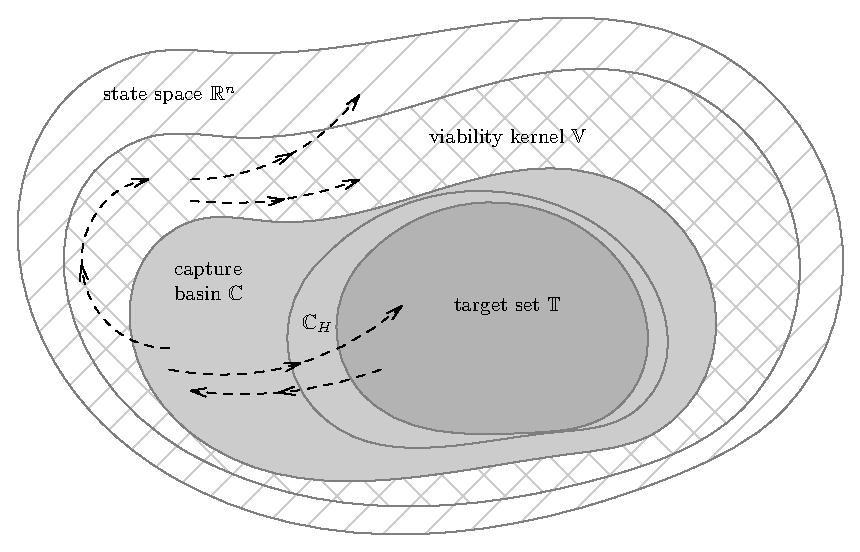
\includegraphics{viability.eps}}
    \caption[Viability kernel, capture basin, and target set.]{
        Viability kernel, capture basin, and target set. Possible evolutions
        are shown with dashed curves.
    }
    \label{fig.viability}
\end{figure}
%


Intuitively, preservation of balance means avoiding \tn{falls} at all future
moments. This definition immediately suggests interpretation using the
viability concepts presented above. Let us assume that we have a set of
constraints, violation of which indicates a fall. Then the balance is ensured
if the state of the robot stays within the viability kernel $\SET{V}$
constructed based on these constraints. In general, it is difficult to check if
a state is inside of the viability kernel, since the computation of $\SET{V}$
appears to be intractable in the case of such complex systems as humanoid
robots \cite{Wieber2002stability}. However, it is usually possible to isolate a
target subset $\SET{T} \subset \SET{V}$ consisting of states, which can be
easily demonstrated to be balanced. For example, $\SET{T}$ may contain states,
in which the robot is stopped, or states comprising a cycle in $\SET{V}$. Later
in this chapter we will see that all common approaches to balance preservation
explicitly or implicitly make use of $\SET{T}$ or the respective capture basin
$\SET{C}$.


Generally speaking, falling is not the only type of a failure, which may happen
to a robot. Depending on the context, failures may be defined as violations of
hardware limits, collisions with the environment, and even undesirable
behaviors, such as bending of the torso while walking. If these failures can
be indicated by some constraints, they can also be described in terms of
viability theory. Therefore, while controlling the robot we should aim at
staying within the viability kernel $\SET{V}$ defined with respect to
constraints reflecting all possible failures. However, in practice it is
usually necessary to consider constraints of different types separately in
sequential schemes for control or planning to tackle the concomitant
computational complexity. In the rest of the thesis the sets $\SET{V}$,
$\SET{C}$, and $\SET{T}$ always take into account the constraints due to
balance preservation and, optionally, other constraints, which are added
depending on the context. Thus, by saying that a particular state is viable or
capturable we imply that a fall can be avoided starting from it.


Though the main control goal is to avoid failures and, in particular, preserve
balance, we argue that this is not sufficient in practice, since we almost
always want the robot to eventually stop, or at least be able to stop. In other
words, the ultimate control goal is not to stay within $\SET{V}$, but rather to
stay within the capture basin $\SET{C}$ corresponding to the target set
$\SET{T}$ composed of the states in which the robot is stopped. This choice of
control goal may appear to be of a philosophical importance due to negligible
difference between the capture basin $\SET{C}$ and viability kernel $\SET{V}$
constructed for some simplified models of humanoid robots
\cite{Zaytsev2015thesis}. However, our point of view has an advantage when it
is necessary to design a controller without explicit knowledge of $\SET{C}$ and
$\SET{V}$: ensuring $\V{x} \in \SET{C}_H$ is easier than $\V{x} \in \SET{V}$.



%%%%%%%%%%%%%%%%%%%%%%%%%%%%%%%%%%%%%%%%%%%%%%%%%%%%%%%%%%%%%%%%%%%%%%%%%%%%%%%%
\subsection{Related terms and concepts}

Legged locomotion is one of the most common tasks of humanoid robots. At the
same time, stepping allows to compensate for perturbations, for example,
pushes. For these reasons, the general problem of balance preservation is often
perceived as a problem of making proper steps. The number of steps required to
stop the robot, and positions of these steps are of particular interest, which
was recognized as early as 70's \cite{Yamashita1974robman}. Consequently,
suitable terminology was introduced in the recent works
\cite{Pratt2006fastmotions, Koolen2012ijrr}, where a certain state is called
$K$-\tn{step capturable}, if the robot can stop by making no more than $K$
steps. Though this term does not originate from viability theory, it does not
contradict with the definition of capturability given above. In particular, the
relation between the capture basin $\SET{C}$ when the target is to stop the
robot and the set of $K$-step capturable states $\SET{K}_K$ is described by
%
\begin{equation}\label{eq.Kcapturability}
    \SET{C} = \bigcup_{K \ge 0} \SET{K}_K.
\end{equation}
%
Some researchers focused on the case, when it is necessary to maintain a
desired walking or running cycle \cite{Carver2009chaos, Zaytsev2015icra}.
Carver studied $K$-\tn{step deadbeat} control laws, which allow to compensate
for disturbances in $K$ steps while running \cite{Carver2009chaos}. Zaytsev
introduced $K$-\tn{step controllability} as generalization of $K$-step
capturability to the cases, when the goal can also be to maintain a given
walking speed \cite{Zaytsev2015thesis}. This case can also be described using
the notion of capturability as defined here: the relation between the set of
$K$-step controllable states and the capture basin is equivalent to
\cref{eq.Kcapturability}.


Viability theory can be applied to many problems in robotics. Hence, it is not
surprising, that some of the application-specific terminology introduced in the
field is equivalent to the notions of viability or capturability. For example,
\tn{inevitable collision states} defined in the context of collision avoidance
comprise the complement of a viability kernel \cite{Fraichard2003iros}. Another
example is the \tn{alternative safe behaviors} constructed in
\cite{Rubrecht2012auro} to avoid violation of the control constraints of a
manipulator. These behaviors are to be triggered to safely stop the robot, when
there is no other way to avoid violation of the constraints. Essentially, this
allows to maintain capturability at all times. Schouwenaars introduced
\tn{terminal feasible invariant sets}, ``\tn{in which a vehicle can remain for
an indefinite period of time without colliding with obstacles or other
vehicles}'', \IE, without violating constraints of the system
\cite[Chapter~4]{Schouwenaars2006thesis}. These sets are conceptually equivalent
to the target sets $\SET{T}$ considered here. Consequently, existence of a
trajectory, which ends in a terminal feasible invariant set, establishes that
the current state of a vehicle is capturable with respect to the system
constraints.


Related concepts are also used in general control theory. For example,
\tn{recursive feasibility} property of \ac{MPC} implies feasibility with
respect to constraints at each future control iteration
\cite[Chapter~8]{Rossiter2003mpc}. Hence, recursive feasibility implies
viability. Some researchers have already pointed out the connection between
viability theory and the notions of \tn{controllability} and \tn{reachability}
\cite{Zaytsev2015icra, Wieber2015handbook} or \tn{control invariant sets}
\cite{Wieber2002stability}. Typically, these notions are employed for simple
cases of linear systems or systems with non-varying constraints
\cite{Sontag1998control, Blanchini2008sets, Borrelli2015mpc,
Kerrigan2000thesis}. As a result, there exists a vast variety of extensions and
specifications meant to adapt controllability, reachability, or control
invariant sets to nonlinear and hybrid systems \cite{Sontag1998control,
Tomlin2003procieee, Bemporad2000tranac, Lewis1999siamr}, to obstacle avoidance
constraints \cite[Chapter~15]{LaValle2006planning} or general varying
constraints \cite[Chapter~2]{Rawlings2009mpc}. We believe that such variety may
lead to a confusion, which can only be resolved by rigorous definitions. For
this reason, here we resort to the concepts of viability theory.



%%%%%%%%%%%%%%%%%%%%%%%%%%%%%%%%%%%%%%%%%%%%%%%%%%%%%%%%%%%%%%%%%%%%%%%%%%%%%%%%
%%%%%%%%%%%%%%%%%%%%%%%%%%%%%%%%%%%%%%%%%%%%%%%%%%%%%%%%%%%%%%%%%%%%%%%%%%%%%%%%
%%%%%%%%%%%%%%%%%%%%%%%%%%%%%%%%%%%%%%%%%%%%%%%%%%%%%%%%%%%%%%%%%%%%%%%%%%%%%%%%
\section{Balance preservation in different settings}

%%%%%%%%%%%%%%%%%%%%%%%%%%%%%%%%%%%%%%%%%%%%%%%%%%%%%%%%%%%%%%%%%%%%%%%%%%%%%%%%
\subsection{Standing}
The states, in which the robot can stay infinitely long without falling, are
called \tn{statically balanced}. A particular state is statically balanced, if
it complies with the hardware limitations and the vertical projection of the
\ac{CoM} of the robot stays within the \tn{support area}, which depends on the
configuration of the contacts with the environment \cite{Wieber2002stability,
Bretl2008tranrob, Santos2005auro}. Though the statically balanced states
\emph{per se} are of little interest for motion control, they can be used to
define the target set $\SET{T}$ and the corresponding capture basin $\SET{C}$.
Such a definition of $\SET{T}$ and $\SET{C}$ is very natural, since we usually
want the robot to stop at some point in the future.


It is common to employ the conditions on the \ac{CoM} for static balance when
the robot is not motionless. The corresponding motions are said to be
\tn{quasi-statically balanced}. This approach is widely used to reject
disturbances while standing or avoid falls while performing simple tasks. One
way to achieve this is to maintain a statically balanced reference
configuration of the body or simply a position of the \ac{CoM}. A less
restrictive alternative is to allow motion of the \ac{CoM} projection within
the support area. Numerous examples of this approach can be found in the
literature using various control methods: standard inverse kinematics
\cite{Escande2014ijrr} or dynamics \cite{Collette2007humanoids},
passivity-based \cite{Hyon2007tro, Ott2011humanoids}, \ac{MPC}
\cite{Henze2014iros}.



%%%%%%%%%%%%%%%%%%%%%%%%%%%%%%%%%%%%%%%%%%%%%%%%%%%%%%%%%%%%%%%%%%%%%%%%%%%%%%%%
\subsection{Regular walk}\label{sec.regular_walk}

One can observe that walking is an intrinsically cyclic process (see
\cref{fig.walkcycle}). Consequently, any balanced regular gait has a
corresponding cycle of states in $\SET{V}$. In order to produce such a gait,
the system has to stay on this cycle comprising the target set $\SET{T}$ and
return to it after perturbations.

%
\begin{figure}[ht]
    \centering{%
    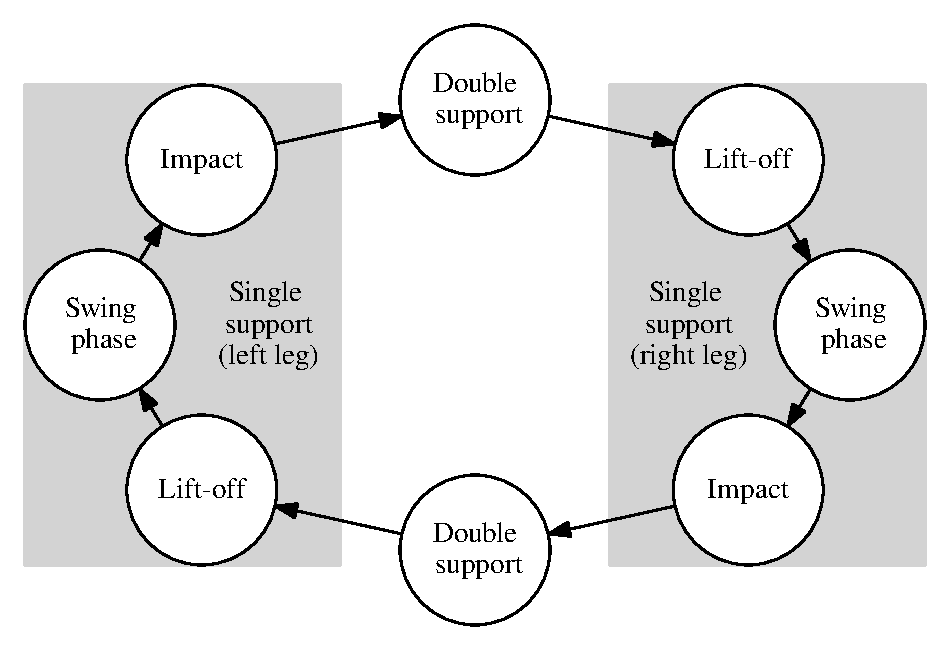
\includegraphics[scale=0.6]{walk_cycle.eps}}
    \caption[Walking cycle of a biped.]{
    Walking cycle of a biped including two \tn{single support} phases, when
    only one foot is on the ground, and two \tn{double support} phases, when
    both feet are on the ground. One single support and one adjacent double
    support comprise a \tn{step}.
    }
    \label{fig.walkcycle}
\end{figure}
%

This goal can be achieved without any actuation by specially designed
mechanical systems called \tn{passive walkers} \cite{McGeer1990ijrs}. They
start walking when positioned on sloped surfaces, where the gravitational force
allows to restore energy lost at foot impacts. Walking on a flat ground can be
enabled by exploiting different sources of energy, for example, heating of the
feet \cite{Nemoto2015iros} or limited actuation \cite{Collins2005science}.
During the walk, the state of passive walkers evolves along a semi-stable limit
cycle $\SET{T}$, whose basin of attraction is the capture basin $\SET{C}$.
Therefore, they can tolerate small perturbations.


The cyclic nature of walking is also exploited in the control of actuated
robots. In particular, the control of a robot as a hybrid system is
significantly simplified due to the sequence of discrete collision events known
in advance. The design and stability analysis of hybrid system controllers is
often further simplified with the help of \tn{virtual constraints} which shape
the walking motion. This approach is referred in the literature as \tn{hybrid
zero dynamics} or \tn{hybrid restriction dynamics} \cite{Westervelt2003tranac,
Chevallereau2003csm, Grizzle2006isccsp, Westervelt2007locomotion}. Typically,
it deals with only planar walking, however, some attempts have been made to
apply it to three dimensional walking as well \cite{Chevallereau2009tro}. Other
researches have also extended this approach to compliant robots
\cite{Sreenath2010ijrr}.


A completely different approach to generation of periodic gaits was inspired by
the neurobiological research. This research indicated a major role of groups of
neurons which generate periodic signals in locomotion of animals. Emulation of
such groups called \tn{central pattern generators} has been successfully
employed in robot locomotion control, even though the balance of the resulting
motion is not usually rigorously proven  \cite{Fukuoka2003ijrr,
Nakanishi2004ras, Ijspeert2008nn}.


The common disadvantage of all these methods is the lack of flexibility: they
are limited to walking and cannot produce acyclic gaits. Sometimes it is also
unclear how to start and terminate the walk or change the walking gait without
falling.



%%%%%%%%%%%%%%%%%%%%%%%%%%%%%%%%%%%%%%%%%%%%%%%%%%%%%%%%%%%%%%%%%%%%%%%%%%%%%%%%
\subsection{General motion and locomotion}\label{sec.balance_general}

Potential practical applications of humanoid robots, such as disaster response
\cite{DRCsite} or airplane assembly \cite{COMANOIDsite}, lie far beyond the
scope of standing or regular walking. Hence, the problem of balance
preservation while performing much more general motions must be addressed. This
is usually achieved as a by-product of motion planning
\cite{LaValle2006planning}, which ensures execution of the motion goals without
falling. We can perceive the motion planning as a procedure of finding a viable
evolution connecting an initial state $\V{x}_s$ and a final state $\V{x}_f \in
\SET{T}$. Whenever $\V{x}_s \notin \SET{C}$ the procedure must necessarily
fail. Note that the sets $\SET{T}$ and $\SET{C}$ are assumed to be defined
based on the constraints taking into account all possible failures.


Determination of a single viable evolution appears to be easier than
determination of the whole $\SET{V}$ and $\SET{C}$ sets. Nevertheless, it is a
very challenging problem, which is usually solved with the help of various
approximations and heuristics. Motion planning in complex situations is often
decoupled into several stages \cite[Chapter~14]{LaValle2006planning}. This
strategy is ubiquitous in planning for legged robots. One of the most commonly
used stages is planning of \tn{stances} -- configurations of the contacts of
the robot with the environment \cite{Bouyarmane2012adrob, Bretl2006ijrr,
Zucker2011ijrr}. Note that, as we have already indicated in
\cref{sec.balance_as_viability}, some of the constraints are neglected on
different stages to reduce computational costs.


An important property of a planning algorithm is \tn{completeness}, \IE, the
ability to find a solution if one exists. In the case of legged robots, it is
common to resort to weaker \tn{probabilistic completeness}
\cite{Kuffner2002auro, Hauser2008ijrr, Dalibard2013ijrr, Shkolnik2011ijrr} or
to \tn{resolution completeness} \cite{Zucker2011ijrr}. The former guarantees
that the probability of finding a solution approaches $1$ as the computation
time increases, the latter is valid for certain resolution of the state space.
Sometimes the completeness is sacrificed by the approaches solely based on
optimization, which may get stuck in a local minimum and, therefore, fail to
find a solution \cite{Dai2014humanoids, Kanoun2010ijrr}.


In spite of an abundance of techniques making motion planning computationally
cheap, it still cannot be performed in real-time. Real-time replanning is,
however, crucial for adaptation to unexpected changes in the environment and
compensation for strong external perturbations \cite{Nishiwaki2009ijrr}. One
way to address this issue is to adjust the precomputed plan if the reality
deviates from it. This may still be intractable in real-time, and a more common
alternative is generation of a short-term plan, which we call motion
\tn{anticipation} or motion \tn{preview}. The performance gain in this case is
achieved due to limited preview horizon, lack of completeness, and, in most
cases, approximated representations of the robot \cite{Kajita2003icra,
Nagasaka2012, Audren2014iros, Nishiwaki2009ijrr}. Low computational cost allows
regeneration of a short-term plan at high frequency, which enables highly
reactive motions. Anticipation can be used to return to the precomputed plan or
can even render it unnecessary for simple motions such as locomotion
\cite{Azevedo2002icra, Wieber2006humanoids, Herdt2010auro, Tassa2014icra,
Sherikov2014humanoids}.


A planned motion is balanced if it complies with all the constraints at all
times and terminates in a final state. The final state, however, usually cannot
be reached, when anticipation over a limited horizon is performed.
Consequently, there is a possibility of reaching a non-viable state. We are not
aware of possibilities to ensure viability without knowledge of the viability
kernel $\SET{V}$. Nevertheless, it is possible to ensure more restrictive
capturability by imposing that the robot must be able to stop or reach certain
walking cycle in the end of preview horizon, \IE, by imposing that the
anticipated motion reaches $\SET{T}$ \cite{Sherikov2014humanoids,
Sherikov2015humanoids, Schouwenaars2006thesis}. Existence of a motion complying
with such constraint implies that the current state $\V{x}_0 \in \SET{C}_H$,
where $H$ is the length of the preview horizon. The requirement to stop does
not undermine the execution of the motion goals provided that two conditions
are met:
%
\begin{enumerate}
    \item the preview horizon is regularly shifted in the future and the
        anticipated motion is recomputed,
    \item the preview horizon is long enough.
\end{enumerate}
%
The first condition implies that the moment, when $\SET{T}$ should be reached,
is continuously postponed. Hence, it is not imposed that the robot stops, but
rather that it maintains the capacity to stop, \IE, capturability. The second
condition is also straightforward: if the robot is required to reach $\SET{T}$
the very next moment, it hardly has enough freedom to execute the motion goals.
This naturally leads to the question about sufficient length of the preview
horizon. Currently, we do not have an answer for the general case: the choice
may well be application dependent. However, the existing research on walking of
both humans and robots strongly suggests that the length of a preview horizon
should cover $2$ or $3$ steps \cite{Zaytsev2015icra, Carver2009chaos,
Kajita2003icra, Koolen2012ijrr, Sparrow2005gaitpost, Vukobratovic1970tranbme}.


The idea of maintaining capturability by imposing that $\SET{T}$ is reached at
the end of a preview horizon is recurrent in the literature. Implementation,
however, is dependent on the particular method chosen for anticipation: the
motion may be a result of solution of a boundary value problem, or an \ac{MPC}
problem with terminal constraints \cite{Mansour2011humanoids, Henze2014iros,
Sherikov2014humanoids, Morisawa2007icra, Takenaka2009iros}. The target set
$\SET{T}$ is usually defined so that the robot's ability to stop
\cite{Mansour2011humanoids, Henze2014iros} is ensured or cyclicity of motions
is enforced \cite{Takenaka2009iros}.




%%%%%%%%%%%%%%%%%%%%%%%%%%%%%%%%%%%%%%%%%%%%%%%%%%%%%%%%%%%%%%%%%%%%%%%%%%%%%%%%
%%%%%%%%%%%%%%%%%%%%%%%%%%%%%%%%%%%%%%%%%%%%%%%%%%%%%%%%%%%%%%%%%%%%%%%%%%%%%%%%
%%%%%%%%%%%%%%%%%%%%%%%%%%%%%%%%%%%%%%%%%%%%%%%%%%%%%%%%%%%%%%%%%%%%%%%%%%%%%%%%
\section{Conclusion}\label{sec.conclusion}

We have defined the balance preservation problem using notions of viability
theory and briefly reviewed existing approaches to this problem based on our
definition. Henceforth, we are going to focus on online control and balancing
of humanoid robots performing general motions. We assume that a global motion
plan is not provided or only partial information, such as planned contact
positions, is given. Therefore, we completely rely on motion anticipation with
limited preview horizon. In the preceding section it is indicated, that
capturability can be enforced in such a situation by imposing appropriate
conditions on the final previewed state. Commonly, these conditions ensure the
capacity of the robot to stop or maintain a cyclic motion. We believe the first
option to be more appropriate, since it allows for generation of both cyclic
and acyclic motions. Hence, in the following chapters we narrow the notion of
capturability by assuming that it implies the capacity of the robot to reach a
statically balanced state, \IE, to stop.

%-------------------------------------------------------------------------------
\chapter{Modeling of a humanoid robot}
\label{ch.modeling}
\acresetall
%-------------------------------------------------------------------------------

A very abstract model of a humanoid robot~\cref{eq.general_system} was
sufficient for the discussion in \cref{ch.balance}, but it is of no use for
practical applications. Therefore, in the present chapter we specify and study
the structure of humanoid robot models. Though we employ only the whole body
model for control (\cref{sec.whole_body_model}) and approximate linear models
for anticipation (\cref{sec.linear_approx_models}), we also consider
approximate nonlinear models in \cref{sec.nonlinear_approx_models} to
demonstrate the ancestral relationships between these models. These
relationships can be illustrated with the following tree

\begin{forest}
  for tree={
    grow'=0,
    child anchor=west,
    parent anchor=south,
    anchor=west,
    calign=first,
    edge path={
      \noexpand\path [draw, \forestoption{edge}]
      (!u.south west) +(7.5pt,0) |- node[fill,inner sep=1.25pt] {} (.child anchor)\forestoption{edge label};
    },
    before typesetting nodes={
      if n=1
        {insert before={[,phantom]}}
        {}
    },
    fit=band,
    before computing xy={l=25pt},
  }
[Whole body (\nameref{model.WB}) model (\cref{sec.whole_body_model})
    [Nonlinear momenta-based (\nameref{model.NMB}) model (\cref{sec.momenta_based_nonlinear})
        [Nonlinear point-mass (\nameref{model.NPM}) model (\cref{sec.point_mass_nonlinear})
            [\begin{minipage}{11cm}Linear point-mass models (\nameref{model.CPPMJ} and \nameref{model.CPPMdZ}) with planar \ac{CoM} motion (\cref{sec.point_mass_planar})\end{minipage}]
            [\begin{minipage}{11cm}Linear point-mass model (\nameref{model.CNPM}) with nonplanar \ac{CoM} motion (\cref{sec.point_mass_nonplanar})\end{minipage}]
        ]
    [Linear momenta-based (\nameref{model.CMB}) model (\cref{sec.model_momenta})]
  ]
]
\end{forest}


We present detailed derivations of the models and try to be explicit about all
assumptions made in the process. Most of the assumptions are introduced to
linearize models in order to fit them in the \ac{PLLS} framework
(\cref{ch.optimization}), which we employ for both control and anticipation.



%%%%%%%%%%%%%%%%%%%%%%%%%%%%%%%%%%%%%%%%%%%%%%%%%%%%%%%%%%%%%%%%%%%%%%%%%%%%%%%%
%%%%%%%%%%%%%%%%%%%%%%%%%%%%%%%%%%%%%%%%%%%%%%%%%%%%%%%%%%%%%%%%%%%%%%%%%%%%%%%%
%%%%%%%%%%%%%%%%%%%%%%%%%%%%%%%%%%%%%%%%%%%%%%%%%%%%%%%%%%%%%%%%%%%%%%%%%%%%%%%%
\section{Whole body dynamical model}\label{sec.whole_body_model}

We start by considering the whole body model of a humanoid robot. A humanoid
robot is a chain of $n+1$ links interconnected by $n$ joints. In general,
joints can be rotary or prismatic, actuated or not actuated. While all these
joint types can be incorporated in the model without much effort, we limit our
discussion to actuated rotary joints only, since the other types are rare in
humanoid robots. The links composing the robot can be in contact with the
environment, but are not fixed to any support. Therefore, the robot must be
modeled taking contacts and contact friction into account. We use \tn{Coulomb's
law} as a friction model \cite[Chapter~10]{Popov2010contact} and make the
following additional assumptions:
%
\begin{description}
    \item[\ass{ass.frictioncoef}] coefficients of static and kinetic (dynamic)
        friction are equal and constant \cite[Chapter~10]{Popov2010contact};
    \item[\ass{ass.norolling}] there are no rolling contacts;
    \item[\ass{ass.rigid}] the environment and links of the robot are rigid;
    \item[\ass{ass.fixed_environment}] the robot contacts only the objects,
        whose positions are fixed in the environment;
    \item[\ass{ass.nojointfriction}] there is no friction in the joints;
    \item[\ass{ass.nouncertainty}] there are no noises in measurements of the
        state and no inaccuracies in parameters of the robot.
\end{description}
%
\cref{ass.frictioncoef} is ubiquitous in the literature.
\cref{ass.norolling,ass.rigid,ass.fixed_environment} are not valid in some
settings, but we do not consider such settings and thus avoid the burden of
more accurate modeling. The last two assumptions can never be fulfilled in
practice. However, friction in the joints can be modeled, if the corresponding
parameters of the robot are provided, or it can be concealed by joint-level
position controllers of a robot such as \sn{HRP-2} \cite{Kaneko2004icra}. The
problem of uncertainty, on the other hand, is not addressed by modeling, but
rather by robust control and techniques for estimation of parameters and state
\cite[Chapter~8]{Siciliano2010robotics}, \cite{Christensen2008handbook}. We
leave such topics outside of the scope of this thesis.


Based on the listed assumptions, we present the whole body model in the
following \cref{sec.complementarity_system}.
\cref{sec.wbm_constraints,sec.contact_constraints} focus on constraints
included in the model and their linearization. \cref{sec.linear_wbm} presents a
whole body model with linear constraints, while concluding
\cref{sec.wbm_control} overviews the control of the robot using this model.



%%%%%%%%%%%%%%%%%%%%%%%%%%%%%%%%%%%%%%%%%%%%%%%%%%%%%%%%%%%%%%%%%%%%%%%%%%%%%%%%
\subsection{Humanoid robot as a complementarity system}\label{sec.complementarity_system}

Under \crefrange{ass.frictioncoef}{ass.nouncertainty} the humanoid robot is
described by a \tn{complementarity system} \cite{Brogliato2003tranac,
Hurmuzlu2004automatica}, whose form at a given time instant with $M$ contacts
is \cite{Trinkle1997zamm}
%
\begin{subequations}\label{eq.complementarity_system}
\begin{empheq}[left=\empheqlbrace]{align}
    & \M{H}(\q) \ddq + \V{h}(\q, \dq) = \Itorques\torques + m\T{\Jcom}(\q) \V{g} + \T{\Jcontact}(\q) \allcontactf,
      \label{eq.complementarity_system.dynamics}\\[2mm]
    & \ubarV{\objb} \le \FUNC{A} (\ddq, \dq, \q, \torques) \le \barV{\objb},
      \label{eq.complementarity_system.constraints}\\[2mm]
    & \ddcontactC^n_i \ge 0,
      \label{eq.complementarity_system.nonpenetration}\\
    & \forceC_i^n \ge 0,
      \label{eq.complementarity_system.unilaterality}\\
    & \ddcontactC^n_i \forceC_i^n = 0,
      \label{eq.complementarity_system.complementarity}\\[2mm]
    & \friction_i^2 (\forceC_i^n)^2 - \T{(\force_i^t)} \force_i^t \ge 0,
      \label{eq.complementarity_system.frictioncone}\\
    %|| n x f x n || =< \friction(f^T n)
    & \friction_i \forceC_i^n \dcontact^t_i - \force_i^t \NORME{\dcontact^t_i} = 0,
      \label{eq.complementarity_system.frictiondirection}
\end{empheq}
\end{subequations}
%
where $i \in \{1, ..., M\}$,
%
\begin{subequations}
    \begin{align}
        & (\ddcontact_1, \dots, \ddcontact_M) = \Jcontact(\q) \ddq + \dJcontact(\q) \dq, \\
        & (\force_1, ..., \force_M) = \allcontactf,
    \end{align}
\end{subequations}
%
and variables have the following meaning
%
\begin{longtable}[l]{@{\extracolsep{0pt}}l @{\extracolsep{3pt}}l p{9.5cm}}
    $\q = (\qn, \V{r}, \V{\EULER})$         & $\in \RR^{n+3+3}$              & vector of generalized coordinates including
                                                                               $n$ joint angles $\qn$, position of the base $\V{r}$,
                                                                               and orientation of the base represented with Euler angles $\V{\EULER}$\\
    $\torques$                              & $\in \RR^n$                    & vector of joint torques\\
    $\force_i$                              & $\in \RR^{3}$                  & $i$-th contact force\\
    $\contact_i$                            & $\in \RR^{3}$                  & position of the $i$-th contact \\
    $\M{H}(\q)$                             & $\in \RR^{(n+6) \CROSS (n+6)}$ & inertia matrix\\
    $\V{h}(\q, \dq)$                        & $\in \RR^{n+6}$                & vector of Coriolis and centrifugal terms\\
    $\Jcom$                                 & $\in \RR^{3 \CROSS (n+6)}$     & Jacobian of the \ac{CoM} (see \cref{sec.momenta_structure})\\
    $\Jcontact$                             & $\in \RR^{3M \CROSS (n+6)}$    & translational Jacobian of the contact points\\
    $\Itorques = (\M{I}_n, \M{0}_{6,n})$    & $\in \RR^{(n+6) \CROSS n}$     & torque selection matrix\\
    $\V{g}$                                 & $\in \RR^3$                    & vector of gravitational acceleration\\
    $\friction_i$                           & $\in \RR_{\ge 0}$              & friction coefficient of the $i$-th contact\\
    $m$                                     & $\in \RR_{>0}$                 & total mass of the system\\
    $\FUNC{A}, \ubarV{\objb},\barV{\objb}$  &                                & function, which expresses application dependent
                                                                               constraints on the state and controls, and its bounds\\
\end{longtable}
%
\noindent Superscripts $(\cdot)^t$ and $(\cdot)^n$ denote tangential and normal
components of vectors with respect to the contact surfaces as shown in
\cref{fig.friction_cone_contact}. These components are obtained by expressing
vectors in local frames $\FRAME{i}$ using rotation matrices $\M[][i]{R}$:
%
\begin{equation}
    \begin{bmatrix}
        \ddcontact^{t}_i\\
        \ddcontactC^{n}_i
    \end{bmatrix}
    =
    \M[][i]{R}
    \ddcontact_i,
    \enspace
    \begin{bmatrix}
        \dcontact^{t}_i\\
        \dcontactC^{n}_i
    \end{bmatrix}
    =
    \M[][i]{R}
    \dcontact_i,
    \enspace
    \begin{bmatrix}
        \force^{t}_i \\
        \forceC^{n}_i
    \end{bmatrix}
    =
    \M[][i]{R}
    \force_i
    .
\end{equation}
%
Each frame $\FRAME{i}$ is fixed to the contact point and its $z$ axis is normal
to the contact surface.


%
\begin{figure}
    \centering{%
    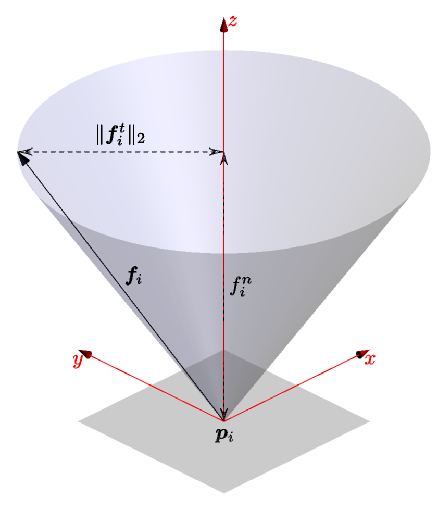
\includegraphics{friction_cone_contact.eps}}
    \caption[Friction cone and the local frame $\FRAME{i}$ of the $i$-th contact.]{
        Friction cone and the local frame $\FRAME{i}$ of the $i$-th contact.
        Square patch indicates the contact surface.
    }
    \label{fig.friction_cone_contact}
\end{figure}
%

Individual components of system~\cref{eq.complementarity_system} have the
following interpretation
\begin{description}
    \item[\cref{eq.complementarity_system.dynamics}] is the standard equation
        of dynamics of a multibody system (see \cref{app.dynamics}). The
        equation establishes relationship between motion of the joints and
        forces acting on the robot.

    \item[\cref{eq.complementarity_system.constraints}] represents constraints
        of a particular robot and setting, for example, mechanical constraints.
        These constraints are discussed later in \cref{sec.wbm_constraints}.

    \item[\cref{eq.complementarity_system.nonpenetration}] prevents
        interpenetration of the contact surface and the contacting body.

    \item[\cref{eq.complementarity_system.unilaterality}] indicates that the
        contacts are unilateral, \IE, the robot can push on the contact
        surface, but cannot pull on it.

    \item[\cref{eq.complementarity_system.complementarity}] is the
        complementarity condition, which states that a contact force cannot be
        applied at a contact surface if the contact point detaches from this
        surface.

    \item[\cref{eq.complementarity_system.frictioncone}] bounds tangential
        components of the contact force depending on the norm of its normal
        component in accordance with Coulomb's friction law.

    \item[\cref{eq.complementarity_system.frictiondirection}] indicates that
        the tangential component of the contact force is opposite to the
        sliding velocity of the contact point.
\end{description}


In order to complete the model we have to consider one more important aspect,
which manifests itself in the discrete nature of changes of the set of
contacts. These changes, or \tn{switches} of the mode of the system, indicate
that the system at hand is \tn{hybrid}. The state of such a system is often
discontinuous at the instant of a switch, and a \tn{state reinitialization
rule} must be defined \cite{Brogliato2003tranac}. In the case of the considered
system with contacts we employ an \tn{impact law} described in
\cref{app.collision} as a reinitialization rule.


%%%%%%%%%%%%%%%%%%%%%%%%%%%%%%%%%%%%%%%%%%%%%%%%%%%%%%%%%%%%%%%%%%%%%%%%%%%%%%%%
\subsection{Mechanical constraints}\label{sec.wbm_constraints}

The general inequality \cref{eq.complementarity_system.constraints} comprises
mechanical limits of the joints and motors
%
\begin{subequations}\label{eq.mechanical_constraints}
\begin{align}
    \ubar{\q}^{\prime}
    \le
    \qn
    \le
    \bar{\q}^{\prime},
    \quad
    \ubar{\dq}^{\prime}
    \le
    &
    \dqn
    \le
    \bar{\dq}^{\prime},
    \quad
    \ubar{\ddq}^{\prime}
    \le
    \ddqn
    \le
    \bar{\ddq}^{\prime}, \label{eq.joint_constraints}\\
    \ubar{\torques}
    \le
    &
    \torques
    \le
    \bar{\torques}.
\end{align}
\end{subequations}
%
In general, constraints \cref{eq.complementarity_system.constraints} are not
limited to \cref{eq.mechanical_constraints}, but such cases are not considered
in this work.


Enforcement of constraints \cref{eq.joint_constraints} is not straightforward,
when the model is used exclusively for instantaneous control. In this case, the
current state $(\q, \dq)$ is given and cannot be constrained, while the next
state is not explicitly computed. For this reason, constraints on the joint
angles and velocities are imposed through the joint accelerations. Hence,
\cref{eq.joint_constraints} boils down to \cite{Rubrecht2012auro}
%
\begin{equation}
    \ubar{\ddq}^{\prime}(\qn,\dqn)
    \le
    \ddqn
    \le
    \bar{\ddq}^{\prime}(\qn,\dqn),
\end{equation}
%
where bounds on accelerations incorporate bounds on joint angles and velocities
as well. We discuss computation of $\ubar{\ddq}^{\prime}(\qn,\dqn)$ and
$\bar{\ddq}^{\prime}(\qn,\dqn)$ in \cref{app.jointconstraints}.


%%%%%%%%%%%%%%%%%%%%%%%%%%%%%%%%%%%%%%%%%%%%%%%%%%%%%%%%%%%%%%%%%%%%%%%%%%%%%%%%
\subsection{Contact constraints and assumptions}\label{sec.contact_constraints}

One of the primary sources of nonlinearity of system
\cref{eq.complementarity_system} are the contact constraints. In order to
linearize them we make a number of approximations and assumptions. We start by
assuming that
%
\begin{description}
    \item[\ass{ass.nosliding}] There is no sliding, \IE, $\NORME{\dcontact^t_i}
        = 0$. In order to enforce this,
        constraint~\cref{eq.complementarity_system.frictiondirection}, which is
        not needed now, is replaced with
        %
        \begin{equation}\label{eq.no_tangential_acc}
            \ddcontact^t_i = \V{0}.
        \end{equation}
        %
        While being useful in manipulation~\cite{Howe1996ijrr} sliding is less
        common in locomotion~\cite{Miura2013tro}, and is usually prevented to
        simplify control.

    \item[\ass{ass.no_break_contacts}] Contacting bodies do not detach, and,
        consequently, constraint
        %
        \begin{equation}\label{eq.no_normal_acc}
            \ddcontactC^n_i = 0
        \end{equation}
        %
        must be imposed instead of nonpenetration constraint
        \cref{eq.complementarity_system.nonpenetration} and complementarity
        condition \cref{eq.complementarity_system.complementarity}. This is
        also a typical assumption. Whenever it is necessary to break one of the
        contacts, constraint \cref{eq.no_normal_acc} is replaced by a motion
        task for the contacting body.
\end{description}
%

\begin{figure}[ht]
    \begin{minipage}[t]{0.45\textwidth}
        \centering{%
        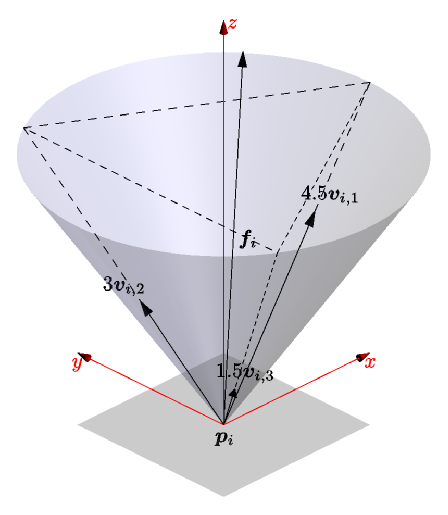
\includegraphics{friction_cone3.eps}}
        \subcaption{
            Friction cone. The force vector is represented by a weighted sum of
            vectors: $\force_i = 4.5\genvector_{i,1} + 3\genvector_{i,2} +
            1.5\genvector_{i,3}$.
        }
        \label{fig.friction_cone3}
    \end{minipage}
    \hfill
    \begin{minipage}[t]{0.45\textwidth}
        \centering{%
        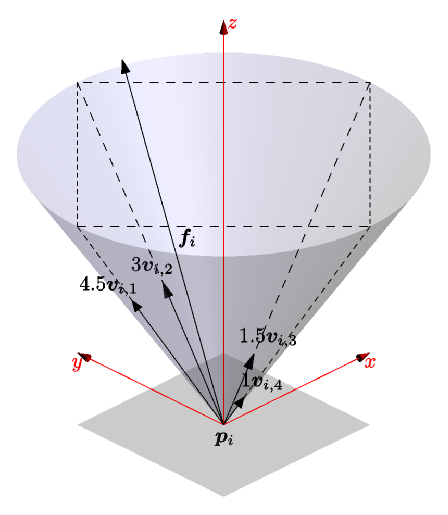
\includegraphics{friction_cone4.eps}}
        \subcaption{
            Friction cone. The force vector is represented by a weighted sum of
            vectors: $\force_i = 4.5\genvector_{i,1} + 3\genvector_{i,2} +
            1.5\genvector_{i,3} + \genvector_{i,4}$.
        }
        \label{fig.friction_cone4}
    \end{minipage}
    \caption{Linear approximation of a friction cone.}
    \label{fig.friction_cone}
\end{figure}

The next step is to linearize the quadratic
constraint~\cref{eq.complementarity_system.frictioncone}, which bounds the
$i$-th tangential contact force with respect to the normal contact force in
accordance with Coulomb's friction law. In order to linearize it, we replace
the second order cones with pyramids as shown in \cref{fig.friction_cone}. Then
for a pyramid with three faces (\cref{fig.friction_cone3}) the constraint is
expressed as
%
\begin{equation}\label{eq.friction_approx1}
    \begin{bmatrix}
        \T{(\genvector_{i,1} \CROSS \genvector_{i,2})} \\
        \T{(\genvector_{i,2} \CROSS \genvector_{i,3})} \\
        \T{(\genvector_{i,3} \CROSS \genvector_{i,1})} \\
    \end{bmatrix}
    \force_i
    \ge
    \V{0}
    ,
\end{equation}
%
where $\V{v}_{i,\{1, 2, 3\}}$ are unity vectors coinciding with the edges of
the pyramid, and cross product is used to obtain normals of the faces. Note
that \cref{eq.friction_approx1} implies unilaterality constraint
\cref{eq.complementarity_system.unilaterality} $\forceC_i^n \ge 0$, which
becomes redundant and should be removed from the system. There exist several
approaches to representation of the linearized constraints
\cite{Kuindersma2014icra}, and the one used in \cref{eq.friction_approx1} is
not optimal when it comes to solution of the system of constraints. We perform
a change of variables to express these constraints as simple bounds, which are
beneficial for solvers as indicated in \cref{sec.simple_bounds}:
%
\begin{equation}\label{eq.friction_approx2}
    \force_i
    =
    \begin{bmatrix}
        \genvector_{i,1} & \genvector_{i,2} & \genvector_{i,3}
    \end{bmatrix}
    \V{\lambda}_i
    =
    \M{V}_i
    \V{\lambda}_i,
    \quad
    \V{\lambda}_i \ge \V{0}.
\end{equation}
%


Accuracy of the linear approximation increases with the number of faces of
pyramids, which is typically chosen to be 3 or 4
(\cref{fig.friction_cone3,fig.friction_cone4} respectively). We use pyramids
with three faces, because it results in the least number of inequality
constraints.


The number of inequality constraints is further reduced by representing a foot
contact force by a single wrench $\wrench_i = (\force_i, \moment_i) =
(\M{V}_i\V{\lambda}_i, \moment_i)$ applied at $\contact_i$ instead of multiple
$3$-dimensional forces applied at several points on the foot. The force
component of the wrench is subject to Coulomb's friction constraint as above,
while the moment is constrained by
%
\begin{equation}\label{eq.moment_constraint}
    \forceC^n_i \ubar{\moment}_i \le \moment[i]_i \le  \forceC^n_i \bar{\moment}_i
    ,
    \quad
    \mbox{or}
    \quad
    \forceC^n_i \ubar{\moment}_i \le \M[][i]{R} \moment_i \le  \forceC^n_i \bar{\moment}_i
\end{equation}
%
where $\ubar{\moment}_i$ and $\bar{\moment}_i$ are constant vectors derived in
\cref{sec.rectangular_foot}, $\M[][i]{R}$ transforms the moment to the local
frame of $i$-th contact. This constraint is linear with respect to
$\V{\lambda}_i$ and $\moment_i$ and in the following is stated as
%
\begin{equation}\label{eq.moment_constraint2}
    \objA_{\moment,i}
    \begin{bmatrix}
        \V{\lambda}_i\\
        \moment_i
    \end{bmatrix}
    \ge
    \ubarV{\objb}_{\moment,i}.
\end{equation}
%


When a foot contact is represented by three or
more contact points, the orientation of the foot is fixed. In order to prevent
rotation of the foot, when the foot contact is represented by a single point
$\contact_i$, it is necessary to fix angular acceleration with the constraint
%
\begin{equation}\label{eq.no_contact_rotation}
    \dcontactW_i = \JcontactWi \ddq + \dJcontactWi \dq = \V{0}.
\end{equation}
%


%%%%%%%%%%%%%%%%%%%%%%%%%%%%%%%%%%%%%%%%%%%%%%%%%%%%%%%%%%%%%%%%%%%%%%%%%%%%%%%%
\subsection{Whole body model with linear constraints}\label{sec.linear_wbm}

Substitution of the constraints obtained in
\cref{sec.wbm_constraints,sec.contact_constraints} into the complementarity
system \cref{eq.complementarity_system} results in the whole body model with
linear constraints
%
\begin{model}{WB}{Whole Body}
\begin{subequations}\label{eq.linearized_system}
\begin{empheq}[left=\empheqlbrace]{align}
    & \M{H} \ddq + \V{h} = \Itorques\torques + m\T{\Jcom} \V{g} + \sum_{i=1}^M \T{\M{J}_i} \wrench_i
        ,
        \\
    &
        \begin{bmatrix}
            \ddcontact_i \\
            \dcontactW_i
        \end{bmatrix}
        =
        \begin{bmatrix}
            \Jcontacti \\
            \JcontactWi
        \end{bmatrix}
        \ddq
        +
        \begin{bmatrix}
            \dJcontacti \dq \\
            \dJcontactWi \dq
        \end{bmatrix}
        =
        \M{J}_i
        \ddq
        +
        \dotM{J}_i
        \dq
        =
        \V{0}
        ,
        \label{eq.linearized_system.fixedcontact}
        \\
    & \ubar{\torques}  \le  \torques  \le  \bar{\torques}
        ,
        \label{eq.linearized_system.ctrtorques}
        \\
    & \ubar{\ddq}^{\prime}  \le  \ddqn  \le  \bar{\ddq}^{\prime}
        ,
        \label{eq.linearized_system.ctrq}
        \\
    &
        \objA_{\moment,i}
        \begin{bmatrix}
            \V{\lambda}_i\\
            \moment_i
        \end{bmatrix}
        \ge
        \ubarV{\objb}_{\moment,i}
        \label{eq.linearized_system.moments}
        ,
        \\
    &
        \V{\lambda}_i \ge \V{0}
        ,
        \label{eq.linearized_system.friction}
\end{empheq}
\end{subequations}
\end{model}
%
where $\wrench_i = (\force_i, \moment_i) = (\M{V}_i\V{\lambda}_i, \moment_i)$,
$\M{J}_i$ is the contact point Jacobian including both translational and
rotational parts. Dependence of $\M{H}$, $\V{h}$, $\ubar{\ddq}^{\prime}$,
$\bar{\ddq}^{\prime}$, and Jacobians on $\q$ and $\dq$ is omitted for brevity.
Equation \cref{eq.linearized_system.fixedcontact} incorporates constraints
\cref{eq.no_tangential_acc}, \cref{eq.no_normal_acc}, and
\cref{eq.no_contact_rotation}.



%%%%%%%%%%%%%%%%%%%%%%%%%%%%%%%%%%%%%%%%%%%%%%%%%%%%%%%%%%%%%%%%%%%%%%%%%%%%%%%%
\subsection{Controlling the robot}\label{sec.wbm_control}

The primary interest of our modeling effort is to allow control of a humanoid
robot using its model. It turns out, that we have already introduced elements
of control in \nameref{model.WB} model by adding constraint
%
\begin{equation}\label{eq.fixed_position}
    \ddcontact_i = \Jcontacti \ddq + \dJcontacti \dq = \V{0}
\end{equation}
%
in order to support \cref{ass.nosliding,ass.no_break_contacts}. This constraint
is clearly not physical, but rather dictated by our control goals. It falls
within the framework of \tn{operational space control} \cite{Khatib1987jra} or
more general \tn{task function control approach}
\cite[Chapter~3]{Samson1991robot}, both of which focus on control of the
end-effectors of the robot rather than its joints. Hence, we call
\cref{eq.fixed_position} a \tn{task}, whose purpose is to maintain constant
position of the end-effector corresponding to the contact point. In a similar
way we define tasks for other parts of the robot's body
%
\begin{equation}
    \M{J}_{\!\MT{ee}}\ddq + \dotM{J}_{\!\MT{ee}} \dq = \ddotV{y}^{\DES}_{\!\MT{ee}},
\end{equation}
%
where $\M{J}_{\!\MT{ee}}$ and $\ddotV{y}^{\DES}_{\!\MT{ee}}$ are the Jacobian
and the desired acceleration of a certain end-effector.
$\ddotV{y}^{\DES}_{\!\MT{ee}}$ can be obtained with a simple
\acs{PD}-controller such as
%
\begin{equation}
    \ddotV{y}^{\DES}_{\!\MT{ee}}
    =
    \K_{p,\MT{ee}} (\V{y}^{\DES}_{\!\MT{ee}} - \V{y}_{\!\MT{ee}})
    -
    \K_{d,\MT{ee}} \dotV{y}_{\!\MT{ee}},
\end{equation}
%
which drives the end-effector to the desired position
$\V{y}^{\DES}_{\!\MT{ee}}$ given current position $\V{y}$ and velocity
$\dotV{y}$, and positive scalar gains $\K_{p,\MT{ee}}$, $\K_{d,\MT{ee}}$.
Examples of various end-effector tasks for humanoid robots can be found in
\cite[Chapter~4]{Kanoun2009thesis}.


Tasks, however, are not limited to control of the end-effectors. For example,
the joint-level task
%
\begin{equation}
    \ddqn = \K_{p,\qn} (\qn[\DES] - \qn) - \K_{d,\qn} \dqn
\end{equation}
%
employs a \acs{PD}-controller to maintain the desired joint configuration
$\qn[\DES]$. Furthermore, tasks can also be posed as inequalities
\cite[Chapter~3]{Kanoun2009thesis}
%
\begin{equation}
    \ubar{\ddotV{y}}_{\!\MT{ee}}
    \le
    \M{J}_{\!\MT{ee}}\ddq + \dotM{J}_{\!\MT{ee}} \dq
    \le
    \bar{\ddotV{y}}_{\!\MT{ee}}.
\end{equation}
%
Thus, we conclude that the difference between tasks and constraints in the
model is only a matter of interpretation: as we are going to see in
\cref{ch.optimization}, the only important thing for numerical computations is
prioritization of the constraints or tasks with respect to each other. Hence,
in the following we use terms ``task'' and ``constraint'' interchangeably.


All whole body motion controllers employed in this work include tasks for
control of motion of the \ac{CoM} and orientation of the body, which are
related to linear and angular momenta respectively. Both are important for
balance preservation: in order to stop the robot it is necessary to nullify its
momenta. Furthermore, control over vertical motion of the \ac{CoM} helps to
prevent falls, which cannot be prevented by the constraints in
\nameref{model.WB} model. The desired values for momenta are obtained by
anticipating the motion of the robot with approximate linear models described
later in this chapter.


While controlling the robot using the task function approach, we may encounter
several types of problems. The first problem arises when imposed tasks do not
require all degrees of freedom of the system. This implies that the robot is
\tn{redundant} with respect to the tasks and there is an infinite number of
control inputs that achieve our goals \cite[Chapter~4]{Samson1991robot}. We can
easily alleviate this issue by adding tasks, which, however, increase the
chance of triggering the second problem: a \tn{conflict} of the tasks with each
other and the physical constraints. Both redundancy and conflicts are important
subjects of this thesis and are discussed in \cref{ch.optimization}. Another
important question is dealing with online addition, removal, or transformation
of the tasks, which is not considered here \cite{Lee2012tro}.



%%%%%%%%%%%%%%%%%%%%%%%%%%%%%%%%%%%%%%%%%%%%%%%%%%%%%%%%%%%%%%%%%%%%%%%%%%%%%%%%
%%%%%%%%%%%%%%%%%%%%%%%%%%%%%%%%%%%%%%%%%%%%%%%%%%%%%%%%%%%%%%%%%%%%%%%%%%%%%%%%
%%%%%%%%%%%%%%%%%%%%%%%%%%%%%%%%%%%%%%%%%%%%%%%%%%%%%%%%%%%%%%%%%%%%%%%%%%%%%%%%
\section{Nonlinear approximate models}\label{sec.nonlinear_approx_models}

The whole body (\nameref{model.WB}) model reviewed in
\cref{sec.whole_body_model} allows for the control of the robot, but it varies
nonlinearly with the state of the system and is rather complicated. We have
already indicated in \cref{sec.balance_general}, that such complexity is not
always needed when online motion anticipation is performed. In this case it is
common to employ approximate models, which are derived from the complete model
under certain assumptions. In the present section we consider two approximate
nonlinear models, which we do not employ \tn{per se}, but use them later in
\cref{sec.linear_approx_models} for the construction of linear models.


%%%%%%%%%%%%%%%%%%%%%%%%%%%%%%%%%%%%%%%%%%%%%%%%%%%%%%%%%%%%%%%%%%%%%%%%%%%%%%%%
\subsection{Nonlinear momenta-based model}\label{sec.momenta_based_nonlinear}

First, let us consider the friction constraints
\cref{eq.linearized_system.moments}, \cref{eq.linearized_system.friction} in
\nameref{model.WB} model. It is interesting to observe that they primarily
limit the aggregate motion of the robot, \IE, the rate of its spatial momentum.
That is, as long as the rate of momentum complies with these constraints, the
joint motion can be arbitrary, provided that the motors can produce sufficient
torques and joint limits are satisfied. We demonstrate this by rewriting the
equation of dynamics using derivations from \cref{app.dynamics} as
%
\begin{equation}
    \underbrace{
        \begin{bmatrix}
            \M{H}_1\\
            \M{H}_2\\
            \M{H}_3\\
        \end{bmatrix}
    }_{\M{H}}
    \underbrace{
        \begin{bmatrix}
            \ddqn\\
            \ddotV{r}\\
            \ddotV{\EULER}
        \end{bmatrix}
    }_{\ddq}
    +
    \underbrace{
        \begin{bmatrix}
            \V{h}_1\\
            \V{h}_2\\
            \V{h}_3
        \end{bmatrix}
    }_{\V{h}}
    =
    \begin{bmatrix}
        \torques\\
        \V{0}\\
        \V{0}
    \end{bmatrix}
    +
    m
    \underbrace{
        \begin{bmatrix}
            \T{\Jcom[,1]}\\
            \T{\Jcom[,2]}\\
            \T{\Jcom[,3]}
        \end{bmatrix}
    }_{\T{\Jcom}}
    \V{g}
    +
    \sum_{i=1}^M
    \underbrace{
        \begin{bmatrix}
            \T{\M{J}_{i,1}}\\
            \T{\M{J}_{i,2}}\\
            \T{\M{J}_{i,3}}
        \end{bmatrix}
    }_{\T{{\M{J}}_i}}
    \wrench_i,
\end{equation}
%
and use the first line of this equation to eliminate $\torques$ from
\nameref{model.WB} model to obtain
%
\begin{subequations}\label{eq.eliminated_torques}
\begin{empheq}[left=\empheqlbrace]{align}
    &   \begin{bmatrix}
            \M{I}   &   \M{0} \\
            \M{0}   &   \T{\Teuler}\\
        \end{bmatrix}
        \begin{bmatrix}
            \dotV[r]{\LM} \\
            \dotV[r]{\AM}\\
        \end{bmatrix}
        =
        \begin{bmatrix}
            \M{H}_2\\
            \M{H}_3\\
        \end{bmatrix}
        \ddq
        +
        \begin{bmatrix}
            \V{h}_2\\
            \V{h}_3
        \end{bmatrix}
        =
        m
        \begin{bmatrix}
            \T{\Jcom[,2]}\\
            \T{\Jcom[,3]}
        \end{bmatrix}
        \V{g}
        +
        \sum_{i=1}^M
            \begin{bmatrix}
                \T{\M{J}_{i,2}}\\
                \T{\M{J}_{i,3}}
            \end{bmatrix}
        \begin{bmatrix}
            \force_i\\
            \moment_i
        \end{bmatrix},
        ,
        \\
    &   \begin{bmatrix}
            \ddcontact_i \\
            \dcontactW_i
        \end{bmatrix}
        =
        \M{J}_i
        \ddq
        +
        \dotM{J}_i
        \dq
        =
        \V{0}
        ,
        \label{eq.eliminated_torques.fixedcontact}
        \\
    &
        \force_i
        =
        \M{V}_i
        \V{\lambda}_i
        ,
        \\
    &   \ubar{\torques}
        \le
        \M{H}_1 \ddq  +  \V{h}_1  -  m \T{\Jcom[,1]} \V{g}  -  \sum_{i=1}^M \T{\M{J}_{i,1}}
        \begin{bmatrix}
            \force_i\\
            \moment_i
        \end{bmatrix}
        \le
        \bar{\torques}
        ,
        \label{eq.eliminated_torques.ctrtorques}
        \\
    & \ubar{\ddq}^{\prime}  \le  \ddqn  \le  \bar{\ddq}^{\prime}
        ,
        \label{eq.eliminated_torques.ctrq}
        \\
    &
        \objA_{\moment,i}
        \begin{bmatrix}
            \V{\lambda}_i\\
            \moment_i
        \end{bmatrix}
        \ge
        \ubarV{\objb}_{\moment,i}
        ,
        \\
    & \V{\lambda}_i \ge \V{0},
        \label{eq.eliminated_torques.friction}
\end{empheq}
\end{subequations}
%
where $\dotV[r]{\LM}$ and $\dotV[r]{\AM}$ are rates of linear and angular
momenta respectively, and $\Teuler$ transforms derivatives of the Euler angles
to angular velocities (see \cref{sec.jacobians}). Assuming that
%
\begin{description}
    \item[\ass{ass.nojointctr}] constraints of the joints and motors
        \cref{eq.eliminated_torques.ctrtorques},
        \cref{eq.eliminated_torques.ctrq}, and contact preservation task
        \cref{eq.eliminated_torques.fixedcontact} are always satisfied,
\end{description}
%
we neglect the structure of the robot and focus on its momenta and contact
forces. Both the contact forces and momenta are crucial for ensuring balance in
motion anticipation: control over the former allows to avoid tipping and
slipping, over the latter -- to stop motion of the robot as indicated in
\cref{sec.wbm_control}. Under \cref{ass.nojointctr} the model boils down to
constrained Newton-Euler equations for a rigid body (see also
\cref{app.dynamics})
%
\begin{model}{NMB}{Nonlinear Momenta-Based}
\begin{subequations}\label{eq.simplified_system}
\begin{empheq}[left=\empheqlbrace]{align}
    &   \begin{bmatrix}
            \dotV[r]{\LM} \\
            \dotV[r]{\AM}\\
        \end{bmatrix}
        =
        m
        \begin{bmatrix}
            \M{I} \\
            \CROSS[(\V{c} - \V{r})]
        \end{bmatrix}
        \V{g}
        +
        \sum_{i=1}^M
            \begin{bmatrix}
                \M{I}                     & \M{0}\\
                \CROSS[(\contact_i - \V{r})]   & \M{I}
            \end{bmatrix}
            \begin{bmatrix}
                \force_i\\
                \moment_i
            \end{bmatrix},
        \label{eq.simplified_system.dynamics}\\
    & \force_i = \M{V}_i \V{\lambda}_i,
      \\
    &
        \objA_{\moment,i}
        \begin{bmatrix}
            \V{\lambda}_i\\
            \moment_i
        \end{bmatrix}
        \ge
        \ubarV{\objb}_{\moment,i}
        ,
        \\
    & \V{\lambda}_i \ge \V{0},
        \label{eq.simplified_system.friction}\\
    & \mbox{proxy constraints}.
        \label{eq.simplified_system.fixedcontact}
\end{empheq}
\end{subequations}
\end{model}
%
Here, the term \tn{proxy constraints} is used as in
\cite[Chapter~3]{Zaytsev2015thesis} and denotes constraints, which allow to
take into account \cref{eq.eliminated_torques.ctrtorques},
\cref{eq.eliminated_torques.ctrq}, and
\cref{eq.eliminated_torques.fixedcontact} indirectly through the variables
still present in \nameref{model.NMB} model. For example, one may choose to
reflect kinematic limits of the robot by constraining distance between \ac{CoM}
$\V{c}$ and contact points $\contact_i$. Proxy constraints are typically rough
approximations, but are often necessary to support \cref{ass.nojointctr}.


Equation \cref{eq.simplified_system.dynamics} has several properties, which
are important to mention:
%
\begin{itemize}
    \item It is more convenient to work with Newton-Euler equation when the
        base position coincides with the \ac{CoM} $\V{c} = \V{r}$ resulting in
        %
        \begin{equation}
            \begin{bmatrix}
                \dotV[c]{\LM} \\
                \dotV[c]{\AM}\\
            \end{bmatrix}
            =
            \begin{bmatrix}
                m\V{g}\\
                \V{0}
            \end{bmatrix}
            +
            \sum_{i=1}^M
                \begin{bmatrix}
                    \M{I}                     & \M{0}\\
                    \CROSS[(\contact_i - \V{c})]   & \M{I}
                \end{bmatrix}
                \begin{bmatrix}
                    \force_i\\
                    \moment_i
                \end{bmatrix}.
        \end{equation}
        %

    \item Another important property of \cref{eq.simplified_system.dynamics} is
        nonholonomy of its lower part corresponding to the rate of angular
        momentum \cite{Wieber2006fastmotions}. This means that
        \cref{eq.simplified_system.dynamics} constrains rotational motion of
        the system, but not its orientation. The best known illustration of
        this fact is a falling cat (see \cref{fig.falling_cat}), which changes
        its orientation in mid-air without using any contacts with the
        environment to finally land on its paws. Since there is no clear
        connection between orientation of the robot and its angular momentum,
        it is also unclear what are the desired values for angular momentum. It
        is presumed that the angular momentum should be kept small, but not
        equal to zero \cite{Wieber2006fastmotions}. In the present work, we
        constrain the angular momentum by including it in a capturability
        constraint (see \cref{sec.momenta_model_capturability}). Though not
        necessary in our simulations, it is also reasonable to bound it.
        %
        \begin{figure}[ht]
            \centering{%
            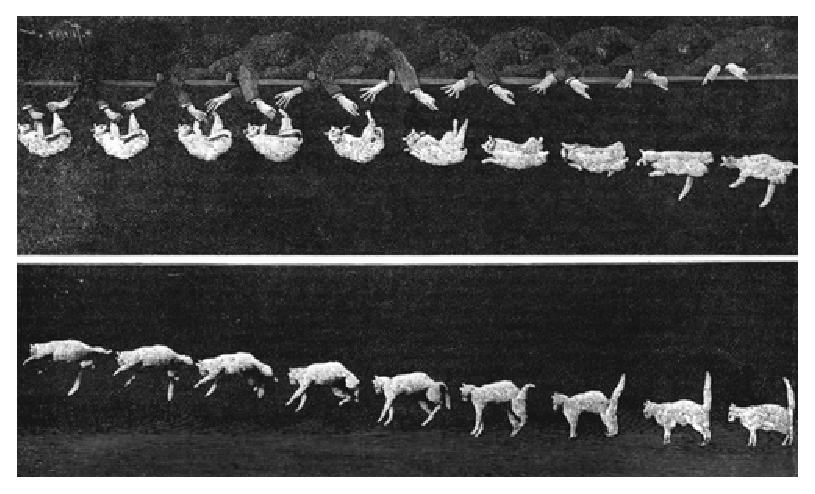
\includegraphics{Falling_cat_1894.eps}}
            \caption[Cat is changing its orientation during a fall to land on its paws.]{
                Cat changes its orientation while falling even though its
                angular momentum is initially zero and conserved during a fall.
                Snapshots of a short film recorded by \'Etienne-Jules Marey in
                1894 \cite{FallingCat}.
            }
            \label{fig.falling_cat}
        \end{figure}
\end{itemize}
%


%%%%%%%%%%%%%%%%%%%%%%%%%%%%%%%%%%%%%%%%%%%%%%%%%%%%%%%%%%%%%%%%%%%%%%%%%%%%%%%%
\subsection{Nonlinear point-mass model}\label{sec.point_mass_nonlinear}

In order to construct this model we introduce additional assumptions. Also, we
facilitate derivations by manipulating the position and orientation of the
global frame. In practice, however, it may be more convenient to utilize models
in convenient working frames and transform data to the global frame when
necessary. In many cases it is beneficial to choose the orientation of the
global (working) frame so that
%
\begin{description}
    \item[\ass{ass.gravity_z_aligned}] its $z$ axis is parallel to the gravity
        vector $\V{g}$, \IE, $\V{g}^{xy} = \V{0}$.
\end{description}
%
Also, we simplify derivations by taking the orientation of $\FRAME{c}$ to be
the same as the orientation of the global (working) frame, \IE, $\V{\LM} =
\V[c]{\LM}$ and $\dotV{\LM} = \dotV[c]{\LM}$.


The characteristic feature of the point-mass model is the absence of angular
momentum $\V[c]{\AM} = \V{0}$, since all the mass of the robot is concentrated
in a point. Note that in spite of the popularity of such point-mass
approximations, it is not strictly necessary to neglect angular momentum to
construct a linear model.

We start with \nameref{model.NMB} model, but this time we express it with
respect to the global (working) frame
%
\begin{subequations}\label{eq.simplified_system1}
\begin{empheq}[left=\empheqlbrace]{align}
    &
        \begin{bmatrix}
            \dotV{\LM} \\
            \dotV{\AM}
        \end{bmatrix}
        =
        \begin{bmatrix}
            \dotV[c]{\LM} \\
            \dotV[c]{\AM} + \V{c} \CROSS \dotV[c]{\LM}\\
        \end{bmatrix}
        =
        \begin{bmatrix}
            m \ddotV{c} \\
            \dotV[c]{\AM} + m \V{c} \CROSS \ddotV{c}\\
        \end{bmatrix}
        =
        \begin{bmatrix}
            m\V{g}\\
            m \V{c} \CROSS \V{g}
        \end{bmatrix}
        +
        \sum_{i=1}^M
            \begin{bmatrix}
                \M{I}             & \M{0}\\
                \CROSS[\contact_i]  & \M{I}
            \end{bmatrix}
            \begin{bmatrix}
                \force_i\\
                \moment_i
            \end{bmatrix}
        ,
        \label{eq.simplified_system1.dynamics}\\
    & \force_i = \M{V}_i \V{\lambda}_i,
        \\
    &
        \objA_{\moment,i}
        \begin{bmatrix}
            \V{\lambda}_i\\
            \moment_i
        \end{bmatrix}
        \ge
        \ubarV{\objb}_{\moment,i}
        ,
        \label{eq.simplified_system1.moments}
        \\
    & \V{\lambda}_i \ge \V{0},
        \label{eq.simplified_system1.friction}
        \\
    & \mbox{proxy constraints}.
        \label{eq.simplified_system1.fixedcontact}
\end{empheq}
\end{subequations}
%
Then we assume that
%
\begin{description}
    \item[\ass{ass.coplanar_contacts}] the support (ground) surface is flat, is
        spanned by $x$ and $y$ axes of the global (working) frame, and intersects $z$
        axis at $\contactC^z$,
\end{description}
%
and divide the set of all contacts into two groups:
%
\begin{enumerate}
    \item one contains all $\{1, ..., M_s\}$ support contacts, such that
        $\contactC^z_i = \contactC^z$;

    \item another contains all remaining contacts.
\end{enumerate}
%
For simplicity, all forces corresponding to the contacts of the second group
are reduced to a single wrench $(\forceext, \momentext)$ acting on the
\ac{CoM}. This wrench is used, for example, to model interaction with a
human-collaborator \cite{Agravante2016icra}, but usually it is taken to be zero.
Once this is done, the equation for the rates of momenta is transformed to
%
\begin{subequations}
    \begin{empheq}[left=\empheqlbrace]{align}
        &
        m
        \ddotV{c}
        -
        m
        \V{g}
        -
        \forceext
        =
        \sum_{i = 1}^{M_s}
        \force_i
        =
        \force_s
        \\
        &
        \dotV[c]{\AM}
        +
        \V{c}
        \CROSS
        \force_s
        -
        \momentext
        =
        \sum_{i=1}^{M_s}
        \left(
            \contact_i
            \CROSS
            \force_i
            +
            \moment_i
        \right),
    \end{empheq}
\end{subequations}
%
where $\force_s$ is the total support surface reaction force. Each contact
position can be represented by a sum of two vectors $\contact_i =
(\contact_i^{xy}, 0) + (\V{0}, \contactC^z)$, hence
%
\begin{equation}\label{eq.contact_height}
    \sum_{i=1}^{M_s}
        \contact_i
        \CROSS
        \force_i
    =
    \begin{bmatrix}
        \V{0}\\
        \contactC^z
    \end{bmatrix}
    \CROSS
    \underbrace{
    \left(
    \sum_{i=1}^{M_s}
        \force_i
    \right)}_{\force_s}
    +
    \sum_{i=1}^{M_s}
        \begin{bmatrix}
            \contact_i^{xy}\\
            0
        \end{bmatrix}
        \CROSS
        \force_i\\
\end{equation}
%

Substitution of \cref{eq.contact_height} into the equation for the rate of
angular momentum yields
%
\begin{equation}
    \dotV[c]{\AM}
    +
    \begin{bmatrix}
        0      &   \contactC^z - c^z  &   c^y\\
        c^z - \contactC^z   &   0      &   -c^x\\
        -c^y   &   c^x    &   0 \\
    \end{bmatrix}
    \force_s
    -
    \momentext
    =
    \sum_{i=1}^{M_s}
    \left(
        \begin{bmatrix}
            0               &   0               &   \contactC_i^y\\
            0               &   0               &   -\contactC_i^x\\
            -\contactC_i^y  &   \contactC_i^x   &   0 \\
        \end{bmatrix}
        \force_i
        +
        \moment_i
    \right).
\end{equation}
%
We avoid nonlinearity of this equation by assuming that
%
\begin{description}
    \item[\ass{ass.arbitrary_z_moment}] moments about the $z$ axis
        $\momentC_i^z$ can be arbitrary and the $z$ component of constraint
        \cref{eq.simplified_system1.moments} can be omitted.
\end{description}
%
Then $\dotC[c]{\AM}^z$ can be always set to any desired value, for example
zero, and the respective equation can be neglected. Provided that
%
\begin{description}
    \item[\ass{ass.nonzero_z_force}] $\forceC_s^z \ne 0$, which implies $m
        \ddotC{c}^z \ne m \C{g}^z + \forceextC^z$, \IE, the robot interacts
        with the support surface,
\end{description}
%
we divide the remaining equations for the rates of angular momentum by the
total vertical force $\forceC_s^z$
%
\begin{equation}
    \setlength{\arraycolsep}{2pt}
    \frac{
        1
    }
    {
        \forceC_s^z
    }
    \left(
        \dotC[c]{\AM}^{xy} \\
        +
        \begin{bmatrix}
            0      &   \contactC^z -c^z   &   c^y\\
            c^z - \contactC^z   &   0      &   -c^x\\
        \end{bmatrix}
        \force_s
        -
        \momentext^{xy}
    \right)
    =
    \frac{
        1
    }
    {
        \forceC_s^z
    }
        \sum_{i=1}^{M_s}
        \left(
            \forceC_i^z
            \begin{bmatrix}
                \contactC_i^y  \\
                -\contactC_i^x \\
            \end{bmatrix}
            +
            \moment_i^{xy} \\
        \right)
    =
    \frac{
        \moment_{s}^{xy} \\
    }
    {
        \forceC_s^z
    }
\end{equation}
%
where $\moment_{s}^{xy}$ is the total moment created by the surface contacts.
Then the rightmost expression is equal to $(\copC^y, -\copC^x)$ as shown in
\cref{sec.rectangular_foot}, and $(\copC^x, \copC^y)$ is the position of the
\ac{CoP} of all support contacts. In this context the \ac{CoP} is also known as
\ac{ZMP}, since the moments about the $x$ and $y$ axes are zero in this point
\cite{Vukobratovic2004ijhr}. The \ac{CoP} must stay within the \tn{support
area} -- the convex hull of all support contacts illustrated in
\cref{fig.support_area}: $\cop \in \SET{S}(\contact_1^{xy}, ...
,\contact_{M_s}^{xy})$. This constraint on the position of the \ac{CoP} is
equivalent to the remaining constraints on $x$ and $y$ components of contact
moments in \cref{eq.simplified_system1.moments} as follows from
\cref{sec.rectangular_foot,sec.surface_contacts}.


\begin{figure}[ht]
    \centering{%
    \includegraphics{support_area.eps}}
    \caption[Support area of two rectangular feet.]{
        Grey area represents support area $\SET{S}(\contact_1^{xy},
        \contact_2^{xy})$ of two rectangular foot contacts.
    }
    \label{fig.support_area}
\end{figure}


Now we drop individual support contact forces and moments $(\force_i,
\moment_i)$ with $i \in \{1, ..., M_s\}$ to obtain
%
\begin{subequations}\label{eq.no_ground_contact_forces}
    \begin{empheq}[left=\empheqlbrace]{align}
        &
            \force_s
            =
            m
            (\ddotV{c} - \V{g})
            -
            \forceext
            =
            \sum_{i = 1}^{M_s}
                \M{V}_i \V{\lambda}_i
            ,
            \\
        &
            \frac{1}{\forceC_s^z}
            \left(
                \dotV[c]{\AM}^{xy}
                -
                \momentext^{xy}
                -
                (
                    c^z
                    -
                    \contactC^z
                )
                \begin{bmatrix}
                    \forceC_s^y \\
                    -\forceC_s^x\\
                \end{bmatrix}
            \right)
            +
            \begin{bmatrix}
                c^y\\
                -c^x\\
            \end{bmatrix}
            =
            \begin{bmatrix}
                \copC^y\\
                -\copC^x
            \end{bmatrix},
            \\[2mm]
        &
            \cop \in \SET{S}(\contact_1^{xy}, ... ,\contact_{M_s}^{xy})
            ,
            \\
        & \V{\lambda}_i \ge \V{0},
            \\
        & \forceC_s^z \ne 0,
            \label{eq.no_ground_contact_forces.nonzero_z_force}
            \\
        & \mbox{proxy constraints}.
    \end{empheq}
\end{subequations}
%
The system is further simplified if
%
\begin{description}
    \item[\ass{ass.point_mass}] The rate of angular momentum is always zero
        $\V[c]{\AM}^{xy} = \V{0}$, which implies that the system models a
        point-mass. This is an ubiquitous assumption in the literature, even
        though it is not required to construct a linear model
        \cite{Wieber2015handbook}.

    \item[\ass{ass.same_friction}] The friction coefficients are the same for
        all contacts, so that $\M{V}_i = \M{V}$ and
        %
        $
            \force_s = \V{V} \sum_{i = 1}^{M_s} \V{\lambda}_i
            \quad
            \mbox{or}
            \quad
            \force_s = \M{V} \V{\lambda}
        $
        %
        with $\V{\lambda} \ge \V{0}$, which makes variables $\V{\lambda}_i$
        unnecessary.
\end{description}
%
\cref{ass.same_friction} implies that the total surface contact force is
constrained to the same friction cone as individual surface contact forces.


Thus, the system takes the following form
%
\begin{model}{NPM}{Nonlinear Point-Mass}
\begin{subequations}\label{eq.nonlinear_point_mass}
    \begin{empheq}[left=\empheqlbrace]{align}
        &
            \cop
            =
            \V{c}^{xy}
            -
            \zeta
            \force_s^{xy} / m
            +
            \frac{1}{\forceC_s^z}
            \begin{bmatrix}
                - \momentextC^y \\
                \momentextC^x \\
            \end{bmatrix}
            ,
            \\
        &
            \zeta
            =
            \frac{m (c^z - \contactC^z)}{\forceC_s^z}
            ,
            \\[2mm]
        &
            \cop \in \SET{S}(\contact_1^{xy}, ... ,\contact_{M_s}^{xy})
            ,
            \label{eq.nonlinear_point_mass.cop_ctr}
            \\
        & \forceC_s^z \ne 0,
            \label{eq.nonlinear_point_mass.nonzero_z_force}
            \\
        &
            \force_s
            =
            m
            (\ddotV{c} - \V{g})
            -
            \forceext
            =
            \M{V} \V{\lambda}
            ,
            \quad
            \V{\lambda} \ge \V{0}
            ,
            \label{eq.nonlinear_point_mass.friction}
            \\
        & \mbox{proxy constraints}
            ,
            \label{eq.nonlinear_point_mass.proxy}
    \end{empheq}
\end{subequations}
\end{model}
%
where the first equation is nonlinear with respect to motion of the \ac{CoM}
and external force $\forceext$, and constraint
\cref{eq.nonlinear_point_mass.cop_ctr} is nonlinear with respect to positions
and orientations of the contacts as explained in \cref{sec.surface_contacts}.



%%%%%%%%%%%%%%%%%%%%%%%%%%%%%%%%%%%%%%%%%%%%%%%%%%%%%%%%%%%%%%%%%%%%%%%%%%%%%%%%
%%%%%%%%%%%%%%%%%%%%%%%%%%%%%%%%%%%%%%%%%%%%%%%%%%%%%%%%%%%%%%%%%%%%%%%%%%%%%%%%
%%%%%%%%%%%%%%%%%%%%%%%%%%%%%%%%%%%%%%%%%%%%%%%%%%%%%%%%%%%%%%%%%%%%%%%%%%%%%%%%
\section{Linear approximate models}\label{sec.linear_approx_models}

In the present work we employ two types of approximate models: the first one
(\cref{sec.model_momenta}) is tailored for 3-dimensional multi-contact
settings, the second (\cref{sec.point_mass_planar,sec.point_mass_nonplanar}) --
for walking. All of these models are based on the models described in
\cref{sec.nonlinear_approx_models} and are linear. Though nonlinear models find
more and more applications in practice, they are generally more demanding for
computational resources \cite{Koenemann2015iros}.



%%%%%%%%%%%%%%%%%%%%%%%%%%%%%%%%%%%%%%%%%%%%%%%%%%%%%%%%%%%%%%%%%%%%%%%%%%%%%%%%
\subsection{Momenta-based model with noncoplanar contacts}\label{sec.model_momenta}

The linear model for preview of linear and angular momenta derived in this
section was originally proposed in \cite{Nagasaka2012} in Japanese and later
restated with some minor extensions in \cite{Audren2014iros,
Sherikov2015humanoids} in English.


The component-wise equation of rate of angular momentum in \nameref{model.NMB}
model has the following form
%
\begin{equation}\label{eq.component_wise_momenta}
    \begin{bmatrix}
        \dotC[c]{\AM}^x\\
        \dotC[c]{\AM}^y\\
        \dotC[c]{\AM}^z
    \end{bmatrix}
    =
    \sum_{i=1}^M
    \left(
        \begin{bmatrix}
            0                   & - (\contactC_i^z - {c}^z)   & \contactC_i^y - {c}^y \\
            \contactC_i^z - {c}^z     & 0                     & - (\contactC_i^x - {c}^x)\\
            - (\contactC_i^y - {c}^y) & \contactC_i^x - {c}^x       & 0
        \end{bmatrix}
        \begin{bmatrix}
            \forceC_i^x\\
            \forceC_i^y\\
            \forceC_i^z
        \end{bmatrix}
        +
        \begin{bmatrix}
            \momentC_i^x\\
            \momentC_i^y\\
            \momentC_i^z
        \end{bmatrix}
    \right).
\end{equation}
%
In order to avoid nonlinearity in this equation we assume that
%
\begin{description}
    \item[\ass{ass.fixed_points}] Contact points $\contact_i$ are given constants.

    \item[\ass{ass.fixed_z_coordinate}] $\C{c}^z$ is a given constant, which
        implies that the \ac{CoM} acceleration along the $z$ axis is zero and
        %
        \begin{equation}
            \dotC{\LM}^z
            =
            m
            \ddot{c}^z
            =
            m
            g^z
            +
            \sum_{i=1}^M
                \forceC_i^z
            =
            0.
        \end{equation}
        %

    \item[\ass{ass.arbitrary_z_momentum}] Rate of angular momentum about the
        $z$ axis is arbitrary. In other words, the computed rotational motion
        about the $z$ axis is always feasible. Validity of this assumption is
        not completely clear, but no problems in simulations were reported so
        far. This assumption is opposite to \cref{ass.arbitrary_z_moment},
        which allows for arbitrary contact moments about the $z$ axis in the
        point-mass (\nameref{model.NPM}) model.
\end{description}
%


Since the vertical motion of the \ac{CoM} is prohibited by
\cref{ass.fixed_z_coordinate} and $\dotC[c]{\AM}^z$ is neglected due to
\cref{ass.arbitrary_z_momentum}, we focus on the linear and angular momenta
about the $x$ and $y$ axes:
%
\begin{align}\label{eq.dynamics_momenta_model}
    \dotV{\LM}^{xy}
    &
    =
    m
    \ddotV{c}^{xy}
    =
    \underbrace{
        m
        \V{g}^{xy}
    }_{\tildeV{b}}
    +
    \sum_{i=1}^M
        \force_i^{xy}
    \\
    \dotV[c]{\AM}^{xy}
    &
    =
    \sum_{i=1}^M
    \Bigg(
        \underbrace{
            \begin{bmatrix}
                0                   & - (\contactC_i^z - {c}^z)   & \contactC_i^y\\
                \contactC_i^z - {c}^z     & 0                     & - \contactC_i^x\\
            \end{bmatrix}
        }_{\tildeM{B}_{i}}
        \force_i
        +
        \Ixy
        \moment_i
    \Bigg)
    +
    \underbrace{
        \begin{bmatrix}
            0     &     g^z \\
            - g^z &     0
        \end{bmatrix}
    }_{\tildeM{A}}
    \underbrace{
        (
            m \V{c}^{xy}
        )
    }_{\hatV{\LM}^{xy}}
\end{align}
%
Then we construct a linear continuous-time model with $M$ control inputs
$\wrench_i = (\force_i, \moment_i)$ and state vector $\V{x} = (m \V{c}^{xy},
\V{\LM}^{xy}, \V[c]{\AM}^{xy}) = (\hatV{\LM}^{xy}, \V{\LM}^{xy},
\V[c]{\AM}^{xy})$:
%
\begin{model}{CMB}{Continuous Momenta-Based}
\begin{subequations}\label{eq.continuous_momenta_model}
\begin{empheq}[left=\empheqlbrace]{align}
    &
        \underbrace{
            \begin{bmatrix}
                \V{\LM}^{xy}\\
                \dotV{\LM}^{xy}\\
                \dotV[c]{\AM}^{xy}
            \end{bmatrix}
        }_{\dotV{x}}
        =
        \underbrace{
            \begin{bmatrix}
                \V{0}         & \V{I}   & \V{0}\\
                \V{0}         & \V{0}   & \V{0}\\
                \tildeM{A}  & \V{0}   & \V{0}
            \end{bmatrix}
        }_{\M{A}}
        \underbrace{
            \begin{bmatrix}
                \hatV{\LM}^{xy}\\
                \V{\LM}^{xy}\\
                \V[c]{\AM}^{xy}
            \end{bmatrix}
        }_{\V{x}}
        +
        \sum_{i=1}^M
        \underbrace{
            \begin{bmatrix}
                \V{0}             & \V{0}\\
                \Ixy                    & \V{0}\\
                \tildeM{B}_{i}          & \Ixy
            \end{bmatrix}
        }_{\M{B}_i}
        \underbrace{
            \begin{bmatrix}
                \force_i \\
                \moment_i
            \end{bmatrix}
        }_{\wrench_i}
        +
        \underbrace{
            \begin{bmatrix}
                \V{0}\\
                \tildeV{b}\\
                \V{0}
            \end{bmatrix}
        }_{\V{b}}
        \label{eq.continuous_momenta_model.dynamics}
        \\
    & \force_i = \M{V}_i \V{\lambda}_i
        ,
      \\
    &
        \sum_{i=1}^M \forceC_i^z = - m g^z
        ,
        \\
    &
        \objA_{\moment,i}
        \begin{bmatrix}
            \V{\lambda}_i\\
            \moment_i
        \end{bmatrix}
        \ge
        \ubarV{\objb}_{\moment,i}
        ,
        \\
    & \V{\lambda}_i \ge \V{0},
        \label{eq.continuous_momenta_model.friction}\\
    & \mbox{proxy constraints}.
        \label{eq.continuous_momenta_model.fixedcontact}
\end{empheq}
\end{subequations}
\end{model}
%
Note that if \cref{ass.gravity_z_aligned} holds, \IE, $\V{g}^{xy} = \V{0}$, the
model is simplified due to $\V{b} = \V{0}$. \cref{ass.gravity_z_aligned} may be
too restrictive in some applications \cite{Audren2014iros}, but in the
simulations discussed in \cref{sec.optional_force} it always holds true.



%%%%%%%%%%%%%%%%%%%%%%%%%%%%%%%%%%%%%%%%%%%%%%%%%%%%%%%%%%%%%%%%%%%%%%%%%%%%%%%%
\subsection{Linear point-mass model with planar CoM motion}\label{sec.point_mass_planar}

The subject of the present section is the \tn{linear point-mass model}, which
was originally proposed by Kajita \cite{Kajita2001icra, Kajita2003icra}, later
it was employed and extended in \cite{Diedam2008iros, Herdt2010auro,
Agravante2016icra} and many other works. The best known variant of this model
is interpreted as an \tn{inverted pendulum} with a weightless leg and a mass
constrained to a plane as shown in \cref{fig.inverted_pendulum}. Hence, it is
often referred to as \ac{LIPM} in the literature.

\begin{figure}[ht]
    \centering{%
    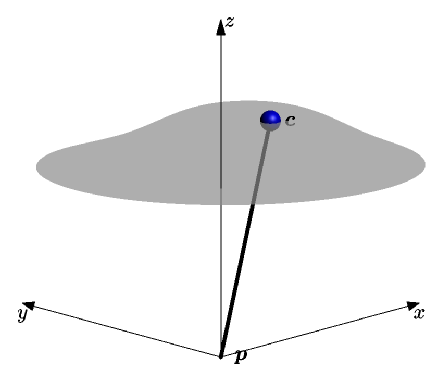
\includegraphics{inverted_pendulum.eps}}
    \caption{Inverted pendulum with a mass $\V{c}$ constrained to a plane.}
    \label{fig.inverted_pendulum}
\end{figure}


\nameref{model.NPM} model is usually linearized with respect to the \ac{CoM}
motion by taking $\C{c}^z$ to be constant and, consequently, $\ddotC{c}^z = 0$
(\cref{ass.fixed_z_coordinate}) \cite{Kajita2003icra}. In addition to this the
following assumptions are commonly made
%
\begin{description}
    \item[\ass{ass.known_ext_wrench}] Wrench $(\forceext,\momentext)$ is known,
        or $\forceextC^z = 0$. This is necessary to linearize the model with
        respect to the external wrench \cite{Agravante2016icra}. In the
        following we assume that $(\forceext,\momentext)$ is a known constant
        for simplicity.

    \item[\ass{ass.linear_convex_hull}] Constraint
        \cref{eq.nonlinear_point_mass.cop_ctr} on the \ac{CoP} positions is
        expressed with a set of linear equality and inequality constraints. The
        conditions under which this is true are discussed in
        \cref{sec.surface_contacts}.

    \item[\ass{ass.sufficient_friction}] Proxy constraints
        \cref{eq.nonlinear_point_mass.proxy} and constraints on the surface
        contact forces
        \cref{eq.nonlinear_point_mass.friction,eq.nonlinear_point_mass.nonzero_z_force}
        are always satisfied. They can, however, be imposed explicitly if
        necessary.
\end{description}
%
Then the model is reduced to
%
\begin{subequations}\label{eq.linear_point_mass}
    \begin{empheq}[left=\empheqlbrace]{align}
        &
            \cop
            =
            \V{c}^{xy}
            -
            \zeta
            \ddotV{c}^{xy}
            +
            \FUNC{Z}(\zeta, \V{g}, \forceext, \momentext)
            ,
            \label{eq.linear_point_mass.cop_eq}
            \\
        &
            \zeta
            =
            \frac{m (c^z - \contactC^z)}{- m \C{g}^z - \forceextC^z}
            ,
            \\[2mm]
        &
            \cop \in \SET{S}(\contact_1^{xy}, ... ,\contact_{M_s}^{xy})
            ,
            \label{eq.linear_point_mass.cop_ctr}
    \end{empheq}
\end{subequations}
%
where the function $\FUNC{Z}(\zeta, \V{g}, \forceext, \momentext)$ represents
the contribution of the external wrench and gravity to the \ac{CoP} position:
%
\begin{equation}
    \FUNC{Z}(\zeta, \V{g}, \forceext, \momentext)
    =
    \zeta
    \left(
        \V{g}^{xy}
        +
        \frac{\forceext^{xy}}{m}
    \right)
    +
    \frac{1}{- m \C{g}^z - \forceextC^z}
    \begin{bmatrix}
        - \momentextC^y\\
        \momentextC^x\\
    \end{bmatrix}
    ,
\end{equation}
%
The model can be further combined with a double or triple integrator to obtain
a second or third order linear model. There is a number of ways to realize such
a combination. For example, the \ac{CoP} position can be
%
\begin{itemize}
    \item an output of second or third order model \cite{Kajita2003icra,
        Herdt2010auro, Agravante2016icra};

    \item a part of the state of a third order model \cite{Kajita2010iros};

    \item the control input of a second order or third order model
        \cite{Sherikov2014humanoids}.
\end{itemize}
%
Furthermore, the differential equation \cref{eq.linear_point_mass.cop_eq} can
be transformed to expose its stable and unstable parts
\cite{Englsberger2011iros, Krause2012src, Takenaka2009iros}, see also
\cref{sec.point_mass_planar_capturability}. Another common approach taken in
the literature consist in collapsing the surface contacts to point contacts,
which greatly simplifies constraint \cref{eq.linear_point_mass.cop_ctr}
\cite{Englsberger2011iros}: if $M_s = 1$ then $\cop = \contact_1^{xy}$, if $M_s
= 2$ then $\cop$ lies on a segment $[\contact_1^{xy}, \contact_2^{xy}]$, \ETC.
The differences between the various versions of the model are often subtle, but
there are certain general considerations to keep in mind while choosing a
particular version:
%
\begin{itemize}
    \item Force sensors in the feet of modern robots allow for the
        determination of the position of the \ac{CoP}
        \cite{Englsberger2014humanoids, Kaneko2004icra, Kaneko2009humanoids},
        which suggests its inclusion into the state of the model.

    \item Third order models imply a smooth variation of \ac{CoM} acceleration
        contrary to second order models. A discontinuous change of \ac{CoM}
        acceleration results in a discontinuous change of the \ac{CoP}
        position, which are difficult to realize for humanoid robots
        \cite{Kajita2010iros}.

    \item Discretization of models controlled with piece-wise constant \ac{CoM}
        acceleration or \tn{jerk} (derivative of acceleration) leads to some
        minor difficulties in the satisfaction of constraint
        \cref{eq.linear_point_mass.cop_ctr}. Moreover, the number of times this
        constraint is imposed can be larger than in other cases and its
        satisfaction is not guaranteed at all times. These issues are discussed
        later in \cref{sec.point_mass_planar_discret_jerk}, where the models
        are discretized to be used in \ac{MPC} schemes.
\end{itemize}
%


In the following we are going to consider two third order models, whose state
includes positions, velocities, and accelerations of the \ac{CoM} in the
$x$-$y$ plane
%
\begin{equation}
    \V{x} =
    (
        \C{c}^x,
        \dotC{c}^x,
        \ddotC{c}^x,
        \C{c}^y,
        \dotC{c}^y,
        \ddotC{c}^y
    ).
\end{equation}
%
The models differ in their control inputs:
%
\begin{enumerate}
    \item The first one is controlled by the third derivative (\tn{jerk}) of
        the \ac{CoM} position~\cite{Kajita2003icra, Herdt2010auro,
        Agravante2016icra}
        %
        \begin{model}{CPPMJ}{Continuous Planar Point-Mass controlled with \acs{CoM} Jerk}
        \begin{subequations}\label{eq.point_mass_jerk_control}
            \begin{empheq}[left=\empheqlbrace]{align}
                &
                    \dotV{x}
                    =
                    \begin{bmatrix}
                        \tildeM{A}  & \M{0} \\
                        \M{0} & \tildeM{A}  \\
                    \end{bmatrix}
                    \V{x}
                    +
                    \begin{bmatrix}
                        \tildeV{B} & \V{0}\\
                        \V{0} & \tildeV{B} \\
                    \end{bmatrix}
                    \dddotV{c}^{xy}
                    ,
                    \\
                &
                    \cop
                    =
                    \begin{bmatrix}
                        \tildeM{D} & \M{0}\\
                        \M{0} & \tildeM{D}\\
                    \end{bmatrix}
                    \V{x}
                    +
                    \FUNC{Z}(\zeta, \V{g}, \forceext, \momentext)
                    ,
                    \label{eq.point_mass_jerk_control.cop}
                    \\[2mm]
                &
                    \cop \in \SET{S}(\contact_1^{xy}, ... ,\contact_{M_s}^{xy})
                    ,
            \end{empheq}
        \end{subequations}
        \end{model}
        %
        where
        %
        \begin{equation}
            \tildeM{A}
            =
            \begin{bmatrix}
                0   &  1    & 0    \\
                0   &  0    & 1    \\
                0   &  0    & 0 \\
            \end{bmatrix},
            \quad
            \tildeV{B}
            =
            \begin{bmatrix}
                0  \\
                0  \\
                1  \\
            \end{bmatrix},
            \quad
            \tildeM{D}
            =
            \begin{bmatrix}
                1 & 0 &  - \zeta
            \end{bmatrix}
            .
        \end{equation}
        %
        We do not use this model in our controllers and present it here due to
        its prevalence in the literature.


    \item The second one is controlled by the \ac{CoP} velocity, which is
        obtained by differentiation of \cref{eq.linear_point_mass.cop_eq} under
        assumption that $(\forceext, \momentext)$ is constant
        \cite{Sherikov2014humanoids}
        %
        \begin{model}{CPPMdZ}{Continuous Planar Point-Mass controlled with $\dot{\cop}$}
        \begin{subequations}\label{eq.point_mass_cop_control}
            \begin{empheq}[left=\empheqlbrace]{align}
                &
                    \dotV{x}
                    =
                    \begin{bmatrix}
                        \tildeM{A}  & \M{0} \\
                        \M{0} & \tildeM{A}  \\
                    \end{bmatrix}
                    \V{x}
                    +
                    \begin{bmatrix}
                        \tildeV{B} & \V{0}\\
                        \V{0} & \tildeV{B} \\
                    \end{bmatrix}
                    \dot{\cop},
                    \\
                &
                    \cop
                    =
                    \begin{bmatrix}
                        \tildeM{D} & \M{0}\\
                        \M{0} & \tildeM{D}\\
                    \end{bmatrix}
                    \V{x}
                    +
                    \FUNC{Z}(\zeta, \V{g}, \forceext, \momentext)
                    ,
                    \\[2mm]
                &
                    \cop \in \SET{S}(\contact_1^{xy}, ... ,\contact_{M_s}^{xy})
                    ,
            \end{empheq}
        \end{subequations}
        \end{model}
        %
        where
        %
        \begin{equation}
            \tildeM{A}
            =
            \begin{bmatrix}
                0   &  1  &   0 \\
                0   &  0  &  1 \\
                0   &  \frac{1}{\zeta}   &  0   \\
            \end{bmatrix},
            \quad
            \tildeV{B}
            =
            \begin{bmatrix}
                0   \\
                0   \\
                -\frac{1}{\zeta}\\
            \end{bmatrix}
            , \quad
            \tildeM{D}
            =
            \begin{bmatrix}
                1 & 0 &  - \zeta
            \end{bmatrix}
            .
        \end{equation}
        %
        Here we assumed that
        %
        \begin{description}
            \item[\ass{ass.nonzero_com_height}] $\zeta \ne 0$ or $c^z -
                \contactC^z \ne 0$, \IE, the \ac{CoM} position is not in
                the same plane as contacts.
        \end{description}
        %
        If \cref{ass.nonzero_com_height} does not hold, \nameref{model.CPPMJ}
        and \nameref{model.CPPMdZ} models become equivalent.
\end{enumerate}
%



%%%%%%%%%%%%%%%%%%%%%%%%%%%%%%%%%%%%%%%%%%%%%%%%%%%%%%%%%%%%%%%%%%%%%%%%%%%%%%%%
\subsection{Linear point-mass model with nonplanar CoM motion}\label{sec.point_mass_nonplanar}

Walking with planar motion of the \ac{CoM} (\cref{ass.fixed_z_coordinate}) is
considered to be unnatural and inefficient in terms of energy. In order to
address these issues we proposed to construct a model, which allows for
vertical motion of the \ac{CoM} \cite{Brasseur2015humanoids}. This is achieved
by making the model robust to the motion of the \ac{CoM} along the $z$ axis.


Let us consider \nameref{model.NPM} model
%
\begin{subequations}
    \begin{empheq}[left=\empheqlbrace]{align}
        &
            \cop
            =
            \V{c}^{xy}
            -
            \zeta
            \left(
                \ddotV{c}^{xy} - \V{g}^{xy}  - \frac{\forceext^{xy}}{m}
            \right)
            +
            \underbrace{
                \frac{1}{m (\ddotC{c}^z - \C{g}^z) - \forceextC^z}
            }_{\zeta / (m c^z)}
            \begin{bmatrix}
                - \momentextC^y \\
                \momentextC^x \\
            \end{bmatrix}
            ,
            \\
        &
            \zeta
            =
            \frac{m c^z}{m (\ddotC{c}^z - \C{g}^z) - \forceextC^z}
            ,
            \\[2mm]
        &
            \cop \in \SET{S}(\contact_1^{xy}, ... ,\contact_{M_s}^{xy})
            ,
    \end{empheq}
\end{subequations}
%
where some of the constraints are omitted for simplicity and the support area
is assumed to be linear with respect to contact points
(\cref{ass.sufficient_friction,ass.linear_convex_hull}). One can observe that
if
%
\begin{description}
    \item[\ass{ass.ext_wrench_zero}] the external wrench is equal to zero
        $(\forceext, \momentext) = \V{0}$,
\end{description}
%
the position of the \ac{CoP} is linear with respect to parameter $\zeta$:
%
\begin{subequations}
    \begin{empheq}[left=\empheqlbrace]{align}
        &
            \cop^{xy}
            =
            \V{c}^{xy}
            -
            \zeta
            (
                \ddotV{c}^{xy} - \V{g}^{xy}
            )
            ,
            \\
        &
            \zeta
            =
            \frac{c^z - \contactC^z}{\ddotC{c}^z - \C{g}^z}
            ,
            \\[2mm]
        &
            \cop \in \SET{S}(\contact_1^{xy}, ... ,\contact_{M_s}^{xy})
            .
    \end{empheq}
\end{subequations}
%
Thus, if $\zeta$ is bounded $\ubar{\zeta} \le \zeta \le \bar{\zeta}$, the
\ac{CoP} position $\cop$ lies on a line segment between two points
$\ubar{\cop}$ and $\bar{\cop}$ as shown in \cref{fig.support_area_zeta}, where
%
\begin{equation}
    \ubar{\cop}
    =
    \V{c}^{xy}
    -
    \ubar{\zeta}
    (\ddotV{c}^{xy} - \V{g}^{xy}),
    \quad
    \bar{\cop}
    =
    \V{c}^{xy}
    -
    \bar{\zeta}
    (\ddotV{c}^{xy} - \V{g}^{xy}).
\end{equation}
%
\begin{figure}[ht]
    \centering{%
    \includegraphics{support_area_zeta.eps}}
    \caption[Robust constraints on the Center of Pressure position.]{
        Grey area represents support area $\SET{S}(\contact_1^{xy},
        \contact_2^{xy})$ of two rectangular foot contacts. The \ac{CoP}
        position lying on a line segment between two points is shown in red.
    }%
    \label{fig.support_area_zeta}%
\end{figure}%
%
At the same time, $\ubar{\cop} \in \SET{S}(\contact_1^{xy}, ... ,
\contact_{M_s}^{xy})$ and $\bar{\cop} \in \SET{S}(\contact_1^{xy}, ... ,
\contact_{M_s}^{xy})$ imply $\cop \in \SET{S}(\contact_1^{xy}, ... ,
\contact_{M_s}^{xy})$ due to convexity of the support area (see
\cref{fig.support_area_zeta}). Hence, we construct a system of linear
constraints on the 3-dimensional motion of the \ac{CoM} as follows
%
\begin{subequations}
    \begin{empheq}[left=\empheqlbrace]{align}
        &
            \ubar{\cop}
            =
            \V{c}^{xy}
            -
            \ubar{\zeta}
            (\ddotV{c}^{xy} - \V{g}^{xy})
            ,
            \\
        &
            \bar{\cop}
            =
            \V{c}^{xy}
            -
            \bar{\zeta}
            (\ddotV{c}^{xy} - \V{g}^{xy}),
            \\
        &
            \ubar{\zeta} (\ddotC{c}^z - \C{g}^z)
            \le
            c^z - \contactC^z
            \le
            \bar{\zeta} (\ddotC{c}^z - \C{g}^z)
            ,
            \\
        &
            \ubar{\cop} \in \SET{S}(\contact_1^{xy}, ... ,\contact_{M_s}^{xy})
            ,
            \\
        &
            \bar{\cop} \in \SET{S}(\contact_1^{xy}, ... ,\contact_{M_s}^{xy})
            ,
    \end{empheq}
\end{subequations}
%
where $\ubar{\zeta}$ and $\bar{\zeta}$ are predefined constants. This system
is then combined with the triple integrator to model motion of the \ac{CoM}
%
\begin{model}{CNPM}{Continuous Nonplanar Point-Mass}
\begin{subequations}
    \begin{empheq}[left=\empheqlbrace]{align}
        &
            \dotV{x}
            =
            \diag{3}{\tildeM{A}}
            \V{x}
            +
            \diag{3}{\tildeM{B}}
            \dddotV{c}
            ,
            \\
        &
            \ubar{\zeta} (\ddotC{c}^z - \C{g}^z)
            \le
            c^z - \contactC^z
            \le
            \bar{\zeta} (\ddotC{c}^z - \C{g}^z)
            ,
            \\[2mm]
        &
            \V{c}^{xy}
            -
            \ubar{\zeta}
            (\ddotV{c}^{xy} - \V{g}^{xy})
            \in
            \SET{S}(\contact_1^{xy}, ... ,\contact_{M_s}^{xy})
            ,\\
        &
            \V{c}^{xy}
            -
            \bar{\zeta}
            (\ddotV{c}^{xy} - \V{g}^{xy})
            \in
            \SET{S}(\contact_1^{xy}, ... ,\contact_{M_s}^{xy})
            ,
            \\[2mm]
        &
            \V{x} =
            (
                \C{c}^x,
                \dotC{c}^x,
                \ddotC{c}^x,
                \enspace
                \C{c}^y,
                \dotC{c}^y,
                \ddotC{c}^y,
                \enspace
                \C{c}^z,
                \dotC{c}^z,
                \ddotC{c}^z
            )
            ,
    \end{empheq}
\end{subequations}
\end{model}
%
where
%
\begin{equation}
    \tildeM{A}
    =
    \begin{bmatrix}
        0   &  1    & 0    \\
        0   &  0    & 1    \\
        0   &  0    & 0 \\
    \end{bmatrix},
    \quad
    \tildeV{B}
    =
    \begin{bmatrix}
        0  \\
        0  \\
        1  \\
    \end{bmatrix}
    .
\end{equation}
%



%%%%%%%%%%%%%%%%%%%%%%%%%%%%%%%%%%%%%%%%%%%%%%%%%%%%%%%%%%%%%%%%%%%%%%%%%%%%%%%%
%%%%%%%%%%%%%%%%%%%%%%%%%%%%%%%%%%%%%%%%%%%%%%%%%%%%%%%%%%%%%%%%%%%%%%%%%%%%%%%%
%%%%%%%%%%%%%%%%%%%%%%%%%%%%%%%%%%%%%%%%%%%%%%%%%%%%%%%%%%%%%%%%%%%%%%%%%%%%%%%%
\section{Limitations of the approximate models}\label{sec.approx_models_limitations}

We conclude our survey of approximate models with a reflection upon their
limitations and the means of relaxing these limitations. In order to do this,
we investigate the assumptions made during the derivation of these models:
%
\begin{itemize}
    \item We abstract from the complex structure of the robot's body
        (\cref{ass.nojointctr}). Hence, we lose the ability to express some of
        the whole body tasks and constraints. For example, the point-mass model
        does not allow to specify a reaching task for a hand. Therefore, when
        it is necessary to bias motion previewed with this model by a hand
        task, it is common to resort to various \emph{ad hoc} approaches
        \cite{Yoshida2006humanoids, Nishiwaki2003icra, Fukumoto2004iros}. Whole
        body constraints are often approximated by proxy constraints
        (\cref{sec.nonlinear_approx_models}). For example, the position of the
        \ac{CoM} is limited with respect to foot positions in
        \cite{Brasseur2015humanoids, Dellin2012icra} to avoid kinematic
        infeasibility. Another general approach to take into account whole body
        tasks and constraints is to employ \ac*{MMPC}, which was proposed in
        \cite{Sherikov2014humanoids} and is described in \cref{sec.mmpc}.


    \item We presume that the rate of angular momentum is zero in the
        point-mass model (\cref{ass.point_mass}) or takes arbitrary values in
        the momenta based model (\cref{sec.model_momenta}). Neither of this is
        true in reality: execution of limb motions implies certain values of
        rate of angular momentum. These values can be estimated using
        multi-mass models, some of which are linear
        \cite[Chapter~3]{Herdt2012thesis}, \cite{Lafaye2014humanoids,
        Shimmyo2013tie, Takenaka2009iros}.


    \item Bilinearity of the rate of angular momentum with respect to the
        \ac{CoM} motion and contact forces as follows from Equation
        \cref{eq.newton-euler} is addressed with two assumptions:
        %
        \begin{itemize}
            \item The angular momentum about the $z$ axis is typically
                disregarded
                (\cref{ass.arbitrary_z_momentum,ass.arbitrary_z_moment}).
                Significance of implications of this is currently unclear to
                us.

            \item Motion of the \ac{CoM} is fixed to a plane
                (\cref{ass.fixed_z_coordinate}). There exists a number of
                approaches to cope with this \cite{Nishiwaki2011icra,
                Feng2013humanoids}, in particular, we proposed to introduce
                robustness with respect to nonplanar \ac{CoM} motion
                \cite{Brasseur2015humanoids}, \cref{sec.point_mass_nonplanar}.
        \end{itemize}

        %
        \begin{equation}\label{eq.newton-euler}
            \begin{bmatrix}
                \dotV[c]{\LM} \\
                \dotV[c]{\AM}\\
            \end{bmatrix}
            =
            \begin{bmatrix}
                m\V{g}\\
                \V{0}
            \end{bmatrix}
            +
            \sum_{i=1}^M
                \begin{bmatrix}
                    \M{I}                     & \M{0}\\
                    \CROSS[(\contact_i - \V{c})]   & \M{I}
                \end{bmatrix}
                \begin{bmatrix}
                    \force_i\\
                    \M[i]{R} \moment[i]_i
                \end{bmatrix}.
        \end{equation}
        %

    \item Bilinearity of the rate of angular momentum with respect to the
        contact positions and contact forces as follows from Equation
        \cref{eq.newton-euler} is dealt with by predetermining either contact
        positions or magnitudes of the contact forces. For example, we fix
        contact positions in the momenta based model (\cref{ass.fixed_points}).
        On the other hand, in the case of a single contact, when the force is
        determined by the \ac{CoM} motion, the contact position may vary (see
        \cite{Herdt2010auro} and \cref{sec.surface_contacts}). When it is
        undesirable to predetermine contact positions and forces, it is common
        to employ nonlinear models \cite{Dai2014humanoids, Tassa2014icra}.
\end{itemize}
%

It is important to note that some of these limitations can be lifted in
discrete-time models, since such models allow for different parameters on
different discretization intervals. For example, in discrete-time the number
and positions of contacts in the momenta-based model may vary, as well as the
height of the contact surface $\contactC^z$ in the point-mass model with
nonplanar \ac{CoM} motion. This topic is discussed in more detail in
\cref{sec.discret_variation}.



%%%%%%%%%%%%%%%%%%%%%%%%%%%%%%%%%%%%%%%%%%%%%%%%%%%%%%%%%%%%%%%%%%%%%%%%%%%%%%%%
%%%%%%%%%%%%%%%%%%%%%%%%%%%%%%%%%%%%%%%%%%%%%%%%%%%%%%%%%%%%%%%%%%%%%%%%%%%%%%%%
%%%%%%%%%%%%%%%%%%%%%%%%%%%%%%%%%%%%%%%%%%%%%%%%%%%%%%%%%%%%%%%%%%%%%%%%%%%%%%%%
\section{Conclusion}

This chapter serves as a survey of the whole body model of a humanoid robot and
approximate models derived from it. The models are presented in a unified view,
which is not very common in the literature, where the focus is typically made
on particular models and applications. The author's contribution to the subject
consists in a participation to collaborative works which employ approximate
models \cite{Agravante2016icra, Brasseur2015humanoids}.

%-------------------------------------------------------------------------------
\chapter{Anticipation using approximate models}
\label{ch.mpc}
\acresetall
%-------------------------------------------------------------------------------

We have indicated in \cref{sec.balance_general}, that awareness of the future
is crucial for balance preservation in a general setting. It is, however, often
sufficient to look into the future for a limited time horizon. This can be
achieved with \ac{MPC} \cite{Rawlings2009mpc, Maciejowski2002mpc}, which is the
subject of the present chapter. The discussion begins with a brief overview of
\ac{MPC} in \cref{sec.mpc_overview}, which is followed by
\cref{sec.approx_models_discret,sec.approx_models_capturability}, where we
discretize the continuous-time approximate models constructed in
\cref{sec.linear_approx_models} and derive capturability constraints for them.
In the last two \cref{sec.mmpc,sec.sampling_interval} we introduce \ac{MMPC}
and discuss the choice of duration of sampling intervals.



%%%%%%%%%%%%%%%%%%%%%%%%%%%%%%%%%%%%%%%%%%%%%%%%%%%%%%%%%%%%%%%%%%%%%%%%%%%%%%%%
%%%%%%%%%%%%%%%%%%%%%%%%%%%%%%%%%%%%%%%%%%%%%%%%%%%%%%%%%%%%%%%%%%%%%%%%%%%%%%%%
%%%%%%%%%%%%%%%%%%%%%%%%%%%%%%%%%%%%%%%%%%%%%%%%%%%%%%%%%%%%%%%%%%%%%%%%%%%%%%%%
\section{Overview of Model Predictive Control}\label{sec.mpc_overview}

The name of the \acf{MPC} paradigm stresses two of its important components: a
model of the system, and a prediction of its evolution. In this thesis, we
employ linear discrete-time models of the form
%
\begin{subequations}
\begin{empheq}[left=\empheqlbrace]{align}
    &\V{x}_{k+1} = \M{A}_k \V{x}_k + \M{B}_k \V{u}_k, \quad k \in \{0, ..., N-1\}
    \label{eq.discrete_linear_system_dynamics}
    \\
    &\V{x}_{k+1} \in \SET{X}_{k+1},
    \\
    &\V{u}_k \in \SET{U}_k.
\end{empheq}
\end{subequations}
%
The prediction is used to choose a sequence of $N$ control inputs $(\V{u}_{0},
..., \V{u}_{N-1})$, such that the future states $(\V{x}_{1}, ..., \V{x}_{N})$
comply with the constraints of the model. In some cases, the constraints
uniquely determine the future evolution of the model and controls can be found
analytically. In general, however, a selection criterion for controls is
needed, which is typically expressed as a least-squares objective, for example,
%
\begin{equation}
    \begin{aligned}
        \MINIMIZE{\V{u}_{0}, ..., \V{u}_{N-1}}
        &
        \sum_{k=0}^{N-1}
        \left(
            \NORME{\M{\Gamma}_{\V{u}} \V{u}_{k}}^2
            +
            \NORME{\M{\Gamma}_{\V{x}} \V{x}_{k+1}}^2
        \right)
        ,
        \\
    \end{aligned}
\end{equation}
%
where $\M{\Gamma}_u$ and $\M{\Gamma}_x$ are weighting matrices. Given the
constraints of the model and a selection criterion for controls we express an
\ac{MPC} problem as a \ac{QP} \cite{Nocedal2006numopt, Boyd2004conopt}, which
can be solved with off-the-shelf software, for example, \sn{qpOASES}
\cite{Ferreau2014mpc}.

%
\begin{figure}[ht]
    \centering{%
    \includegraphics{mpc_idea.eps}}
    \caption[Shift of the preview horizon in Model Predictive Control.]{
        Shift of the preview horizon in \ac{MPC}. Trajectory of state $x$
        previewed starting from time $t_0$ is recomputed at time
        $t_0^{\prime}$. Length of the preview horizon is $H = t_N - t_0 =
        \sum_{k=0}^{N-1} T_k$, where $N$ is the number of sampling intervals
        and $T_k$ is the duration of $k$-th interval.
    }
    \label{fig.mpc_idea}
\end{figure}
%

The key feature of \ac{MPC} is that the control problem is resolved
periodically in order to realize state feedback. Hence, not all $N$ control
inputs are applied, instead, the \ac{MPC} problem is updated and resolved after
a short time, usually one sampling interval, as illustrated in
\cref{fig.mpc_idea}.


%%%%%%%%%%%%%%%%%%%%%%%%%%%%%%%%%%%%%%%%%%%%%%%%%%%%%%%%%%%%%%%%%%%%%%%%%%%%%%%%
%%%%%%%%%%%%%%%%%%%%%%%%%%%%%%%%%%%%%%%%%%%%%%%%%%%%%%%%%%%%%%%%%%%%%%%%%%%%%%%%
%%%%%%%%%%%%%%%%%%%%%%%%%%%%%%%%%%%%%%%%%%%%%%%%%%%%%%%%%%%%%%%%%%%%%%%%%%%%%%%%
\section{Discretization of approximate models}\label{sec.approx_models_discret}

Standard approaches to \ac{MPC} rely on discrete-time models. For this reason,
we discretize the linear continuous-time models constructed in
\cref{sec.linear_approx_models} with the help of \sn{Maxima} \ac{CAS}
\cite{MAXIMAsite}. Discretization is performed in the standard way with
\tn{zero-order hold} for controls, \IE, the discrete-time models have constant
controls during a sampling interval \cite[Chapter~1]{BaoCang2010mpc}.


In all considered discrete-time models, $k$ denotes the index of a sampling
interval and $T_k$ is the duration of this interval.



%%%%%%%%%%%%%%%%%%%%%%%%%%%%%%%%%%%%%%%%%%%%%%%%%%%%%%%%%%%%%%%%%%%%%%%%%%%%%%%%
\subsection{Momenta-based model}\label{sec.momenta_model_discret}

Discretization of \nameref{model.CMB} model yields
%
\begin{model}{MB}{}
\begin{subequations}\label{eq.discrete_momenta_model}
\begin{empheq}[left=\empheqlbrace]{align}
    &
        \V{x}_{k+1}
        =
        \underbrace{
            \begin{bmatrix}
                \V{I}             & T_k \V{I}                           & \V{0}\\
                \V{0}             & \V{I}                               & \V{0}\\
                T_k \tildeM{A}  & \frac{T_k^2}{2} \tildeM{A}    & \V{I}
            \end{bmatrix}
        }_{\M{A}_k}
        \V{x}_{k}
        +
        \sum_{i=1}^{M_k}
        \underbrace{
            \begin{bmatrix}
                \frac{T^2_k}{2} \Ixy                                                & \V{0}\\
                T_k \Ixy                                                            & \V{0}\\
                T_k\tildeM{B}_{k,i} + \frac{T^3_k}{6}\tildeM{A} \Ixy                & T_k \Ixy
            \end{bmatrix}
        }_{\M{B}_{k,i}}
        \wrench_{k,i}
        +
        \underbrace{
            \begin{bmatrix}
                \frac{T^2_k}{2} \tildeV{b} \\
                T_k \tildeV{b} \\
                \frac{T^3_k}{6} \tildeM{A} \tildeV{b}
            \end{bmatrix}
        }_{\V{b}},
        \label{eq.discrete_momenta_model.dynamics}
        \\
    & \force_{k,i} = \M{V}_{k,i} \V{\lambda}_{k,i},
      \\
    &
        \sum_{i=1}^{M_k} \forceC_{k,i}^z = - m g^z
        ,
        \\
    &
        \objA_{\moment,k,i}
        \begin{bmatrix}
            \V{\lambda}_{k,i}\\
            \moment_{k,i}
        \end{bmatrix}
        \ge
        \ubarV{\objb}_{\moment,k,i}
        ,
        \\
    & \V{\lambda}_{k,i} \ge \V{0},
        \label{eq.discrete_momenta_model.friction}\\
    & \mbox{proxy constraints},
        \label{eq.discrete_momenta_model.fixedcontact}
\end{empheq}
\end{subequations}
\end{model}
%
where the state vector $\V{x}$ and matrices $\tildeM{A}$, $\tildeV{b}$ are
defined as in \cref{sec.model_momenta}, contact wrench $\wrench_{k,i} =
(\force_{k,i}, \moment_{k,i})$ is constant during $T_k$, $M_k$ is the number of
contacts during the $k$-th interval, and $\tildeM{B}_{k,i}$ in contrast with
$\tildeM{B}_{i}$ used in continuous-time \nameref{model.CMB} model allows for
different positions of contacts $\contact_{k,i}$ during different intervals
%
\begin{equation}
    \tildeM{B}_{k,i}
    =
    \begin{bmatrix}
        0                       & - (\contactC_{k,i}^z - {c}^z)   & \contactC_{k,i}^y\\
        \contactC_{k,i}^z - {c}^z     & 0                         & - \contactC_{k,i}^x
    \end{bmatrix}.
\end{equation}
%



%%%%%%%%%%%%%%%%%%%%%%%%%%%%%%%%%%%%%%%%%%%%%%%%%%%%%%%%%%%%%%%%%%%%%%%%%%%%%%%%
\subsection{Point-mass models with planar CoM motion}\label{sec.point_mass_planar_discret}

In the following subsections we discretize \nameref{model.CPPMJ} and
\nameref{model.CPPMdZ} models presented in \cref{sec.point_mass_planar}. For
simplicity we assume that
%
\begin{description}
    \item[\ass{ass.constant_ext_wrench}] the external wrench $(\forceext,
        \momentext)$ and orientation of the gravity $\V{g}$ do not change
        within the preview horizon;

    \item[\ass{ass.constant_foot_height}] the vertical position of contact
        points $\contactC^z$ is constant.
\end{description}
%
It is possible to generalize the derivations to situations, when these
assumptions do not hold. This, however, would require a larger number of
constraints on the \ac{CoP} positions.



%%%%%%%%%%%%%%%%%%%%%%%%%%%%%%%%%%%%%%%%%%%%%%%%%%%%%%%%%%%
\subsubsection{Model controlled with the CoM jerk}\label{sec.point_mass_planar_discret_jerk}

Discretization of \nameref{model.CPPMJ} model yields
%
\begin{model}{PPMJ}{Planar Point-Mass controlled with \acs{CoM} Jerk}
\begin{subequations}\label{eq.ppmj}
    \begin{empheq}[left=\empheqlbrace]{align}
        &
            \V{x}_{k+1}
            =
            \begin{bmatrix}
                \tildeM{A}_k  & \M{0} \\
                \M{0}   & \tildeM{A}_k  \\
            \end{bmatrix}
            \V{x}_k
            +
            \begin{bmatrix}
                \tildeV{B}_k & \V{0}\\
                \V{0}  & \tildeV{B}_k \\
            \end{bmatrix}
            \dddotV{c}_k^{xy}
            ,
            \\
        &
            \cop_{k+1}
            =
            \begin{bmatrix}
                \tildeM{D} & \M{0}\\
                \M{0} & \tildeM{D}\\
            \end{bmatrix}
            \V{x}_{k+1}
            +
            \FUNC{Z}(\zeta, \V{g}, \forceext, \momentext)
            ,
            \label{eq.ppmj.cop}
            \\[2mm]
        &
            \cop_{k+1} \in \SET{S}(\contact_{k+1,1}^{xy}, ... ,\contact_{k+1,M_s}^{xy})
            ,
    \end{empheq}
\end{subequations}
\end{model}
%
where $k \in \{0, ..., N-1\}$,
$
\V{x}_k =
(
    \C{c}^x_k,
    \dotC{c}^x_k,
    \ddotC{c}^x_k,
    \C{c}^y_k,
    \dotC{c}^y_k,
    \ddotC{c}^y_k
)
$,
%
\begin{equation}
    \tildeM{A}_k =
    \begin{bmatrix}
        1       & T_k   & T_k^2/2\\
        0       & 1     & T_k    \\
        0       & 0     & 1      \\
    \end{bmatrix}
    ,
    \quad
    \tildeM{B}_k =
    \begin{bmatrix}
        T_k^3/6 \\
        T_k^2/2 \\
        T_k     \\
    \end{bmatrix}
    ,
    \\
    \quad
    \tildeM{D}
    =
    \begin{bmatrix}
        1 & 0 &  - \zeta
    \end{bmatrix}
    ,
    \quad
    \zeta
    =
    \frac{m (c^z - \contactC^z)}{- m \C{g}^z - \forceextC^z}
    .
\end{equation}
%
\begin{equation}
    \FUNC{Z}(\zeta, \V{g}, \forceext, \momentext)
    =
    \zeta
    \left(
        \V{g}^{xy}
        +
        \frac{\forceext^{xy}}{m}
    \right)
    +
    \frac{1}{- m \C{g}^z - \forceextC^z}
    \begin{bmatrix}
        - \momentextC^y\\
        \momentextC^x\\
    \end{bmatrix}
\end{equation}
%


Note that, if one of the parameters in \cref{eq.ppmj.cop} changes at the
boundary between the $k$-th and $k+1$ sampling intervals, there is a
discontinuity in the \ac{CoP} position at this instant. Hence, if, for example,
the external force $\forceext$ changes at this instant, the number of
constraints on the \ac{CoP} position must be doubled. For the same reason it is
necessary to impose the \ac{CoP} constraints twice for each sampling interval
in the case of the second order model based on a double integrator and
controlled with the \ac{CoM} acceleration. In order to avoid this complication
we introduced \cref{ass.constant_ext_wrench,ass.constant_foot_height}.


Satisfaction of the constraints on $\cop_k$ and $\cop_{k+1}$ in the models
controlled by the \ac{CoM} acceleration or jerk does not guarantee their
satisfaction during the $k$-th sampling interval. In order to illustrate this we
consider the $k$-th sampling interval of the system controlled by the \ac{CoM}
jerk. Let $\V{x}_k$ be an initial state, $\dddotV{c}_k^{xy}$ -- the constant
jerk applied during $T_k$, $\V{x}_t$ -- the state of the system at some $t \in
[0, T_k]$. Position of the \ac{CoP} during the sampling interval can be found
as
%
\begin{equation}
    \copC^\alpha_t
    =
    \tildeM{D}_k
    \begin{bmatrix}
        \C{c}^\alpha_t\\
        \dotC{c}^\alpha_t\\
        \ddotC{c}^\alpha_t
    \end{bmatrix}
    =
    \tildeM{D}_k
    \left(
        \tildeM{A}_t
        \begin{bmatrix}
            \C{c}^\alpha_k\\
            \dotC{c}^\alpha_k\\
            \ddotC{c}^\alpha_k
        \end{bmatrix}
        +
        \tildeM{B}_t
        \dddotC{c}^{\alpha}_k
    \right)
    ,
\end{equation}
%
where $\alpha \in \{x,y\}$, $(\forceext[k,], \momentext[k,]) = \V{0}$ for
simplicity, and
%
\begin{equation}
    \tildeM{A}_t =
    \begin{bmatrix}
        1       & t   & t^2/2\\
        0       & 1     & t    \\
        0       & 0     & 1      \\
    \end{bmatrix}
    ,
    \quad
    \tildeM{B}_t =
    \begin{bmatrix}
        t^3/6 \\
        t^2/2 \\
        t       \\
    \end{bmatrix}
    .
\end{equation}
%
Hence, the \ac{CoP} position at time $t$ depends cubically on time $t$:
%
\begin{equation}\label{eq.cop_polynomial}
    \copC_t^\alpha
    =
    \frac{\dddotC{c}_k^\alpha}{6} t^3
    +
    \frac{\ddotC{c}_k^\alpha}{2} t^2
    +
    \left(
        \dotC{c}_k^\alpha
        -
        \dddotC{c}_k^\alpha \zeta_k
    \right)
    t
    -
    \ddotC{c}_k^\alpha \zeta_k
    +
    \C{c}_k^\alpha.
\end{equation}
%
Similarly, this dependence is quadratic in the case of a second order model
controlled by the \ac{CoM} acceleration. Therefore, satisfaction of the
\ac{CoP} constraints at time $0$ and $T_k$, as is usually enforced by \ac{MPC}
schemes, does not guarantee their satisfaction at $t \in (0, T_k)$. The systems
controlled by the \ac{CoP} position or its velocity are not subject to this
problem. This problem, however, is typically not critical, since the support
areas are intentionally shrunk due to the addition of safety margins
\cite{Wieber2015handbook}. The size of these margins can be estimated by
computing maxima of the polynomial \cref{eq.cop_polynomial}.



%%%%%%%%%%%%%%%%%%%%%%%%%%%%%%%%%%%%%%%%%%%%%%%%%%%%%%%%%%%
\subsubsection{System controlled with the CoP velocity}\label{sec.point_mass_planar_discret_dcop}

\begin{figure}[ht]
    \begin{minipage}[t]{0.45\textwidth}
        \centering{%
        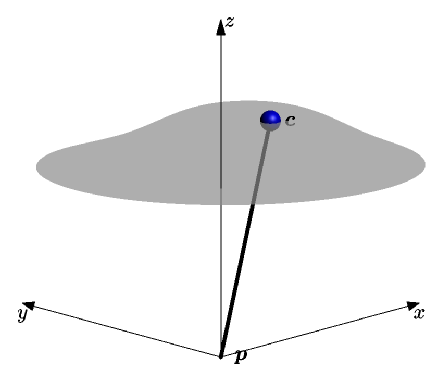
\includegraphics{inverted_pendulum.eps}}
        \caption{Inverted pendulum with a mass $\V{c}$ constrained to a plane.}
        \label{fig.inverted_pendulum1}
    \end{minipage}
    \hfill
    \begin{minipage}[t]{0.45\textwidth}
        \centering{%
        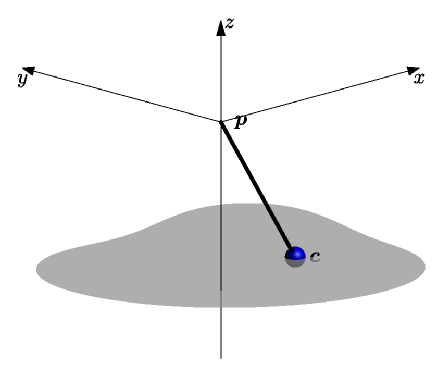
\includegraphics{pendulum.eps}}
        \caption{Pendulum with a mass $\V{c}$ constrained to a plane.}
        \label{fig.pendulum1}
    \end{minipage}
\end{figure}


Discretized version of \nameref{model.CPPMdZ} is
%
\begin{model}{PPMdZ}{Planar Point-Mass controlled with $\dot{\cop}$}
\begin{subequations}
    \begin{empheq}[left=\empheqlbrace]{align}
        &
            \V{x}_{k+1}
            =
            \begin{bmatrix}
                \tildeM{A}_k  & \M{0} \\
                \M{0}   & \tildeM{A}_k  \\
            \end{bmatrix}
            \V{x}_k
            +
            \begin{bmatrix}
                \tildeV{B}_k & \V{0}\\
                \V{0}  & \tildeV{B}_k \\
            \end{bmatrix}
            \dot{\cop}_k
            ,
            \\
        &
            \cop_{k+1}
            =
            \begin{bmatrix}
                \tildeM{D} & \M{0}\\
                \M{0} & \tildeM{D}\\
            \end{bmatrix}
            \V{x}_{k+1}
            +
            \FUNC{Z}(\zeta, \V{g}, \forceext, \momentext)
            ,
            \\[2mm]
        &
            \cop_{k+1} \in \SET{S}(\contact_{k+1,1}^{xy}, ... ,\contact_{k+1,M_s}^{xy})
            ,
    \end{empheq}
\end{subequations}
\end{model}
%
where all terms are defined as in \nameref{model.PPMJ} model, except matrices
$\tildeM{A}_k$ and $\tildeV{B}_k$, which differ depending on the sign of
$\zeta$
%
\begin{equation}
    \zeta
    =
    \frac{m (c^z - \contactC^z)}{- m \C{g}^z - \forceextC^z}.
\end{equation}
%
Note that we already have $\zeta \ne 0$ due to \cref{ass.nonzero_com_height}.
%
\begin{itemize}
    \item The variable $\zeta$ is negative, when $c^z - \contactC^z > 0$ and $-
        m \C{g}^z < \forceextC^z$, or $c^z - \contactC^z < 0$ and $- m \C{g}^z
        > \forceextC^z$. This is possible in two cases: ({\bf i}) the \ac{CoM}
        is below the support surface and $\forceextC^z$ does not cancel the
        gravity, ({\bf ii}) the \ac{CoM} is above the support surface and
        $\forceextC^z$ cancels the gravity. In any case, the robot is hanging
        and its dynamics resembles dynamics of a standard pendulum shown in
        \cref{fig.pendulum1}. We are not aware of publications, where this
        version of the model was employed, but it may be useful in some
        settings, for example, to realize locomotion on monkey bars as in
        \cite{Dai2014humanoids}, which relies on a nonlinear model. So,
        whenever $\zeta < 0$, the matrices are defined as
        \vspace{-\parskip}\par
        %
        {
        \small
        \begin{equation}
            \label{eq.ppmdz_matrices1}
            \tildeM{A}_k
            =
            \begin{bmatrix}
                1   &   \sin \left(\frac{T_k}{\sqrt{ \NORM{\zeta}}}\right) \sqrt{ \NORM{\zeta}}  &   \zeta\cos \left(\frac{T_k}{\sqrt{ \NORM{\zeta}}}\right) - \zeta \\
                0   &   \cos \left(\frac{T_k}{\sqrt{ \NORM{\zeta}}}\right)   &   \sin \left(\frac{T_k}{\sqrt{ \NORM{\zeta}}}\right) \sqrt{ \NORM{\zeta}} \\
                0   &   -\frac{1}{\sqrt{\NORM{\zeta}}} \sin \left(\frac{T_k}{\sqrt{ \NORM{\zeta}}}\right)   &   \cos \left(\frac{T_k}{\sqrt{ \NORM{\zeta}}}\right) \\
            \end{bmatrix}
            ,
            \enspace
            \tildeM{B}_k
            =
            \begin{bmatrix}
                T_k - \sin \left(\frac{T_k}{\sqrt{ \NORM{\zeta}}}\right) \sqrt{ \NORM{\zeta}} \\
                1 - \cos \left(\frac{T_k}{\sqrt{ \NORM{\zeta}}}\right) \\
                \frac{1}{\sqrt{\NORM{\zeta}}} \sin \left(\frac{T_k}{\sqrt{ \NORM{\zeta}}}\right)\\
            \end{bmatrix}
            .
        \end{equation}
        }
        %

    \item In the case of positive $\zeta$, which corresponds to \ac{LIPM}
        (\cref{fig.inverted_pendulum1}), the matrices have the following form
        %
        \begin{equation}
            \label{eq.ppmdz_matrices2}
            \tildeM{A}_k
            =
            \begin{bmatrix}
                1   &   \sinh \left(\frac{T_k}{\sqrt{\zeta}}\right) \sqrt{\zeta} &   \zeta\cosh \left(\frac{T_k}{\sqrt{\zeta}}\right) - \zeta \\
                0   &   \cosh \left(\frac{T_k}{\sqrt{\zeta}}\right)  &   \sinh \left(\frac{T_k}{\sqrt{\zeta}}\right) \sqrt{\zeta} \\
                0   &   \frac{1}{\sqrt{\zeta}}\sinh \left(\frac{T_k}{\sqrt{\zeta}}\right)     &   \cosh \left(\frac{T_k}{\sqrt{\zeta}}\right)\\
            \end{bmatrix}
            ,
            \quad
            \tildeM{B}_k
            =
            \begin{bmatrix}
                T_k - \sinh \left(\frac{T_k}{\sqrt{\zeta}}\right) \sqrt{\zeta} \\
                1 - \cosh \left(\frac{T_k}{\sqrt{\zeta}}\right) \\
                - \frac{1}{\sqrt{\zeta}} \sinh \left(\frac{T_k}{\sqrt{\zeta}}\right)
            \end{bmatrix}
            .
        \end{equation}
        %
        Note that substitution of negative $\zeta$ in the obtained matrices
        yields \cref{eq.ppmdz_matrices1}, hence, they are expressed in
        \cref{eq.ppmdz_matrices2} in a more general form.
\end{itemize}
%




%%%%%%%%%%%%%%%%%%%%%%%%%%%%%%%%%%%%%%%%%%%%%%%%%%%%%%%%%%%%%%%%%%%%%%%%%%%%%%%%
\subsection{Point-mass model with nonplanar CoM motion}

Discretization of \nameref{model.CNPM} model presented in
\cref{sec.point_mass_nonplanar} is trivial as in the case of
\nameref{model.CPPMJ} model with planar \ac{CoM} motion (see
\cref{sec.point_mass_planar_discret_jerk}).



%%%%%%%%%%%%%%%%%%%%%%%%%%%%%%%%%%%%%%%%%%%%%%%%%%%%%%%%%%%%%%%%%%%%%%%%%%%%%%%%
\subsection{Variation of discrete-time models with time}\label{sec.discret_variation}

One can observe that state transition matrices, control matrices, and
constraints in discrete-time models can be chosen differently depending on the
sampling interval $k$. Hence, some parameters of the models, which were assumed
to be constant in continuous-time case, can vary in discrete-time case if their
changes are known in advance and synchronized with the boundaries of sampling
intervals. For example,
%
\begin{itemize}
    \item The number and positions of contacts can be changed in momenta-based
        model as hinted in \cref{sec.momenta_model_discret}. Therefore, this
        model can be used to realize locomotion \cite{Nagasaka2012,
        Audren2014iros}.

    \item Variation of the discrete-time models with planar \ac{CoM} motion is
        used to change foot contacts and orientations of the feet without
        compromising linearity \cite{Herdt2010auro},
        \cref{sec.mpc_foot_positions}.

    \item The point-mass model with nonplanar \ac{CoM} motion can be utilized
        for walking on an uneven terrain, if height of the contact surface
        $\contactC^z_k$ as well as its orientation are changed appropriately
        \cite{Brasseur2015humanoids}.
\end{itemize}
%


Variation of the discrete-time models is typically realized with the help of
external routines with respect to \ac{MPC}. For example, a preliminary \ac{MPC}
problem is solved in \cite[Chapter~2]{Herdt2012thesis} to determine
orientations of the foot contacts. In the same work, a \ac{FSM} is used to set
durations and alternation of left and right foot contacts during a regular
walk. Though durations of the contacts are usually decided externally when
approximate models are employed, in some settings this can be partially avoided
with the help of motion anticipation and task prioritization as described in
\cref{sec.optional_force} and \cite{Sherikov2015humanoids}.



%%%%%%%%%%%%%%%%%%%%%%%%%%%%%%%%%%%%%%%%%%%%%%%%%%%%%%%%%%%%%%%%%%%%%%%%%%%%%%%%
%%%%%%%%%%%%%%%%%%%%%%%%%%%%%%%%%%%%%%%%%%%%%%%%%%%%%%%%%%%%%%%%%%%%%%%%%%%%%%%%
%%%%%%%%%%%%%%%%%%%%%%%%%%%%%%%%%%%%%%%%%%%%%%%%%%%%%%%%%%%%%%%%%%%%%%%%%%%%%%%%
\section{Capturability constraints}\label{sec.approx_models_capturability}

We claimed in \cref{sec.balance_general} that balance is maintained as long as
it is possible to stop the robot, \IE, capture it, without violation of the
system constraints. A capturability constraint on the final state-control pair
$(\V{x}_N, \V{u}_{N+1})$ formalizes conditions under which the robot can be
stopped. In this regard the capturability constraint is similar to the so
called \tn{terminal constraint}, which is employed in \tn{dual-mode} \ac{MPC}
\cite{Mayne2000automatica}, \cite[Chapter~6]{Rossiter2003mpc}. In this version
of \ac{MPC} a terminal constraint is imposed at the end of the preview horizon
to make sure that the system reaches some \tn{terminal set}, where a simple
local controller can stabilize the system. Here we take a similar approach, but
we want a local controller to drive the system to \tn{any} of its statically
balanced states instead of \tn{a given desired} state. Our approach is
conceptually similar to constraining the final state-control pair to a
\tn{terminal feasible invariant set} as suggested in
\cite{Schouwenaars2006thesis}.


There are several conceptual questions regarding capturability constraints,
which we would like to address before going into details of construction of
these constraints for particular models:
%
\begin{itemize}
    \item Shouldn't we aim for stability rather than capturability? So far we
        cannot give a decisive answer. Capturability is in general less
        restrictive as indicated above. On the other hand, closed loop behavior
        of an \ac{MPC} with capturability constraints may be worse, for
        example, due to different statically balanced states being chosen on
        different control iterations.

    \item Why many applications of \ac{MPC} for balance preservation are
        successful without capturability constraints \cite{Herdt2010auro,
        Kajita2003icra} and what kind of improvements such constraints can
        bring? The answer to the first part of the question lies in the fact
        that a finite preview horizon \tn{approximates} an infinite preview
        horizon, which, in turn, guarantees viability, \IE, that the robot will
        not fall \cite{Wieber2008iros}. A capturability constraint, on the
        other hand, \tn{guarantees} capturability, \IE, the ability to stop,
        even with a finite preview horizon. Hence, an \ac{MPC} problem with
        capturability constraint is more reliable in balance preservation and
        does not need the preview horizon to be as long as in the case without
        such constraint.

    \item What is the impact of a capturability constraint on feasibility of
        the underlying optimization problem? A capturability constraint, as
        well as any other hard constraint, may cause infeasibility
        \cite[Chapter~8]{Rossiter2003mpc}, which means that the chosen model of
        the robot cannot be stopped within the chosen preview horizon. This
        infeasibility is equivalent to a conflict between tasks in whole body
        motion control reviewed in \cref{sec.wbm_control} and, thus, can be
        addressed with the same numerical tools, which are discussed in
        \cref{ch.optimization}.
\end{itemize}
%


In the following subsections we construct capturability constraints for the
approximate models introduced in \cref{sec.linear_approx_models} and
discretized in \cref{sec.approx_models_discret}. In all cases we derive
constraints assuming that
%
\begin{description}
    \item[\ass{ass.timeinvariant}] The model is time-invariant, starting from
        the end of the preview horizon, which implies, in particular, that the
        number and positions of the contacts do not change. Note that our
        capturability constraints ensure recursive feasibility of
        time-invariant systems in the same way as the usual terminal
        constraints \cite{Mayne2000automatica}.
\end{description}
%
It is also presumed that the system constraints are imposed on the final
state-control pair in addition to the derived capturability constraints.



%%%%%%%%%%%%%%%%%%%%%%%%%%%%%%%%%%%%%%%%%%%%%%%%%%%%%%%%%%%%%%%%%%%%%%%%%%%%%%%%
\subsection{Momenta-based model}\label{sec.momenta_model_capturability}
In its simplest form a capturability constraint imposes that the robot is in a
statically balanced state. A statically balanced state must necessarily be a
part of a fixed point, \IE, such state-control pair $(\V{x}_k, \V{u}_k)$ that
\cite[Chapter~8]{Scheinerman1996ids}
%
\begin{equation}
    \V{x}_k = \M{A}_k \V{x}_k + \M{B}_k \V{u}_k.
\end{equation}
%
In the case of momenta-based (\nameref{model.MB}) model, this condition results
in the following constraints, where indices of state and control variables are
omitted for simplicity:
%
\begin{itemize}
    \item $\V{\LM}^{xy} = \V{0}$ -- no linear momentum in the $x$-$y$ plane,
        \IE, the \ac{CoM} velocity is zero $\dotV{c}^{xy} = \V{0}$;

    \item $m \V{g}^{xy} + \sum_{i=1}^{M} \force_i^{xy} = \V{0}$ -- no forces in
        the $x$-$y$ plane, \IE, the \ac{CoM} acceleration is zero
        $\ddotV{c}^{xy} = \V{0}$;

    \item the rate of change of the angular momentum about the $x$ and $y$ axes
        is also zero:
        \begin{equation}
            \begin{aligned}
                \dotV[c]{\AM}^{xy}
                &=
                \begin{bmatrix}
                        \hatC{\LM}^y \C{g}^z
                        +
                        \sum_{i=1}^{M}
                        \left(
                            \forceC^z_i \contactC_i^y
                            +
                            \Ix \moment_i
                            -
                            \forceC^y_i (\contactC^z_i - \C{c}^z)
                        \right)
                    \\
                        -\hatC{\LM}^x \C{g}^z
                        +
                        \sum_{i=1}^{M}
                        \left(
                            -\forceC^z_i \contactC_i^x
                            +
                            \Iy \moment_i
                            +
                            \forceC^x_i (\contactC^z_i - \C{c}^z)
                        \right)
                \end{bmatrix}
                \\
                &=
                \begin{bmatrix}
                        \hatC{\LM}^y \C{g}^z
                        -
                        m \C{c}^z \C{g}^y
                        +
                        \sum_{i=1}^{M}
                        \left(
                            \forceC^z_i \contactC_i^y
                            +
                            \Ix \moment_i
                            -
                            \forceC^y_i \contactC^z_i
                        \right)
                    \\
                        -\hatC{\LM}^x \C{g}^z
                        +
                        m \C{c}^z \C{g}^x
                        +
                        \sum_{i=1}^{M}
                        \left(
                            - \forceC^z_i \contactC_i^x
                            +
                            \Iy \moment_i
                            +
                            \forceC^x_i \contactC^z_i
                        \right)
                \end{bmatrix}
                =
                \V{0}.
            \end{aligned}
        \end{equation}
\end{itemize}
%
Note that the fixed points of the approximate system include states with
non-zero angular momentum $\V[c]{\AM}^{xy} \neq \V{0}$, even though the real
system cannot store angular momentum \cite{Stephens2010iros}. Consequently, a
fixed point of this approximate model does not always correspond to a fixed
point of the whole body model and does not imply that the latter is captured.
We alleviate this issue by imposing that $\V[c]{\AM}^{xy}$ is zero as well.
Furthermore, provided that $m \V{g}^{xy} + \sum_{i=1}^{M} \force_i^{xy} =
\V{0}$ holds, we can also determine $\dotC[c]{\AM}^{z}$ using the equation
\cref{eq.component_wise_momenta} and constrain it:
%
\begin{equation}
    \begin{aligned}
        \dotC[c]{\AM}^z
        &=
        \sum_{i=1}^M
        \left(
            \begin{bmatrix}
                - (\contactC_i^y - {c}^y) & \contactC_i^x - {c}^x       & 0
            \end{bmatrix}
            \force_i
            +
            \Iz
            \moment_i
        \right)
        \\
        & =
        \sum_{i=1}^M
        \left(
            \contactC_i^x
            \forceC_i^y
            -
            \contactC_i^y
            \forceC_i^x
            +
            \Iz
            \moment_i
        \right)
        +
        \hatC{\LM}^x
        \C{g}^y
        -
        \hatC{\LM}^y
        \C{g}^x
        =
        0
        ,
    \end{aligned}
\end{equation}
%
even though $\dotC[c]{\AM}^z$ depends nonlinearly on the state and control
variables in general.


Thus, the complete capturability constraint is defined as
%
\begin{subequations}
    \label{eq.capture_momenta_model}
    \begin{empheq}[left=\empheqlbrace]{alignat=2}
        &\V{\LM}^{xy}
        &&= \V{0},
        \\
        &\V[c]{\AM}^{xy}
        &&= \V{0},
        \\
        &\dotV{\LM}^{xy}
        &&= m \V{g}^{xy} + \sum_{i=1}^{M} \force_i^{xy} = \V{0},
        \\
        &
        \dotV[c]{\AM}
        &&=
        -
        \V{g}
        \CROSS
        \begin{bmatrix}
            \hatV{\LM}^{xy}\\
            m \C{c}^z
        \end{bmatrix}
        +
        \sum_{i=1}^{M}
        \left(
            \contact_i
            \CROSS
            \force_i
            +
            \moment_i
        \right)
        =
        \V{0}
        .
    \end{empheq}
\end{subequations}
%
Note that the capturability constraint imposed in \cite{Sherikov2015humanoids}
for the same model is not entirely correct.



%%%%%%%%%%%%%%%%%%%%%%%%%%%%%%%%%%%%%%%%%%%%%%%%%%%%%%%%%%%%%%%%%%%%%%%%%%%%%%%%
\subsection{Point-mass models with planar CoM motion}\label{sec.point_mass_planar_capturability}

In the present section we construct capturability constraints for the two third
order point-mass models introduced in \cref{sec.point_mass_planar} and
discretized in \cref{sec.point_mass_planar_discret}. We approach the derivation
of these constraints using the idea of dual-mode \ac{MPC} instead of
identification of fixed points as in the previous case of the momenta-based
model. To be more precise, we use capturability constraints to specify a set of
states, starting from which the system can converge to a statically balanced
state with the help of a simple linear feedback controller. Strictly speaking,
\tn{convergence} to a statically balanced state contradicts with our definition
of capturability given in \cref{ch.balance}, since this definition requires
that the system reaches a statically balanced state in \tn{finite} time.
However, we consider this contradiction to be insignificant.


We construct linear feedback controllers in such a way, that they maintain a
constant position of the \ac{CoP}. This implies that constraints on this
position will not be violated in the future. Though the controllers are
supposed to be discrete-time, we consider their continuous-time counterparts as
well to emphasize relations and differences between variants of the model with
different control variables.


In order to simplify presentation, we exploit the fact, that the state
transition and control matrices in systems are block diagonal and each block
corresponds to motion along the $x$ or $y$ axis. This allows us to limit our
analysis to blocks $\tildeM{A}$, $\tildeV{B}$, $\tildeM{A}_k$, $\tildeV{B}_k$
defined in \cref{sec.point_mass_planar,sec.point_mass_planar_discret}
respectively.



%%%%%%%%%%%%%%%%%%%%%%%%%%%%%%%%%%%%%%%%%%%%%%%%%%%%%%%%%%%%%
\subsubsection{Continuous-time model controlled by the CoM jerk}

In this section we work with \nameref{model.CPPMJ} model. Our goal is to derive
a controller, which maintains constant position of the \ac{CoP} or, in other
words, maintains zero velocity of the \ac{CoP}. Velocity of the \ac{CoP} can be
found by differentiation of the equation \cref{eq.point_mass_jerk_control.cop}
(assuming constant external wrench $(\forceext, \momentext)$):
%
\begin{equation}
    \dot{\cop} = \dotV{c}^{xy} - \zeta \dddotV{c}^{xy} = \V{0}.
\end{equation}
%
If $\zeta = 0$, the \ac{CoP} velocity is zero when the \ac{CoM} velocity is
zero. Hence, the capturability constraint is
%
\begin{equation}
    \dotV{c}^{xy} = \V{0}
    ,
    \quad
    \ddotV{c}^{xy} = \V{0}
    ,
    \quad
    \dddotV{c}^{xy} = \V{0}.
\end{equation}
%
If $\zeta \ne 0$, we substitute $\dddotV{c}^{xy} = \dotV{c}^{xy} / \zeta$ into
the model. The obtained model is identical to \nameref{model.CPPMdZ} model with
control input equal to zero $\dot{\cop} = \V{0}$. This case is analyzed in the
following subsection, while the discrete-time case of the model controlled by
the \ac{CoM} jerk is considered afterwards.


%%%%%%%%%%%%%%%%%%%%%%%%%%%%%%%%%%%%%%%%%%%%%%%%%%%%%%%%%%%%%
\subsubsection{Continuous and discrete-time models controlled by the CoP velocity}\label{sec.capturability_cop_control}

Position of the \ac{CoP} in \nameref{model.CPPMdZ} model can always be
maintained with a trivial linear controller $\dot{\cop} = \V{0}$. Hence, we can
analyze stability of the system with the help of eigen decomposition of the
state transition matrices $\tildeM{A}$ and $\tildeM{A}_k$
%
\begin{equation}
    \tildeM{A}
    =
    \begin{bmatrix}
        0   &  1  &   0 \\
        0   &  0  &  1 \\
        0   &  \frac{1}{\zeta}   &  0   \\
    \end{bmatrix}
    ,
    \quad
    \tildeM{A}_k
    =
    \begin{bmatrix}
        1   &   \sinh \left(\frac{T_k}{\sqrt{\zeta}}\right) \sqrt{\zeta} &   \zeta\cosh \left(\frac{T_k}{\sqrt{\zeta}}\right) - \zeta \\
        0   &   \cosh \left(\frac{T_k}{\sqrt{\zeta}}\right)  &   \sinh \left(\frac{T_k}{\sqrt{\zeta}}\right) \sqrt{\zeta} \\
        0   &   \frac{1}{\sqrt{\zeta}}\sinh \left(\frac{T_k}{\sqrt{\zeta}}\right)     &   \cosh \left(\frac{T_k}{\sqrt{\zeta}}\right)\\
    \end{bmatrix}
    .
\end{equation}
%
Eigen decomposition allows to identify unstable eigenvalues and nullify
unstable modes of the system \cite{Scheinerman1996ids, Muske1993aiche}.
Eigenvalues of matrices $\tildeM{A}$ and $\tildeM{A}_k$ are
%
\begin{equation}
    \left(-\frac{1}{\sqrt{\zeta}}, \frac{1}{\sqrt{\zeta}}, 0 \right)
    \mbox{ and }
    \left( e^{-\frac{T_k}{\sqrt{\zeta}}}, e^{\frac{T_k}{\sqrt{\zeta}}}, 1 \right)
\end{equation}
respectively, where $e$ is Euler's number. Thus, stability of the systems is
determined by the sign of $\zeta$
%
\begin{itemize}
    \item When $\zeta < 0$ matrix $\tildeM{A}$ has two purely imaginary and one
        zero eigenvalues. In order to suppress oscillatory behavior in this
        case it is necessary to set the \ac{CoM} velocities and accelerations
        to zero:
        %
        \begin{equation}
            \dotV{c}^{xy} = \V{0}
            ,
            \quad
            \ddotV{c}^{xy} = \V{0}.
        \end{equation}
        %
        Analysis of the discrete-time matrix $\tildeM{A}_k$ results in the same
        conclusion.

    \item If, on the opposite, $\zeta > 0$, matrix $\tildeM{A}$ has one
        unstable positive, one negative and one zero eigenvalues. The unstable
        mode is nullified when
        %
        \begin{equation}\label{eq.cop_control_capturability_ctr}
            \dotV{c}^{xy} + \sqrt{\zeta} \ddotV{c}^{xy} = \V{0}.
        \end{equation}
        %
        If this equation holds, the system with zero input converges to a fixed
        point with $\V{c}^{xy} = \cop$, $\dotV{c}^{xy} = \V{0}$, and
        $\ddotV{c}^{xy} = \V{0}$. The same is true for the discrete-time
        system.
\end{itemize}
%
Note that due to \cref{eq.cop_control_capturability_ctr}
%
\begin{equation}
    \dot{\cp} = \dotV{c}^{xy} + \sqrt{\zeta} \dddotV{c}^{xy} = \V{0},
\end{equation}
%
where $\cp$ is the \tn{capture point}, which is defined as the point on the
ground where the robot should step to stop \cite{Koolen2012ijrr,
Takenaka2009iros, Englsberger2011iros, Hof2005job}. In our case $\cp$ is the
position of the \ac{CoP}, which lies within the support area and to which
$\V{c}^{xy}$ converges. The capturability constraint
\cref{eq.cop_control_capturability_ctr} ensures that this point does not move,
which is implied in the other works where the second order model is considered
\cite{Koolen2012ijrr, Englsberger2011iros}.



%%%%%%%%%%%%%%%%%%%%%%%%%%%%%%%%%%%%%%%%%%%%%%%%%%%%%%%%%%%%%
\subsubsection{Discrete-time model controlled by the CoM jerk}

In the case of the discrete-time version of \nameref{model.CPPMJ} model our
goal is to construct controller such that $\cop_k = \cop_{k+1}$ and
%
\begin{equation}
    \label{eq.ppmj_cop_diff}
    \cop_k
    -
    \cop_{k+1}
    =
    \tildeM{D}
    \begin{bmatrix}
        \C{c}^\alpha_k\\
        \dotC{c}^\alpha_k\\
        \ddotC{c}^\alpha_k
    \end{bmatrix}
    -
    \tildeM{D}
    \left(
        \tildeM{A}_k
        \begin{bmatrix}
            \C{c}^\alpha_k\\
            \dotC{c}^\alpha_k\\
            \ddotC{c}^\alpha_k
        \end{bmatrix}
        +
        \tildeV{B}_k
        \dddotC{c}^{\alpha}_k
    \right)
    =
    0
    ,
\end{equation}
%
where $\alpha \in \{x,y\}$. When $\tildeM{D}\tildeV{B}_k = 0$ this equation is
satisfied if $\dotC{c}^\alpha_k = 0$ and $\ddotC{c}^\alpha_k = 0$. Otherwise,
we can find $\dddotC{c}^{\alpha}_k$ from \cref{eq.ppmj_cop_diff} and substitute
it into the equation of dynamics of the system to obtain a new state transition
matrix
%
\begin{equation}
    \left(
        \tildeM{A}_k
        +
        \tildeV{B}_k
        {
        \left(
            \tildeM{D}
            \tildeV{B}_k
        \right)
        }^{-1}
        \tildeM{D}
        \left(
            \V{I}_{3,3}
            -
            \tildeM{A}_k
        \right)
    \right)
    ,
\end{equation}
%
whose eigenvalues are
%
\begin{equation}
    \left(
        \frac{\sqrt{3} T_k \sqrt{12 \zeta + T_k^2} + 6 \zeta + 2 T_k^2}{6 \zeta - T_k^2}
        ,
        \frac{ - \sqrt{3} T_k \sqrt{12 \zeta + T_k^2} + 6 \zeta + 2 T_k^2}{6 \zeta - T_k^2}
        ,
        1
    \right).
\end{equation}
%
We do not go further in the analysis due to subtle dependence of the
eigenvalues on parameters $\zeta$ and $T_k$. When the parameters are known,
appropriate constraints can be easily found. These constraints, however, are
not the same as in the case of continuous-time version of this system.
Alternatively, it is possible to explicitly impose a complete stop with
%
\begin{equation}
    \dotV{c}^{xy} = \V{0}
    ,
    \quad
    \ddotV{c}^{xy} = \V{0}
    ,
    \quad
    \dddotV{c}^{xy} = \V{0}
    ,
\end{equation}
%


%%%%%%%%%%%%%%%%%%%%%%%%%%%%%%%%%%%%%%%%%%%%%%%%%%%%%%%%%%%%%%%%%%%%%%%%%%%%%%%%
\subsection{Point-mass model with nonplanar CoM motion}

A simple linear controller capable of stopping the system without violation of
the constraints does not seem to exist. Therefore, we do not use the same
approach for derivation of the capturability constraint as in
\cref{sec.point_mass_planar_capturability}, instead, we suggest to explicitly
stop the \ac{CoM} motion with
%
\begin{equation}
    \dotV{c} = \V{0}
    ,
    \quad
    \ddotV{c} = \V{0}
    ,
    \quad
    \dddotV{c} = \V{0}.
\end{equation}
%


%%%%%%%%%%%%%%%%%%%%%%%%%%%%%%%%%%%%%%%%%%%%%%%%%%%%%%%%%%%%%%%%%%%%%%%%%%%%%%%%
\subsection{Infeasibility due to variation of a model with time}

We have already briefly discussed infeasibility of the capturability
constraints in the introduction of this section. In the conclusion we would
like to point out a particular type of infeasibility, which is caused by
variation of models with time (see \cref{sec.discret_variation}).


Consider a situation, when the model changes in the very end of the preview
horizon due to a change in the contact stance. It is usually impossible to
change the contact stance and completely stop within the same final sampling
interval, since these goals overconstrain the final control input. This issue,
however, is not observed in the case of the point-mass model with planar
\ac{CoM} motion when convergence to a statically balanced state is exploited
(see \cref{sec.capturability_cop_control}). In other cases, various heuristics
can be employed to avoid infeasibility of the capturability constraint.




%%%%%%%%%%%%%%%%%%%%%%%%%%%%%%%%%%%%%%%%%%%%%%%%%%%%%%%%%%%%%%%%%%%%%%%%%%%%%%%%
%%%%%%%%%%%%%%%%%%%%%%%%%%%%%%%%%%%%%%%%%%%%%%%%%%%%%%%%%%%%%%%%%%%%%%%%%%%%%%%%
%%%%%%%%%%%%%%%%%%%%%%%%%%%%%%%%%%%%%%%%%%%%%%%%%%%%%%%%%%%%%%%%%%%%%%%%%%%%%%%%
\section{Point-mass model with foot motion}\label{sec.walkmodel}

We do not employ any of the point-mass models presented in
\cref{sec.approx_models_discret} for walking \tn{per se}, but rather an
augmented version of \nameref{model.PPMdZ} model. The augmented version
includes a linear system, which reflects changes of positions of the feet on
the ground in the preview horizon as in \cite{Herdt2010auro}. For the sake of
computational performance all inequality constraints in the augmented version
are expressed as simple bounds (see \cref{sec.simple_bounds}).


%%%%%%%%%%%%%%%%%%%%%%%%%%%%%%%%%%%%%%%%%%%%%%%%%%%%%%%%%%%%%%%%%%%%%%%%%%%%%%%%
\subsection{Modeling of changes of the foot positions}\label{sec.mpc_foot_positions}

We model changes of the foot positions on the ground in order to facilitate
their automatic adjustment, which allows for disturbance compensation and
tracking of desired walking speed \cite{Herdt2010auro}. Future foot positions
can be found using the following discrete-time linear system
%
\begin{subequations}\label{eq.foot_model}
    \begin{empheq}[left=\empheqlbrace]{align}
        &
            \hat{\contact}_{j+1}
            =
            \hat{\contact}_{j}
            +
            \hatM[j][]{R}
            \Delta\hat{\contact}_{j}
            ,
            \quad
            j
            \in
            \{0, ..., K-1\}
            ,
            \\
        &
            \Delta\hat{\contact}_{j} \in \SET{F}_j
            ,
    \end{empheq}
\end{subequations}
%
where $\Delta\hat{\contact}_{j}$ is the distance between the $j$-th and $j+1$
foot positions expressed in frame $\FRAME{j}$ fixed to $j$-th foot,
$\hatM[j][]{R}$ transforms $\Delta\hat{\contact}_{j}$ to the global frame, and
$\SET{F}_j$ defines a polygonal area of allowed positions of
$\hat{\contact}_{j+1}$ with respect to $\hat{\contact}_{j}$
\cite{Stasse2009Humanoids,Herdt2010auro}. $K$ is the number of adjustable foot
positions in the preview horizon. $\hat{\contact}_{0}$ denotes the current
support foot position and is, therefore, fixed.


Combination of \cref{eq.foot_model} with \nameref{model.PPMdZ} model gives
%
\begin{subequations}
    \begin{empheq}[left=\empheqlbrace]{align}
        &
            \V{x}_{k+1}
            =
            \begin{bmatrix}
                \tildeM{A}_k  & \M{0} \\
                \M{0}   & \tildeM{A}_k  \\
            \end{bmatrix}
            \V{x}_k
            +
            \begin{bmatrix}
                \tildeV{B}_k & \V{0}\\
                \V{0}  & \tildeV{B}_k \\
            \end{bmatrix}
            \dot{\cop}_k
            ,
            &&
            k
            \in
            \{0, ..., N-1\}
            ,
            \\
        &
            \hat{\contact}_{j+1}
            =
            \hat{\contact}_{j}
            +
            \hatM[j][]{R}
            \Delta\hat{\contact}_{j}
            ,
            &&
            j
            \in
            \{0, ..., K-1\}
            ,
            \\[2mm]
        &
            \cop_{k+1}
            =
            \begin{bmatrix}
                \tildeM{D} & \M{0}\\
                \M{0} & \tildeM{D}\\
            \end{bmatrix}
            \V{x}_{k+1}
            ,
            \\
        &
            (\contact_{k+1,1}^{xy}, ..., \contact_{k+1,M_s}^{xy}) = \FUNC{F}_{k+1}(\hat{\contact}_{0}, ..., \hat{\contact}_{K})
            ,
            \\[2mm]
        &
            \Delta\hat{\contact}_{j} \in \SET{F}_j
            ,
            \\
        &
            \cop_{k+1} \in \SET{S}(\contact_{k+1,1}^{xy}, ..., \contact_{k+1,M_s}^{xy})
            ,
    \end{empheq}
\end{subequations}
%
where the function $\FUNC{F}_{k+1}$ selects foot positions at the instant
$k+1$. Here we assumed that the gravity vector is aligned with the $z$ axis and
there is no external wrench acting on the model, \IE, $\FUNC{Z}(\zeta, \V{g},
\forceext, \momentext) = \V{0}$. We indicated in \cref{sec.surface_contacts}
that the constraints on the position of \ac{CoP} during double supports depend
nonlinearly on foot positions (see \cref{sec.surface_contacts}). In order to
avoid this nonlinearity, we impose the \ac{CoP} constraints only when the
system is in single support \cite{Herdt2010auro}, or approximate double support
constraints with single support constraints as explained in
\cref{sec.surface_contacts}. In either case the number of contacts $M_s = 1$,
and the model is simplified to
%
\begin{subequations}\label{eq.foot_model2}
    \begin{empheq}[left=\empheqlbrace]{align}
        &
            \V{x}_{k+1}
            =
            \begin{bmatrix}
                \tildeM{A}_k  & \M{0} \\
                \M{0}   & \tildeM{A}_k  \\
            \end{bmatrix}
            \V{x}_k
            +
            \begin{bmatrix}
                \tildeV{B}_k & \V{0}\\
                \V{0}  & \tildeV{B}_k \\
            \end{bmatrix}
            \dot{\cop}_k
            ,
            &&
            k
            \in
            \{0, ..., N-1\}
            ,
            \\
        &
            \hat{\contact}_{j+1}
            =
            \hat{\contact}_{j}
            +
            \hatM[j][]{R}
            \Delta\hat{\contact}_{j}
            ,
            &&
            j
            \in
            \{0, ..., K-1\}
            ,
            \\[2mm]
        &
            \cop_{k+1}
            =
            \begin{bmatrix}
                \tildeM{D} & \M{0}\\
                \M{0} & \tildeM{D}\\
            \end{bmatrix}
            \V{x}_{k+1}
            ,
            \\
        &
            \contact_{k+1}^{xy} = \FUNC{F}_{k+1}(\hat{\contact}_{0}, ..., \hat{\contact}_{K})
            ,
            \\[2mm]
        &
            \Delta\hat{\contact}_{j} \in \SET{F}_j
            ,
            \\
        &
            \cop_{k+1} \in \SET{S}(\contact_{k+1}^{xy})
            ,
    \end{empheq}
\end{subequations}
%



%%%%%%%%%%%%%%%%%%%%%%%%%%%%%%%%%%%%%%%%%%%%%%%%%%%%%%%%%%%%%%%%%%%%%%%%%%%%%%%%
\subsection{Conversion of the constraints to simple bounds}\label{sec.mpc_simple_bounds}

Constraints on the \ac{CoP} positions are expressed as simple bounds in frames
fixed to the feet provided that the feet are rectangular (see
\cref{sec.surface_contacts}). Hence, we redefine the output of the system
\cref{eq.foot_model2} as follows:
%
\begin{equation}
    \hat{\cop}_{k+1}
    =
    \M[][k+1]{R}
    \left(
        \begin{bmatrix}
            \tildeM{D} & \M{0}\\
            \M{0} & \tildeM{D}\\
        \end{bmatrix}
        \V{x}_{k+1}
        -
        \contact_{k+1}^{xy}
    \right)
    ,
\end{equation}
%
where $\M[][k+1]{R}$ is the rotation matrix representing orientation of the foot
at instant $k+1$. Then constraints on the \ac{CoP} position are changed to
%
\begin{equation}
    \underbrace{
        -
        \begin{bmatrix}
            w\\
            \ell\\
        \end{bmatrix}
    }_{\ubar{\cop}}
    \le
    \hat{\cop}_{k+1}
    \le
    \underbrace{
        \begin{bmatrix}
            w\\
            \ell\\
        \end{bmatrix}
    }_{\bar{\cop}}
    ,
\end{equation}
%
where $2w$ and $2\ell$ are the width and the length of the foot sole
(\cref{sec.rectangular_foot}).


The structure of the constraints on the \ac{CoP} positions is lost after
condensing of the \ac{MPC} problem as described in \cref{app.condensing}. We
avoid this by changing the control inputs of the model to $\hat{\cop}_{k+1}$.
For this purpose we reformulate the output equation again
%
\begin{equation}
    \begin{split}
        \hat{\cop}_{k+1}
        &=
        \M[][k+1]{R}
        \left(
            \begin{bmatrix}
                \tildeM{D} & \M{0}\\
                \M{0} & \tildeM{D}\\
            \end{bmatrix}
            \V{x}_{k+1}
            -
            \contact_{k+1}^{xy}
        \right)\\
        &=
        \M[][k+1]{R}
        \left(
            \begin{bmatrix}
                \tildeM{D} & \M{0}\\
                \M{0} & \tildeM{D}\\
            \end{bmatrix}
            \V{x}_{k}
            +
            T_k \dot{\cop}_k
            -
            \contact_{k+1}^{xy}
        \right)
        ,
    \end{split}
\end{equation}
%
then find $\dot{\cop}_k$ using it
%
\begin{equation}
    \dot{\cop}_k
    =
    \underbrace{
        -
        \frac{1}{T_k}
        \begin{bmatrix}
            \tildeM{D} & \M{0}\\
            \M{0} & \tildeM{D}\\
        \end{bmatrix}
    }_{\M{D}_k}
    \V{x}_{k}
    +
    \underbrace{
        \frac{1}{T_k}
        \begin{bmatrix}
            \M[k+1][]{R} & \M{I}_2 \\
        \end{bmatrix}
    }_{\M{E}_k}
    \begin{bmatrix}
        \hat{\cop}_{k+1}\\
        \contact_{k+1}^{xy}
    \end{bmatrix}
    ,
\end{equation}
%
and substitute it in the equation of dynamics of the system
%
\begin{equation}
    \begin{aligned}
    \V{x}_{k+1}
    &=
    \begin{bmatrix}
        \tildeM{A}_k  & \M{0} \\
        \M{0}   & \tildeM{A}_k  \\
    \end{bmatrix}
    \V{x}_k
    +
    \frac{1}{T_k}
    \begin{bmatrix}
        \tildeV{B}_k & \V{0}\\
        \V{0}  & \tildeV{B}_k \\
    \end{bmatrix}
    \left(
        -
        \begin{bmatrix}
            \tildeM{D} & \M{0}\\
            \M{0} & \tildeM{D}\\
        \end{bmatrix}
        \V{x}_{k}
        +
        \M[k+1][]{R} \hat{\cop}_{k+1}
        +
        \contact_{k+1}^{xy}
    \right)
    \\
    & =
    \underbrace{
        \begin{bmatrix}
            \tildeM{A}_k - \frac{1}{T_k} \tildeV{B}_k \tildeM{D}  & \M{0} \\
            \M{0}   & \tildeM{A}_k - \frac{1}{T_k} \tildeV{B}_k \tildeM{D} \\
        \end{bmatrix}
    }_{\M{A}_k}
    \V{x}_k
    +
    \underbrace{
        \begin{bmatrix}
            \frac{1}{T_k}\tildeV{B}_k & \V{0}\\
            \V{0}  & \frac{1}{T_k}\tildeV{B}_k \\
        \end{bmatrix}
        \begin{bmatrix}
            \M[k+1][]{R} \M{I}_2 \\
        \end{bmatrix}
    }_{\M{B}_k}
    \begin{bmatrix}
        \hat{\cop}_{k+1}\\
        \contact_{k+1}^{xy}
    \end{bmatrix}
    .
    \\
    \end{aligned}
\end{equation}
%


Constraints on the foot positions are also expressed as simple bounds on
$\Delta\hat{\contact}_{j}$ provided that $\SET{F}_j$ defines a rectangular
area. In this case the model of the system takes the following form
%
\begin{model}{PPMZ}{Planar Point-Mass controlled with \acs{CoP} position}
\begin{subequations}
    \begin{empheq}[left=\empheqlbrace]{align}
        &
            \V{x}_{k+1}
            =
            \M{A}_k
            \V{x}_k
            +
            \M{B}_k
            \begin{bmatrix}
                \hat{\cop}_{k+1}\\
                \contact_{k+1}^{xy}
            \end{bmatrix}
            ,
            &&
            k
            \in
            \{0, ..., N-1\}
            ,
            \\
        &
            \hat{\contact}_{j+1}
            =
            \hat{\contact}_{j}
            +
            \hatM{B}_j
            \Delta\hat{\contact}_{j}
            ,
            &&
            j
            \in
            \{0, ..., K-1\}
            ,
            \\[2mm]
        &
            \dot{\cop}_k
            =
            \M{D}_k
            \V{x}_{k}
            +
            \M{E}_k
            \begin{bmatrix}
                \hat{\cop}_{k+1}\\
                \contact_{k+1}^{xy}
            \end{bmatrix}
            ,
            \\
        &
            \contact_{k+1}^{xy} = \FUNC{F}_{k+1}(\hat{\contact}_{0}, ..., \hat{\contact}_{K})
            ,
            \\[2mm]
        &
            \ubarV{\objb}_{\contact,j} \le \Delta\hat{\contact}_{j}^{xy} \le \barV{\objb}_{\contact,j}
            ,
            \\
        &   \ubar{\cop} \le \hat{\cop}_{k+1} \le \bar{\cop}
            ,
    \end{empheq}
\end{subequations}
\end{model}
%
Note that the structure of simple bounds on $\Delta\hat{\contact}_{1,...,K}$ is
also lost after condensing. In order to avoid this it is necessary to express
$\contact_{1,...,N}^{xy}$ using $\Delta\hat{\contact}_{1,...,K}$ after
condensing.


%%%%%%%%%%%%%%%%%%%%%%%%%%%%%%%%%%%%%%%%%%%%%%%%%%%%%%%%%%%%%%%%%%%%%%%%%%%%%%%%
\subsection{Motion of the feet in the air}\label{sec.mpc_feet_trajectories}

\nameref{model.PPMZ} model accounts for foot positions on the ground, but
neglects motion of the feet in the air. We use $3$-rd order polynomials to
represent this motion \cite{Sherikov2014humanoids, Nishiwaki2009ijrr}. Hence,
acceleration of the foot in the air at a given control instant is found using a
linear function of $\Delta\hat{\contact}_{0}$:
%
\begin{equation}
    \ddotV{s}_{0}
    =
    \objA_{\MT{sa}}
    \Delta\hat{\contact}_{0}
    +
    \V{\objb}_{\MT{sa}},
\end{equation}
%
where $\objA_{\MT{sa}}$ and $\V{\objb}_{\MT{sa}}$ are constructed as described
in \cref{app.swing_foot}. In a similar way we find $x$ and $y$ components of
the foot jerk
%
\begin{equation}
    \dddotV{s}^{xy}
    =
    \objA_{\MT{sj}}
    \Delta\hat{\contact}_{0}
    +
    \V{\objb}_{\MT{sj}}
    ,
\end{equation}
%
which is constant for the whole foot trajectory. We will use $\ddotV{s}_{0}$
and $\dddotV{s}^{xy}$ in whole body motion controllers considered in
\cref{ch.simulations}.



%%%%%%%%%%%%%%%%%%%%%%%%%%%%%%%%%%%%%%%%%%%%%%%%%%%%%%%%%%%%%%%%%%%%%%%%%%%%%%%%
%%%%%%%%%%%%%%%%%%%%%%%%%%%%%%%%%%%%%%%%%%%%%%%%%%%%%%%%%%%%%%%%%%%%%%%%%%%%%%%%
%%%%%%%%%%%%%%%%%%%%%%%%%%%%%%%%%%%%%%%%%%%%%%%%%%%%%%%%%%%%%%%%%%%%%%%%%%%%%%%%
\section{Mixed Model Predictive Control}\label{sec.mmpc}

The traditional approach to control of humanoid robots using anticipation with
approximate models is divided into two main sequential stages
\cite{Kajita2003icra, Herdt2010auro, Morisawa2007icra, Nishiwaki2009ijrr}:
%
\begin{enumerate}
    \item anticipation of trajectories of the \ac{CoM}, \ac{CoP}, momenta, or
        contact forces using \ac{MPC} or analytic formulas;

    \item tracking of the generated trajectories with a whole body motion
        controller taking into account whole body tasks and constraints.
\end{enumerate}
%
In the following this approach is referred to as \tn{two-stage control}. It has
several disadvantages:
%
\begin{itemize}
    \item As we have learned in \cref{sec.nonlinear_approx_models}, whole body
        constraints are neglected in simplified models (\cref{ass.nojointctr})
        and must be approximated with proxy constraints. Hence, the generated
        trajectories can be infeasible for the whole body model. Though an
        infeasible trajectory may still be executed approximately
        \cite{Kanehiro2009humanoids}, it is always preferable to avoid such
        situations.

    \item The whole body tasks cannot in general be expressed with an
        approximate model, and, thus, cannot be taken into account during
        anticipation without some \tn{ad hoc} task-specific techniques
        \cite{Yoshida2006humanoids, Nishiwaki2003icra, Fukumoto2004iros}.
\end{itemize}
%
In order to address these disadvantages we propose to merge the two sequential
stages into one \cite{Sherikov2014humanoids, Sherikov2015humanoids},
\cref{sec.mmpc_hierarchy}.


Here we call our approach \acf{MMPC}. It consists in using both the whole body
model and an approximate model within the same preview horizon. This approach
should not be confused with \tn{Multi-Model Predictive Control}, where the
model may differ from one \ac{MPC} iteration to another, but each preview
horizon is formed using a single model \cite[Chapter~15]{Rossiter2003mpc}.
\ac{MMPC} is also different from the \tn{Distributed Model Predictive Control},
where a complex system is broken down into several simpler interacting systems
\cite[Chapter~6]{Rawlings2009mpc}. We are not aware of previous works using
\ac{MMPC}, though conceptually similar ideas were proposed for motion planning
in \cite{Dai2014humanoids, Kanoun2010ijrr}.


We summarize advantages and limitations of \ac{MMPC} in
\cref{sec.mmpc_advantages_limitations} after discussion of some technical
details of mixing models in the preview horizon in \cref{sec.mmpc_horizon}.


%%%%%%%%%%%%%%%%%%%%%%%%%%%%%%%%%%%%%%%%%%%%%%%%%%%%%%%%%%%%%%%%%%%%%%%%%%%%%%%%
\subsection{Composition of the preview horizon}\label{sec.mmpc_horizon}

In order to avoid nonlinearity we introduce the whole body model of a robot
only at the current instant of the preview horizon, while the rest of it is
formed using an approximate model. Such combination of the models can be
interpreted as a whole body \ac{MPC}, where the whole body model is replaced by
a simplified model everywhere except the current time instant
\cite{Sherikov2015humanoids}. Alternatively, we can say that we construct a
whole body motion controller with built-in anticipation for ensuring long-term
balance \cite{Sherikov2014humanoids}.


The initial state-control pair $(\V{x}_0, \V{u}_0)$ is shared by both coupled
models. Therefore, when the whole body model is coupled with the momenta-based
(\nameref{model.MB}) model, they share initial momenta and the contact wrenches
applied on the first interval of the preview horizon $\wrench_{0,\{0, ...,
M\}}$ \cite{Sherikov2015humanoids}. Coupling with third order point-mass models
\nameref{model.PPMdZ} and \nameref{model.PPMJ} is not as trivial
\cite{Sherikov2014humanoids}:
%
\begin{itemize}
    \item The first reason for this is mismatch of the orders of models:
        accelerations are part of the state in the approximate models and are
        control variables in the whole body model. In order to alleviate this
        issue we include the initial \ac{CoM} acceleration $\ddotV{c}^{xy}_0$
        into the control vector $\V{u}_0$ rather than state $\V{x}_0$.

    \item The second problem is due to \cref{ass.point_mass}, which requires
        the rate of angular momentum to be zero in the point-mass models.
        Consequently, the same change in the \ac{CoP} position results in
        different motions of \ac{CoM} in approximate and whole body models,
        since the latter generates nonzero rate of angular momentum most of the
        time. Enforcing both the \ac{CoM} and \ac{CoP} motion of a point-mass
        model on the whole body model is infeasible or leads to unnatural and
        excessive upper body motions. We address this problem by coupling these
        models only through the \ac{CoM} motion using the task
        %
        \begin{equation}
            \Ixy \left( \Jcom \ddq + \dJcom \dq \right) = \ddotV{c}^{xy}_0.
        \end{equation}
        %
\end{itemize}
%
More details on the coupling is given in \cref{ch.simulations}.



%%%%%%%%%%%%%%%%%%%%%%%%%%%%%%%%%%%%%%%%%%%%%%%%%%%%%%%%%%%%%%%%%%%%%%%%%%%%%%%%
\subsection{Advantages and limitations}\label{sec.mmpc_advantages_limitations}

The best quality of motion anticipation can be achieved using the complete
whole body model. This quality, however, comes at a price of high computational
requirements. Anticipation based on approximate models, on the other hand, is
computationally cheap, but cannot directly take into account whole body tasks
and constraints. In this regard, simultaneous exploitation of different models
allows \ac{MMPC} to compromise quality of the prediction with computational
complexity.


Formulations of \ac{MMPC}, which are considered in this thesis, are posed in
linear least-squares optimization framework (\cref{ch.optimization}). This
implies that they are always computationally cheaper than anticipation with the
whole body model \cite{Koenemann2015iros}. Furthermore, \ac{MMPC} does not lose
much in this aspect to two-stage control, since in the case of the \ac{MMPC} a
separate whole body motion controller is not required.


Since the whole body model is employed only at the current instant in the
considered \ac{MMPC} formulations, whole body tasks and constraints are taken
into account only instantaneously. However, contrary to the two-stage control,
these tasks and constraints directly influence the anticipated motion.


One of the side effects of the integration of the whole body motion controller
in \ac{MMPC} is that the whole \ac{MMPC} problem must be resolved at the same
frequency as the traditional whole body motion control is performed. This might
be considered as a drawback in comparison to the two-stage control, where the
rate of update of anticipated motion can be chosen independently. We do not see
this as a major issue, since frequent regeneration of anticipated motion was
shown to be advantageous \cite{Nishiwaki2009ijrr}, and we believe that the
modern hardware is capable of performing \ac{MMPC} online. There are, however,
some technical difficulties related to the discretization of approximate
models, which become more apparent in \ac{MMPC}. We discuss these difficulties
in the following \cref{sec.sampling_interval}.



%%%%%%%%%%%%%%%%%%%%%%%%%%%%%%%%%%%%%%%%%%%%%%%%%%%%%%%%%%%%%%%%%%%%%%%%%%%%%%%%
%%%%%%%%%%%%%%%%%%%%%%%%%%%%%%%%%%%%%%%%%%%%%%%%%%%%%%%%%%%%%%%%%%%%%%%%%%%%%%%%
%%%%%%%%%%%%%%%%%%%%%%%%%%%%%%%%%%%%%%%%%%%%%%%%%%%%%%%%%%%%%%%%%%%%%%%%%%%%%%%%
\section{Duration and sampling of the preview horizon}\label{sec.sampling_interval}

Performance of an \ac{MPC} controller is to a large extent determined by
duration of the preview horizon and its sampling. Values of these parameters
are tuned for the best performance and depend on each other and properties of
the controlled system \cite[Chapter~5]{Rossiter2003mpc}.


Duration of the preview horizon $H = t_N - t_0$ of an \ac{MPC} problem based on
the approximate models considered in this thesis is usually in the order of
seconds \cite{Kajita2003icra, Herdt2010auro, Audren2014iros}. In the case of
walking it corresponds to $2$-$3$ steps of the robot. The preview horizon is
typically sampled uniformly, \IE, $T_k = T$ for all $k \in \{0, ..., N-1\}$ and
$H = N T$.


In general, the duration of a sampling interval $T$ is chosen by taking into
account several factors:
%
\begin{itemize}
    \item Frequency at which sensor readings of the state are updated.

    \item Computational complexity of the underlying optimization problem. The
        complexity grows with $N$, \IE, with the number of variables and
        constraints, but not with $H$.

    \item Frequency at which the constraints must be enforced.
\end{itemize}
%
The last two factors dominate the choice of $T$ in the \ac{MPC} applications
considered here. In particular, in \cite{Herdt2010auro} $T$ is chosen in such a
way that imposing constraints on the \ac{CoP} position during double supports
is avoided. This is achieved in the following way: ({\bf i}) duration of a
transitional double support between two adjacent single supports is taken to be
equal to $T = 100~[\MT{ms}]$, ({\bf ii}) the single support \ac{CoP}
constraints are imposed at the beginning and end of the double support omitting
the less restrictive double support \ac{CoP} constraint. Explicit double
support constraints are avoided, since they are nonlinear with respect to the
contact positions, when these positions are not predetermined (see
\cite{Herdt2010auro} and \cref{sec.surface_contacts}). Even when double support
constraints are imposed explicitly, reducing $T$ below $100~[\MT{ms}]$ is
undesirable due to increase of computational complexity.


\begin{figure}[ht]
    \begin{minipage}[t]{0.49\textwidth}
        \centering{%
        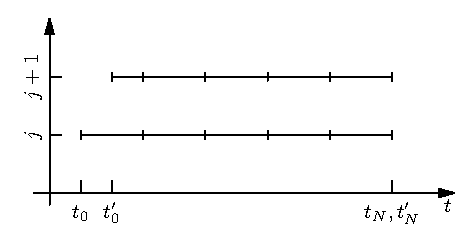
\includegraphics{mpc_subsampling.eps}}
        \subcaption{
            Reduction of the first sampling interval.
        }
        \label{fig.mpc_subsampling}
    \end{minipage}
    \hfill
    \begin{minipage}[t]{0.49\textwidth}
        \centering{%
        \includegraphics{mpc_nosubsampling.eps}}
        \subcaption{
            Shift of the whole preview horizon.
        }
        \label{fig.mpc_nosubsampling}
    \end{minipage}
    \caption[Sampling of the preview horizon.]{
        Sampling of the preview horizon on iterations $j$ and $j+1$
        with $T_c = T/2$ and $t_0^{\prime} = t_0 + T_c$.
    }
    \label{fig.mpc_sampling}
\end{figure}


The desired frequency of whole body motion control is higher than
$200~[\MT{Hz}]$, which corresponds to duration of a control interval $T_c$ in
the order of milliseconds \cite{Kuindersma2014icra, Herzog2015auro,
Saab2013tro}. Therefore, if an \ac{MPC} problem is resolved at such frequency,
in the form of \ac{MMPC} or as a part of two-stage control, it is necessary to
address discrepancy between $T$ and $T_c$. In this work we tried to employ two
heuristics for this purpose:
%
\begin{itemize}
    \item Reducing the first sampling interval $T_0$ by $T_c$ on each control
        iteration (\cref{fig.mpc_subsampling}). This can be interpreted as
        gradual removal of implicit \tn{move blocking} constraints, which
        impose that the control input is constant during $T_0$ (see also
        \cite{Cagienard2007jpc}).

    \item Shifting the whole preview horizon by $T_c$ on each control iteration
        (\cref{fig.mpc_nosubsampling}). The time instants at which constraints
        are imposed are shifted too. Thus, there is a problem of
        synchronization of changes in the model with the boundaries of sampling
        intervals as suggested in \cref{sec.discret_variation}. For example,
        consider a situation when a switch from a double to a single support is
        scheduled at time $t_0 + T$. If the constraint on the \ac{CoP} position
        is shifted from $t_0 + T$ with the preview horizon, there is a risk
        that the anticipated motion does not comply with this constraint at the
        instant of the switch. If we preserve constraints at such instants, the
        underlying optimization problem often becomes infeasible since the
        considered heuristic impairs recursive feasibility even in the case of
        time-invariant systems.
\end{itemize}
%
In either case, the structure of the \ac{MPC} problem changes significantly
from one control iteration to another due to changes in constraints. As a
result, the solutions obtained on subsequent iterations in general are not
equal on interval $[t_0^{\prime}, t_N]$, even in an ideal situation. In our
experience, this results in variations with period $T$ in solutions. Similar
behavior observed in \cite{Henze2014iros} is presumably caused by the same
reason. The second heuristic, however, yields much better results, which are
demonstrated later in \cref{ch.simulations}.


In conclusion of this discussion, it is necessary to emphasize that further
investigation of the sampling issue is needed, since neither of the proposed
heuristics is completely satisfactory.



%%%%%%%%%%%%%%%%%%%%%%%%%%%%%%%%%%%%%%%%%%%%%%%%%%%%%%%%%%%%%%%%%%%%%%%%%%%%%%%%
%%%%%%%%%%%%%%%%%%%%%%%%%%%%%%%%%%%%%%%%%%%%%%%%%%%%%%%%%%%%%%%%%%%%%%%%%%%%%%%%
%%%%%%%%%%%%%%%%%%%%%%%%%%%%%%%%%%%%%%%%%%%%%%%%%%%%%%%%%%%%%%%%%%%%%%%%%%%%%%%%
\section{Conclusion}

This chapter develops on the ideas and results of
\cref{ch.balance,ch.modeling}. We introduce \acf{MPC} as the tool for motion
anticipation and discretize approximate models constructed in
\cref{ch.modeling}, so that they can be used in \ac{MPC}. Then we construct
capturability constraints for these models to enforce capturability of
anticipated motion as suggested in \cref{ch.balance}. In addition to this, we
present our \acf{MMPC} approach to whole body motion control and anticipation
\cite{Sherikov2014humanoids, Sherikov2015humanoids}, and discuss some technical
details of \ac{MPC} implementation.

%-------------------------------------------------------------------------------
\chapter{Prioritized Linear Least-Squares Optimization}
\label{ch.optimization}
\acresetall
%-------------------------------------------------------------------------------

Whole-body motion control and motion anticipation problems considered in
\cref{ch.modeling,ch.mpc} fall within the framework of \ac{PLLS} optimization,
which is the topic of the present chapter. We briefly outline the general
concepts behind \ac{PLLS} optimization in
\cref{sec.least_square_intro,sec.prioritization} without going into details of
the algorithms for solution of \ac{PLLS} problems. In the following
\cref{sec.pllso_examples} we present a number of examples of \ac{PLLS} problems
used in our works. \cref{sec.hierarchy_efficiency} lists a few general
techniques, which allow for increasing the computational performance of the
\ac{PLLS} solvers.



%%%%%%%%%%%%%%%%%%%%%%%%%%%%%%%%%%%%%%%%%%%%%%%%%%%%%%%%%%%%%%%%%%%%%%%%%%%%%%%%
%%%%%%%%%%%%%%%%%%%%%%%%%%%%%%%%%%%%%%%%%%%%%%%%%%%%%%%%%%%%%%%%%%%%%%%%%%%%%%%%
%%%%%%%%%%%%%%%%%%%%%%%%%%%%%%%%%%%%%%%%%%%%%%%%%%%%%%%%%%%%%%%%%%%%%%%%%%%%%%%%
\section{Introduction to Linear Least Squares Optimization}\label{sec.least_square_intro}

The basic building block of the \ac{PLLS} framework is a system of linear
inequalities
%
\begin{equation}\label{eq.basic_ls_ineq}
    \ubarV{\objb}
    \le
    \objA \x
    \le
    \barV{\objb}
    ,
\end{equation}
%
where $\x$ is the vector of decision variables, $\objA$ is some matrix,
$\ubarV{\objb}$ and $\barV{\objb}$ are vectors of lower and upper bounds. This
system is satisfied in the least-squares sense, and, hence, can be posed as a
\ac{QP}
%
\begin{equation}\label{eq.basic_ls_opt}
    \begin{aligned}
        \MINIMIZE{\x, \violation} & \NORME{\violation}^2 \\
        \SUBJECTTO              & \ubarV{\objb} \le \objA \x  -  \violation \le \barV{\objb},
    \end{aligned}
\end{equation}
%
where vector $\violation$ contains \tn{violations} of the respective inequalities
\cite{Bramley1994jsc, Escande2014ijrr}. A solution $(\x^\star, \violation^\star)$ of
\eqref{eq.basic_ls_opt} always exists, but may be nonunique.


In the rest of the thesis we call a system of inequalities in the form
\cref{eq.basic_ls_ineq} an \tn{objective}, individual inequality in an
objective is called a \tn{constraint}. For convenience, constraints in an
objective are subdivided into groups called \tn{tasks}, since they often
correspond to tasks of the whole body motion control introduced in
\cref{sec.wbm_control}. We presume that all objectives are satisfied in the
least-squares sense, therefore, vectors of violations $\violation$ are usually
omitted for simplicity. We also presume, that systems of constraints are solved
using an \tn{active set} strategy \cite[Chapter~16]{Nocedal2006numopt}. Many
presentational choices of this chapter are dictated by the intrinsic properties
of active set strategies, whose key idea is iterative \tn{activation} and
\tn{deactivation} of inequality constraints in the search for a solution. A
constraint is called \tn{active} if it holds as an equality, \IE, equality
constraints with $\ubarV{\objb} = \barV{\objb}$ are always active, inequality
constraints are active when their bounds are reached or violated.



%%%%%%%%%%%%%%%%%%%%%%%%%%%%%%%%%%%%%%%%%%%%%%%%%%%%%%%%%%%%%%%%%%%%%%%%%%%%%%%%
%%%%%%%%%%%%%%%%%%%%%%%%%%%%%%%%%%%%%%%%%%%%%%%%%%%%%%%%%%%%%%%%%%%%%%%%%%%%%%%%
%%%%%%%%%%%%%%%%%%%%%%%%%%%%%%%%%%%%%%%%%%%%%%%%%%%%%%%%%%%%%%%%%%%%%%%%%%%%%%%%
\section{Prioritization of objectives}\label{sec.prioritization}

Let us consider an equality objective composed of two tasks
%
\begin{equation}\label{eq.two_tasks_weighted}
    \begin{bmatrix}
        \gamma_1 \objA_1 \\
        \gamma_2 \objA_2 \\
    \end{bmatrix}
    \x
    =
    \begin{bmatrix}
        \gamma_1 \V{\objb}_1 \\
        \gamma_2 \V{\objb}_2 \\
    \end{bmatrix}
    ,
\end{equation}
%
where $\gamma_1$ and $\gamma_2$ are positive scalars. This objective
corresponds to the multicriterion optimization problem
\cite[Chapter~4]{Boyd2004conopt}
%
\begin{equation}
    \begin{aligned}
        \MINIMIZE{\x}    &   \gamma_1^2 \NORME{\objA_1 \x - \V{\objb}_1}^2 + \gamma_2^2 \NORME{\objA_2 \x - \V{\objb}_2}^2. \\
    \end{aligned}
\end{equation}
%
Tasks are said to be compatible, if they are violated to the same extent when
combined into an objective and when satisfied independently from each other.
Weights $\gamma_1$ and $\gamma_2$ determine a trade-off between incompatible
tasks, and have no effect otherwise.


In many practical situations trade-offs between tasks are unacceptable, since
some of the tasks have \tn{strictly} (or \tn{infinitely}) higher priority than
others. The classic example of such strict prioritization is \tn{The Three Laws
of Robotics} introduced by Isaac Asimov in his science-fiction works
\cite{ThreeLaws}:
%
\begin{hierarchy}
    \level \tn{A robot may not injure a human being or, through inaction, allow
    a human being to come to harm.}

    \level \tn{A robot must obey the orders given it by human beings, except
    where such orders would conflict with the First Law.}

    \level \tn{A robot must protect its own existence as long as such
    protection does not conflict with the First or Second Laws.}
\end{hierarchy}
%
A set of tasks organized in accordance with their priorities is called a
\tn{hierarchy} or \tn{stack of tasks} \cite{Mansard2009tro}.


Let us assign strictly higher priority to the first task in
\cref{eq.two_tasks_weighted} to obtain the hierarchy composed of two objectives
%
\begin{hierarchy}[hr.two_tasks_prioritized]
    \level $\objA_1 \x = \V{\objb}_1$
    \level $\objA_2 \x = \V{\objb}_2$
\end{hierarchy}
%
where weights $\gamma_1$ and $\gamma_2$ are meaningless and therefore omitted.
Hierarchies of such form were originally introduced in the field of robotics to
exploit \tn{redundancy} of manipulators with respect to the primary objective
\cite{Liegeois1977tsmc}. The secondary objective is then used to express
preferences in the way of execution of the primary objective, which can be
realized nonuniquely. Prioritization prevents degradation of performance of the
primary objective due to secondary objectives.



%%%%%%%%%%%%%%%%%%%%%%%%%%%%%%%%%%%%%%%%%%%%%%%%%%%%%%%%%%%%%%%%%%%%%%%%%%%%%%%%
\subsection{Solving a hierarchy}

The classic way to obtain the solution of \cref{hr.two_tasks_prioritized} is to
perform null space projections using a generalized pseudoinverse $(\cdot)^{\#}$
\cite{Siciliano1991icar}:
%
\begin{equation}
    \x^{\star}
    =
    \objA_1^{\#}
    \V{\objb}_1
    +
    \left(
        \objA_2
        (
            \M{I}
            -
            \objA_1^{\#}
            \objA_1
        )
    \right)^{\#}
    (
        \V{\objb}_2
        -
        \objA_2
        \objA_1^{\#}
        \V{\objb}_1
    )
\end{equation}
%
An arbitrary number of priority levels can be handled with iterative projections.


Projections have a number of disadvantages, in particular, they do not account
for inequalities. This drawback was addressed in \cite{Kanoun2011tro} using
cascades of \ac{QP}'s. For example, a hierarchy of two inequality objectives
%
\begin{hierarchy}[hr.two_inequality_objectives]
    \level $\ubarV{\objb}_1 \le \objA_1 \x \le \barV{\objb}_1$
    \level $\ubarV{\objb}_2 \le \objA_2 \x \le \barV{\objb}_2$
\end{hierarchy}
%
can be solved with two \ac{QP}'s:
%
\begin{enumerate}
    \item First, we find minimal violation of the first objective
        $\violation_1^{\star}$ using
        %
        \begin{equation}
            \begin{aligned}
                \MINIMIZE{\x,\violation_1}  & \NORME{\violation_1}^2 \\
                \SUBJECTTO                  & \ubarV{\objb}_1 \le \objA_1 \x - \violation_1 \le \barV{\objb}_1.
            \end{aligned}
        \end{equation}
        %

    \item Then the optimal violation of the second objective is determined with
        %
        \begin{equation}
            \begin{aligned}
                \MINIMIZE{\x,\violation_2}  & \NORME{\violation_2}^2 \\
                \SUBJECTTO                  & \ubarV{\objb}_1 \le \objA_1 \x - \violation_1^{\star} \le \barV{\objb}_1\\
                                            & \ubarV{\objb}_2 \le \objA_2 \x - \violation_2 \le \barV{\objb}_2.
            \end{aligned}
        \end{equation}
        %
\end{enumerate}
%
A similar approach was proposed in the field of \ac{MPC} to cope with
infeasibilities of constraints \cite{Vada1999ifac}.


Recent developments in numerical methods, however, allow for solution of
hierarchies with equalities and inequalities in much more efficient way than
null space projections and cascades of \ac{QP}'s \cite{Escande2014ijrr,
Dimitrov2015preprint}. Efficiency is achieved using dedicated active set
strategies, one of which was implemented in our research group in the software
package \sn{LexLS} \cite{Dimitrov2015preprint}. \sn{LexLS} is the primary
optimization tool employed in this thesis.



%%%%%%%%%%%%%%%%%%%%%%%%%%%%%%%%%%%%%%%%%%%%%%%%%%%%%%%%%%%%%%%%%%%%%%%%%%%%%%%%
\subsection{Singularities and regularization}\label{sec.regularization}

It is recognized that solvers for hierarchies may experience numerical
difficulties near singularities \cite{Siciliano1991icar, Deo1995jirs,
Kanoun2011tro}. In robotic applications this leads to control inputs taking
unacceptably high values, if unconstrained, or flipping between the bounds at
high frequency otherwise.



One way to cope with deteriorated behavior near singularities is to introduce
regularization. Standard \tn{Tikhonov regularization} is implemented by
extending the $\ell$-th objective as follows
%
\begin{equation}\label{eq.tikhonov_regularization}
    \begin{bmatrix}
        \ubarV{\objb}_{\ell} \\
        \V{0} \\
    \end{bmatrix}
    \le
    \begin{bmatrix}
        \objA_{\ell} \\
        \gamma_{r,\ell} \V{I} \\
    \end{bmatrix}
    \x
    \le
    \begin{bmatrix}
        \barV{\objb}_{\ell} \\
        \V{0} \\
    \end{bmatrix}
    ,
\end{equation}
%
where $\gamma_{r,\ell} \in \RR_{\ge 0}$ is a \tn{damping factor}, which is used
to trade-off accuracy of the solution with the norm of $\x^{\star}$. The best
results are achieved, when the value of $\gamma_{r,\ell}$ is chosen
automatically and is fading to zero far from singularities. The objective
\cref{eq.tikhonov_regularization} corresponds to the \ac{QP}
%
\begin{equation}
    \begin{aligned}
        \MINIMIZE{\x, \violation_{\ell}} & \NORME{\violation_{\ell}}^2 + \gamma_{r,\ell}^2 \NORME{\x}^2\\
        \SUBJECTTO                  & \ubarV{\objb}_j \le \objA_j \x  -  \violation_j^{\star} \le \barV{\objb}_j,   && j \in \{1, ..., \ell-1\}, \\
                                    & \ubarV{\objb}_{\ell} \le \objA_{\ell} \x  -  \violation_{\ell} \le \barV{\objb}_{\ell}.
    \end{aligned}
\end{equation}
%
Note that this optimization problem has a unique solution $\x$. When a cascade
of \ac{QP}'s is used to solve the hierarchy, this means that the regularizing
task $\gamma_{r,\ell} \V{I} \x = \V{0}$ must be omitted in $\ell+1$ \ac{QP} in
order to be able to execute objectives of lower importance
\cite[Chapter~3]{Kanoun2009thesis}
%
\begin{equation}
    \begin{aligned}
        \MINIMIZE{\x, \violation_{\ell+1}} & \NORME{\violation_{\ell+1}}^2\\
        \SUBJECTTO                      & \ubarV{\objb}_j \le \objA_j \x  -  \violation_j^{\star} \le \barV{\objb}_j,  && j \in \{1, ..., \ell\}, \\
                                        & \ubarV{\objb}_{\ell+1} \le \objA_{\ell+1} \x  -  \violation_{\ell+1} \le \barV{\objb}_{\ell+1}.
    \end{aligned}
\end{equation}
%
Similarly, dedicated solvers like those proposed in \cite{Escande2014ijrr,
Dimitrov2015preprint} should implement special logic to handle regularization
tasks.


We believe that Tikhonov regularization is not the best choice in general. For
example, if $\objA_{\ell} = \M{I}$ it is more reasonable to bias $\x$ towards
$\V{\objb}_{r,\ell} = \ubarV{\objb}_{\ell} + (\barV{\objb}_{\ell} -
\ubarV{\objb}_{\ell}) / 2$ rather than $\V{0}$. Hence, we advocate for
regularization using a general matrix $\objA_{r,\ell}$ and vector
$\V{\objb}_{r,\ell}$ \cite{Sherikov2015humanoids}
%
\begin{equation}
    \begin{bmatrix}
        \ubarV{\objb}_{\ell} \\
        \gamma_{r,\ell} \V{\objb}_{r,\ell} \\
    \end{bmatrix}
    \le
    \begin{bmatrix}
        \objA_{\ell} \\
        \gamma_{r,\ell} \objA_{r,\ell} \\
    \end{bmatrix}
    \x
    \le
    \begin{bmatrix}
        \barV{\objb}_{\ell} \\
        \gamma_{r,\ell} \V{\objb}_{r,\ell} \\
    \end{bmatrix}
    ,
\end{equation}
%
which corresponds to the least-squares problem
%
\begin{equation}
    \begin{aligned}
        \MINIMIZE{\x, \violation_{\ell}} & \NORME{\violation_{\ell}}^2 + \gamma_{r,\ell}^2 \NORME{\objA_{r,\ell} \x - \V{\objb}_{r,\ell}}^2\\
        \SUBJECTTO                  & \ubarV{\objb}_j \le \objA_j \x  -  \violation_j^{\star} \le \barV{\objb}_j,  && j \in \{1, ..., \ell-1\}, \\
                                    & \ubarV{\objb}_{\ell} \le \objA_{\ell} \x  -  \violation_{\ell} \le \barV{\objb}_{\ell}.
    \end{aligned}
\end{equation}
%
Regularization can be tuned by changing the damping factor $\gamma_{r,\ell}$.
The choice of $\objA_{r,\ell}$ and $\V{\objb}_{r,\ell}$ may appear to be
nontrivial, but in most practical applications these terms are already defined
and imposed on the very last level of the hierarchy to resolve any remaining
redundancy. Our practical experience also suggests, that regularization with
the last objective of a hierarchy is much easier to tune than Tikhonov
regularization.



%%%%%%%%%%%%%%%%%%%%%%%%%%%%%%%%%%%%%%%%%%%%%%%%%%%%%%%%%%%%%%%%%%%%%%%%%%%%%%%%
%%%%%%%%%%%%%%%%%%%%%%%%%%%%%%%%%%%%%%%%%%%%%%%%%%%%%%%%%%%%%%%%%%%%%%%%%%%%%%%%
%%%%%%%%%%%%%%%%%%%%%%%%%%%%%%%%%%%%%%%%%%%%%%%%%%%%%%%%%%%%%%%%%%%%%%%%%%%%%%%%
\section{Examples and applications}\label{sec.pllso_examples}

A hierarchy of objectives is not a new concept, but it has experienced a
significant growth of interest in the recent years due to its spreading in the
control of humanoid robots \cite{Kanoun2009thesis, Saab2013tro,
Sentis2007thesis}. We believe that the reason for this is not only the power of
prioritization, but also the clearness and conciseness of representation of
robot control problems in the form of a hierarchy \cite{Dimitrov2014jrs}. The
second reason, however, led to what we believe to be a misuse of hierarchies
and to a certain disappointment in them.


We would like to stress that posing optimization problems as hierarchies is not
always meaningful, but should be considered for the following purposes
%
\begin{itemize}
    \item Relaxation of objectives and resolution of conflicts between them by
        introducing strict priorities. Note that in the literature it is common
        to prioritize objectives even if they are compatible
        \cite[Chapter~5]{Sentis2007thesis}, \cite{Dietrich2015ijrr,
        Saab2013tro}. Consequently, many proposed hierarchies can be
        reformulated as \ac{QP}'s and solved with off-the-shelf software
        without qualitative changes in the robot behavior.

    \item Increase of the computational performance due to variable
        eliminations. Prioritization of the objectives is equivalent to
        variable eliminations, which are commonly performed in robot control as
        preliminary steps \cite{Dimitrov2014jrs}, and, likewise, allows for
        faster solution of optimization problems \cite{Dimitrov2015preprint}.
        This point is explained in more detail using an example in
        \cref{sec.variable_elimination}.
\end{itemize}
%
In this section we brought together several examples to illustrate situations
where hierarchies are useful. The ideas behind these examples are general and
are not limited to humanoid robot control.



%%%%%%%%%%%%%%%%%%%%%%%%%%%%%%%%%%%%%%%%%%%%%%%%%%%%%%%%%%%%%%%%%%%%%%%%%%%%%%%%
\subsection{Variable elimination}\label{sec.variable_elimination}

Variable elimination, which is ubiquitously performed in robotics, can be
perceived as prioritization of constraints. We illustrate this with a simple
hierarchy corresponding to an \ac{MPC} problem
%
\begin{hierarchy}[hr.mpc_simple]
    \level  $\V{x}_{k+1} = \M{A}_k \V{x}_k + \M{B}_k \V{u}_k$\\
            $\V{x}_{k+1} \in \SET{X}_{k+1}$\\
            $\V{u}_k \in \SET{U}_k$\\
            $\V{x}_N \in \SET{T}$

    \level  $\M{\Gamma}_{\V{x}} \V{x}_{k+1} = \V{0}$\\
            $\M{\Gamma}_{\V{u}} \V{u}_k = \V{0}$

    \vars{$\x = (\V{x}_{k+1}, \V{u}_k)$ with $k \in \{0, ..., N-1\}$}
\end{hierarchy}
%
where $\V{x}_N \in \SET{T}$ is a terminal or capturability constraint,
$\M{\Gamma}_{\V{x}}$ and $\M{\Gamma}_{\V{u}}$ are some weighting matrices.


In practice it is common to perform so called \tn{condensing} of the considered
\ac{MPC} problem \cite{Bock1984ifac}, \cref{app.condensing}. The idea of
condensing consists in
%
\begin{itemize}
    \item expressing states $(\V{x}_1, ..., \V{x}_N)$ through the current state
        $\V{x}_0$ and control inputs $(\V{u}_0, ..., \V{u}_{N-1})$ using the
        equation of dynamics of the system and

    \item elimination of $(\V{x}_1, ..., \V{x}_N)$ from the problem.
\end{itemize}
%
This procedure can be interpreted as satisfying the dynamics first and the
remaining objectives later and, thus, can be posed as the hierarchy
%
\begin{hierarchy}[hr.dynamics_elimination]
    \level  $\V{x}_{k+1} = \M{A}_k \V{x}_k + \M{B}_k \V{u}_k$

    \level  $\V{x}_{k+1} \in \SET{X}_{k+1}$\\
            $\V{u}_k \in \SET{U}_k$\\
            $\V{x}_N \in \SET{T}$

    \level  $\M{\Gamma}_{\V{x}} \V{x}_{k+1} = \V{0}$\\
            $\M{\Gamma}_{\V{u}} \V{u}_k = \V{0}$

    \vars{$\x = (\V{x}_{k+1}, \V{u}_k)$ with $k \in \{0, ..., N-1\}$}
\end{hierarchy}
%
The null space of the objective \cref{hr.dynamics_elimination.1}, where
objectives \cref{hr.dynamics_elimination.2} and
\cref{hr.dynamics_elimination.3} are satisfied, is of lower dimension than the
space of all vectors $\x$ \cite{Kanoun2011tro, deLasa2010trangraph,
Dimitrov2015preprint}. A \ac{PLLS} solver can exploit this fact to
automatically eliminate variables and avoid unnecessary computations
\cite{Dimitrov2015preprint}.


Representation of variable eliminations with hierarchies is appealing, since it
emphasizes the essence of the problem rather than implementation details.
Therefore, it encourages development of general approaches to solving
hierarchies instead of \tn{ad-hoc} methods for solving particular optimization
and control problems. Note that generality does not imply lower performance,
since the solvers can take advantage of the structure of the problem as it is
done during manual elimination of variables (see
\cref{sec.hierarchy_efficiency}).


The above conclusion is not limited to condensing in \ac{MPC} and applies to
many problems in robotics, for example, elimination of the external forces in
whole body motion controllers \cite[Chapter~2]{Sentis2007thesis}
\cite{Mansard2012icra}, or elimination of joint torques \cite{Herzog2015auro}.



%%%%%%%%%%%%%%%%%%%%%%%%%%%%%%%%%%%%%%%%%%%%%%%%%%%%%%%%%%%%%%%%%%%%%%%%%%%%%%%%
\subsection{Relaxation of capturability and terminal constraints}

Consider \cref{hr.mpc_simple} corresponding to a general \ac{MPC} problem. It
is recognized that the terminal (or capturability) constraint in it may be the
source of infeasibility \cite[Chapter~8]{Rossiter2003mpc}. If, for various
reasons, neither the length of the preview horizon nor the terminal set
$\SET{T}$ can be adjusted to avoid infeasibility, a reasonable option is
relaxation. In this case we have to take into account two goals: ({\bf i})
relaxation of the terminal constraint should not interfere with other high
priority tasks, ({\bf ii}) low priority objectives should not interfere with
satisfaction of the terminal constraint. We achieve both goals by adding a
separate priority level for the terminal or capturability constraint
\cite{Sherikov2014humanoids}
%
\begin{hierarchy}[hr.mpc_with_capturability]
    \level  $\V{x}_{k+1} = \M{A}_k \V{x}_k + \M{B}_k \V{u}_k$\\
            $\V{x}_{k+1} \in \SET{X}_{k+1}$\\
            $\V{u}_k \in \SET{U}_k$

    \level  $\V{x}_N \in \SET{T}$

    \level  $\M{\Gamma}_{\V{x}} \V{x}_{k+1} = \V{0}$\\
            $\M{\Gamma}_{\V{u}} \V{u}_k = \V{0}$

    \vars{$\x = (\V{x}_{k+1}, \V{u}_k)$ with $k \in \{0, ..., N-1\}$}
\end{hierarchy}
%



%%%%%%%%%%%%%%%%%%%%%%%%%%%%%%%%%%%%%%%%%%%%%%%%%%%%%%%%%%%%%%%%%%%%%%%%%%%%%%%%
\subsection{Time optimal Model Predictive Control}\label{sec.time_optimal_mpc}

In some situations, hierarchies can be used for expressing backup control
goals, for example, hierarchy
%
\begin{hierarchy}
    \level $\ubarV{\objb} \le \x \le \barV{\objb}$
    \levelLabel{$\dots$} $\dots$
    \levelLabel{$\V{\ell}$:} $\displaystyle \x = \ubarV{\objb} + \frac{1}{2} \left( \barV{\objb} - \ubarV{\objb} \right)$
\end{hierarchy}
%
can be interpreted as follows: if satisfaction of the equality task on $\x$ on
level $\ell$ is impossible, fall back to bounding of $\x$. We combined this
idea with the idea of hierarchical relaxation of the terminal constraint to
obtain a time optimal \ac{MPC} scheme hinted in
\cite[Chapter~8]{Kerrigan2000thesis} and implemented in \cite{alHomsi2016icra}.
The goal of a time optimal controller is to reach the desired state
$\V{x}^{\DES}$ in minimal time. Hence, we can first try to achieve the goal
within the first sampling interval of the preview horizon, if not impossible --
within $2$ intervals, and so on until the end of preview horizon is reached. We
can formalize this process with a single hierarchy, where reaching
$\V{x}^{\DES}$ in $k+1$ sampling intervals in the preview horizon is infinitely
more important than reaching it in $k$ intervals:
%
\thesisHierarchyStyle{\setlength{\labelwidth}{1.5cm}\setlength{\leftmargin}{1.5cm}}
\begin{hierarchy}
    \level  $\V{x}_{k+1} = \M{A}_k \V{x}_k + \M{B}_k \V{u}_k$\\
            $\V{x}_{k+1} \in \SET{X}_{k+1}$\\
            $\V{u}_k \in \SET{U}_k$

    \level  $\V{x}_{N} = \V{x}^{\DES}$

    \levelLabel{$\dots$} $\dots$

    \levelLabel{$\V{N+1}$:}  $\V{x}_{1} = \V{x}^{\DES}$

    \levelLabel{$\V{N+2}$:}  $\M{\Gamma}_{\V{x}} \V{x}_{k+1} = \V{0}$\\
            $\M{\Gamma}_{\V{u}} \V{u}_k = \V{0}$

    \vars{$\x = (\V{x}_{k+1}, \V{u}_k)$ with $k \in \{0, ..., N-1\}$}
\end{hierarchy}
\thesisHierarchyStyle{}%
%
More information on implementation of this time optimal controller and results
of its evaluation can be found in \cite{alHomsi2016icra}.



%%%%%%%%%%%%%%%%%%%%%%%%%%%%%%%%%%%%%%%%%%%%%%%%%%%%%%%%%%%%%%%%%%%%%%%%%%%%%%%%
\subsection{Mixed Model Predictive Control}\label{sec.mmpc_hierarchy}

A sequence of actions can often be interpreted as a strict hierarchy between
them. We use this insight to present our \ac{MMPC} approach from a different
perspective.


The traditional approach to control of humanoid robots consists of two
sequential stages (see \cref{sec.mmpc})
%
\begin{enumerate}
    \item Anticipation, which can be performed using \ac{MPC} in the form of
        \cref{hr.mpc_with_capturability}. Assuming that the anticipation is
        performed at the same rate as whole body motion control, we extract the
        initial control $\V{u}_0^\star$ from the solution of the \ac{MPC} to
        feed it to the whole body motion controller.

    \item Execution of the desired values $\V{u}_0^\star$ obtained from the
        solution of \cref{hr.mpc_with_capturability} by a whole body motion
        controller. The controller is also based on a hierarchy, which
        incorporates the whole body \nameref{model.WB} model presented in
        \cref{sec.contact_constraints}:
        %
        \thesisHierarchyStyle{\setlength{\itemsep}{5pt}}
        \begin{hierarchy}[hr.wbc_controller]
            \level Dynamics of the robot
                    \begin{itemize}
                        \item $\displaystyle \M{H} \ddq + \V{h} = \Itorques\torques + m\T{\Jcom} \V{g} + \sum_{i=1}^M \T{\M{J}_i}
                            \begin{bmatrix}
                                \M{V}_i \V{\lambda}_i\\
                                \moment_i
                            \end{bmatrix}$
                    \end{itemize}
                   Fixed contact positions
                    \begin{itemize}
                        \item $\displaystyle \M{J}_i \ddq + \dotM{J}_i \dq = \V{0}$
                    \end{itemize}
                   Mechanical joint constraints
                    \begin{itemize}
                        \item $\displaystyle \ubar{\torques}  \le  \torques  \le  \bar{\torques}$
                        \item $\displaystyle \ubar{\ddq}^{\prime}  \le  \ddqn  \le  \bar{\ddq}^{\prime}$
                    \end{itemize}
                   Constraints on the contact wrenches
                    \begin{itemize}
                        \item $\displaystyle
                            \objA_{\moment,i}
                            \begin{bmatrix}
                                \V{\lambda}_i\\
                                \moment_i
                            \end{bmatrix}
                            \ge
                            \ubarV{\objb}_{\moment,i}
                            $
                        \item $\displaystyle \V{\lambda}_i \ge \V{0}$
                    \end{itemize}
                   A task with some $\objA_t$ and $\V{\objb}_t$ for tracking of the desired $\V{u}_0^\star$
                    \begin{itemize}
                        \item $\objA_t \begin{bmatrix} \x\\ \V{u}_0^\star \end{bmatrix} = \V{\objb}_t$
                    \end{itemize}

            \level Arbitrary whole body tasks (see \cref{sec.wbm_control}).

            \vars{$\x = (\ddq, \torques, \V{\lambda}_i, \moment_{i})$ with $i \in \{1, ..., M\}$}
        \end{hierarchy}
        \thesisHierarchyStyle{}%
        %
\end{enumerate}


After concatenation of \cref{hr.mpc_with_capturability,hr.wbc_controller} and
shuffling of the tasks in the resulting hierarchy we obtain an \ac{MMPC}
controller \cite{Sherikov2014humanoids, Sherikov2015humanoids}
%
\thesisHierarchyStyle{\setlength{\itemsep}{5pt}}
\begin{hierarchy}[hr.mmpc_general]
    \level Tasks of the whole body motion controller
            \begin{itemize}
                \item $\displaystyle \M{H} \ddq + \V{h} = \Itorques\torques + m\T{\Jcom} \V{g} + \sum_{i=1}^M \T{\M{J}_i}
                    \begin{bmatrix}
                        \M{V}_i \V{\lambda}_i\\
                        \moment_i
                    \end{bmatrix}$
                \item $\displaystyle \M{J}_i \ddq + \dotM{J}_i \dq = \V{0}$
                \item $\displaystyle \ubar{\torques}  \le  \torques  \le  \bar{\torques}$
                \item $\displaystyle \ubar{\ddq}^{\prime}  \le  \ddqn  \le  \bar{\ddq}^{\prime}$
                \item $\displaystyle
                    \objA_{\moment,i}
                    \begin{bmatrix}
                        \V{\lambda}_i\\
                        \moment_i
                    \end{bmatrix}
                    \ge
                    \ubarV{\objb}_{\moment,i}
                    $
                \item $\displaystyle \V{\lambda}_i \ge \V{0}$
            \end{itemize}
           Tasks of the \ac{MPC} controller
            \begin{itemize}
                \item $\V{x}_{k+1} = \M{A}_k \V{x}_k + \M{B}_k \V{u}_k$
                \item $\V{x}_{k+1} \in \SET{X}_{k+1}$
                \item $\V{u}_k \in \SET{U}_k$
            \end{itemize}
           The coupling task
            \begin{itemize}
                \item $\objA_t \x = \V{\objb}_t$
            \end{itemize}

    \level The capturability constraint
            \begin{itemize}
                \item $\V{x}_N \in \SET{T}$
            \end{itemize}

    \level Arbitrary whole body tasks\\
           Tasks of the \ac{MPC} controller
            \begin{itemize}
                \item $\M{\Gamma}_{\V{x}} \V{x}_{k+1} = \V{0}$
                \item $\M{\Gamma}_{\V{u}} \V{u}_k = \V{0}$
            \end{itemize}

        \vars{$\x = (\ddq, \torques, \V{\lambda}_i, \moment_{i}, \V{x}_{k+1}, \V{u}_k)$\\
        \makebox[3.3cm]{} with $i \in \{1, ..., M\}$ and $k \in \{0, ..., N-1\}$}
\end{hierarchy}
\thesisHierarchyStyle{}%
%
More detailed examples of this hierarchy are given in \cref{ch.simulations}.



%%%%%%%%%%%%%%%%%%%%%%%%%%%%%%%%%%%%%%%%%%%%%%%%%%%%%%%%%%%%%%%%%%%%%%%%%%%%%%%%
\subsection{Minimization of an optional contact force}

We extended \cref{hr.mmpc_general} in \cite{Sherikov2015humanoids} in such a
way, that the controller applies non-zero contact force at a certain contact
only when it is necessary to maintain balance or execute a whole body task.
This is achieved with a hierarchy, which can roughly be stated as
%
\begin{hierarchy}
    \level maintain balance
    \level execute whole body task
    \level minimize optional contact force
\end{hierarchy}
%
and is considered in detail in \cref{sec.optional_force}.



%%%%%%%%%%%%%%%%%%%%%%%%%%%%%%%%%%%%%%%%%%%%%%%%%%%%%%%%%%%%%%%%%%%%%%%%%%%%%%%%
%%%%%%%%%%%%%%%%%%%%%%%%%%%%%%%%%%%%%%%%%%%%%%%%%%%%%%%%%%%%%%%%%%%%%%%%%%%%%%%%
%%%%%%%%%%%%%%%%%%%%%%%%%%%%%%%%%%%%%%%%%%%%%%%%%%%%%%%%%%%%%%%%%%%%%%%%%%%%%%%%
\section{Solving hierarchies efficiently}\label{sec.hierarchy_efficiency}

Computational efficiency is one of the most important factors in real time
controllers. Hence, we aim at efficient resolution of hierarchies used in our
controllers. In order to achieve this, we employ a number of techniques, which
are reviewed in this section and are supported by \sn{LexLS} to various
degrees. The techniques are of general nature and are shared with conventional
active set \ac{QP} solvers, whose performance is studied extensively in the
literature \cite{Herceg2015ocam, Wang2010tcst, Ferreau2008ijrnc}.



%%%%%%%%%%%%%%%%%%%%%%%%%%%%%%%%%%%%%%%%%%%%%%%%%%%%%%%%%%%%%%%%%%%%%%%%%%%%%%%%
\subsection{Exploitation of the problem structure}\label{sec.problem_structure}

One of the ways to improve performance of the solver is to shape the
optimization problem in a beneficial manner and to inform the solver about the
structure of the problem.


%%%%%%%%%%%%%%%%%%%%%%%%%%%%%%%%%%%%%%%%%%%%%%%%%%%%%%%%%%%%%%%%%%%%%%%%%%%%%%%%
\subsubsection{Two-sided inequalities}

We formulate all objectives in such a way that they have both upper and lower
bounds:
%
\begin{equation}\label{eq.basic_ls_ineq2}
    \ubarV{\objb}
    \le
    \objA \x
    \le
    \barV{\objb}
    .
\end{equation}
%
The reason for this is that bounds $\ubarV{\objb} < \barV{\objb}$ cannot be
activated simultaneously, and an active set solver can exploit this fact to
reduce computational load. If one of the bounds is undefined it can be replaced
by some ``very large'' number. When $\ubarV{\objb} = \barV{\objb} = \V{\objb}$
the constraints are treated as equalities, which are always active.


%%%%%%%%%%%%%%%%%%%%%%%%%%%%%%%%%%%%%%%%%%%%%%%%%%%%%%%%%%%%%%%%%%%%%%%%%%%%%%%%
\subsubsection{Simple bounds}\label{sec.simple_bounds}

In some situations it is possible to express general inequalities
\cref{eq.basic_ls_ineq2} as \tn{simple bounds} or \tn{box constraints} on
the decision variables:
%
\begin{equation}\label{eq.simple_bounds}
    \ubarV{\objb}
    \le
    \x
    \le
    \barV{\objb}.
\end{equation}
%
Handling of such constraints can be implemented in a very efficient way
\cite{Gill1984tms, Ferreau2008ijrnc, Dimitrov2015preprint}. For this reason, we
reformulate \ac{MPC} problems to convert general inequalities to simple bounds,
\EG, \cite{Dimitrov2011icra}, \cref{sec.mpc_simple_bounds}.



%%%%%%%%%%%%%%%%%%%%%%%%%%%%%%%%%%%%%%%%%%%%%%%%%%%%%%%%%%%%%%%%%%%%%%%%%%%%%%%%
\subsubsection{Sparsity}\label{sec.sparsity}

We call a task \tn{sparse} if the corresponding matrix $\objA$ contains a large
number of zeros. A task with simple bounds \cref{eq.simple_bounds} is a typical
example of a sparse task. Other examples are the tasks on the first level of
\cref{hr.mpc_simple} corresponding to \ac{MPC} constraints. This type of
sparsity is sometimes exploited in \ac{QP} solvers designed for \ac{MPC}
problems \cite{Wang2010tcst, Dimitrov2011iros}. \sn{LexLS} currently can take
advantage of the sparsity only in the case of simple bounds on the first level
of a hierarchy.



%%%%%%%%%%%%%%%%%%%%%%%%%%%%%%%%%%%%%%%%%%%%%%%%%%%%%%%%%%%%%%%%%%%%%%%%%%%%%%%%

\subsection{Early termination}\label{sec.early_termination}

Control problems are typically resolved with a constant rate, which means that
there is an upper limit on the time available for computations. Hence, the
solvers should provide a mechanism for early termination in order to fit within
the limits \cite{Ferreau2008ijrnc, Wang2010tcst}. Termination can be triggered
by a timer or the number of iterations of the solver. One iteration of an
active set solver typically corresponds to activation or deactivation of a
single constraint.


Early termination is potentially dangerous since the solution returned by the
solver is suboptimal. In the \ac{PLLS} framework it implies that violations of
objectives can be unacceptably large, \IE, high priority constraints may not be
satisfied even if they are feasible. This is not an issue, if a solver is
provided with an initial guess of the solution, which is feasible with respect
to the primary tasks, and the solver does not increase violations of the
objectives while searching for the solution.



%%%%%%%%%%%%%%%%%%%%%%%%%%%%%%%%%%%%%%%%%%%%%%%%%%%%%%%%%%%%%%%%%%%%%%%%%%%%%%%%
\subsection{Warm start}

Since the hierarchies for control of robots are resolved at high frequency, the
solutions usually do not change much from one control iteration to another
\cite{Kuindersma2014icra, Escande2014ijrr, Sherikov2014humanoids}. This allows
to use the solution $\x^\star$ and the active set obtained at $i$-th iteration
to warm start the solver on $i+1$ iteration.


%%%%%%%%%%%%%%%%%%%%%%%%%%%%%%%%%%%%%%%%%%%%%%%%%%%%%%%%%%%%%%%%%%%%%%%%%%%%%%%%
\subsubsection{Guessing the solution}

Ideally, a solution guess should be feasible with respect to the high priority
objectives, in this case it is safe to terminate the solver before the solution
is found. However, determination of such a guess for hierarchies employed in
this thesis is not trivial, and we simply reuse the solution $\x^\star$ from
the previous control iteration. When the dimension of $\x$ changes, for
example, due to a switch from a single to a double support, it is necessary to
drop parts of the previous solution or provide a guess for the missing parts of
$\x$. Our main heuristic for assigning the missing parts is to avoid activation
of the corresponding inequality constraints.


An alternative approach to generate a guess is to solve an auxiliary hierarchy,
which has roughly the following structure
%
\begin{hierarchy}
    \level Important equality tasks.

    \level Important inequality tasks $\ubarV{\objb} \le \objA \x \le
        \barV{\objb}$ converted to equalities\\
        $\displaystyle \objA \x = \ubarV{\objb} + \frac{1}{2} \left(\barV{\objb} - \ubarV{\objb} \right)$\\
        and weighted with respect to each other.
\end{hierarchy}
%
and guarantees satisfaction of primary equality constraints if the solver is
terminated prematurely. Solution of this hierarchy may result in a better
guess, but it is time consuming and the weights have to be tuned carefully
depending on the setting.



%%%%%%%%%%%%%%%%%%%%%%%%%%%%%%%%%%%%%%%%%%%%%%%%%%%%%%%%%%%%%%%%%%%%%%%%%%%%%%%%
\subsubsection{Guessing the active set}

In addition to the solution guess we provide the solver with a guess of the
active set, \IE, the set of active inequality constraints at the solution
\cite{Ferreau2008ijrnc, Escande2014ijrr, Kuindersma2014icra}. Since the number
of constraints also changes from one control iteration to another, we employ a
number of task specific heuristics for modifying the active set when such
changes occur.



%%%%%%%%%%%%%%%%%%%%%%%%%%%%%%%%%%%%%%%%%%%%%%%%%%%%%%%%%%%%%%%%%%%%%%%%%%%%%%%%
\subsection{Preprocessing}\label{sec.plls_preprocessing}

Since \sn{LexLS} has rather limited capabilities for exploiting the problem
structure (see \cref{sec.problem_structure}), we perform several preprocessing
steps to improve performance.



%%%%%%%%%%%%%%%%%%%%%%%%%%%%%%%%%%%%%%%%%%%%%%%%%%%%%%%%%%%%%%%%%%%%%%%%%%%%%%%%
\subsubsection{Variable elimination}

During the preprocessing, we eliminate some of the variables in the hierarchies
to reduce computational load. In particular, we eliminate the whole body joint
torques $\torques$ as described in \cref{sec.momenta_based_nonlinear} and
perform condensing of \ac{MPC} problems \cite{Bock1984ifac},
\cref{app.condensing}.



%%%%%%%%%%%%%%%%%%%%%%%%%%%%%%%%%%%%%%%%%%%%%%%%%%%%%%%%%%%%%%%%%%%%%%%%%%%%%%%%
\subsubsection{Removing excessive simple bounds}

Simple bounds on the joint accelerations $\ddqn$ are overdetermined as
explained in \cref{app.jointconstraints}. Due to simplicity of these
constraints, it is possible to reduce their number using a trivial procedure.



%%%%%%%%%%%%%%%%%%%%%%%%%%%%%%%%%%%%%%%%%%%%%%%%%%%%%%%%%%%%%%%%%%%%%%%%%%%%%%%%
\subsubsection{Removing excessive equality constraints}

In some cases the matrix $\objA$ in an equality task $\objA \x = \V{\objb}$
includes linearly dependent constraints. If this task does not change on each
control iteration, it is beneficial to remove excessive constraints using a
\tn{QR-decomposition} of $\objA$ with column pivoting
\cite[Chapter~5]{Golub1996matrix}.



%%%%%%%%%%%%%%%%%%%%%%%%%%%%%%%%%%%%%%%%%%%%%%%%%%%%%%%%%%%%%%%%%%%%%%%%%%%%%%%%
%%%%%%%%%%%%%%%%%%%%%%%%%%%%%%%%%%%%%%%%%%%%%%%%%%%%%%%%%%%%%%%%%%%%%%%%%%%%%%%%
%%%%%%%%%%%%%%%%%%%%%%%%%%%%%%%%%%%%%%%%%%%%%%%%%%%%%%%%%%%%%%%%%%%%%%%%%%%%%%%%
\section{Conclusion}

We introduced the \acf{PLLS} framework and illustrated it with several
optimization problems proposed in our works \cite{Sherikov2014humanoids,
Sherikov2014humanoids, alHomsi2016icra}. In particular, we presented an
interpretation of \acf{MMPC} problem as a result of merging and
reprioritization of motion anticipation and whole body motion controllers. In
addition to that we outlined several techniques, which we employ to reduce
computational load when solving \ac{PLLS} problems.

%-------------------------------------------------------------------------------
\chapter{Simulations and experiments}
\label{ch.simulations}
\acresetall
%-------------------------------------------------------------------------------

In the present chapter we compile and extend simulation results presented in
\cite{Sherikov2014humanoids, Sherikov2015humanoids} and overview results
obtained in \cite{Brasseur2015humanoids, Agravante2016preprint,
alHomsi2016icra}. \cref{sec.task_walk} is based on \cite{Sherikov2014humanoids}
and is focused on the interplay between whole body tasks and walking motions in
a \ac{MMPC} problem. The next \cref{sec.optional_force} describes a more
sophisticated \ac{MMPC} controller, where we introduce prioritization in
contact force distribution. Both sections highlight the importance of the
capturability constraints for balance preservation. The final
\cref{sec.collaboration_results} discusses results of the collaborative works
\cite{Brasseur2015humanoids, Agravante2016preprint, alHomsi2016icra}. Videos
illustrating the presented works can be found on the web page of the author
\cite{SHERIKOVsite}.


Controllers considered in \cref{sec.task_walk,sec.optional_force} are
formulated as \ac{PLLS} problems, which are solved using a dedicated solver --
\sn{LexLS} \cite{Dimitrov2015preprint}. \sn{LexLS} is implemented in \sn{C++}
using the \sn{Eigen} template library \cite{EIGENsite}. The solver is compiled
to a binary module for the \sn{Octave} environment \cite{OCTAVEsite}, where we
implemented all functionalities required for simulations.


\begin{figure}[!hb]
    \begin{minipage}[t]{0.49\textwidth}
        \centering{%
        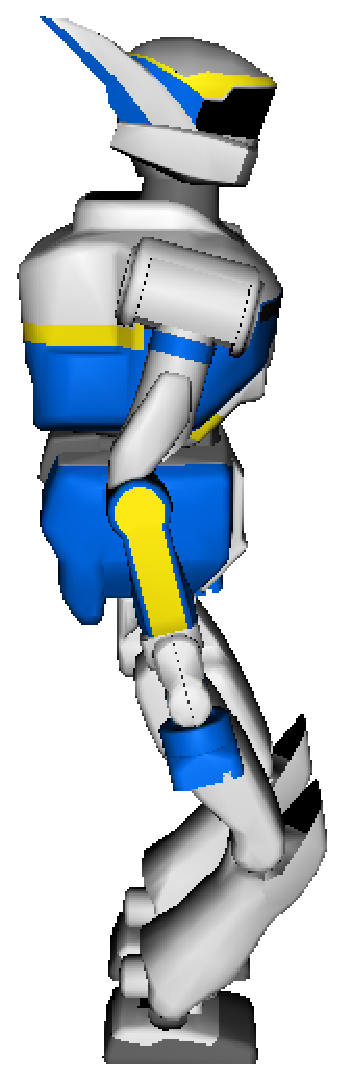
\includegraphics[scale=0.41]{hrp2_side.eps}}
        \subcaption{
            side view
        }
        \label{fig.hrp2_side}
    \end{minipage}
    \hfill
    \begin{minipage}[t]{0.49\textwidth}
        \centering{%
        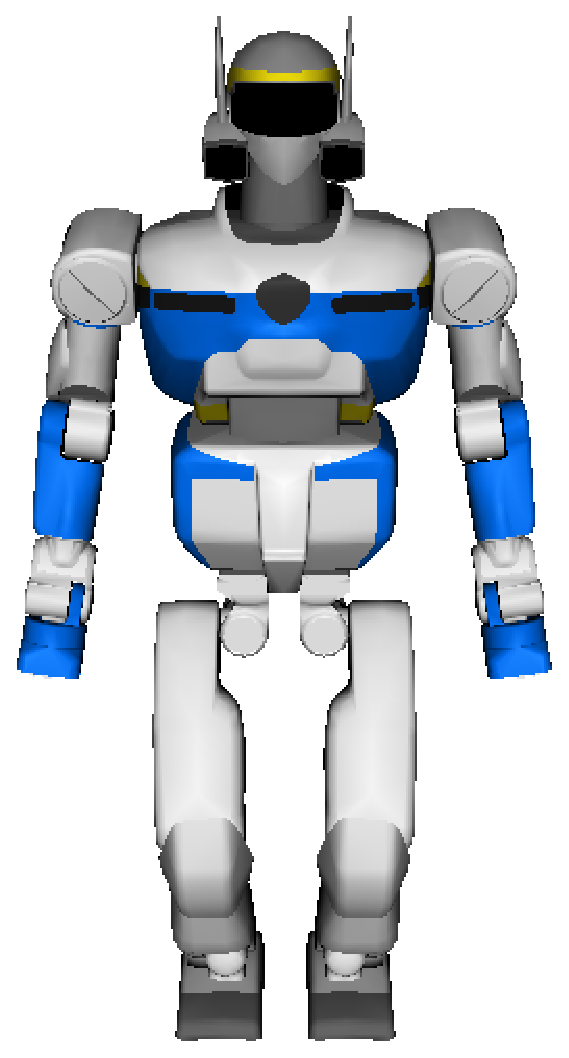
\includegraphics[scale=0.41]{hrp2_front.eps}}
        \subcaption{
            front view
        }
        \label{fig.hrp2_front}
    \end{minipage}
    \caption{
        \sn{HRP-2} robot.
    }
    \label{fig.hrp2}
\end{figure}


Unless stated otherwise, we control and simulate an \sn{HRP-2} robot depicted
in \cref{fig.hrp2} \cite{Kaneko2004icra}. In these cases we assume a perfect
model and perfect inertial measurement unit. The robot has $30$ actuated
joints, its total weight is around $57~[\MT{kg}]$, and the height is around
$1.5~[m]$. The control sampling interval is chosen to be $5~[\MT{ms}]$
($200~[\MT{Hz}]$).



%%%%%%%%%%%%%%%%%%%%%%%%%%%%%%%%%%%%%%%%%%%%%%%%%%%%%%%%%%%%%%%%%%%%%%%%%%%%%%%%
%%%%%%%%%%%%%%%%%%%%%%%%%%%%%%%%%%%%%%%%%%%%%%%%%%%%%%%%%%%%%%%%%%%%%%%%%%%%%%%%
%%%%%%%%%%%%%%%%%%%%%%%%%%%%%%%%%%%%%%%%%%%%%%%%%%%%%%%%%%%%%%%%%%%%%%%%%%%%%%%%
\section{Task-driven walking}\label{sec.task_walk}
\vspace{-1cm}
%
\begin{figure}[!htb]
    \begin{minipage}[t]{0.49\textwidth}
        \centering{
            % Title: glps_renderer figure
% Creator: GL2PS 1.3.8, (C) 1999-2012 C. Geuzaine
% For: Octave
% CreationDate: Mon May  9 19:25:21 2016
\setlength{\unitlength}{0.4pt}
\begin{picture}(0,0)
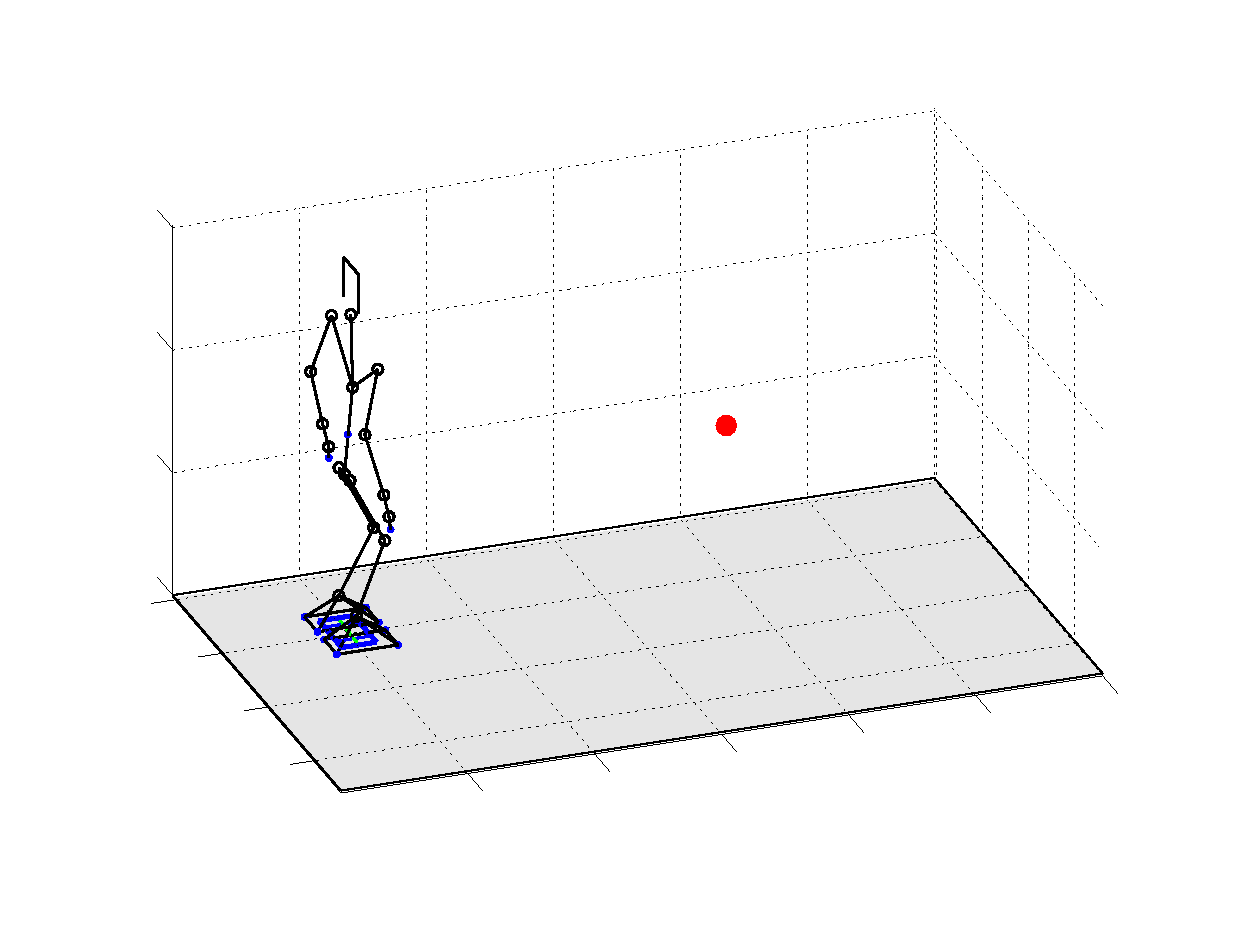
\includegraphics[trim=60  30  50   5,clip,scale=0.4]{test_16_02_robot_1-inc}
\end{picture}%
\begin{picture}(466, 397)(60,30)
\fontsize{7}{0}
\selectfont\put(64.3583,166.387){\makebox(0,0)[br]{\textcolor[rgb]{0,0,0}{{0}}}}
\fontsize{7}{0}
\selectfont\put(64.3583,225.171){\makebox(0,0)[br]{\textcolor[rgb]{0,0,0}{{0.5}}}}
\fontsize{7}{0}
\selectfont\put(64.3583,283.955){\makebox(0,0)[br]{\textcolor[rgb]{0,0,0}{{1}}}}
\fontsize{7}{0}
\selectfont\put(64.3583,342.738){\makebox(0,0)[br]{\textcolor[rgb]{0,0,0}{{1.5}}}}
\fontsize{7}{0}
\selectfont\put(59.8529,149.46){\makebox(0,0)[tr]{\textcolor[rgb]{0,0,0}{{0.5}}}}
\fontsize{7}{0}
\selectfont\put(82.0365,123.702){\makebox(0,0)[tr]{\textcolor[rgb]{0,0,0}{{0}}}}
\fontsize{7}{0}
\selectfont\put(470.853,93.8307){\makebox(0,0)[tl]{\textcolor[rgb]{0,0,0}{{2}}}}
\fontsize{7}{0}
\selectfont\put(531.802,103.206){\makebox(0,0)[tl]{\textcolor[rgb]{0,0,0}{{2.5}}}}
\fontsize{7}{0}
\selectfont\put(104.22,97.9436){\makebox(0,0)[tr]{\textcolor[rgb]{0,0,0}{{-0.5}}}}
\fontsize{7}{0}
\selectfont\put(126.404,72.1854){\makebox(0,0)[tr]{\textcolor[rgb]{0,0,0}{{-1}}}}
\fontsize{7}{0}
\selectfont\put(227.056,56.3298){\makebox(0,0)[tl]{\textcolor[rgb]{0,0,0}{{0}}}}
\fontsize{7}{0}
\selectfont\put(288.005,65.705){\makebox(0,0)[tl]{\textcolor[rgb]{0,0,0}{{0.5}}}}
\fontsize{7}{0}
\selectfont\put(348.954,75.0803){\makebox(0,0)[tl]{\textcolor[rgb]{0,0,0}{{1}}}}
\fontsize{7}{0}
\selectfont\put(409.903,84.4555){\makebox(0,0)[tl]{\textcolor[rgb]{0,0,0}{{1.5}}}}
\end{picture}

            \subcaption{initial}
            \label{fig.task_walk.1}
        }
    \end{minipage}
    \hfill
    \begin{minipage}[t]{0.49\textwidth}
        \centering{
            \input{test_16_02_robot_501.tex}
            \subcaption{after $2.5$ seconds}
            \label{fig.task_walk.2}
        }
    \end{minipage}
    \begin{minipage}[t]{0.49\textwidth}
        \centering{
            \input{test_16_02_robot_1001.tex}
            \subcaption{after $5$ seconds}
            \label{fig.task_walk.3}
        }
    \end{minipage}
    \hfill
    \begin{minipage}[t]{0.49\textwidth}
        \centering{
            \input{test_16_02_robot_1501.tex}
            \subcaption{after $7.5$ seconds}
            \label{fig.task_walk.4}
        }
    \end{minipage}
    \begin{minipage}[t]{0.49\textwidth}
        \centering{
            \input{test_16_02_robot_2001.tex}
            \subcaption{after $10$ seconds}
            \label{fig.task_walk.5}
        }
    \end{minipage}
    \hfill
    \begin{minipage}[t]{0.49\textwidth}
        \centering{
            \input{test_16_02_robot_2501.tex}
            \subcaption{after $12.5$ seconds}
            \label{fig.task_walk.6}
        }
    \end{minipage}
    \caption[Task-driven walk: configurations of the robot during the simulation.]{
        Task-driven walk: configurations of the robot during the simulation.
        Red point indicates position of the target, blue rectangles -- current
        and anticipated positions of the feet.
    }
    \label{fig.task_walk}
\end{figure}
%

It is typical to express high level goals of humanoid robot control using whole
body tasks, execution of which may require locomotion. For example, it might be
necessary to approach an object before grasping it. In such situations it is
necessary to anticipate walking motions taking the whole body tasks into
account. This, however, may not be straightforward when anticipation with an
approximate model is performed, due to simplifications made during the
construction of the model (see \cref{sec.mmpc}). For example, in the case of
point-mass models it is common to map whole body tasks to motions of the
\ac{CoM} or feet \cite{Yoshida2006humanoids, Nishiwaki2003icra,
Fukumoto2004iros, Herdt2010auro}. Such mappings, however, are often task- and
model- specific and their development requires human involvement. \acf{MMPC}
addresses this problem by mixing approximate and whole body models to allow
their automatic interaction without any additional mapping procedures. It also
allows to account for multiple tasks simultaneously in a straightforward way.

%
\begin{figure}[!htb]
    \begin{minipage}[t]{\textwidth}
        \centering{
            \input{steps_16_02_03_N16_nodist.tex}
            \subcaption{without disturbances}
            \label{fig.task_walk_steps.nodist}
        }
    \end{minipage}
    \begin{minipage}[t]{\textwidth}
        \centering{
            % Title: glps_renderer figure
% Creator: GL2PS 1.3.8, (C) 1999-2012 C. Geuzaine
% For: Octave
% CreationDate: Wed Mar 23 18:52:34 2016
\setlength{\unitlength}{0.8pt}
\begin{picture}(0,0)
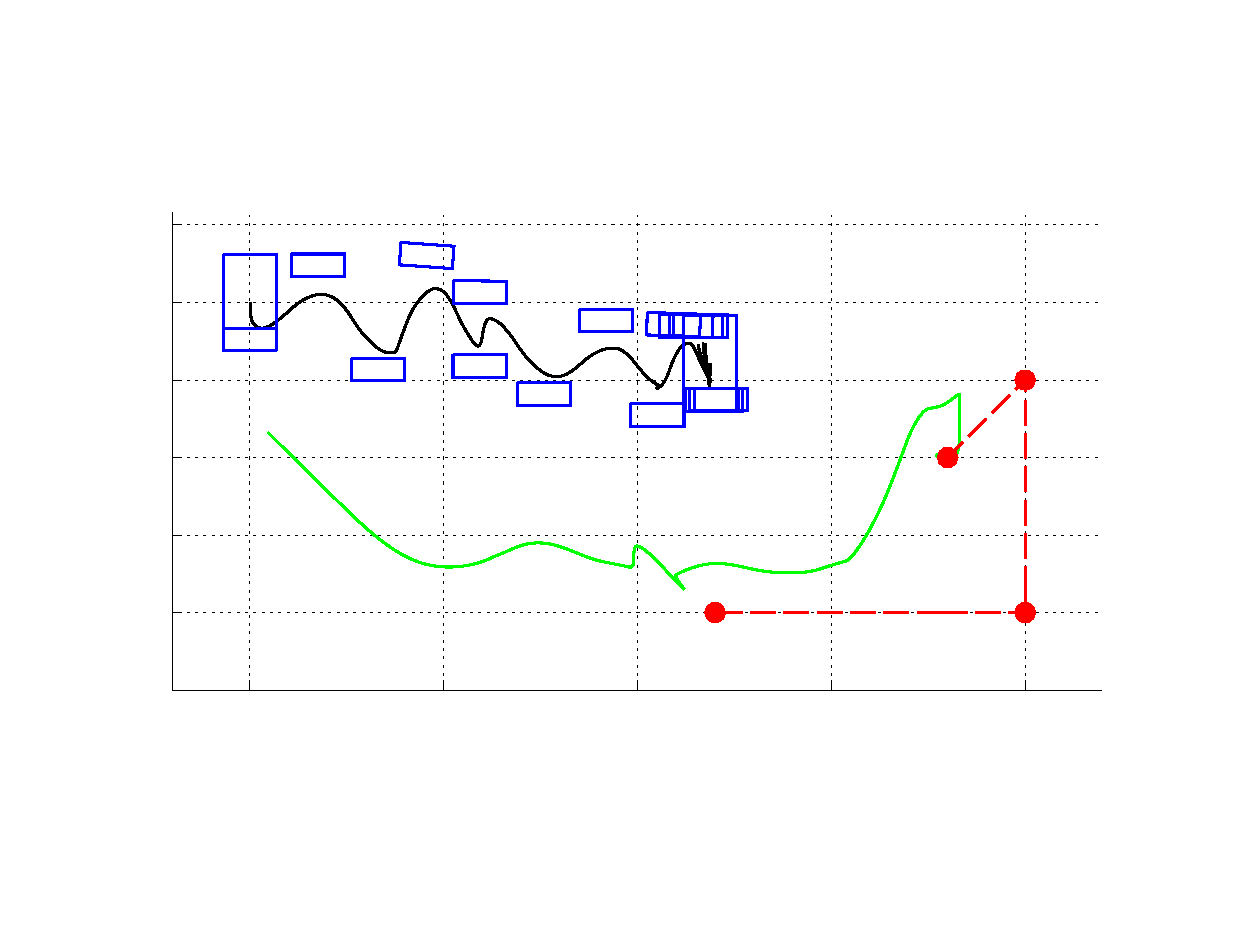
\includegraphics[trim=50  75  50  90,clip,scale=0.8]{steps_16_02_01_N16-inc}
\end{picture}%
\begin{picture}(476, 267)(50,75)
\fontsize{11}{0}
\selectfont\put(111.96,103.583){\makebox(0,0)[t]{\textcolor[rgb]{0,0,0}{{0}}}}
\fontsize{11}{0}
\selectfont\put(204.987,103.583){\makebox(0,0)[t]{\textcolor[rgb]{0,0,0}{{0.5}}}}
\fontsize{11}{0}
\selectfont\put(298.015,103.583){\makebox(0,0)[t]{\textcolor[rgb]{0,0,0}{{1}}}}
\fontsize{11}{0}
\selectfont\put(391.042,103.583){\makebox(0,0)[t]{\textcolor[rgb]{0,0,0}{{1.5}}}}
\fontsize{11}{0}
\selectfont\put(484.069,103.583){\makebox(0,0)[t]{\textcolor[rgb]{0,0,0}{{2}}}}
\fontsize{11}{0}
\selectfont\put(69.8755,108.582){\makebox(0,0)[r]{\textcolor[rgb]{0,0,0}{{-1}}}}
\fontsize{11}{0}
\selectfont\put(69.8755,145.793){\makebox(0,0)[r]{\textcolor[rgb]{0,0,0}{{-0.8}}}}
\fontsize{11}{0}
\selectfont\put(69.8755,183.004){\makebox(0,0)[r]{\textcolor[rgb]{0,0,0}{{-0.6}}}}
\fontsize{11}{0}
\selectfont\put(69.8755,220.215){\makebox(0,0)[r]{\textcolor[rgb]{0,0,0}{{-0.4}}}}
\fontsize{11}{0}
\selectfont\put(69.8755,257.425){\makebox(0,0)[r]{\textcolor[rgb]{0,0,0}{{-0.2}}}}
\fontsize{11}{0}
\selectfont\put(69.8755,294.636){\makebox(0,0)[r]{\textcolor[rgb]{0,0,0}{{0}}}}
\fontsize{11}{0}
\selectfont\put(69.8755,331.847){\makebox(0,0)[r]{\textcolor[rgb]{0,0,0}{{0.2}}}}
\fontsize{11}{0}
\selectfont\put(298.08,87.5828){\makebox(0,0)[t]{\textcolor[rgb]{0,0,0}{{$x~[m]$}}}}
\fontsize{11}{0}
\selectfont\put(40.8755,223.56){\rotatebox{90}{\makebox(0,0)[b]{\textcolor[rgb]{0,0,0}{{$y~[m]$}}}}}
\fontsize{11}{0}
\selectfont\put(344.528,136.49){\makebox(0,0)[l]{\textcolor[rgb]{0,0,0}{{1}}}}
\fontsize{11}{0}
\selectfont\put(493.372,136.49){\makebox(0,0)[l]{\textcolor[rgb]{0,0,0}{{2}}}}
\fontsize{11}{0}
\selectfont\put(493.372,248.123){\makebox(0,0)[l]{\textcolor[rgb]{0,0,0}{{3}}}}
\fontsize{11}{0}
\selectfont\put(456.161,210.912){\makebox(0,0)[l]{\textcolor[rgb]{0,0,0}{{4}}}}
\end{picture}

            \subcaption{with disturbances}
            \label{fig.task_walk_steps.dist}
        }
    \end{minipage}
    \caption[Task-driven walk: top view.]{
        Task-driven walk: top view. Footsteps are represented by rectangles,
        trajectory of the \ac{CoM} is in black, trajectory of the hand is in
        green, while the trajectory of the target is in dashed red. Numbers
        indicate ordering of the target positions.
    }
    \label{fig.task_walk_steps}
\end{figure}
%

The interplay between the models in \ac{MMPC} was shown in
\cite{Sherikov2014humanoids}, where a whole body task induces walking motion.
The task is to reach a varying target point with the right hand of the robot
(see \cref{fig.task_walk,fig.task_walk_steps}). We also demonstrated that this
controller performs automatic repositioning of the feet in order to compensate
for disturbances applied to the robot. We describe this controller and
simulation setting in \cref{sec.task_walk_controller,sec.task_walk_setting}.
The obtained results are discussed in \cref{sec.task_walk_results}.




%%%%%%%%%%%%%%%%%%%%%%%%%%%%%%%%%%%%%%%%%%%%%%%%%%%%%%%%%%%%%%%%%%%%%%%%%%%%%%%%
\subsection{Setting}\label{sec.task_walk_setting}

We evaluate the proposed controller in a simulation, which lasts for
approximately $15$ second. During this time the robot has to reach a target
with its right hand. Initially, the target cannot be reached by the robot while
standing. During the simulation the target is repositioned at $4.6$, $6.25$,
and $8$ second in an unpredictable way (see \cref{fig.task_walk_steps}). In
order to further complicate the task for the controller, we apply disturbances
to the robot at $2.5$ second from the right ($\impulseC_d^y = 15~[\MT{Ns}]$)
and at $7$ second from the front ($\impulseC_d^x = -15~[\MT{Ns}]$). The
disturbances are simulated as described in \cref{app.collision}.


Thus, the goal of the controller is to automatically choose positions of the
feet on the ground in order to reach the target and compensate for
disturbances.



%%%%%%%%%%%%%%%%%%%%%%%%%%%%%%%%%%%%%%%%%%%%%%%%%%%%%%%%%%%%%%%%%%%%%%%%%%%%%%%%
\subsection{Design of the controller}\label{sec.task_walk_controller}


We construct a hierarchy corresponding to \ac{MMPC} controller based on the
whole body (\nameref{model.WB}) and point-mass (\nameref{model.PPMZ}) models as
proposed in \cref{sec.mmpc_hierarchy}. In order to reduce the size of the
\ac{PLLS} problem, we condense \nameref{model.PPMZ} and eliminate torques from
\nameref{model.WB} in advance (see \cref{sec.plls_preprocessing}). This results
in the following hierarchy:
%
\changeHierarchyStyle{breakable,width=14.5cm,before=,after=\par}{\setlength{\itemsep}{5pt}}
\begin{hierarchy}[hr.mmpc_walk]
    \level Simple bounds
            \begin{itemize}%[topsep=3pt]
                \item \makebox[5.2cm][l]{
                        $\displaystyle \ubar{\ddq}^{\prime}  \le  \ddqn  \le  \bar{\ddq}^{\prime}$
                    }
                    $30$ joint limits
                \item \makebox[5.2cm][l]{
                        $\displaystyle \V{\lambda}_i \ge \V{0}$
                    }
                    $3 M$ constraints due to friction cones
                \item \makebox[5.2cm][l]{
                        $\displaystyle \ubarV{\objb}_{\contact,j} \le \Delta\hat{\contact}_{j} \le \barV{\objb}_{\contact,j}$
                    }
                    $2 K$ constraints on foot positions
                \item \makebox[5.2cm][l]{
                        $\displaystyle \ubar{\cop} \le \hat{\cop}_{k+1} \le \bar{\cop}$
                    }
                    $2 N$ constraints on the \acs{CoP} positions
            \end{itemize}

    \level Tasks of the whole body motion controller
            \begin{itemize}%[topsep=3pt]
                \item
                    $\displaystyle
                        \begin{bmatrix}
                            \M{H}_2\\
                            \M{H}_3\\
                        \end{bmatrix}
                        \ddq
                        +
                        \begin{bmatrix}
                            \V{h}_2\\
                            \V{h}_3
                        \end{bmatrix}
                        =
                        m
                        \begin{bmatrix}
                            \T{\Jcom[,2]}\\
                            \T{\Jcom[,3]}
                        \end{bmatrix}
                        \V{g}
                        +
                        \sum_{i=1}^M
                            \begin{bmatrix}
                                \T{\M{J}_{i,2}}\\
                                \T{\M{J}_{i,3}}
                            \end{bmatrix}
                        \begin{bmatrix}
                            \M{V}_i \V{\lambda}_i\\
                            \moment_i
                        \end{bmatrix}
                    $\\[1mm]
                    \makebox[5.2cm][l]{} $6$ equalities due to Newton-Euler equations

                \item
                    $\displaystyle
                    \ubar{\torques}
                    \le
                    \M{H}_1 \ddq  +  \V{h}_1  -  m \T{\Jcom[,1]} \V{g}  -  \sum_{i=1}^M \T{\M{J}_{i,1}}
                    \begin{bmatrix}
                        \M{V}_i \V{\lambda}_i\\
                        \moment_i
                    \end{bmatrix}
                    \le
                    \bar{\torques}
                    $\\[1mm]
                    \makebox[5.2cm][l]{} $30$ bounds on the joint torques

                \item
                    \makebox[5.2cm][l]{
                        $\displaystyle \M{J}_i \ddq + \dotM{J}_i \dq = \V{0}$
                    }
                    $6 M$ equalities due to fixed contacts

                \item
                    \makebox[5.2cm][l]{
                        $\displaystyle
                        \objA_{\moment,i}
                        \begin{bmatrix}
                            \V{\lambda}_i\\
                            \moment_i
                        \end{bmatrix}
                        \ge
                        \ubarV{\objb}_{\moment,i}
                        $
                    }
                    $6 M$ constraints on the contact moments

                \item
                    \makebox[5.2cm][l]{
                        $\displaystyle
                        \Iz \left( \Jcom \ddq + \dJcom \dq \right) = \pi_{\MT{cz}}$
                    }
                    $1$ equality to maintain the \acs{CoM} height
            \end{itemize}

            Coupling with \nameref{model.PPMZ} model
            \begin{itemize}%[topsep=3pt]
                \item
                    \makebox[5.2cm][l]{
                        $\displaystyle
                        \Ixy \left( \Jcom \ddq + \dJcom \dq \right) = \ddotV{c}^{xy}_0$
                    }
                    $2$ equalities due to \acs{CoM} motion

                \item
                    \makebox[5.2cm][l]{
                        $\displaystyle
                        \M{J}_{\TRAN,s} \ddq + \dotM{J}_{\TRAN,s} \dq
                        =
                        \ddotV{s}_{0}
                        %\objA_{\MT{sa}}
                        %\Delta\hat{\contact}_{0}
                        %+
                        %\V{\objb}_{\MT{sa}}
                        $
                    }
                    $3(2-M)$ equalities due to foot motion
            \end{itemize}

    \level Capturability constraint \cref{eq.cop_control_capturability_ctr}
            \begin{itemize}%[topsep=3pt]
                \item
                    \makebox[5.2cm][l]{
                        $\dotV{c}^{xy}_N + \sqrt{\zeta} \ddotV{c}^{xy}_N = \V{0}$
                    }
                    $2$ equalities
            \end{itemize}

    \level Orientations
            \begin{itemize}%[topsep=3pt]
                \item
                    \makebox[4.5cm][l]{
                        $\displaystyle
                        \M{J}_{\ROT,t} \ddq + \dotM{J}_{\ROT,t} \dq
                        =
                        \V{\pi}_t
                        $
                    }
                    $3$ equalities to maintain torso orientation
                \item
                    \makebox[4.5cm][l]{
                        $\displaystyle
                        \M{J}_{\ROT,s} \ddq + \dotM{J}_{\ROT,s} \dq
                        =
                        \V{\pi}_s
                        $
                    }
                    $3(2-M)$ equalities to maintain foot orientation
            \end{itemize}

    \level Whole body tasks
            \begin{itemize}%[topsep=3pt]
                \item
                    \makebox[5.2cm][l]{
                        $\displaystyle
                        \M{J}_{\TRAN,\MT{rh}} \ddq + \dotM{J}_{\TRAN,\MT{rh}} \dq
                        =
                        \V{\pi}_{\MT{rh}}
                        $
                    }
                    $3$ equalities due to the right hand task

                \item
                    \makebox[5.2cm][l]{
                        $
                        \ddqn = \K_{p} (\qn[\DES] - \qn) - \K_{d} \dqn
                        $
                    }
                    $30$ equalities to control the joints
            \end{itemize}

           Anticipation tasks
            \begin{itemize}%[topsep=3pt]
                \item
                    \makebox[5.2cm][l]{
                        $\displaystyle
                        \dddotV{s}^{xy} = \V{0}
                        $
                    }
                    $2 (2-M)$ equalities to minimize foot jerk

                \item
                    \makebox[5.2cm][l]{
                        $\displaystyle
                            \hat{\cop}_{k+1} = \V{0}
                        $
                    }
                    $2 N$ equalities to center \acs{CoP} positions

                \item
                    \makebox[5.2cm][l]{
                        $\displaystyle
                            \dot{\cop}_{k} = \V{0}
                        $
                    }
                    $2 N$ equalities to minimize \acs{CoP} velocities
            \end{itemize}

        \vars{$\x = \left(\ddq, \V{\lambda}_i, \moment_{i}, \ddotV{c}^{xy}_0, \hat{\cop}_{k+1}, \Delta\hat{\contact}_{j}\right)$\\[1mm]
        \makebox[3.3cm]{} with $\quad i \in \{1, ..., M\}$, $\quad k \in \{0, ..., N-1\}$, $\quad j \in \{0, ..., K\}$}%
\end{hierarchy}
\thesisHierarchyStyle{}%
%
where $M \in \{1,2\}$ is the number of foot contacts, $K$ is the number of
varying footstep positions in the preview horizon, $N$ is the length of the
preview horizon. Notation in the hierarchy is the same as in the preceding
chapters with a few additions:
%
\begin{longtable}[l]{@{\extracolsep{0pt}}l @{\extracolsep{1.5cm}}l}
    $\M{J}_{s} = (\M{J}_{\TRAN,s}, \M{J}_{\ROT,s})$     & Jacobian of the foot in the air,\\
    $\M{J}_{\ROT,t}$                                    & rotational Jacobian of the torso,\\
    $\M{J}_{\TRAN,\MT{rh}}$                             & translational Jacobian of the right hand,\\
    $\pi_{\MT{cz}}$, $\V{\pi}_t$, $\V{\pi}_s$, $\V{\pi}_{\MT{rh}}$ & appropriately defined \acs{PD}-controllers,\\
    $\qn[\DES]$                                         & desired joint angles.
\end{longtable}
%
\noindent The decision variables are
%
\begin{itemize}[topsep=0pt,parsep=0pt,itemsep=0pt]
    \item the generalized accelerations $\ddq$,
    \item contact forces represented with $\V{\lambda}_i$ as described in
        \cref{sec.contact_constraints},
    \item contact moments $\moment_{i}$,
    \item current \ac{CoM} acceleration $\ddotV{c}^{xy}_0$ (the reason for this
        is given in \cref{sec.mmpc_horizon}),
    \item anticipated \ac{CoP} positions $\hat{\cop}_{k+1}$ expressed in
        frames fixed to the feet (see \cref{sec.walkmodel}),
    \item distances $\Delta\hat{\contact}_{j}$ between the $j$-th and $j+1$
        steps in the preview horizon (see \cref{sec.walkmodel}).
\end{itemize}
%


Current acceleration and jerk of the foot in the air $\ddotV{s}_{0}$,
$\dddotV{s}^{xy}$; anticipated velocities of the \ac{CoP} $\dot{\cop}_{k}$; and
parts of the final state of the approximate model $(\dotV{c}^{xy}_N$,
$\ddotV{c}^{xy}_N)$ are kept in the hierarchy to simplify presentation. In the
actual controller they are expressed using variables in $\x$ as explained in
\cref{sec.mpc_simple_bounds} and \cref{app.condensing}.


The considered hierarchy contains two more levels compared to the abstract
hierarchy proposed in \cref{sec.mmpc_hierarchy}. The simple bounds are
collected on a separate level since it is necessary for \sn{LexLS} to be able
to exploit their structure. Also, we have chosen to prioritize the tasks
controlling orientations of the torso and foot in the air over the tasks of the
last level. Otherwise, when disturbances are applied, the controller may not be
able to restore correct orientation of the foot before it touches the ground.


Tasks on the final \cref{hr.mmpc_walk.5}-th level of the hierarchy are
incompatible and are weighted with respect to each other. Some of the choices
of the weights are discussed later in this section. All \ac{PD}-controllers
used in the hierarchy are critically damped, their gains are task specific.
$\K_p$ gain in the joint level \ac{PD}-controller is set to zero for the joints
of the legs and right hand.


Approximate \nameref{model.PPMZ} model cannot automatically choose durations of
steps. For this reason, the duration is fixed for all steps to $0.8~[s]$, which
includes transitional double support of $0.1~[s]$ as in \cite{Herdt2010auro}.
In accordance with the same paper, sequence of steps is produced by a simple
state machine, and the preview horizon is sampled using $T_k = 0.1~[s]$.



%%%%%%%%%%%%%%%%%%%%%%%%%%%%%%%%%%%%%%%%%%%%%%%%%%%%%%%%%%%%%%%%%%%%%%%%%%%%%%%%
\subsection{Results and discussion}\label{sec.task_walk_results}

Main results were obtained using \cref{hr.mmpc_walk} with $N = 16$, which
implies that $K \in \{1,2\}$. In other words the controller anticipates for
approximately two steps into the future.


\cref{fig.task_walk_x,fig.task_walk_y,fig.task_walk_steps} illustrate the
ability of the basic version of the controller to automatically position feet
of the robot in order to execute whole body tasks and compensate for
disturbances. In the beginning of the simulation the robot starts walking since
the target is unreachable, and continues to walk until the target is reached,
around 4 second. However, due to a change in the $x$ position of the target,
the walk is resumed. Lateral motion of the target influences the walk in the
same way. Moreover, we can see that the controller immediately reacts to
disturbances and successfully compensates for them by adjusting footsteps in
mid-air (\cref{fig.task_walk_steps_time_x,fig.task_walk_steps_time_y}).
Once the target is reached the robot continues to walk in place.


In the following subsections we discuss computational performance of
\sn{LexLS}, behavior of the controller with a few minor modifications, and the
quality of the generated motions.




%%%%%%%%%%%%%%%%%%%%%%%%%%%%%%%%%%%%%%%%%%%%%%%%%%%%%%%%%%%%%%%%%%%%%%%%%%%%%%%%
\subsubsection{Capturability constraint}\label{sec.walk_capturability}
\vspace{-0.7cm}
%
\begin{figure}[!htb]
    \begin{minipage}[t]{0.49\textwidth}
        \centering{
            \input{test_16_02_robot_notermctr_1.tex}
            \subcaption{initial}
            \label{fig.task_walk_fall.1}
        }
    \end{minipage}
    \hfill
    \begin{minipage}[t]{0.49\textwidth}
        \centering{
            % Title: glps_renderer figure
% Creator: GL2PS 1.3.8, (C) 1999-2012 C. Geuzaine
% For: Octave
% CreationDate: Mon May  9 19:25:07 2016
\setlength{\unitlength}{0.4pt}
\begin{picture}(0,0)
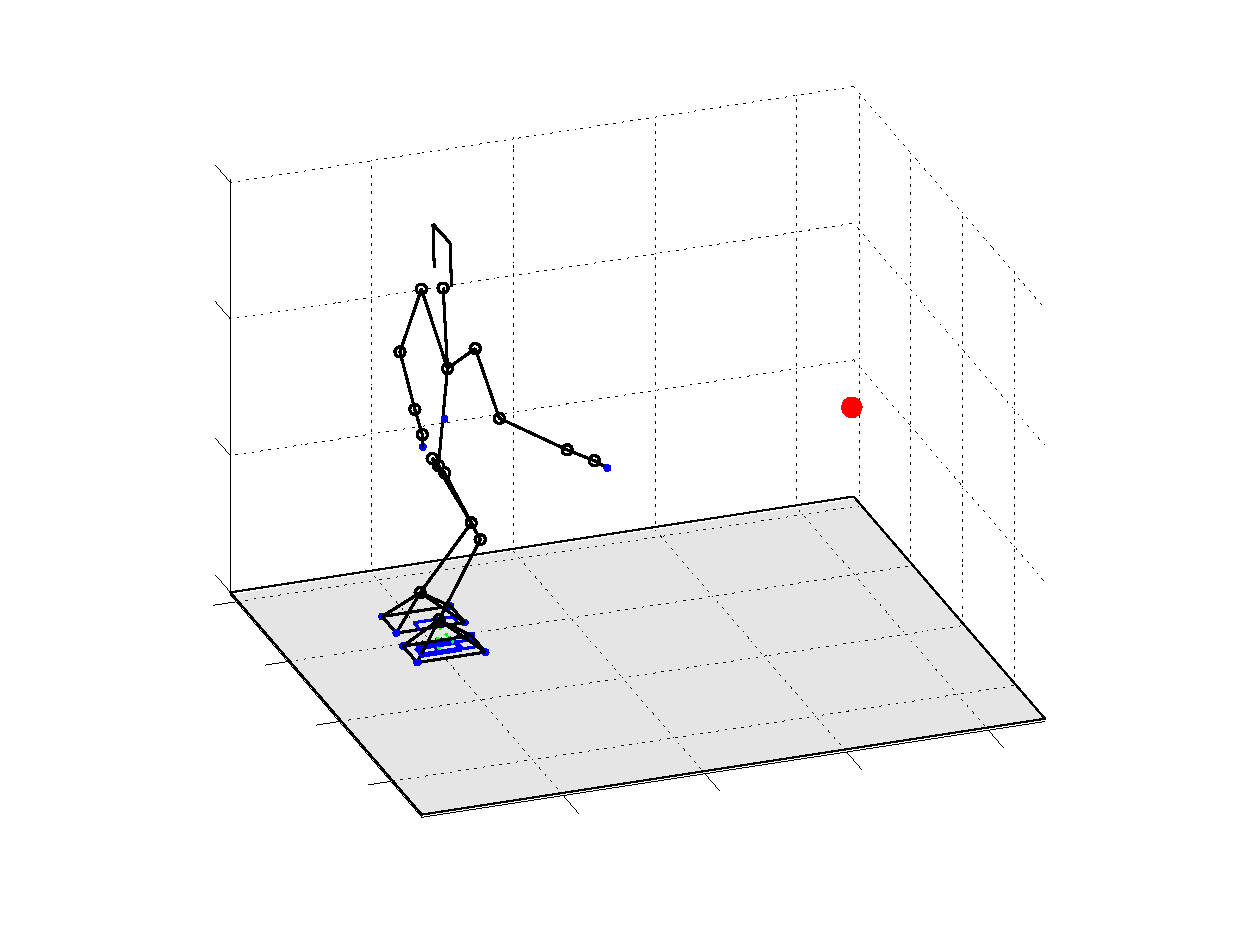
\includegraphics[trim=60  30  50   5,clip,scale=0.4]{test_16_02_robot_notermctr_101-inc}
\end{picture}%
\begin{picture}(466, 397)(60,30)
\fontsize{7}{0}
\selectfont\put(92.0583,167.716){\makebox(0,0)[br]{\textcolor[rgb]{0,0,0}{{0}}}}
\fontsize{7}{0}
\selectfont\put(92.0583,233.307){\makebox(0,0)[br]{\textcolor[rgb]{0,0,0}{{0.5}}}}
\fontsize{7}{0}
\selectfont\put(92.0583,298.899){\makebox(0,0)[br]{\textcolor[rgb]{0,0,0}{{1}}}}
\fontsize{7}{0}
\selectfont\put(92.0583,364.49){\makebox(0,0)[br]{\textcolor[rgb]{0,0,0}{{1.5}}}}
\fontsize{7}{0}
\selectfont\put(89.3552,148.531){\makebox(0,0)[tr]{\textcolor[rgb]{0,0,0}{{0.5}}}}
\fontsize{7}{0}
\selectfont\put(114.108,119.789){\makebox(0,0)[tr]{\textcolor[rgb]{0,0,0}{{0}}}}
\fontsize{7}{0}
\selectfont\put(138.861,91.048){\makebox(0,0)[tr]{\textcolor[rgb]{0,0,0}{{-0.5}}}}
\fontsize{7}{0}
\selectfont\put(163.613,62.3068){\makebox(0,0)[tr]{\textcolor[rgb]{0,0,0}{{-1}}}}
\fontsize{7}{0}
\selectfont\put(272.876,45.7507){\makebox(0,0)[tl]{\textcolor[rgb]{0,0,0}{{0}}}}
\fontsize{7}{0}
\selectfont\put(340.884,56.2116){\makebox(0,0)[tl]{\textcolor[rgb]{0,0,0}{{0.5}}}}
\fontsize{7}{0}
\selectfont\put(408.891,66.6726){\makebox(0,0)[tl]{\textcolor[rgb]{0,0,0}{{1}}}}
\fontsize{7}{0}
\selectfont\put(476.899,77.1335){\makebox(0,0)[tl]{\textcolor[rgb]{0,0,0}{{1.5}}}}
\end{picture}

            \subcaption{after $0.5$ seconds}
            \label{fig.task_walk_fall.2}
        }
    \end{minipage}
    \begin{minipage}[t]{0.49\textwidth}
        \centering{
            \input{test_16_02_robot_notermctr_176.tex}
            \subcaption{after $0.875$ seconds}
            \label{fig.task_walk_fall.3}
        }
    \end{minipage}
    \hfill
    \begin{minipage}[t]{0.49\textwidth}
        \centering{
            \input{test_16_02_robot_notermctr_250.tex}
            \subcaption{after $1.25$ seconds}
            \label{fig.task_walk_fall.4}
        }
    \end{minipage}
    \caption[A fall due to removal of the capturability constraint.]{
        A fall due to removal of the capturability constraint.
    }
    \label{fig.task_walk_fall}
\end{figure}


\begin{figure}[!htbp]
    \begin{minipage}[t]{\textwidth}
        \centering{
            \input{test_16_02_XY_nodist_X_3061.tex}
            \subcaption{$N = 16$, without disturbances}
            \label{fig.task_walk_x_nodist}
        }
    \end{minipage}
    \hfill
    \begin{minipage}[t]{\textwidth}
        \centering{
            \input{test_16_02_XY_X_3061.tex}
            \subcaption{$N = 16$, with disturbances}
            \label{fig.task_walk_x_dist}
        }
    \end{minipage}
    \caption[Reaction to disturbances and changes of the target position ($x$ components).]{
        Evolution of the $x$ components of the target, hand, and current
        support positions and \ac{CoM} velocity with time. The time instants,
        when disturbances are applied, are indicated with vertical dashed black
        lines.
    }
    \label{fig.task_walk_x}
\end{figure}


\begin{figure}[!htbp]
    \begin{minipage}[t]{\textwidth}
        \centering{
            % Title: glps_renderer figure
% Creator: GL2PS 1.3.8, (C) 1999-2012 C. Geuzaine
% For: Octave
% CreationDate: Wed Mar 30 19:27:42 2016
\setlength{\unitlength}{0.7pt}
\begin{picture}(0,0)
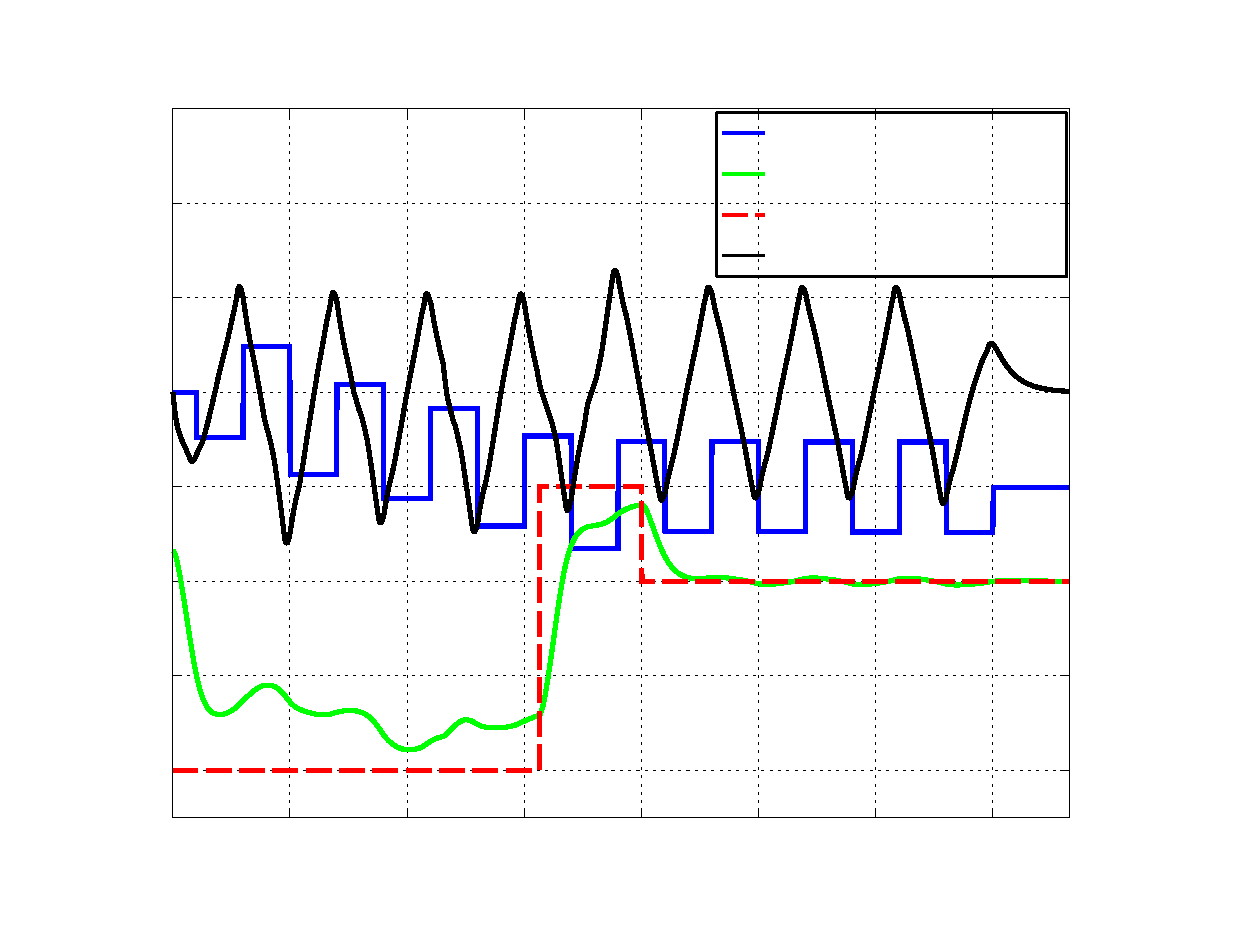
\includegraphics[trim=60   0  60  10,clip,scale=0.7]{test_16_02_XY_nodist_Y_3061-inc}
\end{picture}%
\begin{picture}(456, 422)(60,0)
\fontsize{11}{0}
\selectfont\put(74.88,42.5188){\makebox(0,0)[t]{\textcolor[rgb]{0,0,0}{{0}}}}
\fontsize{11}{0}
\selectfont\put(131.123,42.5188){\makebox(0,0)[t]{\textcolor[rgb]{0,0,0}{{2}}}}
\fontsize{11}{0}
\selectfont\put(187.366,42.5188){\makebox(0,0)[t]{\textcolor[rgb]{0,0,0}{{4}}}}
\fontsize{11}{0}
\selectfont\put(243.609,42.5188){\makebox(0,0)[t]{\textcolor[rgb]{0,0,0}{{6}}}}
\fontsize{11}{0}
\selectfont\put(299.852,42.5188){\makebox(0,0)[t]{\textcolor[rgb]{0,0,0}{{8}}}}
\fontsize{11}{0}
\selectfont\put(356.095,42.5188){\makebox(0,0)[t]{\textcolor[rgb]{0,0,0}{{10}}}}
\fontsize{11}{0}
\selectfont\put(412.338,42.5188){\makebox(0,0)[t]{\textcolor[rgb]{0,0,0}{{12}}}}
\fontsize{11}{0}
\selectfont\put(468.581,42.5188){\makebox(0,0)[t]{\textcolor[rgb]{0,0,0}{{14}}}}
\fontsize{11}{0}
\selectfont\put(69.8753,70.192){\makebox(0,0)[r]{\textcolor[rgb]{0,0,0}{{-0.8}}}}
\fontsize{11}{0}
\selectfont\put(69.8753,115.536){\makebox(0,0)[r]{\textcolor[rgb]{0,0,0}{{-0.6}}}}
\fontsize{11}{0}
\selectfont\put(69.8753,160.88){\makebox(0,0)[r]{\textcolor[rgb]{0,0,0}{{-0.4}}}}
\fontsize{11}{0}
\selectfont\put(69.8753,206.224){\makebox(0,0)[r]{\textcolor[rgb]{0,0,0}{{-0.2}}}}
\fontsize{11}{0}
\selectfont\put(69.8753,251.568){\makebox(0,0)[r]{\textcolor[rgb]{0,0,0}{{0}}}}
\fontsize{11}{0}
\selectfont\put(69.8753,296.912){\makebox(0,0)[r]{\textcolor[rgb]{0,0,0}{{0.2}}}}
\fontsize{11}{0}
\selectfont\put(69.8753,342.256){\makebox(0,0)[r]{\textcolor[rgb]{0,0,0}{{0.4}}}}
\fontsize{11}{0}
\selectfont\put(290.08,31.5188){\makebox(0,0)[t]{\textcolor[rgb]{0,0,0}{{simulation time $[s]$}}}}
\fontsize{11}{0}
\selectfont\put(47.8754,217.56){\rotatebox{90}{\makebox(0,0)[b]{\textcolor[rgb]{0,0,0}{{value along the $y$ axis}}}}}
\fontsize{11}{0}
\selectfont\put(361.461,375.996){\makebox(0,0)[l]{\textcolor[rgb]{0,0,0}{{Current foot position}}}}
\fontsize{11}{0}
\selectfont\put(361.461,356.326){\makebox(0,0)[l]{\textcolor[rgb]{0,0,0}{{Right hand position}}}}
\fontsize{11}{0}
\selectfont\put(361.461,336.657){\makebox(0,0)[l]{\textcolor[rgb]{0,0,0}{{Target position}}}}
\fontsize{11}{0}
\selectfont\put(361.461,316.987){\makebox(0,0)[l]{\textcolor[rgb]{0,0,0}{{CoM velocity}}}}
\end{picture}

            \subcaption{$N = 16$, without disturbances}
            \label{fig.task_walk_y_nodist}
        }
    \end{minipage}
    \hfill
    \begin{minipage}[t]{\textwidth}
        \centering{
            \input{test_16_02_XY_Y_3061.tex}
            \subcaption{$N = 16$, with disturbances}
            \label{fig.task_walk_y_dist}
        }
    \end{minipage}
    \caption[Reaction to disturbances and changes of the target position ($y$ components).]{
        Evolution of the $y$ components of the target, hand, and current
        support positions and \ac{CoM} velocity with time. The time instants,
        when disturbances are applied, are indicated with vertical dashed black
        lines.
    }
    \label{fig.task_walk_y}
\end{figure}


\begin{figure}[!htbp]
    \begin{minipage}[t]{\textwidth}
        \centering{
            % Title: glps_renderer figure
% Creator: GL2PS 1.3.8, (C) 1999-2012 C. Geuzaine
% For: Octave
% CreationDate: Wed Mar 30 19:27:50 2016
\setlength{\unitlength}{0.7pt}
\begin{picture}(0,0)
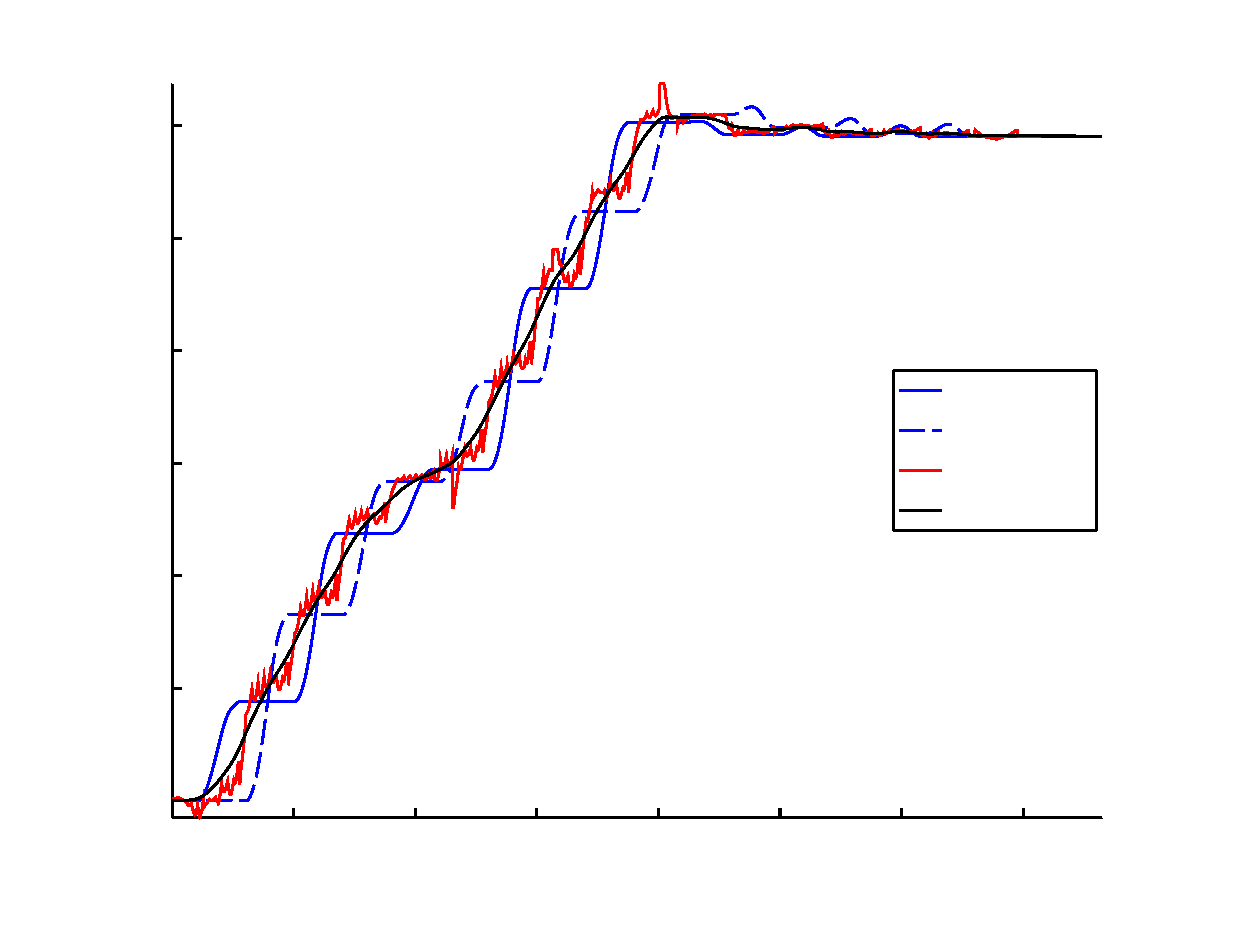
\includegraphics[trim=50   0  50  10,clip,scale=0.7]{steps_time_x_16_02_01_N16_nodist-inc}
\end{picture}%
\begin{picture}(476, 422)(50,0)
\fontsize{11}{0}
\selectfont\put(133.068,42.5189){\makebox(0,0)[t]{\textcolor[rgb]{0,0,0}{{2}}}}
\fontsize{11}{0}
\selectfont\put(191.402,42.5189){\makebox(0,0)[t]{\textcolor[rgb]{0,0,0}{{4}}}}
\fontsize{11}{0}
\selectfont\put(249.736,42.5189){\makebox(0,0)[t]{\textcolor[rgb]{0,0,0}{{6}}}}
\fontsize{11}{0}
\selectfont\put(308.07,42.5189){\makebox(0,0)[t]{\textcolor[rgb]{0,0,0}{{8}}}}
\fontsize{11}{0}
\selectfont\put(366.404,42.5189){\makebox(0,0)[t]{\textcolor[rgb]{0,0,0}{{10}}}}
\fontsize{11}{0}
\selectfont\put(424.737,42.5189){\makebox(0,0)[t]{\textcolor[rgb]{0,0,0}{{12}}}}
\fontsize{11}{0}
\selectfont\put(483.071,42.5189){\makebox(0,0)[t]{\textcolor[rgb]{0,0,0}{{14}}}}
\fontsize{11}{0}
\selectfont\put(69.8755,55.442){\makebox(0,0)[r]{\textcolor[rgb]{0,0,0}{{0}}}}
\fontsize{11}{0}
\selectfont\put(69.8755,109.463){\makebox(0,0)[r]{\textcolor[rgb]{0,0,0}{{0.2}}}}
\fontsize{11}{0}
\selectfont\put(69.8755,163.485){\makebox(0,0)[r]{\textcolor[rgb]{0,0,0}{{0.4}}}}
\fontsize{11}{0}
\selectfont\put(69.8755,217.506){\makebox(0,0)[r]{\textcolor[rgb]{0,0,0}{{0.6}}}}
\fontsize{11}{0}
\selectfont\put(69.8755,271.527){\makebox(0,0)[r]{\textcolor[rgb]{0,0,0}{{0.8}}}}
\fontsize{11}{0}
\selectfont\put(69.8755,325.549){\makebox(0,0)[r]{\textcolor[rgb]{0,0,0}{{1}}}}
\fontsize{11}{0}
\selectfont\put(69.8755,379.57){\makebox(0,0)[r]{\textcolor[rgb]{0,0,0}{{1.2}}}}
\fontsize{11}{0}
\selectfont\put(298.08,22.5189){\makebox(0,0)[t]{\textcolor[rgb]{0,0,0}{{simulation time $[s]$}}}}
\fontsize{11}{0}
\selectfont\put(40.8755,223.56){\rotatebox{90}{\makebox(0,0)[b]{\textcolor[rgb]{0,0,0}{{position along the $x$ axis $[m]$}}}}}
\fontsize{11}{0}
\selectfont\put(446.874,252.364){\makebox(0,0)[l]{\textcolor[rgb]{0,0,0}{{Left foot}}}}
\fontsize{11}{0}
\selectfont\put(446.874,233.161){\makebox(0,0)[l]{\textcolor[rgb]{0,0,0}{{Right foot}}}}
\fontsize{11}{0}
\selectfont\put(446.874,213.959){\makebox(0,0)[l]{\textcolor[rgb]{0,0,0}{{CoP}}}}
\fontsize{11}{0}
\selectfont\put(446.874,194.756){\makebox(0,0)[l]{\textcolor[rgb]{0,0,0}{{CoM}}}}
\end{picture}

            \subcaption{$N = 16$, without disturbances}
            \label{fig.task_walk_steps_time_x.nodist}
        }
    \end{minipage}
    \begin{minipage}[t]{\textwidth}
        \centering{
            % Title: glps_renderer figure
% Creator: GL2PS 1.3.8, (C) 1999-2012 C. Geuzaine
% For: Octave
% CreationDate: Wed Mar 30 19:27:48 2016
\setlength{\unitlength}{0.7pt}
\begin{picture}(0,0)
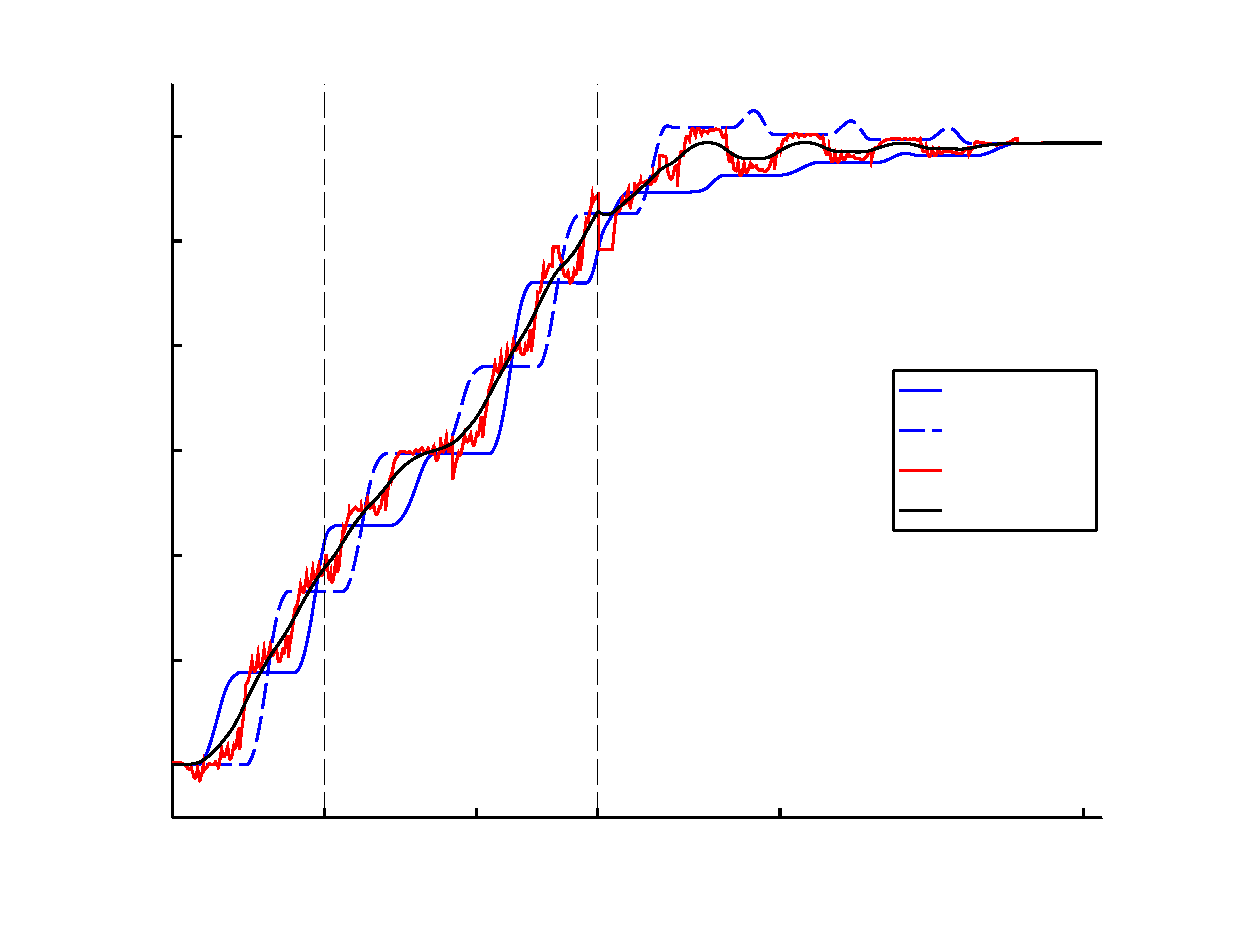
\includegraphics[trim=50   0  50  10,clip,scale=0.7]{steps_time_x_16_02_01_N16-inc}
\end{picture}%
\begin{picture}(476, 422)(50,0)
\fontsize{11}{0}
\selectfont\put(147.652,42.5189){\makebox(0,0)[t]{\textcolor[rgb]{0,0,0}{{$\impulseC_d^y$}}}}
\fontsize{11}{0}
\selectfont\put(220.569,42.5189){\makebox(0,0)[t]{\textcolor[rgb]{0,0,0}{{5}}}}
\fontsize{11}{0}
\selectfont\put(278.903,42.5189){\makebox(0,0)[t]{\textcolor[rgb]{0,0,0}{{$\impulseC_d^x$}}}}
\fontsize{11}{0}
\selectfont\put(366.404,42.5189){\makebox(0,0)[t]{\textcolor[rgb]{0,0,0}{{10}}}}
\fontsize{11}{0}
\selectfont\put(512.238,42.5189){\makebox(0,0)[t]{\textcolor[rgb]{0,0,0}{{15}}}}
\fontsize{11}{0}
\selectfont\put(69.8755,72.6686){\makebox(0,0)[r]{\textcolor[rgb]{0,0,0}{{0}}}}
\fontsize{11}{0}
\selectfont\put(69.8755,122.966){\makebox(0,0)[r]{\textcolor[rgb]{0,0,0}{{0.2}}}}
\fontsize{11}{0}
\selectfont\put(69.8755,173.263){\makebox(0,0)[r]{\textcolor[rgb]{0,0,0}{{0.4}}}}
\fontsize{11}{0}
\selectfont\put(69.8755,223.56){\makebox(0,0)[r]{\textcolor[rgb]{0,0,0}{{0.6}}}}
\fontsize{11}{0}
\selectfont\put(69.8755,273.857){\makebox(0,0)[r]{\textcolor[rgb]{0,0,0}{{0.8}}}}
\fontsize{11}{0}
\selectfont\put(69.8755,324.154){\makebox(0,0)[r]{\textcolor[rgb]{0,0,0}{{1}}}}
\fontsize{11}{0}
\selectfont\put(69.8755,374.451){\makebox(0,0)[r]{\textcolor[rgb]{0,0,0}{{1.2}}}}
\fontsize{11}{0}
\selectfont\put(298.08,22.5189){\makebox(0,0)[t]{\textcolor[rgb]{0,0,0}{{simulation time $[s]$}}}}
\fontsize{11}{0}
\selectfont\put(40.8755,223.56){\rotatebox{90}{\makebox(0,0)[b]{\textcolor[rgb]{0,0,0}{{position along the $x$ axis $[m]$}}}}}
\fontsize{11}{0}
\selectfont\put(446.874,252.364){\makebox(0,0)[l]{\textcolor[rgb]{0,0,0}{{Left foot}}}}
\fontsize{11}{0}
\selectfont\put(446.874,233.161){\makebox(0,0)[l]{\textcolor[rgb]{0,0,0}{{Right foot}}}}
\fontsize{11}{0}
\selectfont\put(446.874,213.959){\makebox(0,0)[l]{\textcolor[rgb]{0,0,0}{{CoP}}}}
\fontsize{11}{0}
\selectfont\put(446.874,194.756){\makebox(0,0)[l]{\textcolor[rgb]{0,0,0}{{CoM}}}}
\end{picture}

            \subcaption{$N = 16$, with disturbances}
            \label{fig.task_walk_steps_time_x.dist}
        }
    \end{minipage}
    \caption[Evolution of the feet, CoM, and CoP positions with time along the $x$ axis.]{
        Evolution of the positions of feet, \ac{CoM}, and \ac{CoP} with time
        along the $x$ axis. The time instants, when disturbances are applied,
        are indicated with vertical dashed black lines.
    }
    \label{fig.task_walk_steps_time_x}
\end{figure}


\begin{figure}[!htbp]
    \begin{minipage}[t]{\textwidth}
        \centering{
            % Title: glps_renderer figure
% Creator: GL2PS 1.3.8, (C) 1999-2012 C. Geuzaine
% For: Octave
% CreationDate: Wed Mar 30 19:27:51 2016
\setlength{\unitlength}{0.7pt}
\begin{picture}(0,0)
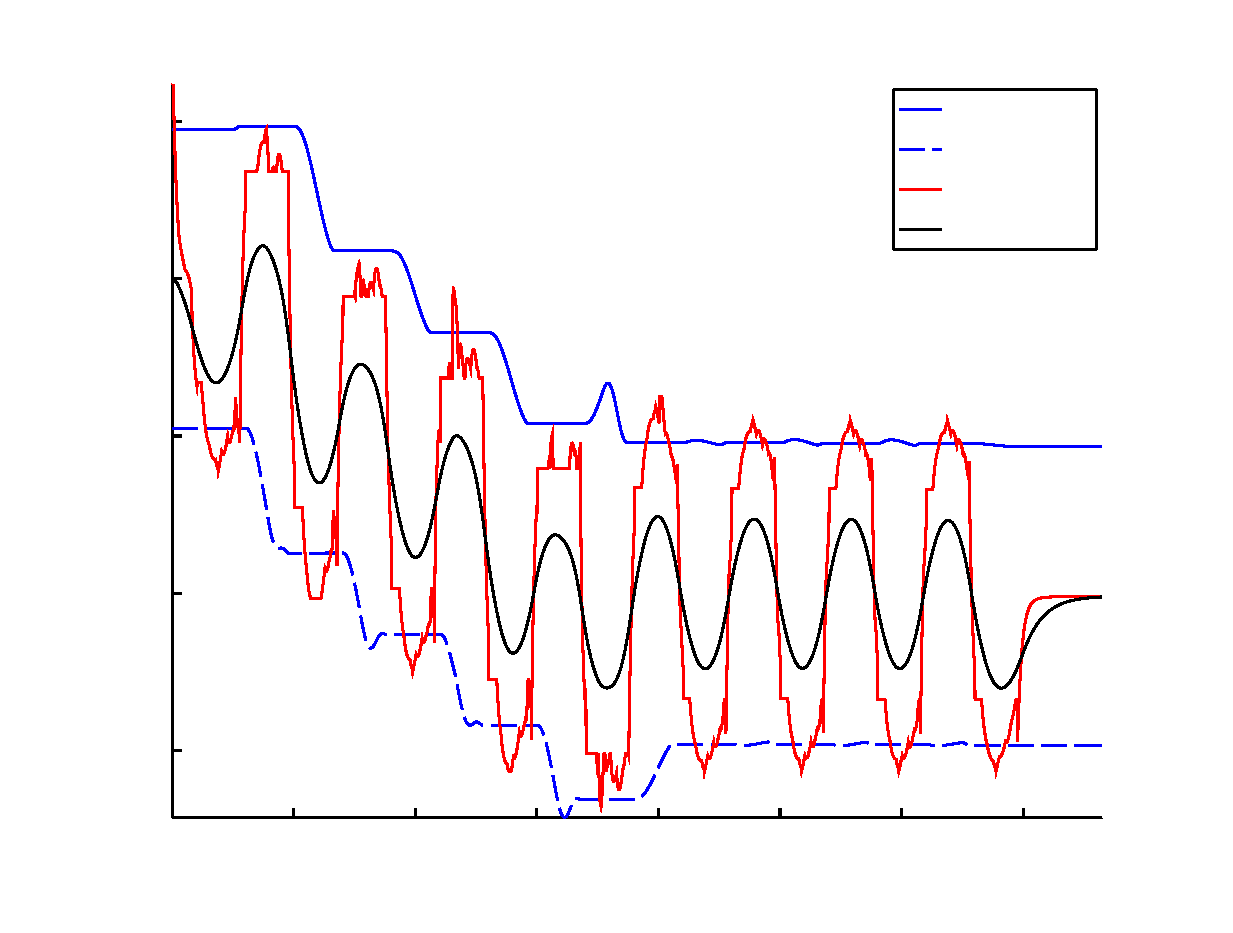
\includegraphics[trim=50   0  50  10,clip,scale=0.7]{steps_time_y_16_02_01_N16_nodist-inc}
\end{picture}%
\begin{picture}(476, 422)(50,0)
\fontsize{11}{0}
\selectfont\put(133.068,42.5189){\makebox(0,0)[t]{\textcolor[rgb]{0,0,0}{{2}}}}
\fontsize{11}{0}
\selectfont\put(191.402,42.5189){\makebox(0,0)[t]{\textcolor[rgb]{0,0,0}{{4}}}}
\fontsize{11}{0}
\selectfont\put(249.736,42.5189){\makebox(0,0)[t]{\textcolor[rgb]{0,0,0}{{6}}}}
\fontsize{11}{0}
\selectfont\put(308.07,42.5189){\makebox(0,0)[t]{\textcolor[rgb]{0,0,0}{{8}}}}
\fontsize{11}{0}
\selectfont\put(366.404,42.5189){\makebox(0,0)[t]{\textcolor[rgb]{0,0,0}{{10}}}}
\fontsize{11}{0}
\selectfont\put(424.737,42.5189){\makebox(0,0)[t]{\textcolor[rgb]{0,0,0}{{12}}}}
\fontsize{11}{0}
\selectfont\put(483.071,42.5189){\makebox(0,0)[t]{\textcolor[rgb]{0,0,0}{{14}}}}
\fontsize{11}{0}
\selectfont\put(69.8755,79.6517){\makebox(0,0)[r]{\textcolor[rgb]{0,0,0}{{-0.3}}}}
\fontsize{11}{0}
\selectfont\put(69.8755,155.111){\makebox(0,0)[r]{\textcolor[rgb]{0,0,0}{{-0.2}}}}
\fontsize{11}{0}
\selectfont\put(69.8755,230.571){\makebox(0,0)[r]{\textcolor[rgb]{0,0,0}{{-0.1}}}}
\fontsize{11}{0}
\selectfont\put(69.8755,306.03){\makebox(0,0)[r]{\textcolor[rgb]{0,0,0}{{0}}}}
\fontsize{11}{0}
\selectfont\put(69.8755,381.489){\makebox(0,0)[r]{\textcolor[rgb]{0,0,0}{{0.1}}}}
\fontsize{11}{0}
\selectfont\put(298.08,22.5189){\makebox(0,0)[t]{\textcolor[rgb]{0,0,0}{{simulation time $[s]$}}}}
\fontsize{11}{0}
\selectfont\put(34.8755,223.56){\rotatebox{90}{\makebox(0,0)[b]{\textcolor[rgb]{0,0,0}{{position along the $y$ axis $[m]$}}}}}
\fontsize{11}{0}
\selectfont\put(446.874,387.253){\makebox(0,0)[l]{\textcolor[rgb]{0,0,0}{{Left foot}}}}
\fontsize{11}{0}
\selectfont\put(446.874,368.05){\makebox(0,0)[l]{\textcolor[rgb]{0,0,0}{{Right foot}}}}
\fontsize{11}{0}
\selectfont\put(446.874,348.847){\makebox(0,0)[l]{\textcolor[rgb]{0,0,0}{{CoP}}}}
\fontsize{11}{0}
\selectfont\put(446.874,329.644){\makebox(0,0)[l]{\textcolor[rgb]{0,0,0}{{CoM}}}}
\end{picture}

            \subcaption{$N = 16$, without disturbances}
            \label{fig.task_walk_steps_time_y.nodist}
        }
    \end{minipage}
    \begin{minipage}[t]{\textwidth}
        \centering{
            % Title: glps_renderer figure
% Creator: GL2PS 1.3.8, (C) 1999-2012 C. Geuzaine
% For: Octave
% CreationDate: Wed Mar 30 19:27:48 2016
\setlength{\unitlength}{0.7pt}
\begin{picture}(0,0)
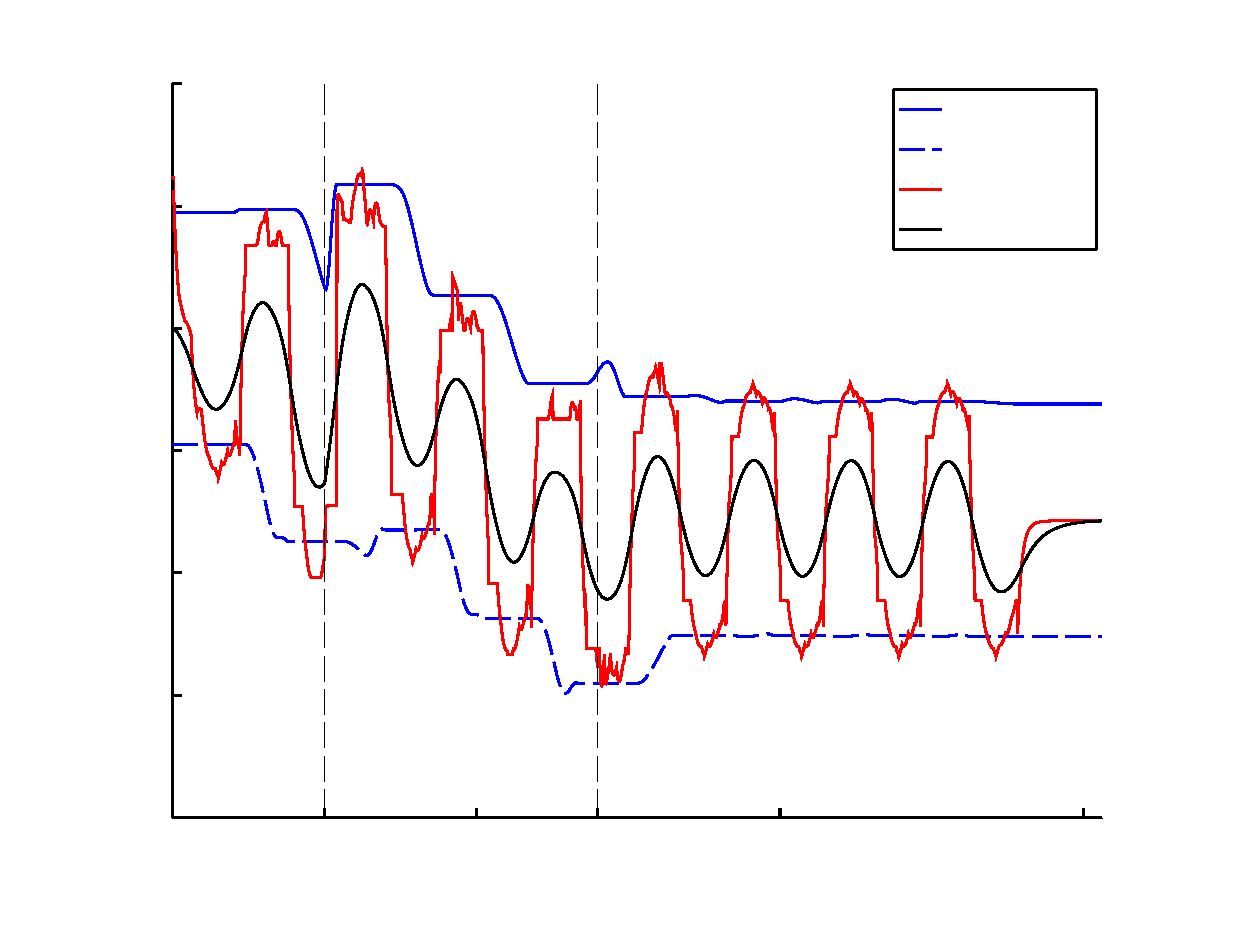
\includegraphics[trim=50   0  50  10,clip,scale=0.7]{steps_time_y_16_02_01_N16-inc}
\end{picture}%
\begin{picture}(476, 422)(50,0)
\fontsize{11}{0}
\selectfont\put(147.652,42.5189){\makebox(0,0)[t]{\textcolor[rgb]{0,0,0}{{$\impulseC_d^y$}}}}
\fontsize{11}{0}
\selectfont\put(220.569,42.5189){\makebox(0,0)[t]{\textcolor[rgb]{0,0,0}{{5}}}}
\fontsize{11}{0}
\selectfont\put(278.903,42.5189){\makebox(0,0)[t]{\textcolor[rgb]{0,0,0}{{$\impulseC_d^x$}}}}
\fontsize{11}{0}
\selectfont\put(366.404,42.5189){\makebox(0,0)[t]{\textcolor[rgb]{0,0,0}{{10}}}}
\fontsize{11}{0}
\selectfont\put(512.238,42.5189){\makebox(0,0)[t]{\textcolor[rgb]{0,0,0}{{15}}}}
\fontsize{11}{0}
\selectfont\put(69.8755,47.52){\makebox(0,0)[r]{\textcolor[rgb]{0,0,0}{{-0.4}}}}
\fontsize{11}{0}
\selectfont\put(69.8755,106.2){\makebox(0,0)[r]{\textcolor[rgb]{0,0,0}{{-0.3}}}}
\fontsize{11}{0}
\selectfont\put(69.8755,164.88){\makebox(0,0)[r]{\textcolor[rgb]{0,0,0}{{-0.2}}}}
\fontsize{11}{0}
\selectfont\put(69.8755,223.56){\makebox(0,0)[r]{\textcolor[rgb]{0,0,0}{{-0.1}}}}
\fontsize{11}{0}
\selectfont\put(69.8755,282.24){\makebox(0,0)[r]{\textcolor[rgb]{0,0,0}{{0}}}}
\fontsize{11}{0}
\selectfont\put(69.8755,340.92){\makebox(0,0)[r]{\textcolor[rgb]{0,0,0}{{0.1}}}}
\fontsize{11}{0}
\selectfont\put(69.8755,399.6){\makebox(0,0)[r]{\textcolor[rgb]{0,0,0}{{0.2}}}}
\fontsize{11}{0}
\selectfont\put(298.08,22.5189){\makebox(0,0)[t]{\textcolor[rgb]{0,0,0}{{simulation time $[s]$}}}}
\fontsize{11}{0}
\selectfont\put(34.8755,223.56){\rotatebox{90}{\makebox(0,0)[b]{\textcolor[rgb]{0,0,0}{{position along the $y$ axis $[m]$}}}}}
\fontsize{11}{0}
\selectfont\put(446.874,387.253){\makebox(0,0)[l]{\textcolor[rgb]{0,0,0}{{Left foot}}}}
\fontsize{11}{0}
\selectfont\put(446.874,368.05){\makebox(0,0)[l]{\textcolor[rgb]{0,0,0}{{Right foot}}}}
\fontsize{11}{0}
\selectfont\put(446.874,348.847){\makebox(0,0)[l]{\textcolor[rgb]{0,0,0}{{CoP}}}}
\fontsize{11}{0}
\selectfont\put(446.874,329.644){\makebox(0,0)[l]{\textcolor[rgb]{0,0,0}{{CoM}}}}
\end{picture}

            \subcaption{$N = 16$, with disturbances}
            \label{fig.task_walk_steps_time_y.dist}
        }
    \end{minipage}
    \caption[Evolution of the feet, CoM, and CoP positions with time along the $y$ axis.]{
        Evolution of the positions of feet, \ac{CoM}, and \ac{CoP} with time
        along the $y$ axis. The time instants, when disturbances are applied,
        are indicated with vertical dashed black lines.
    }
    \label{fig.task_walk_steps_time_y}
\end{figure}


Balanced walking motions can be obtained without a capturability constraint
provided that the weights of the objectives are properly tuned
\cite{Wieber2008iros,Herdt2010auro}. However, addition of such constraint makes
controller less sensitive to the weights. For example, the considered \ac{MMPC}
controller makes the robot fall in the very beginning of the simulation, when
the capturability constraint is omitted (see \cref{fig.task_walk_fall}).
Though, it is possible to adjust objectives on the last level of the hierarchy
and their weights to avoid this, it is unnecessary due to the capturability
constraint.


Satisfaction of the capturability constraint, however, does not guarantee that
the balance is always preserved. We observed that introduction of an additional
level in the hierarchy in order to prioritize the hand task over other tasks of
the last level leads to violent motions of the upper body and, eventually, to a
fall. We believe that the reason for this is that the point-mass approximation
does not reflect the complex dynamics of the robot to a necessary extent.
Hence, approximate models including angular momentum may be more appropriate
for the considered setting.




%%%%%%%%%%%%%%%%%%%%%%%%%%%%%%%%%%%%%%%%%%%%%%%%%%%%%%%%%%%%%%%%%%%%%%%%%%%%%%%%
\subsubsection{Computational performance of \sn{LexLS}}\label{sec.walk_performance}

\vspace{-0.5cm}
\begin{figure*}[!htb]
    \begin{minipage}[t]{0.49\textwidth}
        \centering{
            % Title: glps_renderer figure
% Creator: GL2PS 1.3.8, (C) 1999-2012 C. Geuzaine
% For: Octave
% CreationDate: Wed Mar 23 19:36:50 2016
\setlength{\unitlength}{0.42pt}
\begin{picture}(0,0)
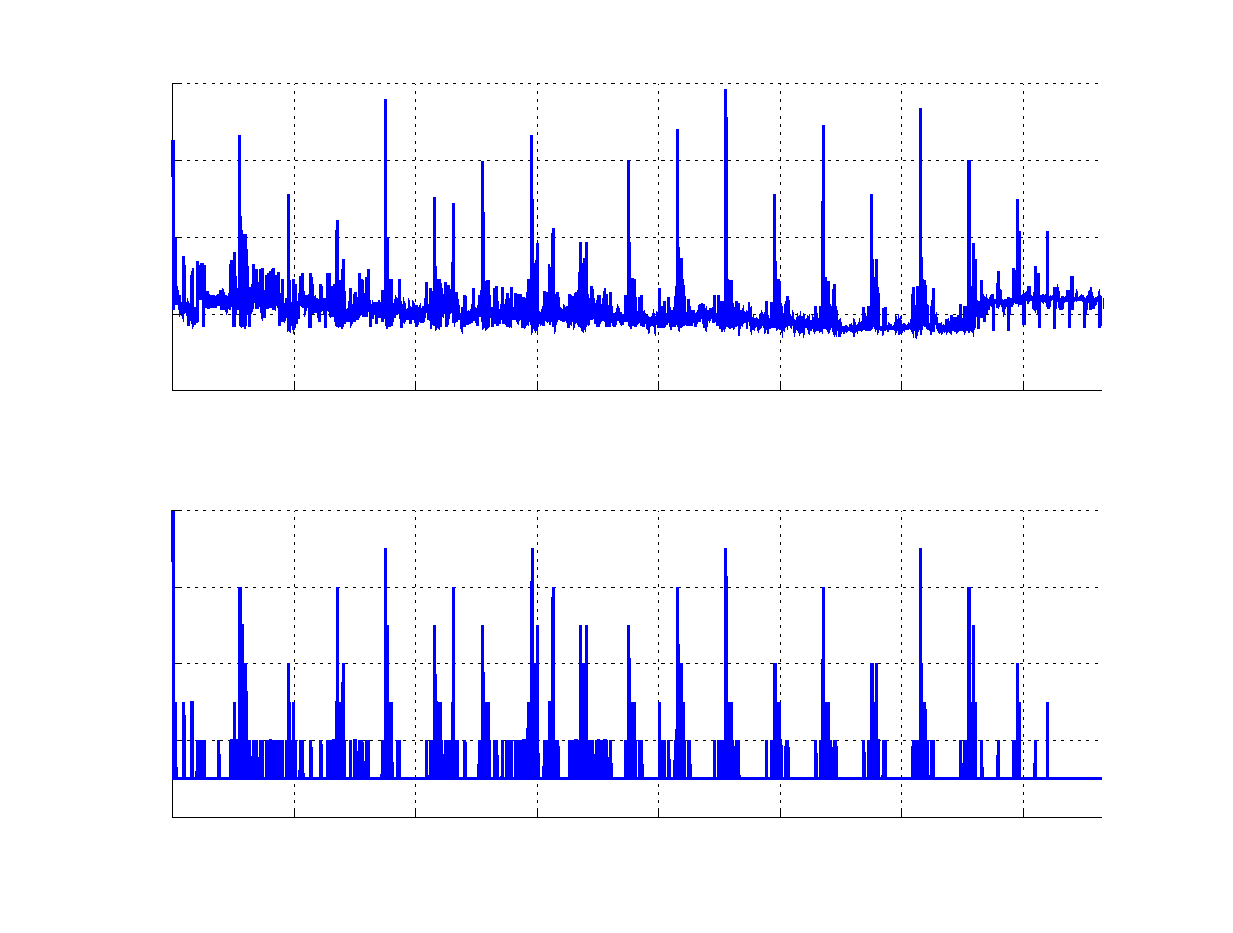
\includegraphics[trim=30  20   0   0,clip,scale=0.42]{time_16_02_03_N16_nodist-inc}
\end{picture}%
\begin{picture}(546, 412)(30,20)
\fontsize{8}{0}
\selectfont\put(74.88,247.205){\makebox(0,0)[t]{\textcolor[rgb]{0,0,0}{{0}}}}
\fontsize{8}{0}
\selectfont\put(133.214,247.205){\makebox(0,0)[t]{\textcolor[rgb]{0,0,0}{{2}}}}
\fontsize{8}{0}
\selectfont\put(191.548,247.205){\makebox(0,0)[t]{\textcolor[rgb]{0,0,0}{{4}}}}
\fontsize{8}{0}
\selectfont\put(249.882,247.205){\makebox(0,0)[t]{\textcolor[rgb]{0,0,0}{{6}}}}
\fontsize{8}{0}
\selectfont\put(308.216,247.205){\makebox(0,0)[t]{\textcolor[rgb]{0,0,0}{{8}}}}
\fontsize{8}{0}
\selectfont\put(366.549,247.205){\makebox(0,0)[t]{\textcolor[rgb]{0,0,0}{{10}}}}
\fontsize{8}{0}
\selectfont\put(424.883,247.205){\makebox(0,0)[t]{\textcolor[rgb]{0,0,0}{{12}}}}
\fontsize{8}{0}
\selectfont\put(483.217,247.205){\makebox(0,0)[t]{\textcolor[rgb]{0,0,0}{{14}}}}
\fontsize{8}{0}
\selectfont\put(69.8755,252.218){\makebox(0,0)[r]{\textcolor[rgb]{0,0,0}{{0}}}}
\fontsize{8}{0}
\selectfont\put(69.8755,289.063){\makebox(0,0)[r]{\textcolor[rgb]{0,0,0}{{1}}}}
\fontsize{8}{0}
\selectfont\put(69.8755,325.909){\makebox(0,0)[r]{\textcolor[rgb]{0,0,0}{{2}}}}
\fontsize{8}{0}
\selectfont\put(69.8755,362.754){\makebox(0,0)[r]{\textcolor[rgb]{0,0,0}{{3}}}}
\fontsize{8}{0}
\selectfont\put(69.8755,399.6){\makebox(0,0)[r]{\textcolor[rgb]{0,0,0}{{4}}}}
\fontsize{8}{0}
\selectfont\put(48.8755,325.909){\rotatebox{90}{\makebox(0,0)[b]{\textcolor[rgb]{0,0,0}{{comp. time $[ms]$}}}}}
\fontsize{8}{0}
\selectfont\put(74.88,42.507){\makebox(0,0)[t]{\textcolor[rgb]{0,0,0}{{0}}}}
\fontsize{8}{0}
\selectfont\put(133.214,42.507){\makebox(0,0)[t]{\textcolor[rgb]{0,0,0}{{2}}}}
\fontsize{8}{0}
\selectfont\put(191.548,42.507){\makebox(0,0)[t]{\textcolor[rgb]{0,0,0}{{4}}}}
\fontsize{8}{0}
\selectfont\put(249.882,42.507){\makebox(0,0)[t]{\textcolor[rgb]{0,0,0}{{6}}}}
\fontsize{8}{0}
\selectfont\put(308.216,42.507){\makebox(0,0)[t]{\textcolor[rgb]{0,0,0}{{8}}}}
\fontsize{8}{0}
\selectfont\put(366.549,42.507){\makebox(0,0)[t]{\textcolor[rgb]{0,0,0}{{10}}}}
\fontsize{8}{0}
\selectfont\put(424.883,42.507){\makebox(0,0)[t]{\textcolor[rgb]{0,0,0}{{12}}}}
\fontsize{8}{0}
\selectfont\put(483.217,42.507){\makebox(0,0)[t]{\textcolor[rgb]{0,0,0}{{14}}}}
\fontsize{8}{0}
\selectfont\put(69.8755,47.52){\makebox(0,0)[r]{\textcolor[rgb]{0,0,0}{{0}}}}
\fontsize{8}{0}
\selectfont\put(69.8755,84.3656){\makebox(0,0)[r]{\textcolor[rgb]{0,0,0}{{2}}}}
\fontsize{8}{0}
\selectfont\put(69.8755,121.211){\makebox(0,0)[r]{\textcolor[rgb]{0,0,0}{{4}}}}
\fontsize{8}{0}
\selectfont\put(69.8755,158.057){\makebox(0,0)[r]{\textcolor[rgb]{0,0,0}{{6}}}}
\fontsize{8}{0}
\selectfont\put(69.8755,194.902){\makebox(0,0)[r]{\textcolor[rgb]{0,0,0}{{8}}}}
\fontsize{8}{0}
\selectfont\put(298.08,9.50697){\makebox(0,0)[t]{\textcolor[rgb]{0,0,0}{{simulation time $[s]$}}}}
\fontsize{8}{0}
\selectfont\put(48.8755,121.211){\rotatebox{90}{\makebox(0,0)[b]{\textcolor[rgb]{0,0,0}{{num. of iterations}}}}}
\end{picture}

            \subcaption{
                $N = 16$, without disturbances.\\
                Mean computational time: $1.04~[\MT{ms}]$.\\
                Time measurements $> 1~[\MT{ms}]$: 49\%
            }
            \label{fig.task_walk_time.1}
        }
    \end{minipage}
    \hfill
    \begin{minipage}[t]{0.49\textwidth}
        \centering{
            \input{time_16_02_01_N16.tex}
            \subcaption{
                $N = 16$, with disturbances.\\
                Mean computational time: $1.09~[\MT{ms}]$.\\
                Time measurements $> 1~[\MT{ms}]$: 62\%
            }
            \label{fig.task_walk_time.2}
        }
    \end{minipage}
    \begin{minipage}[t]{0.49\textwidth}
        \centering{
            % Title: glps_renderer figure
% Creator: GL2PS 1.3.8, (C) 1999-2012 C. Geuzaine
% For: Octave
% CreationDate: Wed Mar 23 19:36:51 2016
\setlength{\unitlength}{0.42pt}
\begin{picture}(0,0)
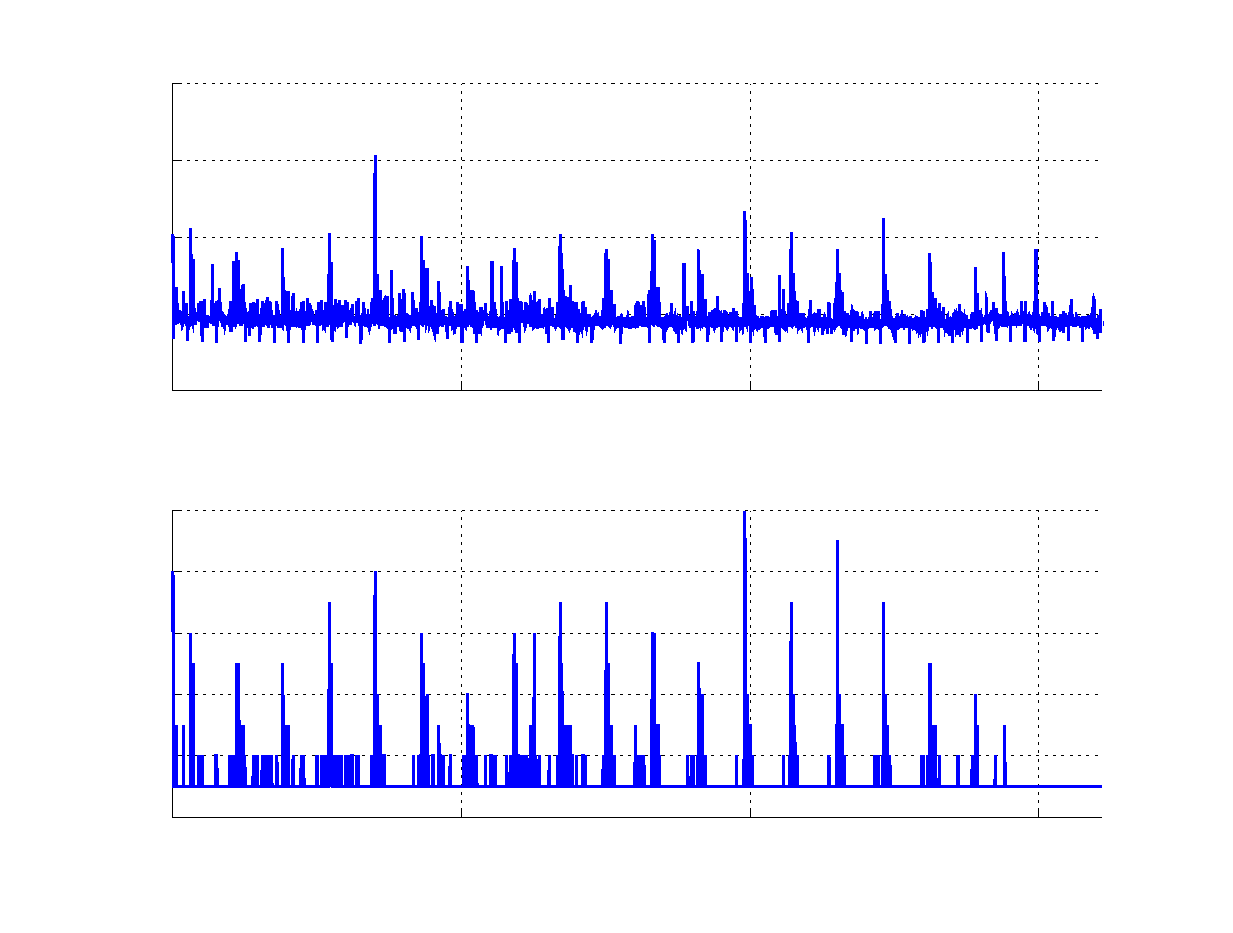
\includegraphics[trim=30  20   0   0,clip,scale=0.42]{time_16_02_04_N8_nodist-inc}
\end{picture}%
\begin{picture}(546, 412)(30,20)
\fontsize{8}{0}
\selectfont\put(74.88,247.205){\makebox(0,0)[t]{\textcolor[rgb]{0,0,0}{{0}}}}
\fontsize{8}{0}
\selectfont\put(213.47,247.205){\makebox(0,0)[t]{\textcolor[rgb]{0,0,0}{{5}}}}
\fontsize{8}{0}
\selectfont\put(352.061,247.205){\makebox(0,0)[t]{\textcolor[rgb]{0,0,0}{{10}}}}
\fontsize{8}{0}
\selectfont\put(490.651,247.205){\makebox(0,0)[t]{\textcolor[rgb]{0,0,0}{{15}}}}
\fontsize{8}{0}
\selectfont\put(69.8755,252.218){\makebox(0,0)[r]{\textcolor[rgb]{0,0,0}{{0}}}}
\fontsize{8}{0}
\selectfont\put(69.8755,289.063){\makebox(0,0)[r]{\textcolor[rgb]{0,0,0}{{1}}}}
\fontsize{8}{0}
\selectfont\put(69.8755,325.909){\makebox(0,0)[r]{\textcolor[rgb]{0,0,0}{{2}}}}
\fontsize{8}{0}
\selectfont\put(69.8755,362.754){\makebox(0,0)[r]{\textcolor[rgb]{0,0,0}{{3}}}}
\fontsize{8}{0}
\selectfont\put(69.8755,399.6){\makebox(0,0)[r]{\textcolor[rgb]{0,0,0}{{4}}}}
\fontsize{8}{0}
\selectfont\put(48.8755,325.909){\rotatebox{90}{\makebox(0,0)[b]{\textcolor[rgb]{0,0,0}{{comp. time $[ms]$}}}}}
\fontsize{8}{0}
\selectfont\put(74.88,42.507){\makebox(0,0)[t]{\textcolor[rgb]{0,0,0}{{0}}}}
\fontsize{8}{0}
\selectfont\put(213.47,42.507){\makebox(0,0)[t]{\textcolor[rgb]{0,0,0}{{5}}}}
\fontsize{8}{0}
\selectfont\put(352.061,42.507){\makebox(0,0)[t]{\textcolor[rgb]{0,0,0}{{10}}}}
\fontsize{8}{0}
\selectfont\put(490.651,42.507){\makebox(0,0)[t]{\textcolor[rgb]{0,0,0}{{15}}}}
\fontsize{8}{0}
\selectfont\put(69.8755,47.52){\makebox(0,0)[r]{\textcolor[rgb]{0,0,0}{{0}}}}
\fontsize{8}{0}
\selectfont\put(69.8755,76.9964){\makebox(0,0)[r]{\textcolor[rgb]{0,0,0}{{2}}}}
\fontsize{8}{0}
\selectfont\put(69.8755,106.473){\makebox(0,0)[r]{\textcolor[rgb]{0,0,0}{{4}}}}
\fontsize{8}{0}
\selectfont\put(69.8755,135.949){\makebox(0,0)[r]{\textcolor[rgb]{0,0,0}{{6}}}}
\fontsize{8}{0}
\selectfont\put(69.8755,165.426){\makebox(0,0)[r]{\textcolor[rgb]{0,0,0}{{8}}}}
\fontsize{8}{0}
\selectfont\put(69.8755,194.902){\makebox(0,0)[r]{\textcolor[rgb]{0,0,0}{{10}}}}
\fontsize{8}{0}
\selectfont\put(298.08,9.50697){\makebox(0,0)[t]{\textcolor[rgb]{0,0,0}{{simulation time $[s]$}}}}
\fontsize{8}{0}
\selectfont\put(31.8755,121.211){\rotatebox{90}{\makebox(0,0)[t]{\textcolor[rgb]{0,0,0}{{num. of iterations}}}}}
\end{picture}

            \subcaption{
                $N = 8$, without disturbances.\\
                Mean computational time: $9.4~[\MT{ms}]$.\\
                Time measurements $> 1~[\MT{ms}]$: 11\%
            }
            \label{fig.task_walk_time.3}
        }
    \end{minipage}
    \hfill
    \begin{minipage}[t]{0.49\textwidth}
        \centering{
            % Title: glps_renderer figure
% Creator: GL2PS 1.3.8, (C) 1999-2012 C. Geuzaine
% For: Octave
% CreationDate: Wed Mar 23 19:36:50 2016
\setlength{\unitlength}{0.42pt}
\begin{picture}(0,0)
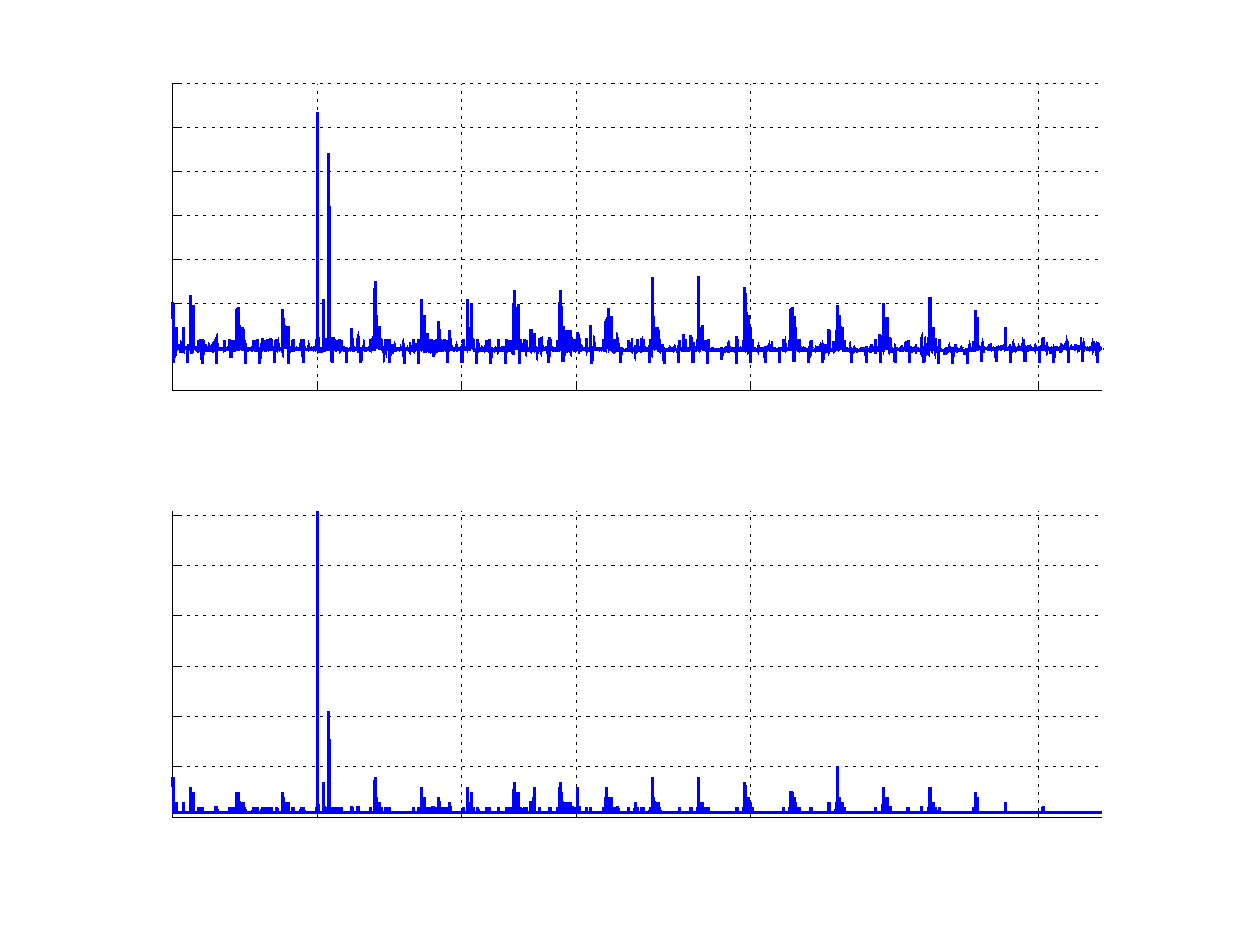
\includegraphics[trim=30  20   0   0,clip,scale=0.42]{time_16_02_02_N8-inc}
\end{picture}%
\begin{picture}(546, 412)(30,20)
\fontsize{8}{0}
\selectfont\put(74.88,247.205){\makebox(0,0)[t]{\textcolor[rgb]{0,0,0}{{0}}}}
\fontsize{8}{0}
\selectfont\put(144.175,247.205){\makebox(0,0)[t]{\textcolor[rgb]{0,0,0}{{$\impulseC_d^y$}}}}
\fontsize{8}{0}
\selectfont\put(213.47,247.205){\makebox(0,0)[t]{\textcolor[rgb]{0,0,0}{{5}}}}
\fontsize{8}{0}
\selectfont\put(268.907,247.205){\makebox(0,0)[t]{\textcolor[rgb]{0,0,0}{{$\impulseC_d^x$}}}}
\fontsize{8}{0}
\selectfont\put(352.061,247.205){\makebox(0,0)[t]{\textcolor[rgb]{0,0,0}{{10}}}}
\fontsize{8}{0}
\selectfont\put(490.651,247.205){\makebox(0,0)[t]{\textcolor[rgb]{0,0,0}{{15}}}}
\fontsize{8}{0}
\selectfont\put(69.8755,252.218){\makebox(0,0)[r]{\textcolor[rgb]{0,0,0}{{0}}}}
\fontsize{8}{0}
\selectfont\put(69.8755,273.272){\makebox(0,0)[r]{\textcolor[rgb]{0,0,0}{{1}}}}
\fontsize{8}{0}
\selectfont\put(69.8755,294.327){\makebox(0,0)[r]{\textcolor[rgb]{0,0,0}{{2}}}}
\fontsize{8}{0}
\selectfont\put(69.8755,315.382){\makebox(0,0)[r]{\textcolor[rgb]{0,0,0}{{3}}}}
\fontsize{8}{0}
\selectfont\put(69.8755,336.436){\makebox(0,0)[r]{\textcolor[rgb]{0,0,0}{{4}}}}
\fontsize{8}{0}
\selectfont\put(69.8755,357.491){\makebox(0,0)[r]{\textcolor[rgb]{0,0,0}{{5}}}}
\fontsize{8}{0}
\selectfont\put(69.8755,378.545){\makebox(0,0)[r]{\textcolor[rgb]{0,0,0}{{6}}}}
\fontsize{8}{0}
\selectfont\put(69.8755,399.6){\makebox(0,0)[r]{\textcolor[rgb]{0,0,0}{{7}}}}
\fontsize{8}{0}
\selectfont\put(48.8755,325.909){\rotatebox{90}{\makebox(0,0)[b]{\textcolor[rgb]{0,0,0}{{comp. time $[ms]$}}}}}
\fontsize{8}{0}
\selectfont\put(74.88,42.507){\makebox(0,0)[t]{\textcolor[rgb]{0,0,0}{{0}}}}
\fontsize{8}{0}
\selectfont\put(144.175,42.507){\makebox(0,0)[t]{\textcolor[rgb]{0,0,0}{{$\impulseC_d^y$}}}}
\fontsize{8}{0}
\selectfont\put(213.47,42.507){\makebox(0,0)[t]{\textcolor[rgb]{0,0,0}{{5}}}}
\fontsize{8}{0}
\selectfont\put(268.907,42.507){\makebox(0,0)[t]{\textcolor[rgb]{0,0,0}{{$\impulseC_d^x$}}}}
\fontsize{8}{0}
\selectfont\put(352.061,42.507){\makebox(0,0)[t]{\textcolor[rgb]{0,0,0}{{10}}}}
\fontsize{8}{0}
\selectfont\put(490.651,42.507){\makebox(0,0)[t]{\textcolor[rgb]{0,0,0}{{15}}}}
\fontsize{8}{0}
\selectfont\put(69.8755,47.52){\makebox(0,0)[r]{\textcolor[rgb]{0,0,0}{{0}}}}
\fontsize{8}{0}
\selectfont\put(69.8755,71.681){\makebox(0,0)[r]{\textcolor[rgb]{0,0,0}{{10}}}}
\fontsize{8}{0}
\selectfont\put(69.8755,95.842){\makebox(0,0)[r]{\textcolor[rgb]{0,0,0}{{20}}}}
\fontsize{8}{0}
\selectfont\put(69.8755,120.003){\makebox(0,0)[r]{\textcolor[rgb]{0,0,0}{{30}}}}
\fontsize{8}{0}
\selectfont\put(69.8755,144.164){\makebox(0,0)[r]{\textcolor[rgb]{0,0,0}{{40}}}}
\fontsize{8}{0}
\selectfont\put(69.8755,168.325){\makebox(0,0)[r]{\textcolor[rgb]{0,0,0}{{50}}}}
\fontsize{8}{0}
\selectfont\put(69.8755,192.486){\makebox(0,0)[r]{\textcolor[rgb]{0,0,0}{{60}}}}
\fontsize{8}{0}
\selectfont\put(298.08,9.50697){\makebox(0,0)[t]{\textcolor[rgb]{0,0,0}{{simulation time $[s]$}}}}
\fontsize{8}{0}
\selectfont\put(31.8755,121.211){\rotatebox{90}{\makebox(0,0)[b]{\textcolor[rgb]{0,0,0}{{num. of iterations}}}}}
\end{picture}

            \subcaption{
                $N = 8$, with disturbances.\\
                Mean computational time: $9.8~[\MT{ms}]$.\\
                Time measurements $> 1~[\MT{ms}]$: 13\%
            }
            \label{fig.task_walk_time.4}
        }
    \end{minipage}
    \caption[Computation time and number of iterations of \sn{LexLS}.]{
        Computation time and number of iterations of \sn{LexLS}. Time instants,
        when disturbances are applied, are indicated with $\impulseC_d^y$ and
        $\impulseC_d^x$.
    }
    \label{fig.task_walk_time}
\end{figure*}


\cref{hr.mmpc_walk} is supposed to be solved in order of milliseconds to
control a robot in real time. This is a challenging problem, since the
hierarchy has around $85$ decision variables and includes more than $100$
inequality and $120$ equality constraints. In order to demonstrate that this is
possible we measured the time required for \sn{LexLS} to solve this \ac{PLLS}
problem (see \cref{fig.task_walk_time.1,fig.task_walk_time.2}). The time
measurement at each control instant is averaged over three simulation runs to
suppress outliers. All measurements were performed on a laptop with Intel Core
i5-3360M ($2.80~[\MT{GHz}]$) \acs{CPU}.


When disturbances are not applied, the time required to solve the hierarchy is
less than $5~[\MT{ms}]$, the number of iterations of the solver does not exceed
$8$. However, disturbances lead to increase in the number of iterations of the
solver, which, in turn, leads to significant increase in the computational
time. In order to alleviate this issue it might be necessary to employ early
termination of the solver (see \cref{sec.early_termination}). It is, however,
important to note, that the current implementation of \sn{LexLS} adds and
removes constraints from the active set in an inefficient way
\cite{Dimitrov2015preprint}. Hence, further development of the solver is
expected to give a performance boost for the controller. In an attempt to
reduce the computational time, we also tried to shorten the preview horizon
from $N = 16$ to $N = 8$ sampling intervals. This modification reduces the
number of decision variables by $16$-$18$, the number of equality and
inequality constraints by $32$ and $16$-$18$ respectively. The problem with
shorter preview horizon can be solved slightly faster on average and 2 times
faster, when disturbance is applied (see
\cref{fig.task_walk_time.3,fig.task_walk_time.4}). One can also observe that in
almost $90$\% of the cases the problem is solved faster than $1~[\MT{ms}]$. At
the same time, we did not observe qualitative changes in behavior of the robot.



%%%%%%%%%%%%%%%%%%%%%%%%%%%%%%%%%%%%%%%%%%%%%%%%%%%%%%%%%%%%%%%%%%%%%%%%%%%%%%%%
\subsubsection{Quality of the motion}\label{sec.motion_quality}

Although, the controller produces the desired behavior, the generated motion is
not completely satisfactory:
%
\begin{itemize}
    \item \cref{fig.task_walk_x,fig.task_walk_y} demonstrate that the right
        hand position oscillates near the target in the end of the simulation
        due to the sway motion of the robot. This may be caused by several
        reasons: ({\bf i}) compromise between satisfaction of the hand task and
        other tasks on the last level of the hierarchy, ({\bf ii}) lack of
        anticipation for the hand position and respective kinematic
        constraints.

    \item We can see in \cref{fig.task_walk_steps_time_x_magnified} (as well as
        in \cref{fig.task_walk_steps_time_x,fig.task_walk_steps_time_y})
        periodic variations of the \ac{CoP} position with period of
        $0.1~[\MT{s}]$ caused by the discrepancy between the control interval
        of $0.005~[\MT{s}]$ and preview sampling interval of $0.1~[\MT{s}]$.
        This issue was discussed in \cref{sec.sampling_interval}.

\begin{figure}[!htbp]
    \centering{
        % Title: glps_renderer figure
% Creator: GL2PS 1.3.8, (C) 1999-2012 C. Geuzaine
% For: Octave
% CreationDate: Wed Mar 30 19:27:51 2016
\setlength{\unitlength}{0.7pt}
\begin{picture}(0,0)
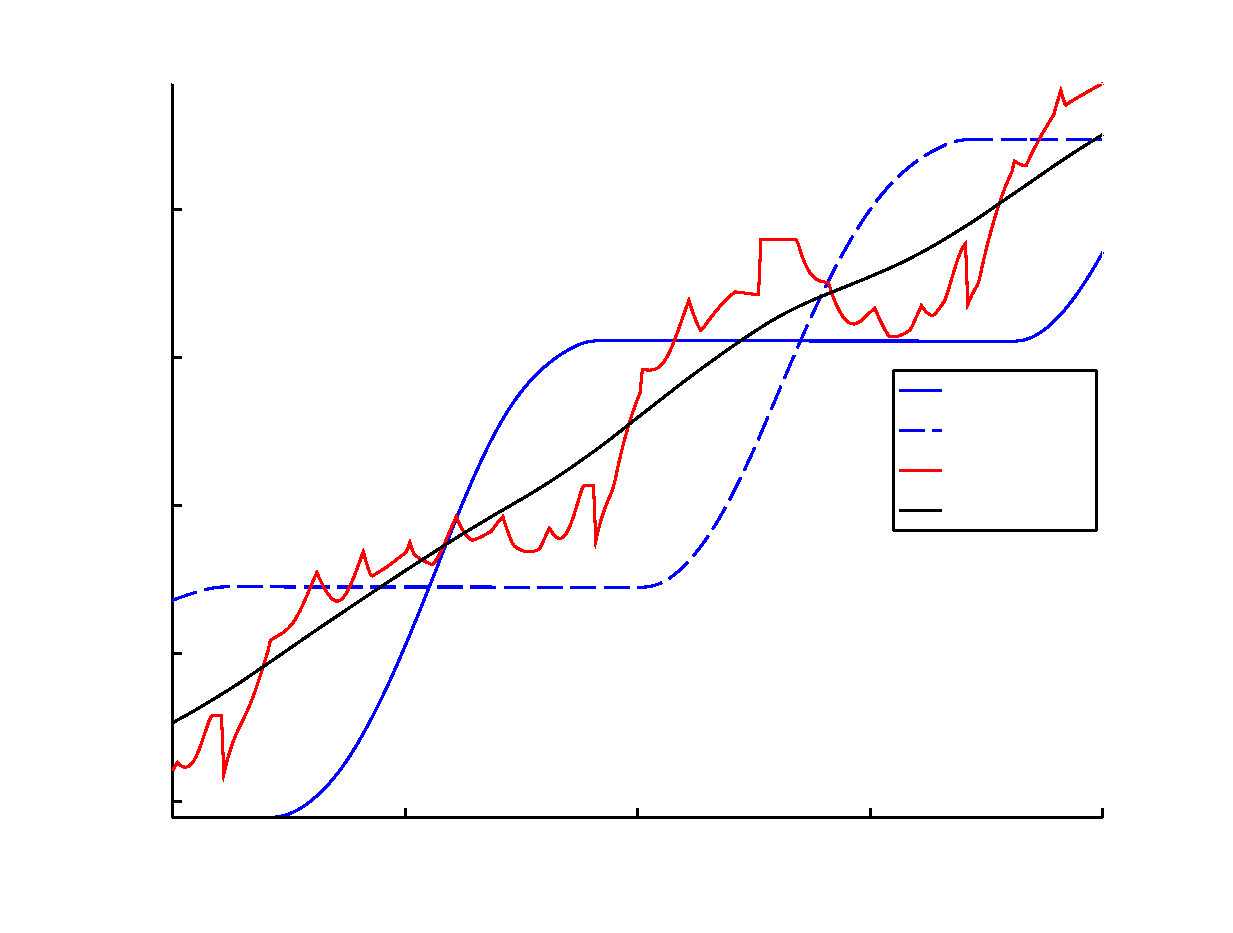
\includegraphics[trim=50   0  50  10,clip,scale=0.7]{steps_time_x_16_02_01_N16_nodist_magnified-inc}
\end{picture}%
\begin{picture}(476, 422)(50,0)
\fontsize{11}{0}
\selectfont\put(74.88,42.5188){\makebox(0,0)[t]{\textcolor[rgb]{0,0,0}{{5}}}}
\fontsize{11}{0}
\selectfont\put(186.48,42.5188){\makebox(0,0)[t]{\textcolor[rgb]{0,0,0}{{5.5}}}}
\fontsize{11}{0}
\selectfont\put(298.08,42.5188){\makebox(0,0)[t]{\textcolor[rgb]{0,0,0}{{6}}}}
\fontsize{11}{0}
\selectfont\put(409.68,42.5188){\makebox(0,0)[t]{\textcolor[rgb]{0,0,0}{{6.5}}}}
\fontsize{11}{0}
\selectfont\put(521.28,42.5188){\makebox(0,0)[t]{\textcolor[rgb]{0,0,0}{{7}}}}
\fontsize{11}{0}
\selectfont\put(69.8755,54.9812){\makebox(0,0)[r]{\textcolor[rgb]{0,0,0}{{0.6}}}}
\fontsize{11}{0}
\selectfont\put(69.8755,126.071){\makebox(0,0)[r]{\textcolor[rgb]{0,0,0}{{0.7}}}}
\fontsize{11}{0}
\selectfont\put(69.8755,197.161){\makebox(0,0)[r]{\textcolor[rgb]{0,0,0}{{0.8}}}}
\fontsize{11}{0}
\selectfont\put(69.8755,268.25){\makebox(0,0)[r]{\textcolor[rgb]{0,0,0}{{0.9}}}}
\fontsize{11}{0}
\selectfont\put(69.8755,339.34){\makebox(0,0)[r]{\textcolor[rgb]{0,0,0}{{1}}}}
\fontsize{11}{0}
\selectfont\put(298.08,22.5188){\makebox(0,0)[t]{\textcolor[rgb]{0,0,0}{{simulation time $[s]$}}}}
\fontsize{11}{0}
\selectfont\put(40.8755,223.56){\rotatebox{90}{\makebox(0,0)[b]{\textcolor[rgb]{0,0,0}{{position along the $x$ axis $[m]$}}}}}
\fontsize{11}{0}
\selectfont\put(446.874,252.364){\makebox(0,0)[l]{\textcolor[rgb]{0,0,0}{{Left foot}}}}
\fontsize{11}{0}
\selectfont\put(446.874,233.161){\makebox(0,0)[l]{\textcolor[rgb]{0,0,0}{{Right foot}}}}
\fontsize{11}{0}
\selectfont\put(446.874,213.959){\makebox(0,0)[l]{\textcolor[rgb]{0,0,0}{{CoP}}}}
\fontsize{11}{0}
\selectfont\put(446.874,194.756){\makebox(0,0)[l]{\textcolor[rgb]{0,0,0}{{CoM}}}}
\end{picture}

        \caption[Periodic variations in the CoP position.]{
            Magnified part of \cref{fig.task_walk_steps_time_x.nodist}:
            evolution of the feet, \ac{CoM}, and \ac{CoP} positions with time
            along the $x$ axis. Periodic variations of the \ac{CoP} position
            with period $0.1~[\MT{s}]$ can be clearly seen.
        }
        \label{fig.task_walk_steps_time_x_magnified}
    }
\end{figure}

    \item The controller is designed in such a way, that it always trades off
        between two strategies for reaching the target: moving the hand and
        walking. Consequently, near singularities of the elbow, the controller
        prefers walking to bending the arm, which is undesirable in some
        situations.

    \item We tuned the weights on the last level of the hierarchy so that the
        \ac{CoP} centering task dominates all others. The reason for this is
        that the hand task ``pulls'' the \ac{CoP} to the front edges of the
        support areas, which, to some extend, corresponds to walking on
        tiptoes. This negatively impacts controller's ability to cope with
        disturbances and, therefore, is potentially unsafe
        \cite{Lafaye2014humanoids}. Moreover, it leads to a larger number of
        active inequality constraints and larger number of iterations of the
        solver.
\end{itemize}



%%%%%%%%%%%%%%%%%%%%%%%%%%%%%%%%%%%%%%%%%%%%%%%%%%%%%%%%%%%%%%%%%%%%%%%%%%%%%%%%
\subsection{Conclusion}\label{sec.task_walk_conclusion}

We demonstrated that \ac{MMPC} allows to account for the whole body tasks while
generating walking motions without relying on time-demanding planning and
nonlinear optimization procedures \cite{Escande2009iros, Kanoun2010ijrr,
Tassa2014icra}. The major limitation of the approach is the fact that durations
and sequence of the steps must still be decided outside of the controller.
There is also a number of technical difficulties discussed in
\cref{sec.motion_quality}, which should be addressed in the future works.


\FloatBarrier



%%%%%%%%%%%%%%%%%%%%%%%%%%%%%%%%%%%%%%%%%%%%%%%%%%%%%%%%%%%%%%%%%%%%%%%%%%%%%%%%
%%%%%%%%%%%%%%%%%%%%%%%%%%%%%%%%%%%%%%%%%%%%%%%%%%%%%%%%%%%%%%%%%%%%%%%%%%%%%%%%
%%%%%%%%%%%%%%%%%%%%%%%%%%%%%%%%%%%%%%%%%%%%%%%%%%%%%%%%%%%%%%%%%%%%%%%%%%%%%%%%
\section{Prioritization in the contact force distribution}\label{sec.optional_force}

We continued to develop the idea of \ac{MMPC} in \cite{Sherikov2015humanoids},
where we proposed a controller for balancing in a multicontact setting with
prioritized contact force distribution. In most settings with multiple contacts
there exists an infinite number of force distributions that achieve the same
base motion. The typical approach to resolve this ambiguity is to make contacts
as robust as possible, by keeping each contact force far from the bounds of the
respective friction cone, and distribute the forces evenly between all the
contacts~\cite{Saab2013tro, Ott2011humanoids, Herzog2015auro, Hyon2007tro}.
There are situations, however, such as when a contact area is fragile, when it
is preferable to avoid using it unless strictly necessary for balance. In this
case, distributing forces evenly between all possible contacts should be
avoided. We propose therefore to introduce a prioritized distribution of the
contact forces, with the help of hierarchical optimization~\cite{Saab2013tro,
Escande2014ijrr, Kanoun2011tro}. We demonstrate our idea in a setting, where a
humanoid robot can optionally exploit a hand contact with an additional support
to maintain balance and execute certain task with the free hand.



%%%%%%%%%%%%%%%%%%%%%%%%%%%%%%%%%%%%%%%%%%%%%%%%%%%%%%%%%%%%%%%%%%%%%%%%%%%%%%%%
\subsection{Setting}\label{sec.force_setting}

\begin{figure}[!htb]
    \begin{minipage}[t]{0.49\textwidth}
        \centering{
            % Title: glps_renderer figure
% Creator: GL2PS 1.3.8, (C) 1999-2012 C. Geuzaine
% For: Octave
% CreationDate: Mon May  9 19:27:08 2016
\setlength{\unitlength}{0.42pt}
\begin{picture}(0,0)
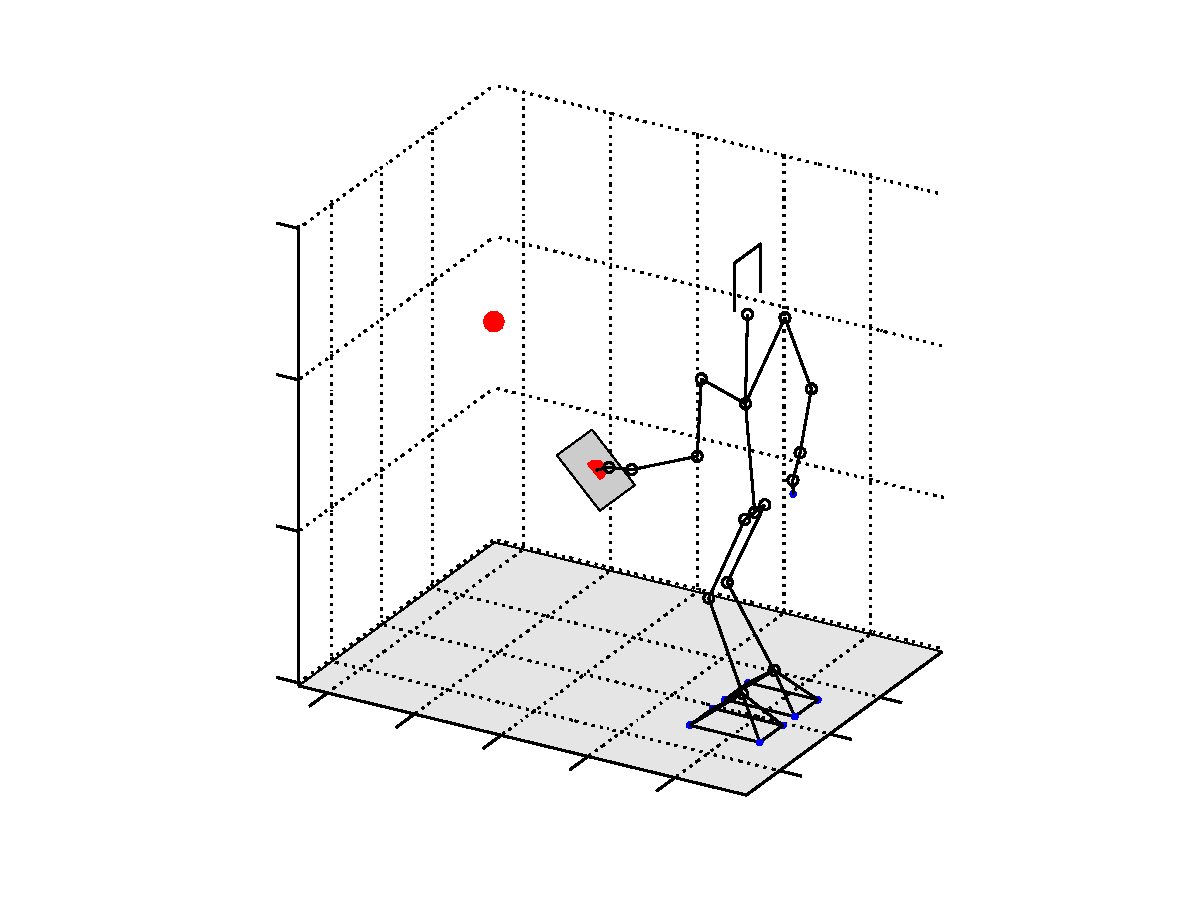
\includegraphics[trim=50  46  50   0,clip,scale=0.42]{test_17_23_robot_1-inc}
\end{picture}%
\begin{picture}(460, 374)(50,46)
\fontsize{7}{0}
\selectfont\put(119.905,103.852){\makebox(0,0)[br]{\textcolor[rgb]{0,0,0}{{0}}}}
\fontsize{7}{0}
\selectfont\put(119.905,176.551){\makebox(0,0)[br]{\textcolor[rgb]{0,0,0}{{0.5}}}}
\fontsize{7}{0}
\selectfont\put(119.905,249.249){\makebox(0,0)[br]{\textcolor[rgb]{0,0,0}{{1}}}}
\fontsize{7}{0}
\selectfont\put(119.905,321.947){\makebox(0,0)[br]{\textcolor[rgb]{0,0,0}{{1.5}}}}
\fontsize{7}{0}
\selectfont\put(429.718,89.3565){\makebox(0,0)[tl]{\textcolor[rgb]{0,0,0}{{-0.3}}}}
\fontsize{7}{0}
\selectfont\put(136.413,85.8912){\makebox(0,0)[tr]{\textcolor[rgb]{0,0,0}{{1.2}}}}
\fontsize{7}{0}
\selectfont\put(178.093,75.7213){\makebox(0,0)[tr]{\textcolor[rgb]{0,0,0}{{0.9}}}}
\fontsize{7}{0}
\selectfont\put(405.654,71.7417){\makebox(0,0)[tl]{\textcolor[rgb]{0,0,0}{{0}}}}
\fontsize{7}{0}
\selectfont\put(219.773,65.5514){\makebox(0,0)[tr]{\textcolor[rgb]{0,0,0}{{0.6}}}}
\fontsize{7}{0}
\selectfont\put(261.453,55.3814){\makebox(0,0)[tr]{\textcolor[rgb]{0,0,0}{{0.3}}}}
\fontsize{7}{0}
\selectfont\put(303.133,45.2115){\makebox(0,0)[tr]{\textcolor[rgb]{0,0,0}{{0}}}}
\fontsize{7}{0}
\selectfont\put(381.59,54.1268){\makebox(0,0)[tl]{\textcolor[rgb]{0,0,0}{{0.3}}}}
\end{picture}

            \subcaption{initial configuration}
            \label{fig.force_distrib.1}
        }
    \end{minipage}
    \hfill
    \begin{minipage}[t]{0.49\textwidth}
        \centering{
            \input{test_17_23_robot_1001.tex}
            \subcaption{after $5$ seconds}
            \label{fig.force_distrib.2}
        }
    \end{minipage}
    \begin{minipage}[t]{0.49\textwidth}
        \centering{
            % Title: glps_renderer figure
% Creator: GL2PS 1.3.8, (C) 1999-2012 C. Geuzaine
% For: Octave
% CreationDate: Mon May  9 19:27:11 2016
\setlength{\unitlength}{0.42pt}
\begin{picture}(0,0)
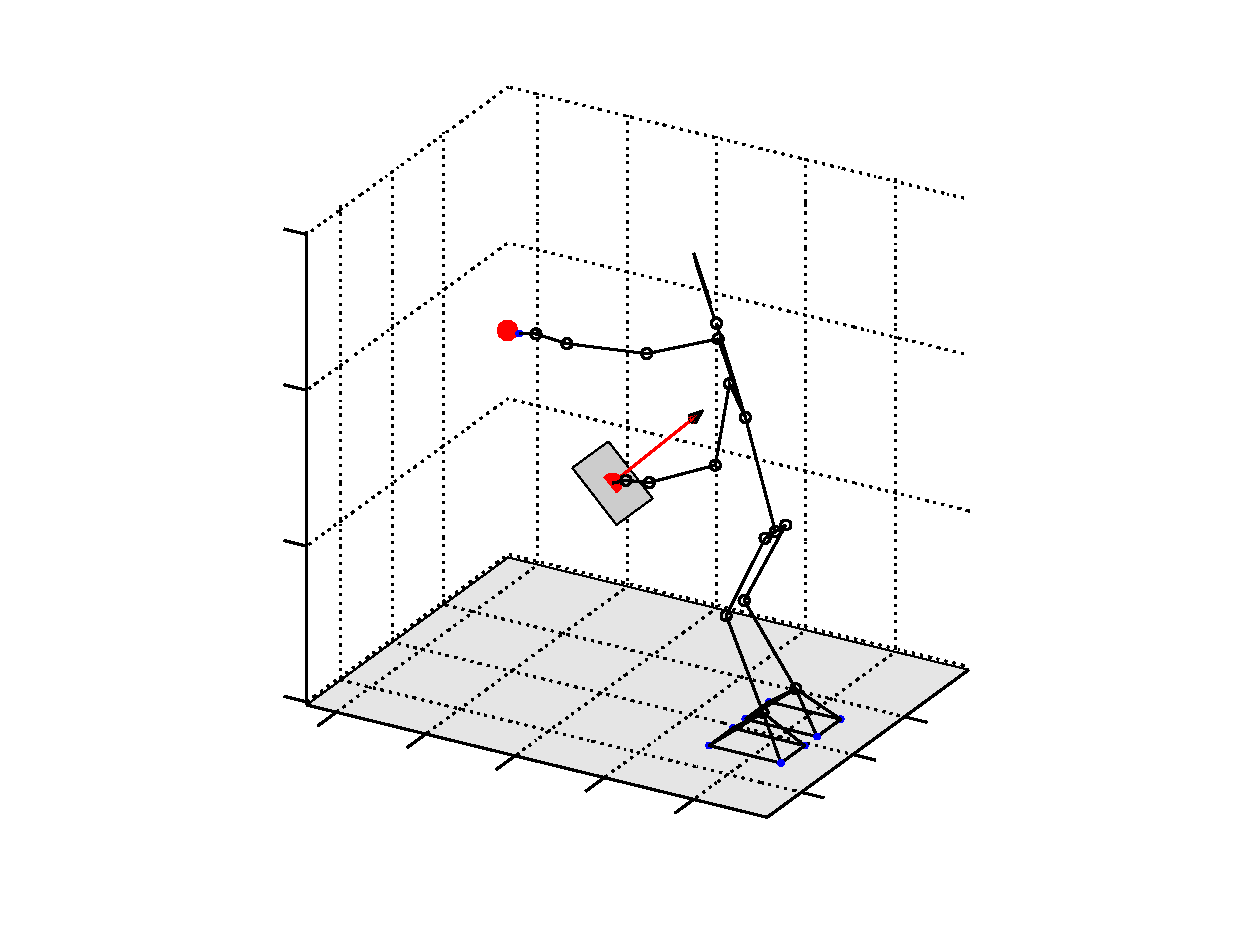
\includegraphics[trim=50  46  50   0,clip,scale=0.42]{test_17_23_robot_2001-inc}
\end{picture}%
\begin{picture}(476, 386)(50,46)
\fontsize{7}{0}
\selectfont\put(123.469,106.786){\makebox(0,0)[br]{\textcolor[rgb]{0,0,0}{{0}}}}
\fontsize{7}{0}
\selectfont\put(123.469,181.561){\makebox(0,0)[br]{\textcolor[rgb]{0,0,0}{{0.5}}}}
\fontsize{7}{0}
\selectfont\put(123.469,256.337){\makebox(0,0)[br]{\textcolor[rgb]{0,0,0}{{1}}}}
\fontsize{7}{0}
\selectfont\put(123.469,331.112){\makebox(0,0)[br]{\textcolor[rgb]{0,0,0}{{1.5}}}}
\fontsize{7}{0}
\selectfont\put(140.455,88.4511){\makebox(0,0)[tr]{\textcolor[rgb]{0,0,0}{{1.2}}}}
\fontsize{7}{0}
\selectfont\put(183.326,77.9906){\makebox(0,0)[tr]{\textcolor[rgb]{0,0,0}{{0.9}}}}
\fontsize{7}{0}
\selectfont\put(226.197,67.5301){\makebox(0,0)[tr]{\textcolor[rgb]{0,0,0}{{0.6}}}}
\fontsize{7}{0}
\selectfont\put(269.068,57.0696){\makebox(0,0)[tr]{\textcolor[rgb]{0,0,0}{{0.3}}}}
\fontsize{7}{0}
\selectfont\put(311.939,46.6091){\makebox(0,0)[tr]{\textcolor[rgb]{0,0,0}{{0}}}}
\fontsize{7}{0}
\selectfont\put(441.858,91.9431){\makebox(0,0)[tl]{\textcolor[rgb]{0,0,0}{{-0.3}}}}
\fontsize{7}{0}
\selectfont\put(417.107,73.825){\makebox(0,0)[tl]{\textcolor[rgb]{0,0,0}{{0}}}}
\fontsize{7}{0}
\selectfont\put(392.355,55.7069){\makebox(0,0)[tl]{\textcolor[rgb]{0,0,0}{{0.3}}}}
\end{picture}

            \subcaption{after $10$ seconds}
            \label{fig.force_distrib.3}
        }
    \end{minipage}
    \hfill
    \begin{minipage}[t]{0.49\textwidth}
        \centering{
            \input{test_17_23_robot_3001.tex}
            \subcaption{after $15$ seconds}
            \label{fig.force_distrib.4}
        }
    \end{minipage}
    \begin{minipage}[t]{0.49\textwidth}
        \centering{
            \input{test_17_23_robot_4001.tex}
            \subcaption{after $20$ seconds}
            \label{fig.force_distrib.5}
        }
    \end{minipage}
    \hfill
    \begin{minipage}[t]{0.49\textwidth}
        \centering{
            \input{test_17_23_robot_5000.tex}
            \subcaption{after $30$ seconds}
            \label{fig.force_distrib.6}
        }
    \end{minipage}
    \caption[Prioritization of the contact forces: reaching task.]{
        Configurations of the robot while it is trying to reach a target
        indicated by the red point. Grey areas represent contact surfaces.
        Length of the arrow indicates magnitude of the contact force applied by
        the left hand.
    }
    \label{fig.force_distrib}
\end{figure}


We use the following setting: the robot is standing with its left hand
positioned on an additional support, while the right hand executes certain
task. Hence, the number of contacts $M = 3$ (two feet and the hand) is constant
during the simulations. We define two different hand tasks. In the first case
the robot has to reach a target, which is initially unreachable without using
the additional support and later moved closer to the robot (see
\cref{fig.force_distrib,fig.force_distrib_right_hand}). The second task is to
maintain position of the right hand while an external disturbing force is
acting on it (see \cref{fig.force_distrib_weight}). In other words, the robot
holds a heavy object, such as a filled bucket \cite{Stephens2010iros}. The
external force is varying with time and is assumed to be measured. In all tests
the controller is expected to apply a force on the additional support only if
necessary to preserve balance and execute the hand task.


\begin{figure}[!htbp]
    \centering{
        % Title: glps_renderer figure
% Creator: GL2PS 1.3.8, (C) 1999-2012 C. Geuzaine
% For: Octave
% CreationDate: Mon May  9 19:44:30 2016
\setlength{\unitlength}{0.5pt}
\begin{picture}(0,0)
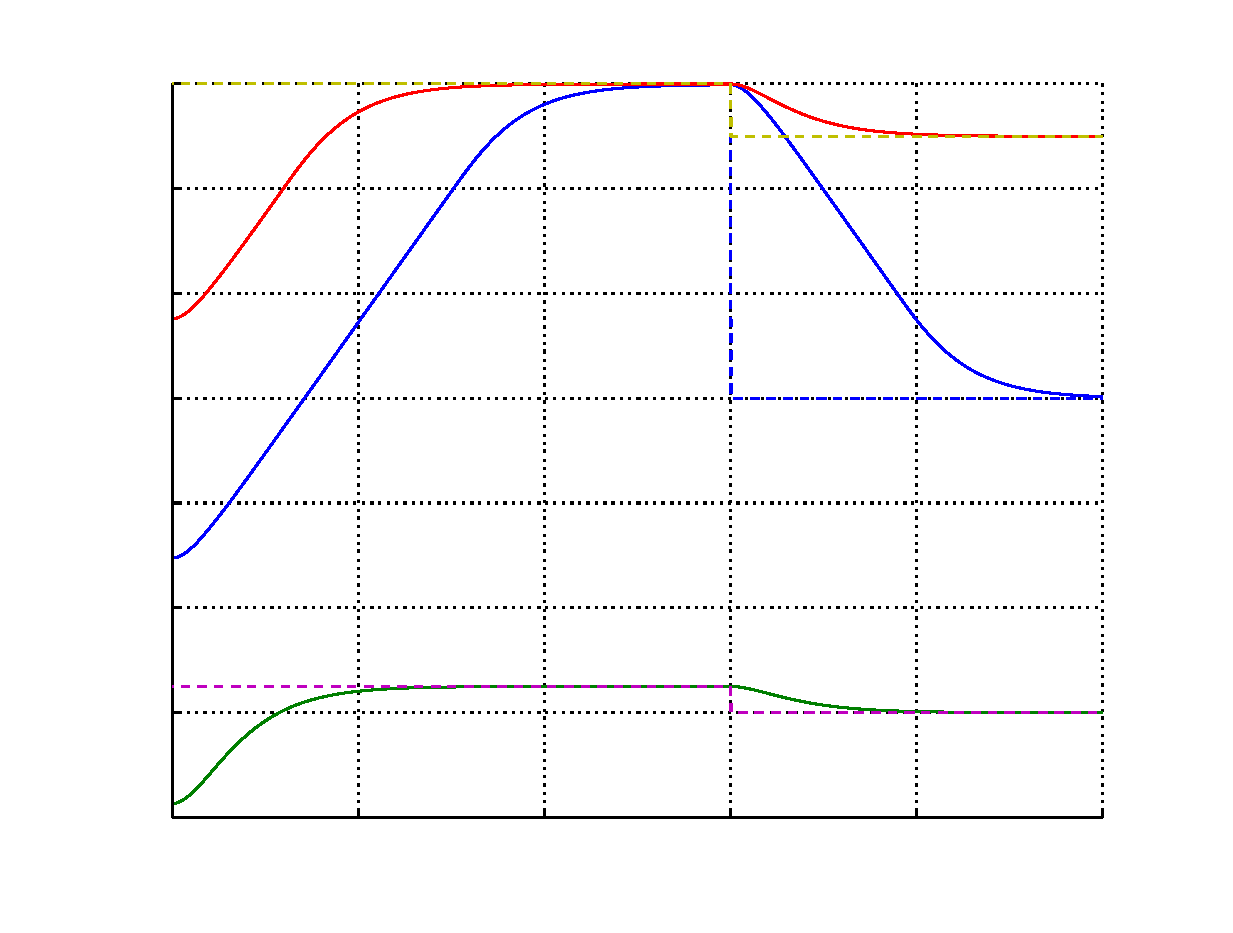
\includegraphics[trim=0  0  0  0,clip,scale=0.5]{test_17_23_position-inc}
\end{picture}%
\begin{picture}(576, 432)(0,0)
\fontsize{11}{0}
\selectfont\put(74.88,42.5189){\makebox(0,0)[t]{\textcolor[rgb]{0,0,0}{{0}}}}
\fontsize{11}{0}
\selectfont\put(164.16,42.5189){\makebox(0,0)[t]{\textcolor[rgb]{0,0,0}{{5}}}}
\fontsize{11}{0}
\selectfont\put(253.44,42.5189){\makebox(0,0)[t]{\textcolor[rgb]{0,0,0}{{10}}}}
\fontsize{11}{0}
\selectfont\put(342.72,42.5189){\makebox(0,0)[t]{\textcolor[rgb]{0,0,0}{{15}}}}
\fontsize{11}{0}
\selectfont\put(432,42.5189){\makebox(0,0)[t]{\textcolor[rgb]{0,0,0}{{20}}}}
\fontsize{11}{0}
\selectfont\put(521.28,42.5189){\makebox(0,0)[t]{\textcolor[rgb]{0,0,0}{{25}}}}
\fontsize{11}{0}
\selectfont\put(69.8755,47.52){\makebox(0,0)[r]{\textcolor[rgb]{0,0,0}{{-0.4}}}}
\fontsize{11}{0}
\selectfont\put(69.8755,97.8171){\makebox(0,0)[r]{\textcolor[rgb]{0,0,0}{{-0.2}}}}
\fontsize{11}{0}
\selectfont\put(69.8755,148.114){\makebox(0,0)[r]{\textcolor[rgb]{0,0,0}{{0}}}}
\fontsize{11}{0}
\selectfont\put(69.8755,198.411){\makebox(0,0)[r]{\textcolor[rgb]{0,0,0}{{0.2}}}}
\fontsize{11}{0}
\selectfont\put(69.8755,248.709){\makebox(0,0)[r]{\textcolor[rgb]{0,0,0}{{0.4}}}}
\fontsize{11}{0}
\selectfont\put(69.8755,299.006){\makebox(0,0)[r]{\textcolor[rgb]{0,0,0}{{0.6}}}}
\fontsize{11}{0}
\selectfont\put(69.8755,349.303){\makebox(0,0)[r]{\textcolor[rgb]{0,0,0}{{0.8}}}}
\fontsize{11}{0}
\selectfont\put(69.8755,399.6){\makebox(0,0)[r]{\textcolor[rgb]{0,0,0}{{1}}}}
\fontsize{11}{0}
\selectfont\put(298.08,26.5189){\makebox(0,0)[t]{\textcolor[rgb]{0,0,0}{{simulation time $[s]$}}}}
\fontsize{11}{0}
\selectfont\put(40.8755,223.56){\rotatebox{90}{\makebox(0,0)[b]{\textcolor[rgb]{0,0,0}{{right hand position $[m]$}}}}}
\end{picture}

        \caption[Execution of the reaching right hand task.]{
            Position of the right hand during execution of the reaching task.
            $x$, $y$, and $z$ coordinates are shown in solid blue, green, and
            red respectively. The desired positions are shown in dashed lines.
        }
        \label{fig.force_distrib_right_hand}
    }
\end{figure}


\begin{figure}[!htbp]
    \begin{minipage}[t]{0.49\textwidth}
        \centering{
            \input{test_17_24_robot_1.tex}
            \subcaption{initial configuration}
            \label{fig.force_distrib_weight.1}
        }
    \end{minipage}
    \hfill
    \begin{minipage}[t]{0.49\textwidth}
        \centering{
            \input{test_17_24_robot_401.tex}
            \subcaption{after $2$ seconds}
            \label{fig.force_distrib_weight.2}
        }
    \end{minipage}
    \begin{minipage}[t]{0.49\textwidth}
        \centering{
            \input{test_17_24_robot_1001.tex}
            \subcaption{after $5$ seconds}
            \label{fig.force_distrib_weight.3}
        }
    \end{minipage}
    \hfill
    \begin{minipage}[t]{0.49\textwidth}
        \centering{
            % Title: glps_renderer figure
% Creator: GL2PS 1.3.8, (C) 1999-2012 C. Geuzaine
% For: Octave
% CreationDate: Fri Mar 18 18:16:07 2016
\setlength{\unitlength}{0.42pt}
\begin{picture}(0,0)
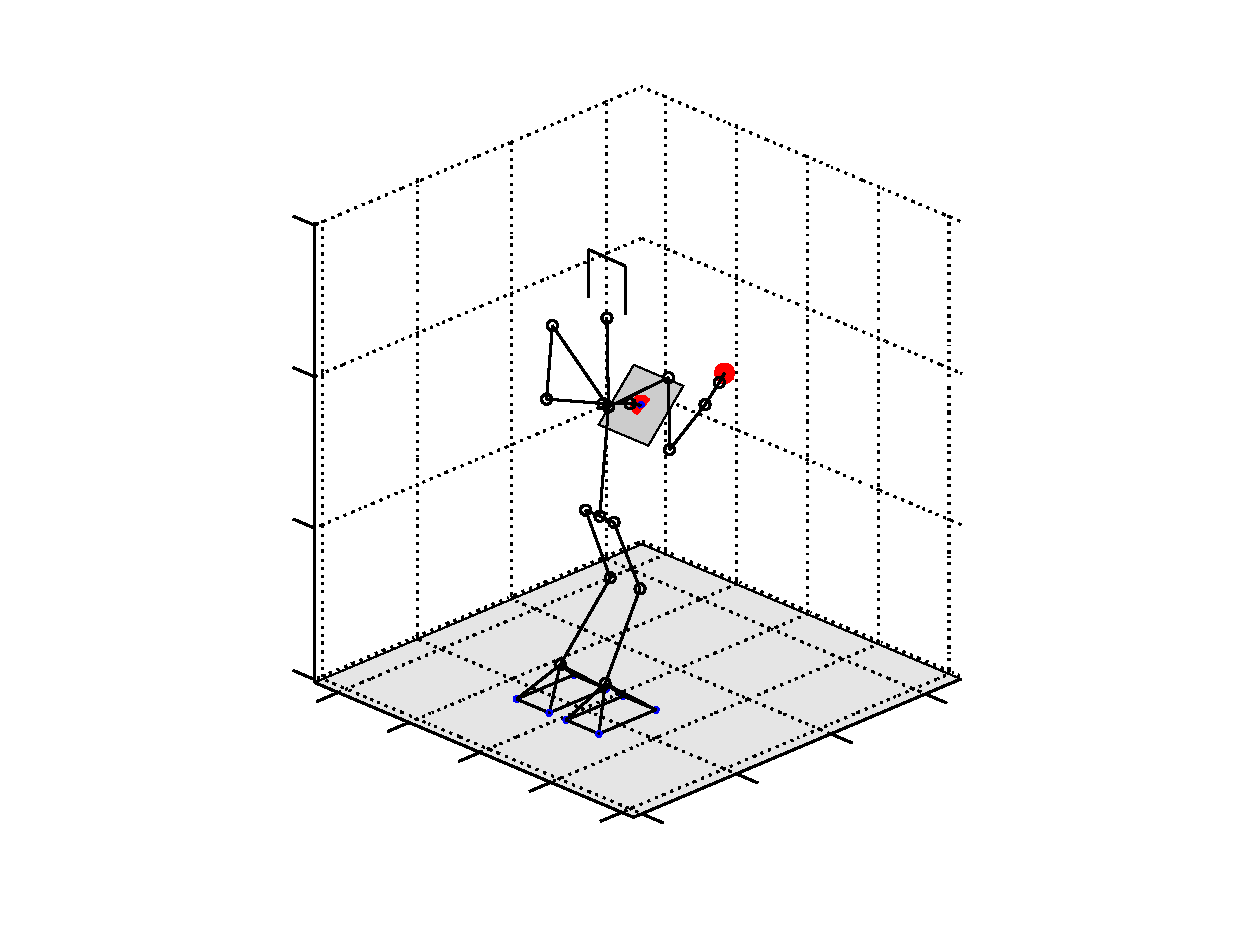
\includegraphics[trim=50  40  50  15,clip,scale=0.42]{test_17_24_robot_2000-inc}
\end{picture}%
\begin{picture}(476, 377)(50,40)
\fontsize{8}{0}
\selectfont\put(128.078,119.977){\makebox(0,0)[br]{\textcolor[rgb]{0,0,0}{{0}}}}
\fontsize{8}{0}
\selectfont\put(128.078,192.665){\makebox(0,0)[br]{\textcolor[rgb]{0,0,0}{{0.5}}}}
\fontsize{8}{0}
\selectfont\put(128.078,265.352){\makebox(0,0)[br]{\textcolor[rgb]{0,0,0}{{1}}}}
\fontsize{8}{0}
\selectfont\put(128.078,338.039){\makebox(0,0)[br]{\textcolor[rgb]{0,0,0}{{1.5}}}}
\fontsize{8}{0}
\selectfont\put(451.064,100.435){\makebox(0,0)[tl]{\textcolor[rgb]{0,0,0}{{0.8}}}}
\fontsize{8}{0}
\selectfont\put(139.398,101.139){\makebox(0,0)[tr]{\textcolor[rgb]{0,0,0}{{0.6}}}}
\fontsize{8}{0}
\selectfont\put(173.424,86.7588){\makebox(0,0)[tr]{\textcolor[rgb]{0,0,0}{{0.3}}}}
\fontsize{8}{0}
\selectfont\put(207.451,72.3785){\makebox(0,0)[tr]{\textcolor[rgb]{0,0,0}{{0}}}}
\fontsize{8}{0}
\selectfont\put(241.478,57.9982){\makebox(0,0)[tr]{\textcolor[rgb]{0,0,0}{{-0.3}}}}
\fontsize{8}{0}
\selectfont\put(275.504,43.6179){\makebox(0,0)[tr]{\textcolor[rgb]{0,0,0}{{-0.6}}}}
\fontsize{8}{0}
\selectfont\put(314.957,42.9134){\makebox(0,0)[tl]{\textcolor[rgb]{0,0,0}{{-0.4}}}}
\fontsize{8}{0}
\selectfont\put(360.326,62.0872){\makebox(0,0)[tl]{\textcolor[rgb]{0,0,0}{{0}}}}
\fontsize{8}{0}
\selectfont\put(405.695,81.2609){\makebox(0,0)[tl]{\textcolor[rgb]{0,0,0}{{0.4}}}}
\end{picture}

            \subcaption{after $10$ seconds}
            \label{fig.force_distrib_weight.4}
        }
    \end{minipage}
    \caption[Prioritization of the contact forces: disturbing force.]{
        Configurations of the robot in presence of varying disturbing force
        $\V{f}_{\MT{rh}}$. Grey areas represent contact surfaces. Length of the
        arrow indicates magnitude of the external force.
    }
    \label{fig.force_distrib_weight}
\end{figure}

\FloatBarrier


%%%%%%%%%%%%%%%%%%%%%%%%%%%%%%%%%%%%%%%%%%%%%%%%%%%%%%%%%%%%%%%%%%%%%%%%%%%%%%%%
\subsection{Design of the controller}\label{sec.force_controller}

The point-mass model exploited in \cref{hr.mmpc_walk} is not suitable for
multicontact scenarios. For this reason, we adopt the momenta-based
(\nameref{model.MB}) model and couple it with the whole body
(\nameref{model.WB}) model through the current contact forces. In order to
achieve high computational performance we condense \nameref{model.MB} and
eliminate torques from \nameref{model.WB} in advance (see
\cref{sec.plls_preprocessing}). Once this is done, the controller is formulated
as follows
%
\changeHierarchyStyle{width=14.5cm,before=,after=\par}{\setlength{\itemsep}{5pt}}
\begin{hierarchy}[hr.mmpc_force]
    \level Simple bounds
            \begin{itemize}
                \item \makebox[5cm][l]{
                        $\displaystyle \ubar{\ddq}^{\prime}  \le  \ddqn  \le  \bar{\ddq}^{\prime}$
                    }
                    $30$ joint limits

                \item \makebox[5cm][l]{
                        $\displaystyle \V{\lambda}_{k,i} \ge \V{0}$
                    }
                    $3 N M$ constraints due to friction cones
            \end{itemize}

    \level Whole body tasks and coupling
            \begin{itemize}
                \item
                    $\displaystyle
                        \begin{bmatrix}
                            \M{H}_2\\
                            \M{H}_3\\
                        \end{bmatrix}
                        \ddq
                        +
                        \begin{bmatrix}
                            \V{h}_2\\
                            \V{h}_3
                        \end{bmatrix}
                        =
                        m
                        \begin{bmatrix}
                            \T{\Jcom[,2]}\\
                            \T{\Jcom[,3]}
                        \end{bmatrix}
                        \V{g}
                        +
                        \begin{bmatrix}
                            \T{\M{J}_{\TRAN,\MT{lh},2}}\\
                            \T{\M{J}_{\TRAN,\MT{lh},3}}
                        \end{bmatrix}
                        \M{V}_{0, \MT{lh}} \V{\lambda}_{0, \MT{lh}}
                        +
                        \sum_{i=1}^{M-1}
                            \begin{bmatrix}
                                \T{\M{J}_{i,2}}\\
                                \T{\M{J}_{i,3}}
                            \end{bmatrix}
                            \begin{bmatrix}
                                \M{V}_{0,i} \V{\lambda}_{0,i}\\
                                \moment_{0,i}
                            \end{bmatrix}
                    $\\[1mm]
                    \makebox[5cm][l]{} $6$ equalities due to Newton-Euler equations

                \item
                    $\displaystyle
                    \ubar{\torques}
                    \le
                    \M{H}_1 \ddq  +  \V{h}_1  -  m \T{\Jcom[,1]} \V{g}
                    -
                    \T{\M{J}_{\TRAN,\MT{lh},1}}
                    \force_{\MT{lh},0}
                    -
                    \sum_{i=1}^{M-1}
                        \T{\M{J}_{i,1}}
                        \begin{bmatrix}
                            \M{V}_{0,i} \V{\lambda}_{0,i}\\
                            \moment_{0,i}
                        \end{bmatrix}
                    \le
                    \bar{\torques}
                    $\\[1mm]
                    \makebox[5cm][l]{} $30$ bounds on the joint torques

                \item
                    \makebox[5cm][l]{
                        $\displaystyle
                        \M{J}_i
                        \ddq
                        +
                        \dotM{J}_i
                        \dq
                        = \V{0}$
                    }
                    $6 M$ equalities due to fixed contacts
            \end{itemize}

           Anticipation tasks
            \begin{itemize}
                \item
                    \makebox[5cm][l]{
                        $\displaystyle
                        \sum_{i=1}^{M} \forceC_{k,i}^z
                        =
                        - m g^z$
                    }
                    $N$ equalities due to fixed \acs{CoM} height

                \item
                    \makebox[5cm][l]{
                        $\displaystyle
                        \objA_{\moment,k,i}
                        \begin{bmatrix}
                            \V{\lambda}_{k,i}\\
                            \moment_{k,i}
                        \end{bmatrix}
                        \ge
                        \ubarV{\objb}_{\moment,k,i}
                        $
                    }
                    $6 (M-1)$ constraints on the moments
            \end{itemize}

    \level Capturability constraint \cref{eq.capture_momenta_model}
            \begin{itemize}
                \item
                    \begin{minipage}[c]{5cm}
                        $\displaystyle
                        \V{\LM}^{xy}_N = \V{0},
                        \enspace \V[c]{\AM}^{xy}_N = \V{0},
                        $\\
                        $\displaystyle
                        \dotV{\LM}^{xy}_N = \V{0},
                        \enspace \dotV[c]{\AM}_N = \V{0}
                        $
                    \end{minipage}
                    $9$ equalities
            \end{itemize}

    \level Right hand task
            \begin{itemize}
                \item
                    \makebox[5cm][l]{
                        $\displaystyle
                        \M{J}_{\TRAN,\MT{rh}} \ddq + \dotM{J}_{\TRAN,\MT{rh}} \dq
                        =
                        \V{\pi}_{\MT{rh}}
                        $
                    }
                    $3$ equalities
            \end{itemize}

    \level Minimization of the normal left hand contact force
            \begin{itemize}
                \item
                    \makebox[5cm][l]{
                        $\displaystyle
                        \forceC_{k,\MT{lh}}^n = 0
                        $
                    }
                    $N$ equalities
            \end{itemize}

    \level Whole body tasks
            \begin{itemize}
                \item
                    \makebox[5.5cm][l]{
                        $\displaystyle
                        \M{L} \ddqn
                        =
                        \M{L}
                        \left(
                            \K_{p} (\qn[\DES] - \qn) - \K_{d} \dqn
                        \right)
                        $
                    }
                    $30$ equalities to control the joints
            \end{itemize}
           Anticipation tasks
            \begin{itemize}
                \item
                    \makebox[5cm][l]{
                        $\displaystyle
                        \V{\lambda}_{k,i} = \V{0}
                        $
                    }
                    $3 N M$ equalities to minimize forces

                \item
                    \makebox[5cm][l]{
                        $\displaystyle
                        \moment_{k,\{1,...,M-1\}} = \V{0}
                        $
                    }
                    $3 N (M-1)$ equalities to minimize moments
            \end{itemize}

    \vars{$\x = \left(\ddq, \V{\lambda}_{k,i}, \moment_{k,\{1,...,M-1\}}\right)$\\[1mm]
            \makebox[3.3cm]{} with $\quad i \in \{1, ..., M\}$, $\quad k \in \{0, ..., N-1\}$}%
\end{hierarchy}
\thesisHierarchyStyle{}%
%
where
%
\begin{longtable}[l]{@{\extracolsep{0pt}}l @{\extracolsep{1.5cm}}l}
    $\M{J}_{\MT{lh}} = (\M{J}_{\TRAN,\MT{lh}}, \M{J}_{\ROT,\MT{lh}})$   & Jacobian of the left hand,\\
    $\M{J}_{\TRAN,\MT{rh}}$                                             & translational Jacobian of the right hand,\\
    $\V{\pi}_{\MT{rh}}$                                                 & appropriately defined \acs{PD}-controller,\\
    $\M{L}$                                                             & Cholesky factor of $\M{H}$: $\T{\M{L}}\M{L} = \M{H}$.
\end{longtable}
%
\noindent Whenever the external force $\V{f}_{\MT{rh}}$ is applied to the right
hand, we account for its contribution in the equation of dynamics and joint
torque constraints.


The decision variables are
%
\begin{itemize}[topsep=0pt,parsep=0pt,itemsep=0pt]
    \item the generalized accelerations $\ddq$,
    \item current and anticipated contact forces represented with $\V{\lambda}_{k,i}$,
    \item current and anticipated contact moments $\moment_{k,\{1,...,M-1\}}$.
\end{itemize}
%
Note that the left hand contact moment with index $i = M$ is omitted, since
this contact is chosen to be a point contact. Final momenta and their rates
$\V{\LM}^{xy}_N$, $\V[c]{\AM}^{xy}_N$, $\dotV{\LM}^{xy}_N$, $\dotV[c]{\AM}_N$
are expressed through the decision variables $\x$ as explained in
\cref{sec.momenta_model_capturability}. The normal components of the optional
contact forces $\forceC_{k,\MT{lh}}^n$ are also expressed with
$\V{\lambda}_{k,\MT{lh}}$.


We achieve force prioritization using a separate priority level for
minimization of the optional contact force. This level is of lower priority
than the capturability constraints, which ensure the balance, and the right
hand task. At the same time, this level is more important than minimization of
all non-optional contact forces.


Length of the preview horizon is the same in all considered scenarios $N = 6$,
and the sampling interval of the preview horizon is set to $T_k = 0.1~[s]$.



%%%%%%%%%%%%%%%%%%%%%%%%%%%%%%%%%%%%%%%%%%%%%%%%%%%%%%%%%%%%%%%%%%%%%%%%%%%%%%%%%
\subsection{Results and discussion}\label{sec.force_results}

We observed that in both considered scenarios the controller produces the
desired behavior, \IE, it applies the hand contact force if necessary, and
stops applying it, when the need is gone (see
\cref{fig.force_distrib_task_force_com,fig.force_distrib_weight_force_com}).


Note that if the capturability constraint is omitted nothing prevents the
controller from sacrificing the balance in order to execute the hand task as
demonstrated in \cref{fig.force_distrib_task_force_com}. Contrary to the case
of the walking controller discussed in \cref{sec.task_walk}, the capturability
constraint appears to be sufficient for preservation of balance.


During construction and tuning of the controller one should keep in mind the
following aspects:
%
\begin{itemize}
    \item When the hand contact force minimization task starts to conflict with
        the higher priority objectives, the problem becomes singular. This
        results in violent accelerations of the joints illustrated in
        \cref{fig.chattering}. In order to avoid this we employ regularization
        of the \cref{hr.mmpc_force.4}-th and \cref{hr.mmpc_force.5}-th levels
        of the hierarchy using the objective on the final level as described in
        \cref{sec.regularization}. Due to lacking support of regularization in
        \sn{LexLS} we have to solve a sequence of \ac{PLLS} problems to obtain
        the solution (see \cref{app.regularization}).

    \item We have indicated earlier in \cref{sec.sampling_interval}, that the
        choice of sampling of the preview horizon may have a negative impact on
        the performance of the controller. This problem is illustrated in
        \cref{fig.subsampling}. Periodic variations in the norm of the hand
        contact force are produced by the controller, if we choose to reduce
        the first sampling interval by $5~[\MT{ms}]$ instead of shifting the
        whole preview horizon by $5~[\MT{ms}]$. These two approaches are
        discussed in detail in \cref{sec.sampling_interval}.
\end{itemize}
%

Though we have to solve the hierarchy in an inefficient way in order to
implement regularization as described in \cref{app.regularization}, the average
computation time is below $100~[\MT{ms}]$.


\begin{figure}[!htbp]
    \begin{minipage}[t]{\textwidth}
        \centering{
            \input{test_17_23_force.tex}
            \subcaption{
                Norms of the optional left hand contact forces. Force shown in
                solid blue line corresponds to the controller with the
                capturability constraint. The controller without the
                capturability constraint produces force shown in solid black.
            }
            \label{fig.force_distrib_task_force}
        }
    \end{minipage}
    \begin{minipage}[t]{\textwidth}
        \centering{
            % Title: glps_renderer figure
% Creator: GL2PS 1.3.8, (C) 1999-2012 C. Geuzaine
% For: Octave
% CreationDate: Mon May  9 19:44:29 2016
\setlength{\unitlength}{0.6pt}
\begin{picture}(0,0)
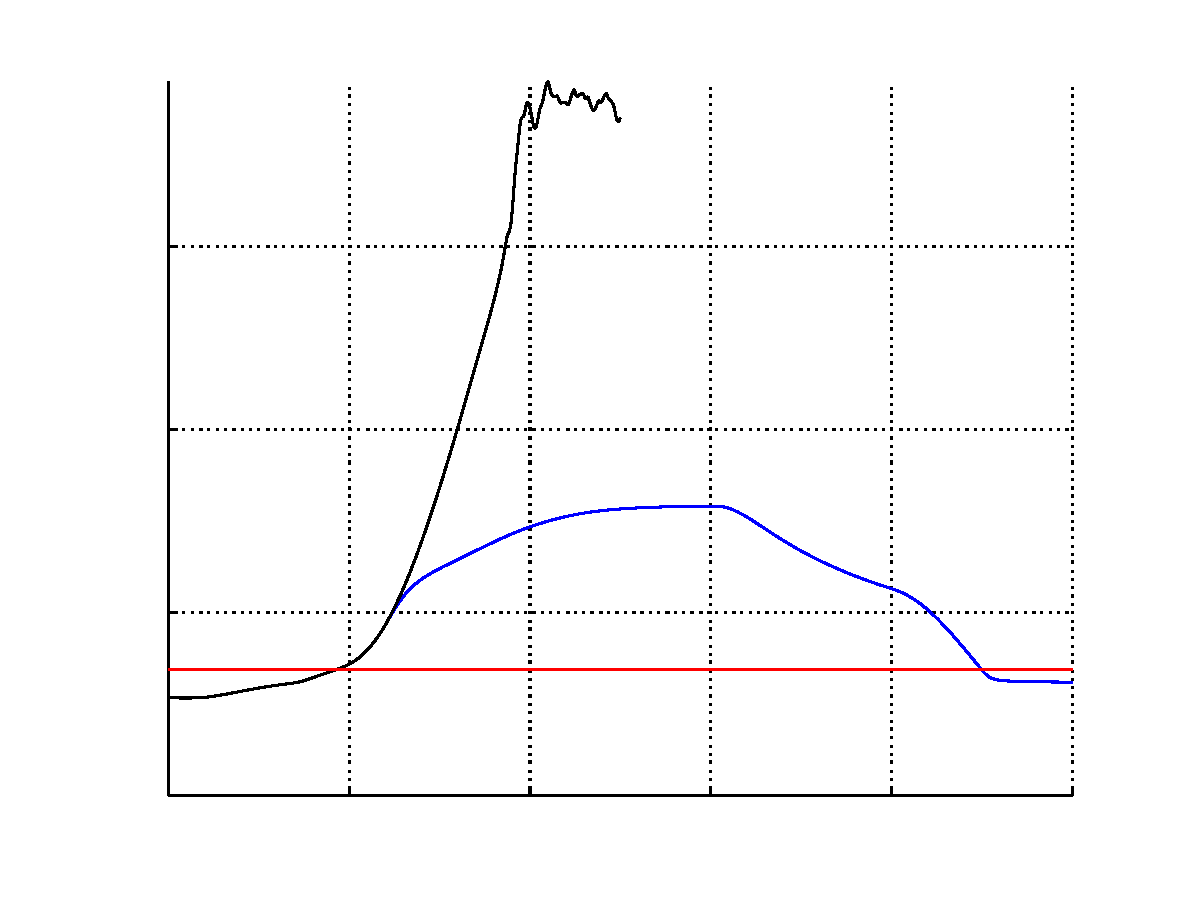
\includegraphics[trim=0  0  0  0,clip,scale=0.6]{test_17_23_com-inc}
\end{picture}%
\begin{picture}(560, 420)(0,0)
\fontsize{11}{0}
\selectfont\put(72.8,41.1956){\makebox(0,0)[t]{\textcolor[rgb]{0,0,0}{{0}}}}
\fontsize{11}{0}
\selectfont\put(159.6,41.1956){\makebox(0,0)[t]{\textcolor[rgb]{0,0,0}{{5}}}}
\fontsize{11}{0}
\selectfont\put(246.4,41.1956){\makebox(0,0)[t]{\textcolor[rgb]{0,0,0}{{10}}}}
\fontsize{11}{0}
\selectfont\put(333.2,41.1956){\makebox(0,0)[t]{\textcolor[rgb]{0,0,0}{{15}}}}
\fontsize{11}{0}
\selectfont\put(420,41.1956){\makebox(0,0)[t]{\textcolor[rgb]{0,0,0}{{20}}}}
\fontsize{11}{0}
\selectfont\put(506.8,41.1956){\makebox(0,0)[t]{\textcolor[rgb]{0,0,0}{{25}}}}
\fontsize{11}{0}
\selectfont\put(67.8,46.2){\makebox(0,0)[r]{\textcolor[rgb]{0,0,0}{{0}}}}
\fontsize{11}{0}
\selectfont\put(67.8,134.023){\makebox(0,0)[r]{\textcolor[rgb]{0,0,0}{{0.1}}}}
\fontsize{11}{0}
\selectfont\put(67.8,221.845){\makebox(0,0)[r]{\textcolor[rgb]{0,0,0}{{0.2}}}}
\fontsize{11}{0}
\selectfont\put(67.8,309.668){\makebox(0,0)[r]{\textcolor[rgb]{0,0,0}{{0.3}}}}
\fontsize{11}{0}
\selectfont\put(289.8,25.1956){\makebox(0,0)[t]{\textcolor[rgb]{0,0,0}{{simulation time $[s]$}}}}
\fontsize{11}{0}
\selectfont\put(43.8,217.35){\rotatebox{90}{\makebox(0,0)[b]{\textcolor[rgb]{0,0,0}{{\ac{CoM} position $[m]$}}}}}
\end{picture}

            \subcaption{
                Position of the \ac{CoM} along the $x$ axis. Position indicated
                with solid blue line corresponds to the controller with the
                capturability constraint. Solid black line indicates position of
                the \ac{CoM} produced by the controller without the
                capturability constraint.
            }
            \label{fig.force_distrib_task_com}
        }
    \end{minipage}
    \caption[Optional contact force: reaching task.]{
        Exploitation of the optional hand contact while performing a right hand
        task.
    }
    \label{fig.force_distrib_task_force_com}
\end{figure}


\begin{figure}[!htbp]
    \begin{minipage}[t]{\textwidth}
        \centering{
            % Title: glps_renderer figure
% Creator: GL2PS 1.3.8, (C) 1999-2012 C. Geuzaine
% For: Octave
% CreationDate: Thu Mar 24 00:51:16 2016
\setlength{\unitlength}{0.6pt}
\begin{picture}(0,0)
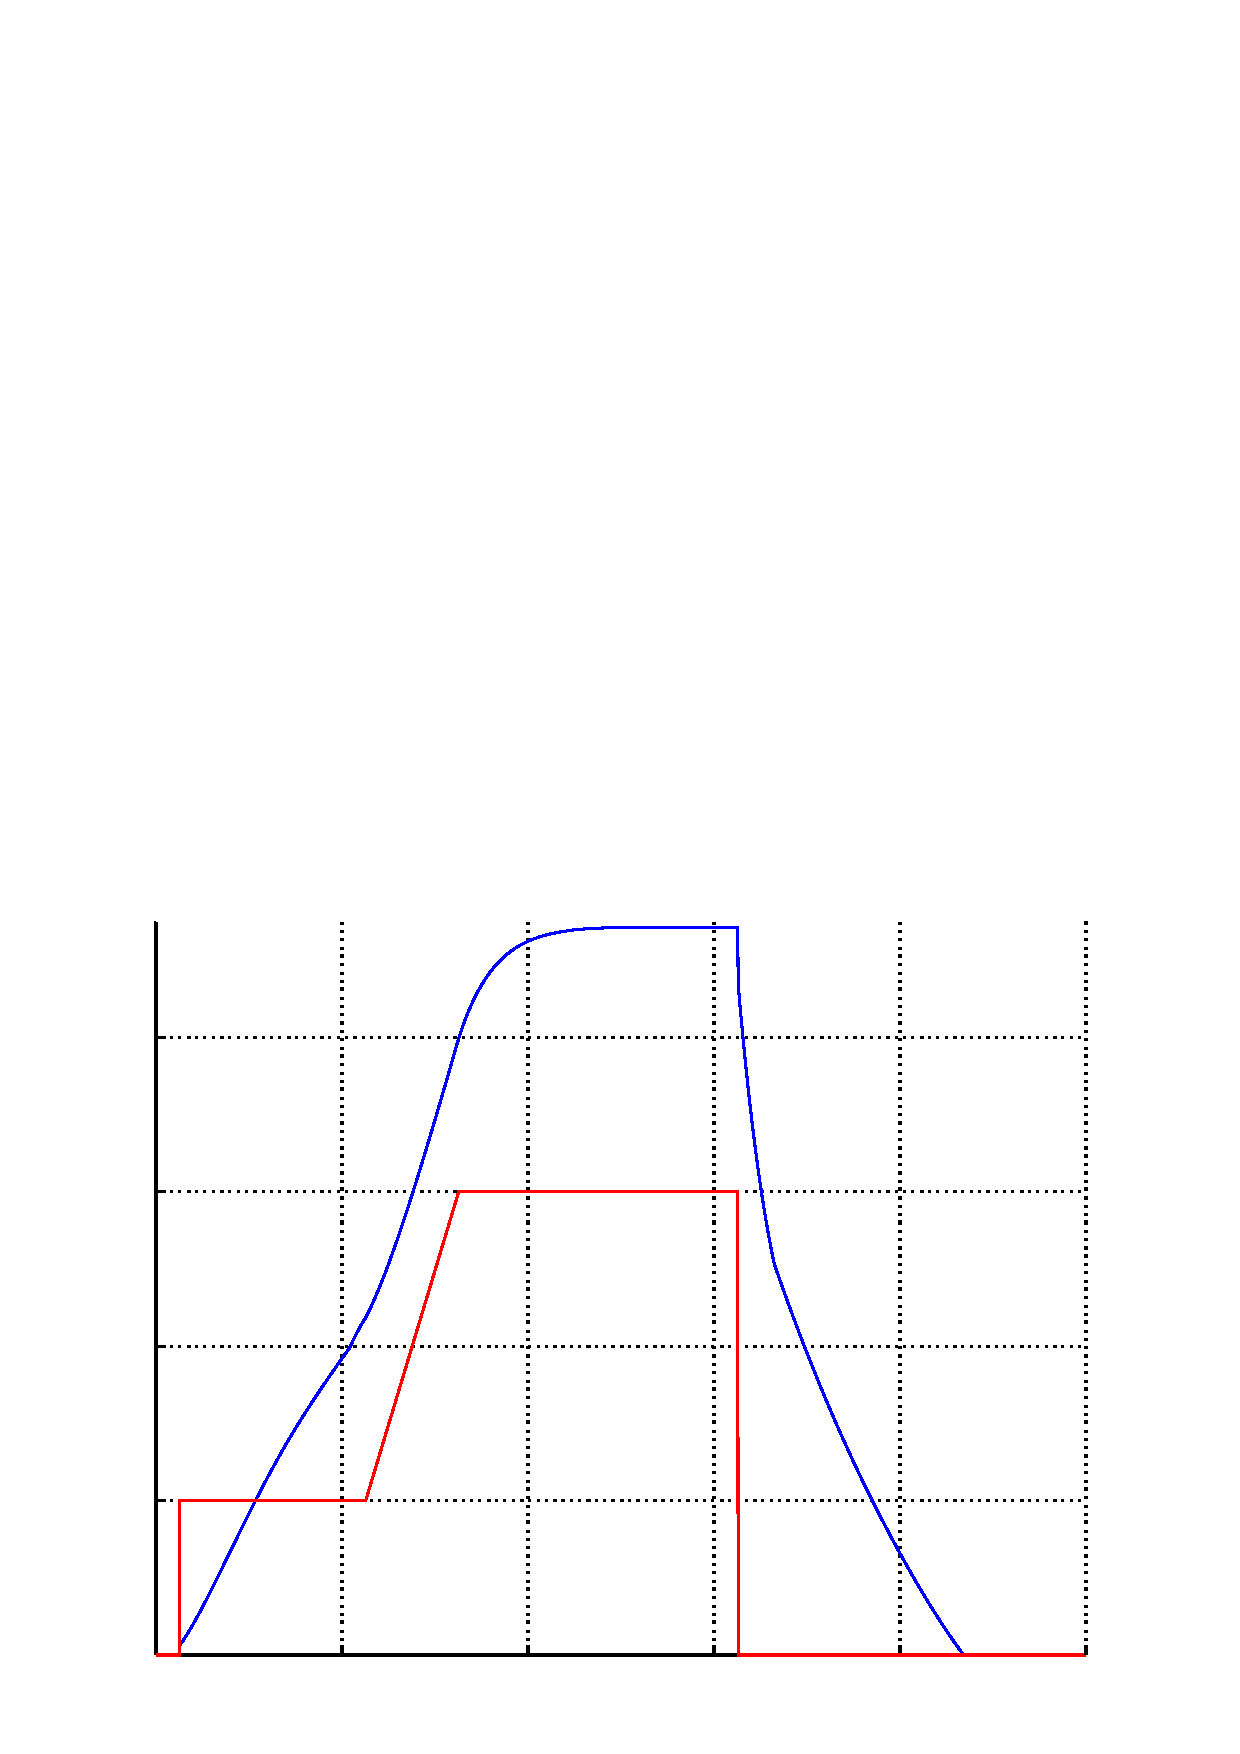
\includegraphics[trim=0  0  0  0,clip,scale=0.6]{test_17_24_force-inc}
\end{picture}%
\begin{picture}(576, 432)(0,0)
\fontsize{11}{0}
\selectfont\put(74.88,42.5189){\makebox(0,0)[t]{\textcolor[rgb]{0,0,0}{{0}}}}
\fontsize{11}{0}
\selectfont\put(164.16,42.5189){\makebox(0,0)[t]{\textcolor[rgb]{0,0,0}{{2}}}}
\fontsize{11}{0}
\selectfont\put(253.44,42.5189){\makebox(0,0)[t]{\textcolor[rgb]{0,0,0}{{4}}}}
\fontsize{11}{0}
\selectfont\put(342.72,42.5189){\makebox(0,0)[t]{\textcolor[rgb]{0,0,0}{{6}}}}
\fontsize{11}{0}
\selectfont\put(432,42.5189){\makebox(0,0)[t]{\textcolor[rgb]{0,0,0}{{8}}}}
\fontsize{11}{0}
\selectfont\put(521.28,42.5189){\makebox(0,0)[t]{\textcolor[rgb]{0,0,0}{{10}}}}
\fontsize{11}{0}
\selectfont\put(69.8755,47.52){\makebox(0,0)[r]{\textcolor[rgb]{0,0,0}{{0}}}}
\fontsize{11}{0}
\selectfont\put(69.8755,121.642){\makebox(0,0)[r]{\textcolor[rgb]{0,0,0}{{20}}}}
\fontsize{11}{0}
\selectfont\put(69.8755,195.764){\makebox(0,0)[r]{\textcolor[rgb]{0,0,0}{{40}}}}
\fontsize{11}{0}
\selectfont\put(69.8755,269.886){\makebox(0,0)[r]{\textcolor[rgb]{0,0,0}{{60}}}}
\fontsize{11}{0}
\selectfont\put(69.8755,344.008){\makebox(0,0)[r]{\textcolor[rgb]{0,0,0}{{80}}}}
\fontsize{11}{0}
\selectfont\put(298.08,26.5189){\makebox(0,0)[t]{\textcolor[rgb]{0,0,0}{{simulation time $[s]$}}}}
\fontsize{11}{0}
\selectfont\put(49.8755,223.56){\rotatebox{90}{\makebox(0,0)[b]{\textcolor[rgb]{0,0,0}{{forces $[N]$}}}}}
\end{picture}

            \subcaption{
                Norms of the optional left hand contact force
                $\V{f}_{0,\MT{lh}}$ (solid blue) and the disturbing external
                force $\V{f}_{\MT{rh}}$ (solid red).
            }
            \label{fig.force_distrib_weight_force}
        }
    \end{minipage}
    \begin{minipage}[t]{\textwidth}
        \centering{
            % Title: glps_renderer figure
% Creator: GL2PS 1.3.8, (C) 1999-2012 C. Geuzaine
% For: Octave
% CreationDate: Thu Mar 24 00:51:17 2016
\setlength{\unitlength}{0.6pt}
\begin{picture}(0,0)
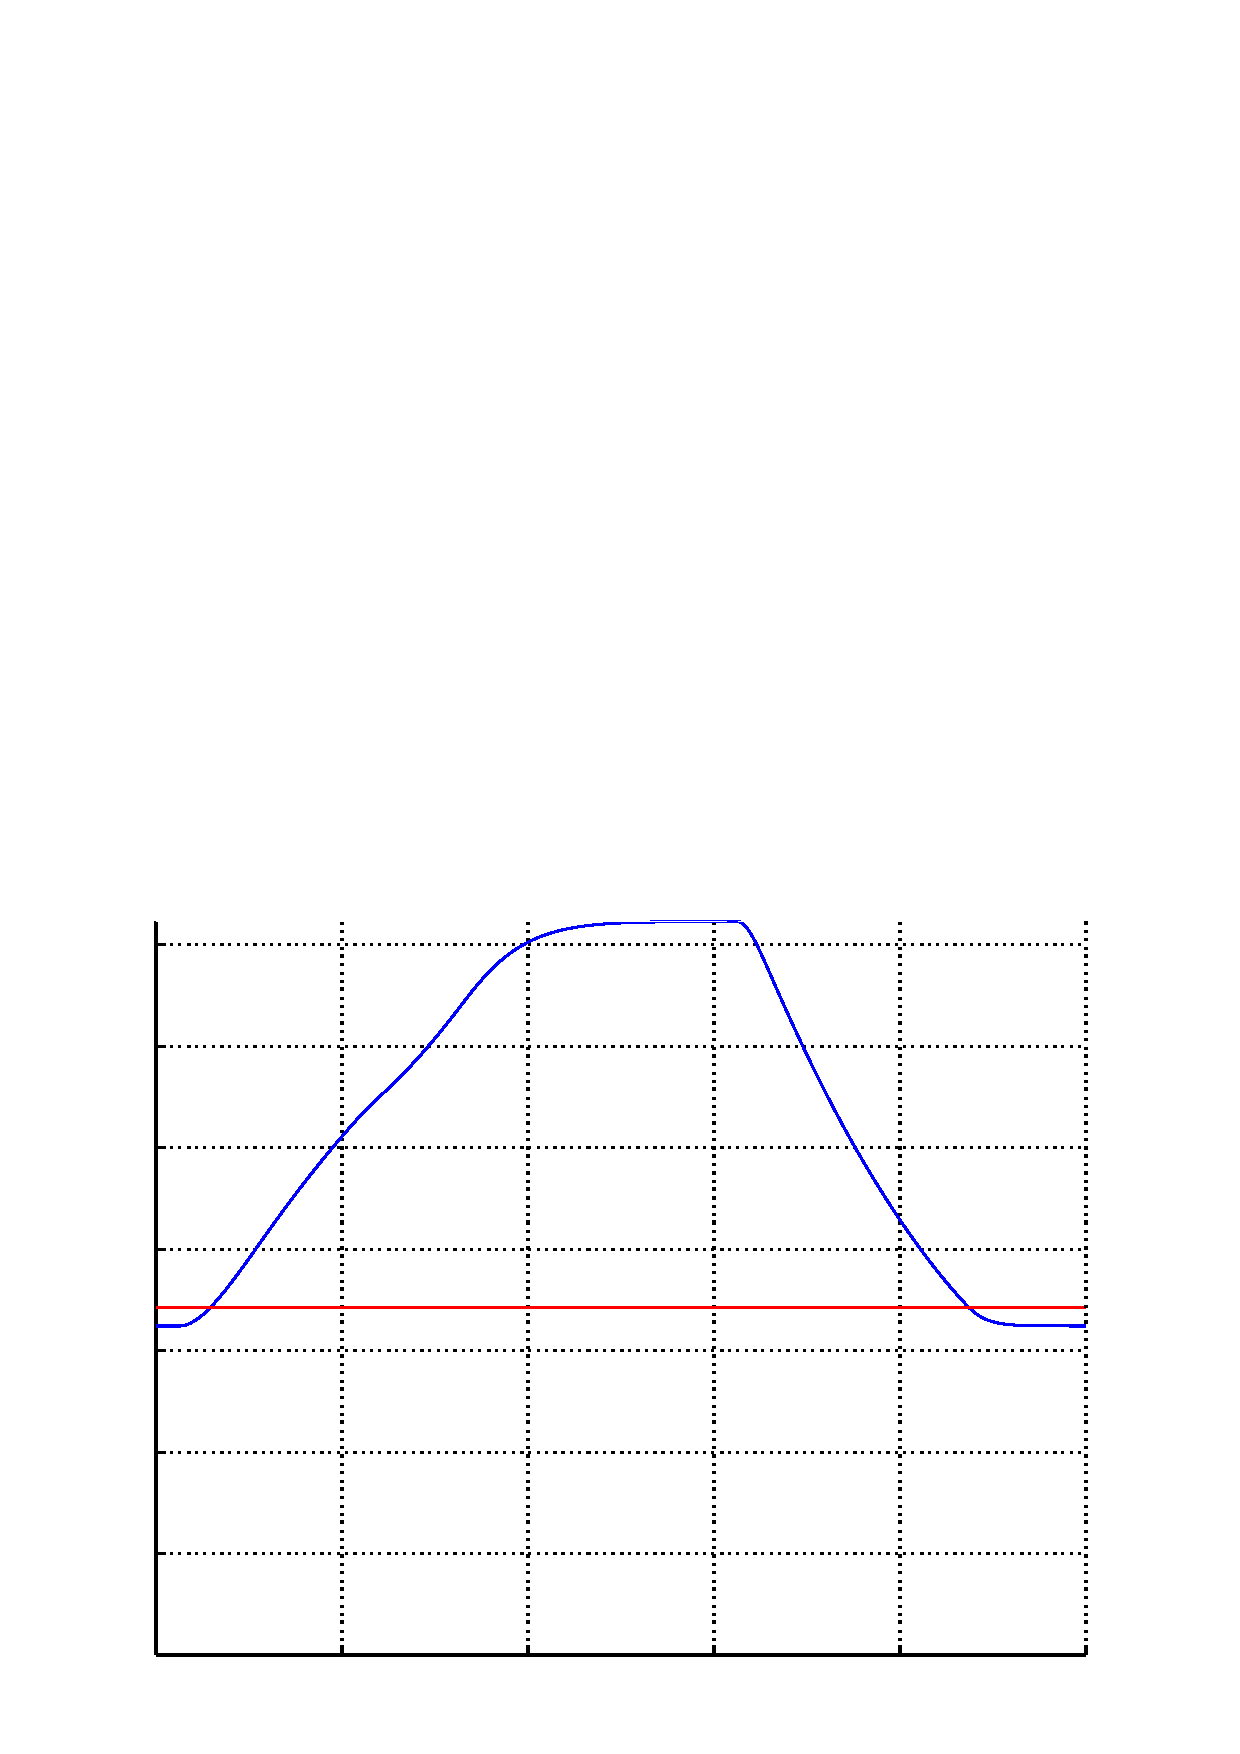
\includegraphics[trim=0  0  0  0,clip,scale=0.6]{test_17_24_com-inc}
\end{picture}%
\begin{picture}(576, 432)(0,0)
\fontsize{11}{0}
\selectfont\put(74.88,42.5189){\makebox(0,0)[t]{\textcolor[rgb]{0,0,0}{{0}}}}
\fontsize{11}{0}
\selectfont\put(164.16,42.5189){\makebox(0,0)[t]{\textcolor[rgb]{0,0,0}{{2}}}}
\fontsize{11}{0}
\selectfont\put(253.44,42.5189){\makebox(0,0)[t]{\textcolor[rgb]{0,0,0}{{4}}}}
\fontsize{11}{0}
\selectfont\put(342.72,42.5189){\makebox(0,0)[t]{\textcolor[rgb]{0,0,0}{{6}}}}
\fontsize{11}{0}
\selectfont\put(432,42.5189){\makebox(0,0)[t]{\textcolor[rgb]{0,0,0}{{8}}}}
\fontsize{11}{0}
\selectfont\put(521.28,42.5189){\makebox(0,0)[t]{\textcolor[rgb]{0,0,0}{{10}}}}
\fontsize{11}{0}
\selectfont\put(69.8755,47.52){\makebox(0,0)[r]{\textcolor[rgb]{0,0,0}{{0}}}}
\fontsize{11}{0}
\selectfont\put(69.8755,96.2139){\makebox(0,0)[r]{\textcolor[rgb]{0,0,0}{{0.02}}}}
\fontsize{11}{0}
\selectfont\put(69.8755,144.908){\makebox(0,0)[r]{\textcolor[rgb]{0,0,0}{{0.04}}}}
\fontsize{11}{0}
\selectfont\put(69.8755,193.602){\makebox(0,0)[r]{\textcolor[rgb]{0,0,0}{{0.06}}}}
\fontsize{11}{0}
\selectfont\put(69.8755,242.295){\makebox(0,0)[r]{\textcolor[rgb]{0,0,0}{{0.08}}}}
\fontsize{11}{0}
\selectfont\put(69.8755,290.989){\makebox(0,0)[r]{\textcolor[rgb]{0,0,0}{{0.1}}}}
\fontsize{11}{0}
\selectfont\put(69.8755,339.683){\makebox(0,0)[r]{\textcolor[rgb]{0,0,0}{{0.12}}}}
\fontsize{11}{0}
\selectfont\put(69.8755,388.377){\makebox(0,0)[r]{\textcolor[rgb]{0,0,0}{{0.14}}}}
\fontsize{11}{0}
\selectfont\put(298.08,26.5189){\makebox(0,0)[t]{\textcolor[rgb]{0,0,0}{{simulation time $[s]$}}}}
\fontsize{11}{0}
\selectfont\put(37.8755,223.56){\rotatebox{90}{\makebox(0,0)[b]{\textcolor[rgb]{0,0,0}{{\ac{CoM} position $[m]$}}}}}
\end{picture}

            \subcaption{
                Position of the \ac{CoM} along the $x$ axis (solid blue) and
                the bound of the foot support area (solid red).
            }
            \label{fig.force_distrib_weight_com}
        }
    \end{minipage}
    \caption[Optional contact force: disturbing force.]{
        Exploitation of the optional hand contact in presence of external
        disturbing force.
    }
    \label{fig.force_distrib_weight_force_com}
\end{figure}



\begin{figure}[!htbp]
    \centering{
        \input{test_17_23_joints.tex}
        \caption[Chattering of the joint accelerations.]{
            Accelerations of the right arm joints without regularization (top)
            and with it (bottom).
        }
        \label{fig.chattering}
    }
\end{figure}



\begin{figure}[!htbp]
    \centering{
        % Title: glps_renderer figure
% Creator: GL2PS 1.3.8, (C) 1999-2012 C. Geuzaine
% For: Octave
% CreationDate: Mon May  9 19:44:34 2016
\setlength{\unitlength}{0.7pt}
\begin{picture}(0,0)
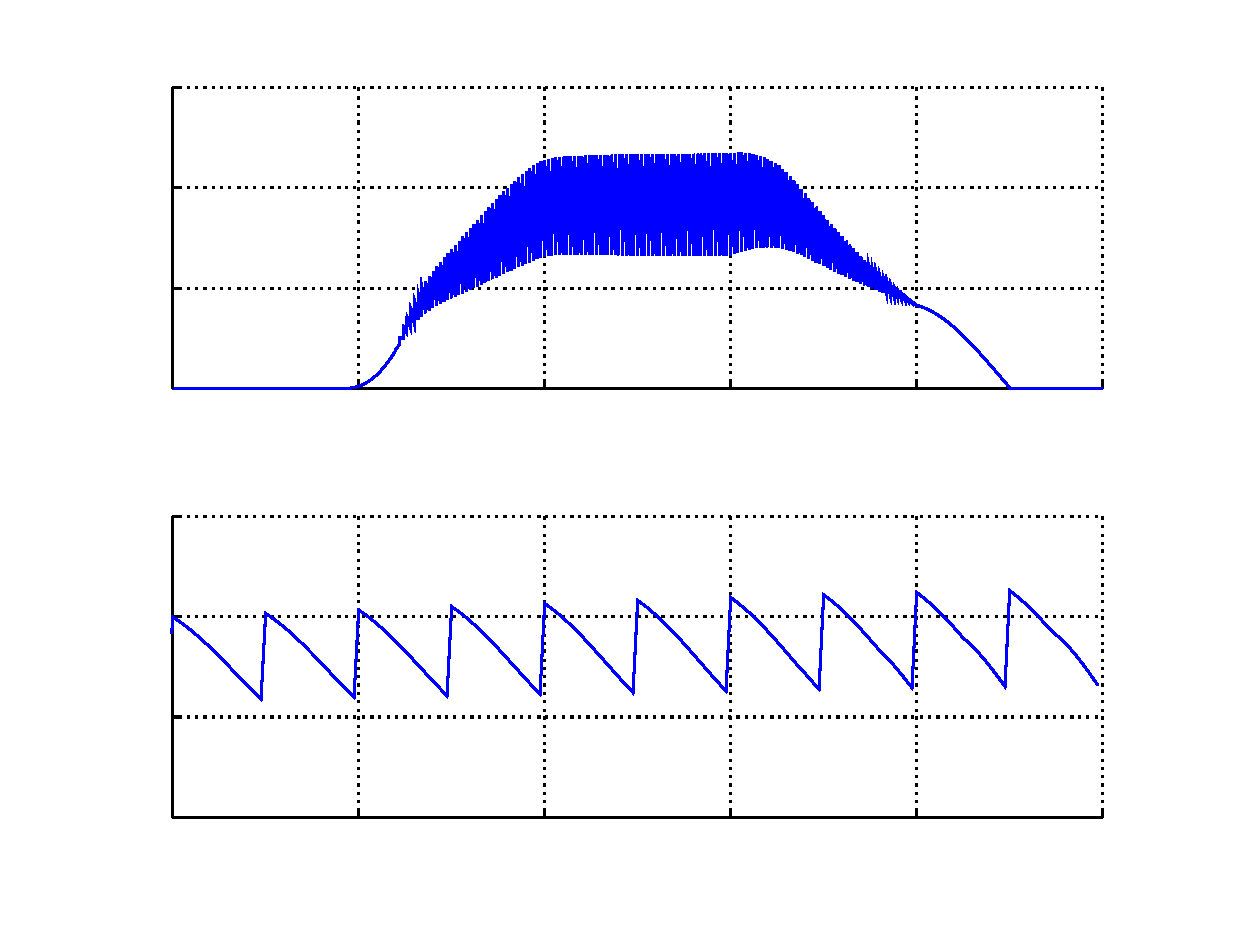
\includegraphics[trim=0  0  0  0,clip,scale=0.7]{test_17_23_badmpc_force-inc}
\end{picture}%
\begin{picture}(576, 432)(0,0)
\fontsize{11}{0}
\selectfont\put(74.88,248.382){\makebox(0,0)[t]{\textcolor[rgb]{0,0,0}{{0}}}}
\fontsize{11}{0}
\selectfont\put(164.16,248.382){\makebox(0,0)[t]{\textcolor[rgb]{0,0,0}{{5}}}}
\fontsize{11}{0}
\selectfont\put(253.44,248.382){\makebox(0,0)[t]{\textcolor[rgb]{0,0,0}{{10}}}}
\fontsize{11}{0}
\selectfont\put(342.72,248.382){\makebox(0,0)[t]{\textcolor[rgb]{0,0,0}{{15}}}}
\fontsize{11}{0}
\selectfont\put(432,248.382){\makebox(0,0)[t]{\textcolor[rgb]{0,0,0}{{20}}}}
\fontsize{11}{0}
\selectfont\put(521.28,248.382){\makebox(0,0)[t]{\textcolor[rgb]{0,0,0}{{25}}}}
\fontsize{11}{0}
\selectfont\put(69.8755,253.397){\makebox(0,0)[r]{\textcolor[rgb]{0,0,0}{{0}}}}
\fontsize{11}{0}
\selectfont\put(69.8755,301.544){\makebox(0,0)[r]{\textcolor[rgb]{0,0,0}{{40}}}}
\fontsize{11}{0}
\selectfont\put(69.8755,349.691){\makebox(0,0)[r]{\textcolor[rgb]{0,0,0}{{80}}}}
\fontsize{11}{0}
\selectfont\put(69.8755,397.837){\makebox(0,0)[r]{\textcolor[rgb]{0,0,0}{{120}}}}
\fontsize{11}{0}
\selectfont\put(41.8755,325.617){\rotatebox{90}{\makebox(0,0)[b]{\textcolor[rgb]{0,0,0}{{$\force_{0,\MT{lh}}$ $[N]$}}}}}
\fontsize{11}{0}
\selectfont\put(74.88,42.5047){\makebox(0,0)[t]{\textcolor[rgb]{0,0,0}{{9}}}}
\fontsize{11}{0}
\selectfont\put(164.16,42.5047){\makebox(0,0)[t]{\textcolor[rgb]{0,0,0}{{9.2}}}}
\fontsize{11}{0}
\selectfont\put(253.44,42.5047){\makebox(0,0)[t]{\textcolor[rgb]{0,0,0}{{9.4}}}}
\fontsize{11}{0}
\selectfont\put(342.72,42.5047){\makebox(0,0)[t]{\textcolor[rgb]{0,0,0}{{9.6}}}}
\fontsize{11}{0}
\selectfont\put(432,42.5047){\makebox(0,0)[t]{\textcolor[rgb]{0,0,0}{{9.8}}}}
\fontsize{11}{0}
\selectfont\put(521.28,42.5047){\makebox(0,0)[t]{\textcolor[rgb]{0,0,0}{{10}}}}
\fontsize{11}{0}
\selectfont\put(69.8757,47.52){\makebox(0,0)[r]{\textcolor[rgb]{0,0,0}{{0}}}}
\fontsize{11}{0}
\selectfont\put(69.8757,95.6667){\makebox(0,0)[r]{\textcolor[rgb]{0,0,0}{{40}}}}
\fontsize{11}{0}
\selectfont\put(69.8757,143.813){\makebox(0,0)[r]{\textcolor[rgb]{0,0,0}{{80}}}}
\fontsize{11}{0}
\selectfont\put(69.8757,191.96){\makebox(0,0)[r]{\textcolor[rgb]{0,0,0}{{120}}}}
\fontsize{11}{0}
\selectfont\put(298.08,26.5047){\makebox(0,0)[t]{\textcolor[rgb]{0,0,0}{{simulation time $[s]$}}}}
\fontsize{11}{0}
\selectfont\put(41.8756,119.74){\rotatebox{90}{\makebox(0,0)[b]{\textcolor[rgb]{0,0,0}{{$\force_{0,\MT{lh}}$ $[N]$}}}}}
\end{picture}

        \caption[Periodic variations in the norm of the optional contact force.]{
            Norm of the optional left hand contact force when the first
            sampling interval is reduced at each control iteration.
        }
        \label{fig.subsampling}
    }
\end{figure}




%%%%%%%%%%%%%%%%%%%%%%%%%%%%%%%%%%%%%%%%%%%%%%%%%%%%%%%%%%%%%%%%%%%%%%%%%%%%%%%%
\subsection{Conclusion}\label{sec.force_conclusion}

An interesting property of the constructed controller is that the decision to
apply the optional contact force is taken automatically based on the current
state and tasks. Hence, there is no need for planning and tuning of contact
timings, which are recognized as a significant drawback of approximate linear
models \cite{Audren2014iros}. On the other hand, the considered setting is very
limited: the contact positions are known and fixed in advance. Extensibility of
the approach to more general situations is to be investigated.


One potential application of the controller could be evaluation of necessity of
an optional contact for balance preservation in the future. For example, when
the robot is pushed, the controller may decide if using an additional hand
contact with a wall at some time $t$ in the future would be necessary to avoid
a fall. If so, an appropriate task can be triggered to move the hand towards
the wall.


We believe that the current primary obstacle for adoption of the proposed
approach is the lack of numerical tools, which can solve hierarchies both
efficiently and accurately. The size of \cref{hr.mmpc_force} makes its solution
with a sequence of \acs{QP}s impractical. At the same time, the existing
specialized solvers for hierarchies, \sn{LexLS} \cite{Dimitrov2015preprint} and
\sn{SOTH} \cite{Escande2014ijrr, SOTHsite}, provide very limited mechanisms for
coping with the numerical problems near singularities discussed in
\cref{sec.force_results}. Since singularities commonly arise due to conflicts
in hierarchies, it is necessary to develop and extend these mechanisms in order
to maximally benefit from prioritization. For example, it is desirable to have
regularization with general equality objective with automatic selection of the
regularization factor (see \cref{sec.regularization}).



%%%%%%%%%%%%%%%%%%%%%%%%%%%%%%%%%%%%%%%%%%%%%%%%%%%%%%%%%%%%%%%%%%%%%%%%%%%%%%%%
%%%%%%%%%%%%%%%%%%%%%%%%%%%%%%%%%%%%%%%%%%%%%%%%%%%%%%%%%%%%%%%%%%%%%%%%%%%%%%%%
%%%%%%%%%%%%%%%%%%%%%%%%%%%%%%%%%%%%%%%%%%%%%%%%%%%%%%%%%%%%%%%%%%%%%%%%%%%%%%%%
\section{Collaborations}\label{sec.collaboration_results}

A substantial part of the work covered by the present thesis was performed in
collaboration with other doctoral and master students from different research
institutes. The author's contribution to the collaborative works is briefly
outlined in the following subsections.


%%%%%%%%%%%%%%%%%%%%%%%%%%%%%%%%%%%%%%%%%%%%%%%%%%%%%%%%%%%%%%%%%%%%%%%%%%%%%%%%
\subsection{Walking with nonplanar CoM motion}\label{sec.3d_walk}

One of the recurring assumptions made in the construction of linear approximate
models of humanoid robots is that the \ac{CoM} motion is constrained to a plane
(see \cref{ass.fixed_z_coordinate} in \cref{sec.linear_approx_models}). This
limitation is particularly inconvenient when the robot has to walk on uneven
terrain, \IE, when walking up and down stairs. Moreover, even walking on a flat
ground with planar \ac{CoM} motion is unnatural and energy inefficient in
comparison with humans. This issue was addressed in the Master's thesis of
Camille Brasseur, who was, to some extend, co-advised by the author.


Camille's work resulted in the development of an approximate model
\cite{Brasseur2015thesis}, which enables nonplanar motion of the \ac{CoM} at
the price of a larger number of constraints, as indicated in
\cref{sec.point_mass_nonplanar} of this thesis. The obtained model was employed
by Camille in the implementation of an \ac{MPC} scheme for the generation of
walking motions on flat and uneven ground. Since this \ac{MPC} scheme was not
integrated in an \ac{MMPC} controller, the author developed a simple whole body
inverse dynamics controller based on \cref{hr.wbc_controller} for tracking the
generated \ac{CoM} and foot trajectories. The whole body controller was used to
demonstrate the validity of the approach using a simulated \sn{HRP-2} robot.
Snapshots of a simulated walk on stairs are given in \cref{fig.stairs_walk}.
This joint work led to a publication in a conference proceedings
\cite{Brasseur2015humanoids}. Also, the results with detailed derivations were
reported in the corresponding Master's thesis \cite{Brasseur2015thesis}.


%
\begin{figure}[!htb]
    \centering{
        % Title: glps_renderer figure
% Creator: GL2PS 1.3.8, (C) 1999-2012 C. Geuzaine
% For: Octave
% CreationDate: Wed Jun  8 12:43:33 2016
\setlength{\unitlength}{0.9pt}
\begin{picture}(0,0)
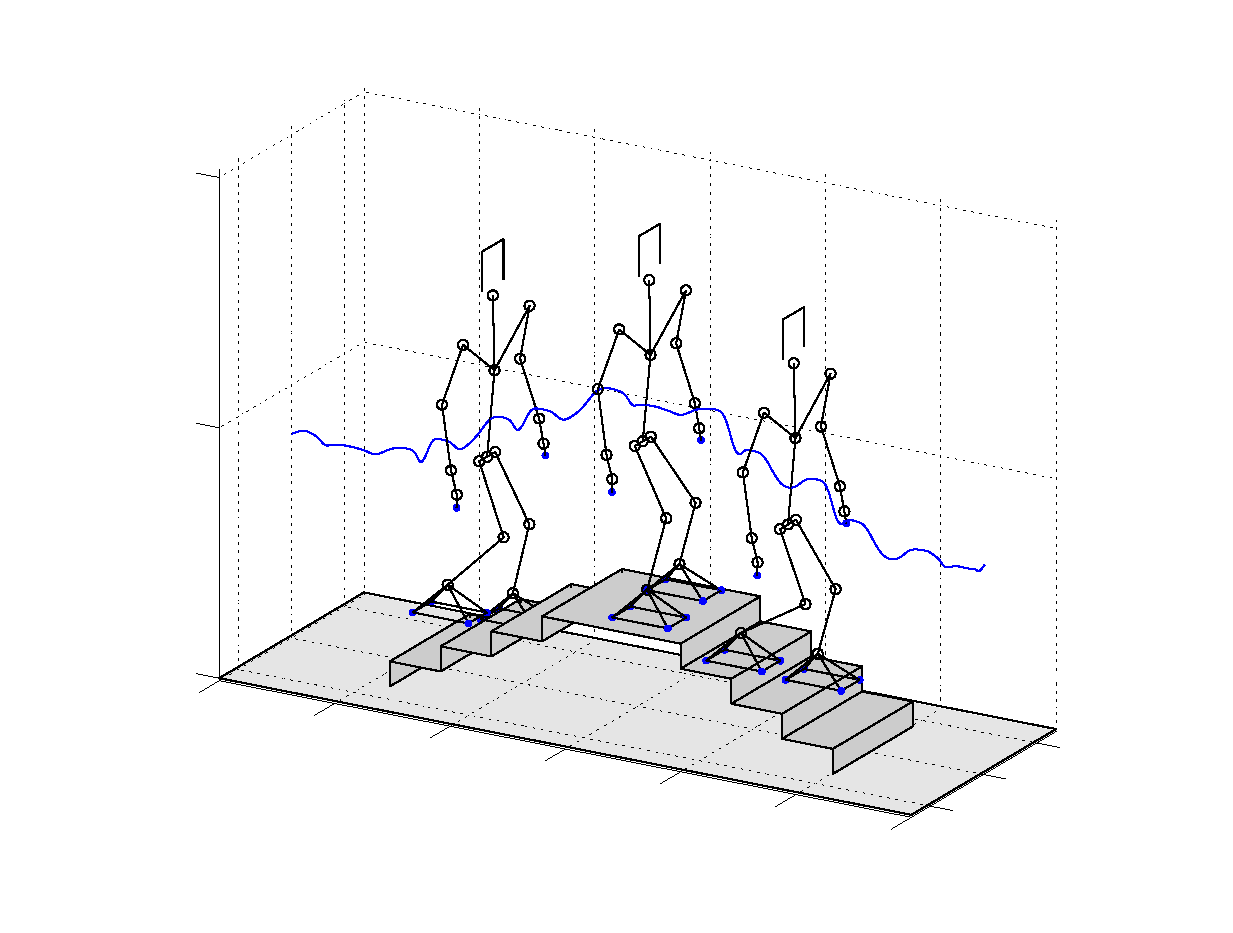
\includegraphics[trim=60  30  50   5,clip,scale=0.9]{test_16_16_robot_on_stairs-inc}
\end{picture}%
\begin{picture}(466, 397)(60,30)
\fontsize{10}{0}
\selectfont\put(81.3775,117.452){\makebox(0,0)[br]{\textcolor[rgb]{0,0,0}{{0}}}}
\fontsize{10}{0}
\selectfont\put(81.3775,237.605){\makebox(0,0)[br]{\textcolor[rgb]{0,0,0}{{1}}}}
\fontsize{10}{0}
\selectfont\put(81.3775,357.759){\makebox(0,0)[br]{\textcolor[rgb]{0,0,0}{{2}}}}
\fontsize{10}{0}
\selectfont\put(83.2472,104.831){\makebox(0,0)[tr]{\textcolor[rgb]{0,0,0}{{0}}}}
\fontsize{10}{0}
\selectfont\put(138.614,93.8979){\makebox(0,0)[tr]{\textcolor[rgb]{0,0,0}{{0.5}}}}
\fontsize{10}{0}
\selectfont\put(209.382,299.759){\makebox(0,0)[l]{\textcolor[rgb]{0,0,0}{{(1)}}}}
\fontsize{10}{0}
\selectfont\put(193.981,82.9648){\makebox(0,0)[tr]{\textcolor[rgb]{0,0,0}{{1}}}}
\fontsize{10}{0}
\selectfont\put(249.348,72.0317){\makebox(0,0)[tr]{\textcolor[rgb]{0,0,0}{{1.5}}}}
\fontsize{10}{0}
\selectfont\put(281.359,309.577){\makebox(0,0)[l]{\textcolor[rgb]{0,0,0}{{(2)}}}}
\fontsize{10}{0}
\selectfont\put(304.716,61.0986){\makebox(0,0)[tr]{\textcolor[rgb]{0,0,0}{{2}}}}
\fontsize{10}{0}
\selectfont\put(360.083,50.1655){\makebox(0,0)[tr]{\textcolor[rgb]{0,0,0}{{2.5}}}}
\fontsize{10}{0}
\selectfont\put(415.45,39.2325){\makebox(0,0)[tr]{\textcolor[rgb]{0,0,0}{{3}}}}
\fontsize{10}{0}
\selectfont\put(454.357,49.7542){\makebox(0,0)[tl]{\textcolor[rgb]{0,0,0}{{-0.4}}}}
\fontsize{10}{0}
\selectfont\put(479.93,64.9035){\makebox(0,0)[tl]{\textcolor[rgb]{0,0,0}{{0}}}}
\fontsize{10}{0}
\selectfont\put(505.503,80.0528){\makebox(0,0)[tl]{\textcolor[rgb]{0,0,0}{{0.4}}}}
\fontsize{10}{0}
\selectfont\put(353.336,271.333){\makebox(0,0)[l]{\textcolor[rgb]{0,0,0}{{(3)}}}}
\end{picture}

        \caption[Robot walking up and down stairs.]{
            Robot walking up and down stairs. Sequence of the snapshots is
            indicated by the numbers. Blue curve indicates nonplanar trajectory
            of the \ac{CoM}.
        }
        \label{fig.stairs_walk}
    }
\end{figure}
%


%%%%%%%%%%%%%%%%%%%%%%%%%%%%%%%%%%%%%%%%%%%%%%%%%%%%%%%%%%%%%%%%%%%%%%%%%%%%%%%%
\subsection{Time-optimal control of industrial manipulators}\label{sec.time_opt}

The idea of time-optimal control using the temporal task prioritization in an
\acs{MPC} problem, as described in \cref{sec.time_optimal_mpc}, was proposed by
the author to another doctoral student, Saed Al Homsi, who performed research
in time-optimal control of industrial manipulators. One of the goals of Saed's
work was to reduce involvement of humans in deployment of industrial robots
operating in a shared environment. One of the problems, which must be faced in
such setups, is collision avoidance between the robots (see \cref{fig.cobra}).
This can be achieved by designing an \ac{MPC} scheme with appropriate
constraints on positions of the links of the manipulator. At the same time,
addition of task prioritization in this \ac{MPC} problem allows for
time-optimal behavior, which is valuable in industrial applications. The
obtained \ac{PLLS} optimization problem can be solved using \sn{LexLS} or
another specialized solver.

Based on the proposed approach to time-optimal control, Saed developed a
real-time controller for Adept Cobra \acs{SCARA} manipulators \cite{ADEPTsite}
and validated it on real robots in the experimental setup visualized in
\cref{fig.cobra}. Results of the experiments with additional simulations and
overview of the concept were published in \cite{alHomsi2016icra}, an interested
reader can find further details in Saed's dissertation
\cite{alHomsi2016thesis}.


%
\begin{figure}[!htb]
    \begin{minipage}[t]{0.49\textwidth}
        \centering{
            \includegraphics[scale=0.25]{cobra_1.eps}\\
            (1)
            \vspace{0.2cm}
        }
    \end{minipage}
    \hfill
    \begin{minipage}[t]{0.49\textwidth}
        \centering{
            \includegraphics[scale=0.25]{cobra_2.eps}\\
            (2)
            \vspace{0.2cm}
        }
    \end{minipage}
    \begin{minipage}[t]{0.49\textwidth}
        \centering{
            \includegraphics[scale=0.25]{cobra_3.eps}\\
            (3)
        }
    \end{minipage}
    \hfill
    \begin{minipage}[t]{0.49\textwidth}
        \centering{
            \includegraphics[scale=0.25]{cobra_4.eps}\\
            (4)
        }
    \end{minipage}
    \caption[Industrial manipulators in a shared environment.]{
        Two Adept Cobra \acs{SCARA} robots \cite{ADEPTsite} operating in a
        shared environment. The robots have to reach targets, indicated by
        colored cylinders, on two conveyors. A target for a particular robot
        may appear on either of the conveyors. In order to realize the tasks,
        the robots have to avoid collisions with each other.
    }
    \label{fig.cobra}
\end{figure}
%



%%%%%%%%%%%%%%%%%%%%%%%%%%%%%%%%%%%%%%%%%%%%%%%%%%%%%%%%%%%%%%%%%%%%%%%%%%%%%%%%
\subsection{Physical human-robot collaboration for carrying}\label{sec.robot_collaboration}

The execution of certain tasks may require physical collaboration of robots
with each other or with humans \cite{Caccavale2008handbook,
Bicchi2008handbook}. Humanoid robots are not an exception
\cite{Agravante2016preprint}. For example, they can assist humans in carrying
heavy or bulky objects, as shown in
\cref{fig.collaboration_box,fig.collaboration_stretcher}. The realization of
such collaboration was the goal of Joven Agravante during his Doctoral research
at LIRMM in Montpellier.


The transportation of an object requires walking and, hence, motion
anticipation, which must take into account two important aspects of physical
collaboration between the human and the robot:
%
\begin{itemize}
    \item it is necessary to account for the interaction forces exerted on the
        robot in order to maintain balance;

    \item it is necessary to react to human intentions conveyed through the
        interaction forces by adjusting motions of the robot appropriately, in
        particular, by adjusting its waking speed.
\end{itemize}
%
Joven addressed both of these aspects by developing the approximate
\nameref{model.CPPMJ} model, which incorporates the external wrench
$(\forceext, \momentext)$ acting on the \ac{CoM} of the robot. Thus, the
estimated interaction force applied to the \ac{CoM} is taken into account in
the balance preservation constraints and can influence the motion of the
\ac{CoM} through an impedance task of the following form
%
\begin{equation}
    \forceext^{xy}
    =
    \M{\Gamma}_{\V{x}}
    \V{x},
\end{equation}
%
where $\M{\Gamma}_{\V{x}}$ is an appropriately chosen matrix and the state of
the model is $\V{x} = (\C{c}^x, \dotC{c}^x, \ddotC{c}^x, \C{c}^y, \dotC{c}^y,
\ddotC{c}^y)$. The obtained model was employed in an \ac{MPC} scheme for
the generation of walking motions of an \sn{HRP-4} robot \cite{Kaneko2011iros}, as
illustrated in \cref{fig.collaboration_box,fig.collaboration_stretcher}. In
order to attain real-time performance of this scheme it was implemented by
Joven in \sn{C++} using the software framework \sn{HuMoTo}, which was designed and
partially implemented by the author. Experimental and theoretical results of
this work were reported in \cite{Agravante2016preprint, Agravante2016icra} and
Joven's thesis \cite{Agravante2015thesis}.


\begin{figure}[!htb]
    \begin{minipage}[t]{0.49\textwidth}
        \centering{
            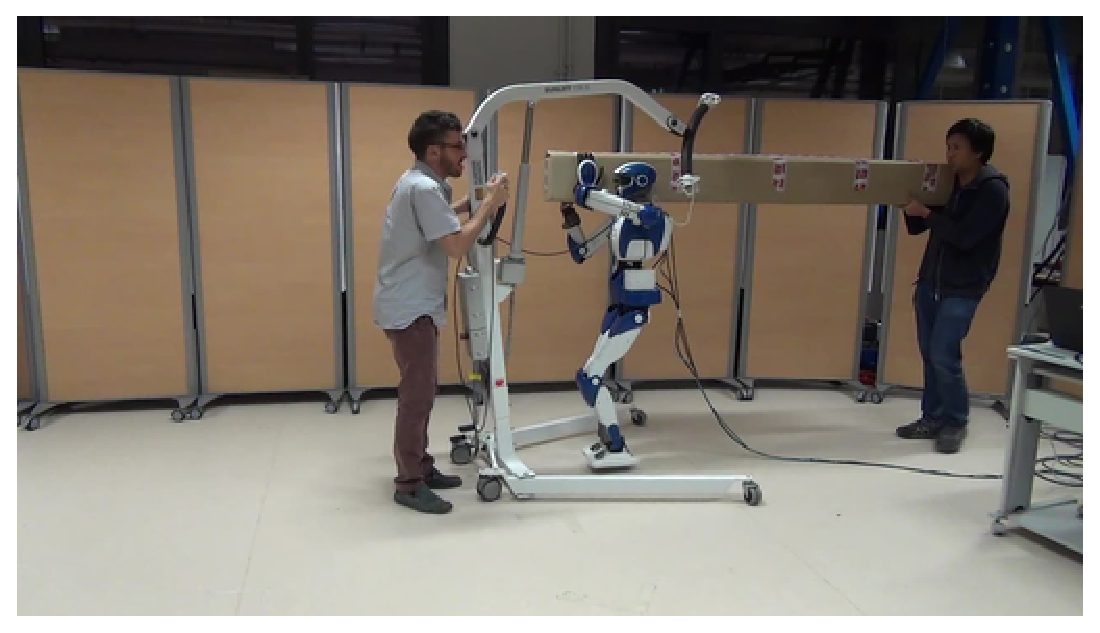
\includegraphics[scale=0.4]{collaboration_box2.eps}\\
            (1)
            \vspace{0.2cm}
        }
    \end{minipage}
    \hfill
    \begin{minipage}[t]{0.49\textwidth}
        \centering{
            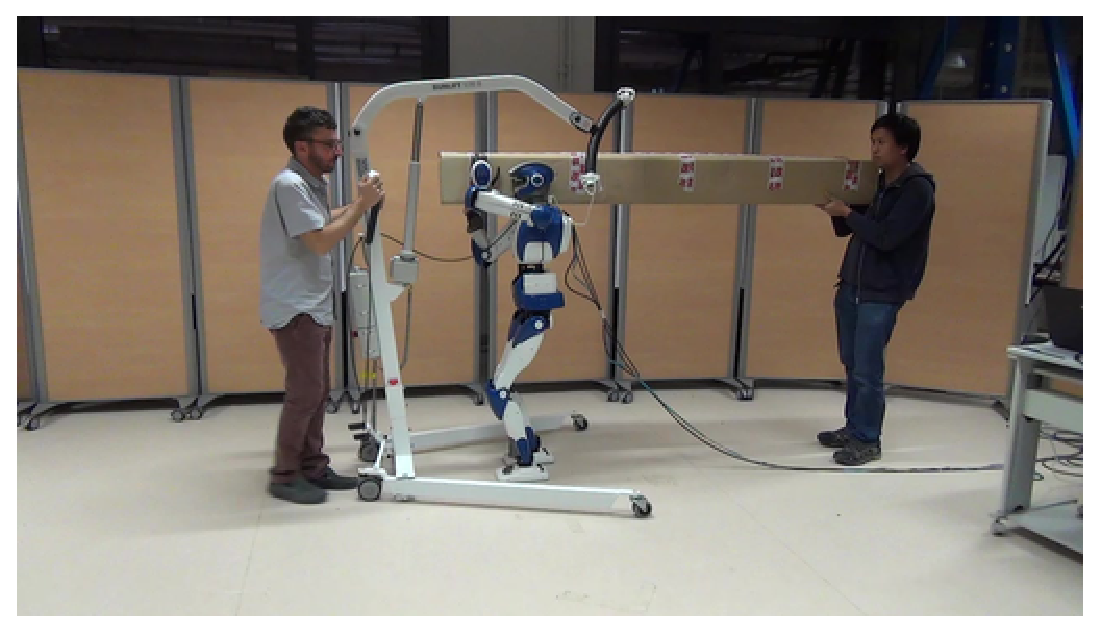
\includegraphics[scale=0.4]{collaboration_box3.eps}\\
            (2)
            \vspace{0.2cm}
        }
    \end{minipage}
    \begin{minipage}[t]{0.49\textwidth}
        \centering{
            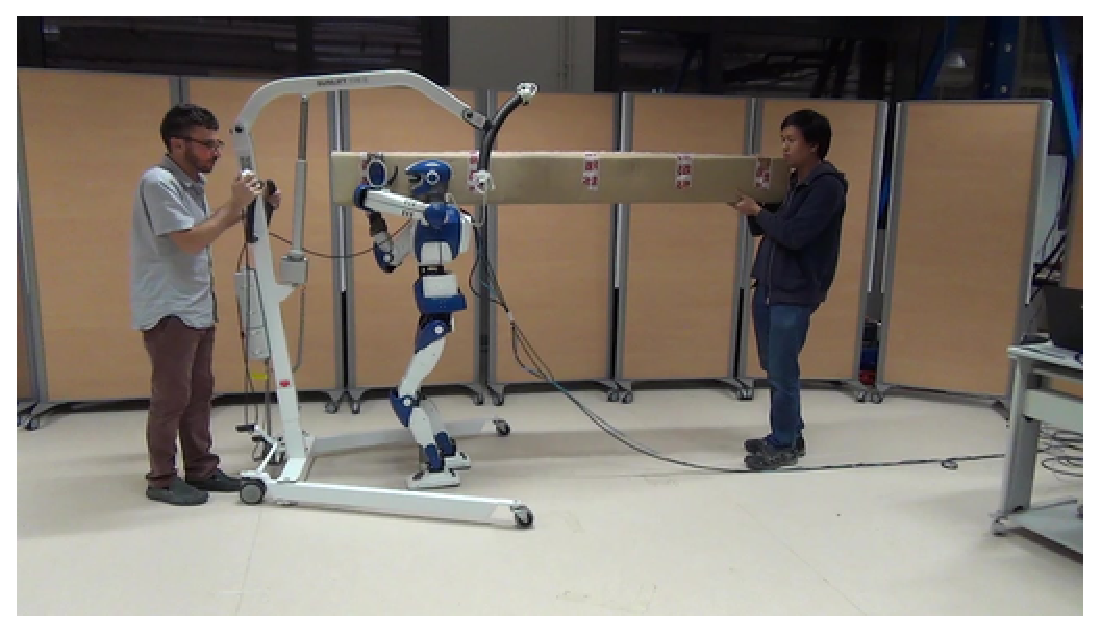
\includegraphics[scale=0.4]{collaboration_box4.eps}\\
            (3)
        }
    \end{minipage}
    \hfill
    \begin{minipage}[t]{0.49\textwidth}
        \centering{
            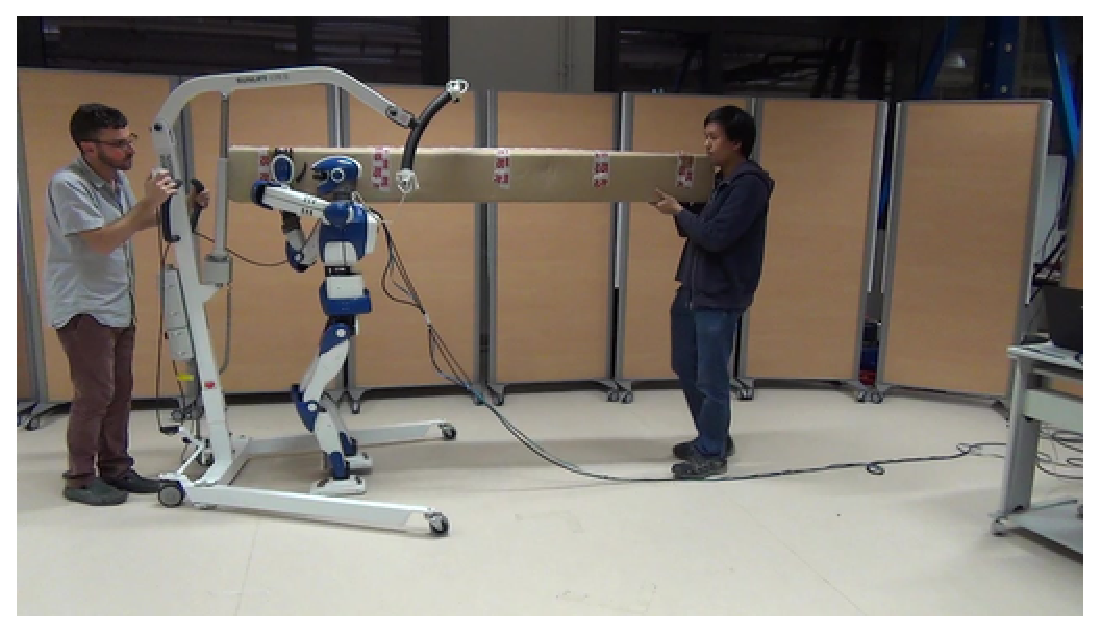
\includegraphics[scale=0.4]{collaboration_box5.eps}\\
            (4)
        }
    \end{minipage}
    \caption[Carrying a box in collaboration with a human.]{
        An \sn{HRP-4} \cite{Kaneko2011iros} carries a box in collaboration with
        a human.
    }
    \label{fig.collaboration_box}
\end{figure}


\begin{figure}[!htb]
    \begin{minipage}[t]{0.49\textwidth}
        \centering{
            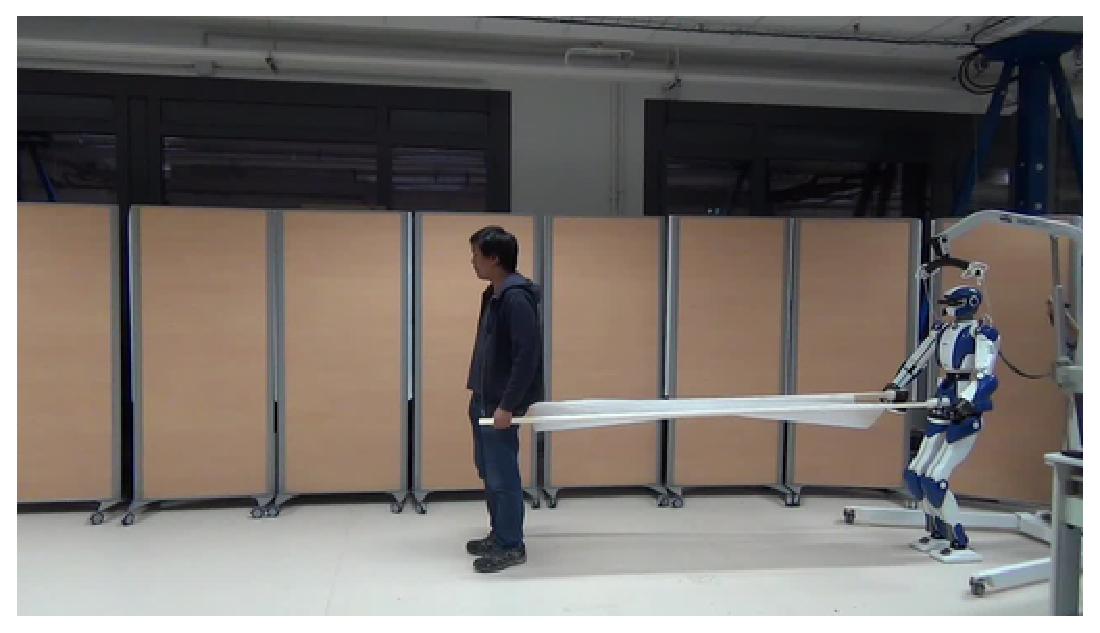
\includegraphics[scale=0.4]{collaboration_stretcher1.eps}\\
            (1)
            \vspace{0.2cm}
        }
    \end{minipage}
    \hfill
    \begin{minipage}[t]{0.49\textwidth}
        \centering{
            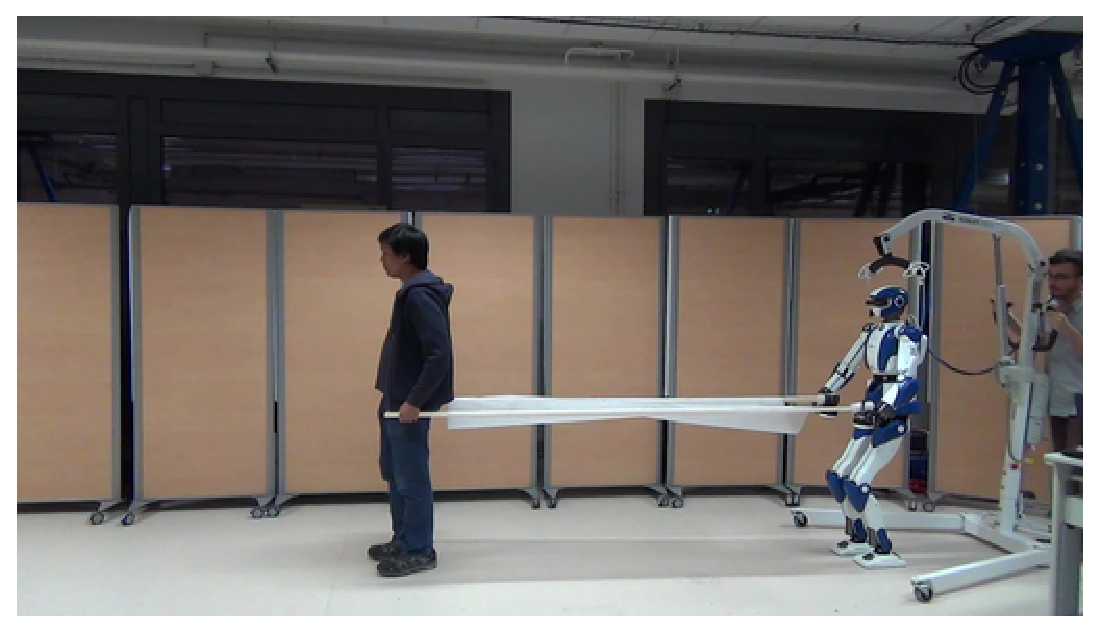
\includegraphics[scale=0.4]{collaboration_stretcher3.eps}\\
            (2)
            \vspace{0.2cm}
        }
    \end{minipage}
    \begin{minipage}[t]{0.49\textwidth}
        \centering{
            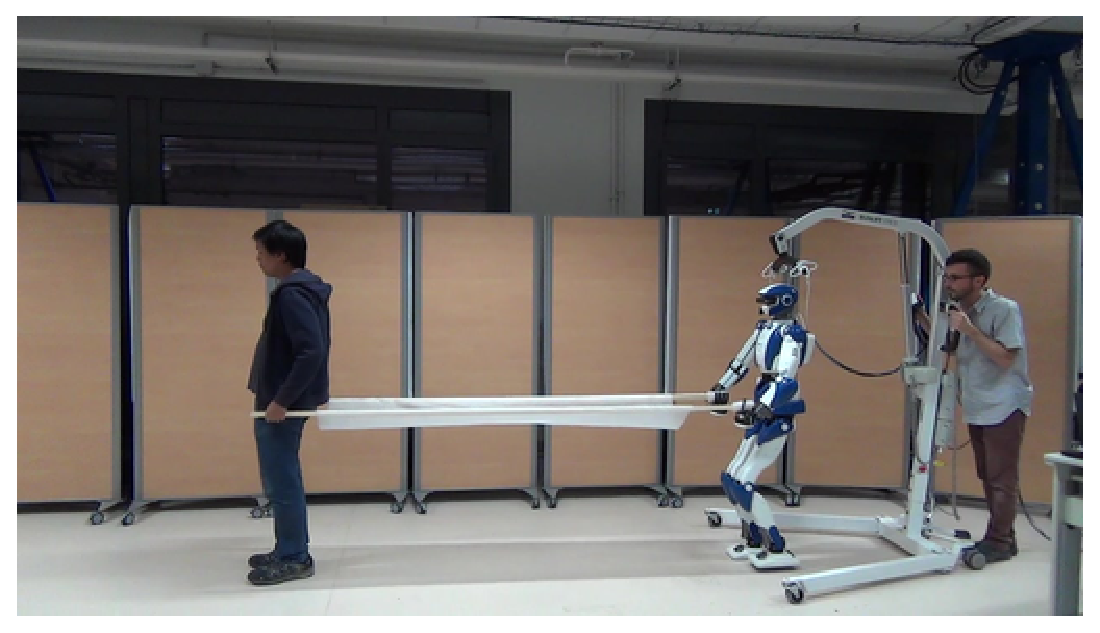
\includegraphics[scale=0.4]{collaboration_stretcher5.eps}\\
            (3)
        }
    \end{minipage}
    \hfill
    \begin{minipage}[t]{0.49\textwidth}
        \centering{
            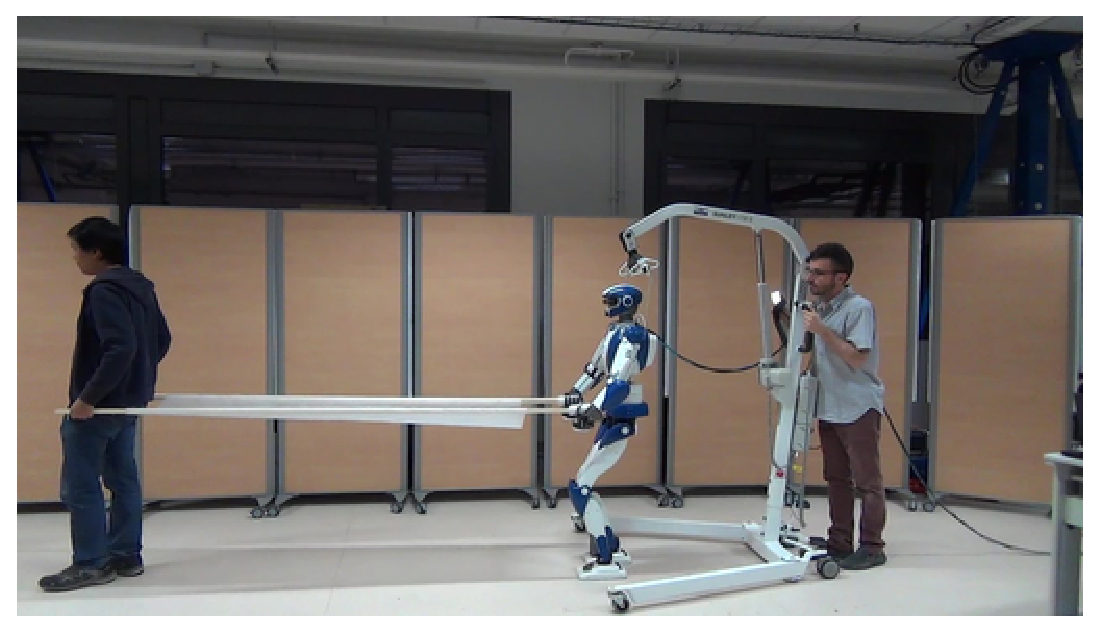
\includegraphics[scale=0.4]{collaboration_stretcher7.eps}\\
            (4)
        }
    \end{minipage}
    \caption[Carrying a stretcher in collaboration with a human.]{
        An \sn{HRP-4} \cite{Kaneko2011iros} carries a stretcher in
        collaboration with a human.
    }
    \label{fig.collaboration_stretcher}
\end{figure}

%-------------------------------------------------------------------------------
\chapter{Conclusion}
\label{ch.conclusion}
\acresetall
%-------------------------------------------------------------------------------

%%%%%%%%%%%%%%%%%%%%%%%%%%%%%%%%%%%%%%%%%%%%%%%%%%%%%%%%%%%%%%%%%%%%%%%%%%%%%%%%
%%%%%%%%%%%%%%%%%%%%%%%%%%%%%%%%%%%%%%%%%%%%%%%%%%%%%%%%%%%%%%%%%%%%%%%%%%%%%%%%
%%%%%%%%%%%%%%%%%%%%%%%%%%%%%%%%%%%%%%%%%%%%%%%%%%%%%%%%%%%%%%%%%%%%%%%%%%%%%%%%
\section{Summary}

This thesis aims at understanding and developing motion control of humanoid
robots, with an ultimate goal to make motion capabilities of humans and robots
comparable. One of the key aspects of human motion is preservation of balance.
An abstract discussion in \cref{ch.balance} led us to the conclusion that
preservation of balance is equivalent to maintaining capturability, \IE, the
ability to stop. The most practical way to ensure capturability is to
anticipate motions which are constrained to end in statically balanced states.
In order to account for non-deterministic changes in the environment,
anticipation must be performed in real time, which makes anticipation of whole
body motions a particularly challenging problem. A common approach is to
sacrifice quality and completeness of anticipated motions by employing
approximate models of humanoid robots. Approximate models lack the
expressiveness of whole body models (\cref{ch.modeling}) and, hence, cannot
accurately reflect whole body tasks and constraints. We address this drawback
by the integration of an instantaneous whole body motion controller with
anticipation based on an approximate model. We call this approach \ac{MMPC},
since we mix models of different accuracy within a single predictive controller
(\cref{ch.mpc}). While this idea applies to all kinds of models, we limit the
present work to linear models, which allows us to formulate our \ac{MMPC}
controllers as \ac{PLLS} optimization problems (\cref{ch.optimization}). We
evaluate our approach in simulations using two different \ac{MMPC} controllers
(\cref{ch.simulations}). One of them is capable of adjusting steps in response
to disturbances and under the influence of whole body tasks. The second one
includes a strict prioritization of the objectives in the controller in order
to exploit additional hand contact with the environment only when it is
necessary for balance preservation or execution of a particular whole body
task. The results obtained with both controllers support the validity of our
approach. There is, of course, a number of topics for further investigation in
the considered controllers, in \ac{MMPC}, modeling of humanoid robots, and
solution of \ac{PLLS} problems. We give a brief outlook of these topics in the
following section.



%%%%%%%%%%%%%%%%%%%%%%%%%%%%%%%%%%%%%%%%%%%%%%%%%%%%%%%%%%%%%%%%%%%%%%%%%%%%%%%%
%%%%%%%%%%%%%%%%%%%%%%%%%%%%%%%%%%%%%%%%%%%%%%%%%%%%%%%%%%%%%%%%%%%%%%%%%%%%%%%%
%%%%%%%%%%%%%%%%%%%%%%%%%%%%%%%%%%%%%%%%%%%%%%%%%%%%%%%%%%%%%%%%%%%%%%%%%%%%%%%%
\section{Perspectives}

%%%%%%%%%%%%%%%%%%%%%%%%%%%%%%%%%%%%%%%%%%%%%%%%%%%%%%%%%%%%%%%%%%%%%%%%%%%%%%%%
\subsection{Mixed Model Predictive Control}

It appears that the discrepancy between the whole body motion control sampling
time and the anticipation sampling time results in periodic variations in
commands generated by \ac{MMPC} controllers. We discuss this issue in
\cref{sec.sampling_interval,sec.motion_quality,sec.force_results}, but so far
could not propose a satisfactory solution. Therefore, it is an important topic
for further research.


%%%%%%%%%%%%%%%%%%%%%%%%%%%%%%%%%%%%%%%%%%%%%%%%%%%%%%%%%%%%%%%%%%%%%%%%%%%%%%%%
\subsection{Walking using an approximate model}

The \ac{MMPC} controller for walking considered in \cref{sec.task_walk}
requires further development to make it interesting for practical applications.
Though such limitations as fixed duration and sequence of steps are unlikely to
be lifted without adoption of nonlinear approximate models, there is still room
for improvement with linear models:
%
\begin{itemize}
    \item It is possible to enable walking with varying \ac{CoM} height using
        the recent proposal from \cite{Brasseur2015humanoids}.

    \item We can abandon the point-mass model and employ a model including
        angular momentum. Incorporation of angular momentum in the
        capturability constraint may help to avoid situations when the
        currently used capturability constraint is not sufficient for
        preservation of balance (see \cref{sec.walk_capturability}).
        Furthermore, angular momentum allows to account for motions of heavy
        end-effectors, \EG, legs, in the anticipated motions (see
        \cref{sec.approx_models_limitations}).

    \item So far we used simple cubic polynomials for generation of foot
        trajectories. Instead, we can adopt a triple integrator for this
        purpose, in the same way as we do for the \ac{CoM} motion in
        \nameref{model.CPPMJ} model. This modification introduces additional
        freedom in trajectory generation and allows for variation of the step
        height or simple obstacle avoidance.

    \item In this work we did not realize rotations of the robot and its feet,
        which is a significant drawback. In general, rotations result in
        nonlinear constraints on the \ac{CoP} positions and positions of the
        feet. We can address the first problem by shrinking the \ac{CoP}
        constraints as proposed in \cref{sec.surface_contacts}. The second
        problem can be avoided by reducing the length of the preview horizon
        from $2$ to $1$ step, which we have already demonstrated to be possible
        in \cref{sec.walk_performance}.
\end{itemize}
%
Last, but not least is the experimental evaluation of the controller on a real
robot.


%%%%%%%%%%%%%%%%%%%%%%%%%%%%%%%%%%%%%%%%%%%%%%%%%%%%%%%%%%%%%%%%%%%%%%%%%%%%%%%%
\subsection{Prioritization in contact force distribution}

Further development of the idea of prioritization in contact force distribution
for partial contact planning as explained in \cref{sec.force_conclusion} is
appealing, but may require significant improvements in numerical tools to make
it applicable in practice.


%%%%%%%%%%%%%%%%%%%%%%%%%%%%%%%%%%%%%%%%%%%%%%%%%%%%%%%%%%%%%%%%%%%%%%%%%%%%%%%%
\subsection{Solvers for optimization problems with prioritization}

We see two primary directions for improvement of the existing solvers of
\acf{PLLS} problems:
%
\begin{itemize}
    \item We would like the solvers to be able to exploit general sparsity
        patterns in the objectives for improvement of performance and not only
        simple bounds. Ideally, we would like to avoid any manual variable
        elimination steps before solution of a \ac{PLLS} problem.

    \item The current mechanisms for coping with issues near singularities
        appear to be insufficient and require further development (see
        \cref{sec.force_conclusion}).
\end{itemize}


%---------------------------------------
% Appendix
%---------------------------------------
\appendix
%-------------------------------------------------------------------------------
\chapter{Dynamics of a multibody system}
\label{app.dynamics}
\acresetall
%-------------------------------------------------------------------------------

In this appendix we derive equation of dynamics of a floating base multibody
system with unilateral constraints. The presentation is based on
\cite{Wieber2006fastmotions}, and likewise aims at exposing the structure of
this equation, rather than at fast computation of its components. In addition
to that, we demonstrate how momenta of the whole system are computed.



%%%%%%%%%%%%%%%%%%%%%%%%%%%%%%%%%%%%%%%%%%%%%%%%%%%%%%%%%%%%%%%%%%%%%%%%%%%%%%%%
%%%%%%%%%%%%%%%%%%%%%%%%%%%%%%%%%%%%%%%%%%%%%%%%%%%%%%%%%%%%%%%%%%%%%%%%%%%%%%%%
%%%%%%%%%%%%%%%%%%%%%%%%%%%%%%%%%%%%%%%%%%%%%%%%%%%%%%%%%%%%%%%%%%%%%%%%%%%%%%%%
\section{Preliminaries}

%%%%%%%%%%%%%%%%%%%%%%%%%%%%%%%%%%%%%%%%%%%%%%%%%%%%%%%%%%%%%%%%%%%%%%%%%%%%%%%%
\subsection{Notation}

We consider a system of $n + 1$ interconnected rigid bodies. We associate the
following variables with each body $k \in \{1, ..., n+1\}$
%
\begin{longtable}[l]{@{\extracolsep{0pt}}l @{\extracolsep{3pt}}l p{9.5cm}}
    $m_k$                                           & $\in \RR_{>0}$                 & mass of $k$-th body\\
    $\V{c}_k$                                       & $\in \RR^3$                   & position of \ac{CoM} of $k$-th body in the global frame\\
    $\ddotV{x}_k = (\ddotV{c}_k, \dotV{\omega}_k)$  & $\in \RR^6$                   & constrained spatial acceleration of $k$-th body in frame $\FRAME{k}$\\
    $\ddotV{x}_{k,u}$                               & $\in \RR^6$                   & unconstrained spatial acceleration of $k$-th body in frame $\FRAME{k}$\\
    $\INERTIA_k$                                    & $\in \RR^{3 \CROSS 3}$        & inertia matrix of $k$-th body in frame $\FRAME{k}$\\
    $\M{H}_k = \begin{bmatrix}
                    m_k \V{I}_3 & \V{0}      \\
                    \V{0}       & \INERTIA_k
               \end{bmatrix}$                       & $\in \RR^{6 \CROSS 6}$        & spatial inertia matrix of $k$-th body in frame $\FRAME{k}$\\
    $(\V{f}_k, \moment_k)$                          & $\in \RR^{6 \CROSS 6}$        & wrench acting on $k$-th body in frame $\FRAME{k}$\\
    $\M{J}_k = (\M{J}_{\TRAN,k}, \M{J}_{\ROT,k})$   & $\in \RR^{6 \CROSS (n+6)}$      & Jacobian of $k$-th body\\
\end{longtable}
%
\noindent and fix frame $\FRAME{k}$ to the \ac{CoM} of $k$-th body. All frames
$\FRAME{k}$, as well as frame $\FRAME{r}$ fixed to the base have the same
orientation as the global frame. Also, we reuse some of the variables defined
in \cref{sec.complementarity_system}
%
\begin{longtable}[l]{@{\extracolsep{0pt}}l @{\extracolsep{3pt}}l p{9.5cm}}
    $\q = (\qn, \V{r}, \V{\EULER})$         & $\in \RR^{n+6}$             & vector of generalized coordinates\\
    $\M{H}(\q)$                             & $\in \RR^{(n+6) \CROSS (n+6)}$    & inertia matrix of the whole system\\
    $\V{h}(\q, \dq)$                        & $\in \RR^{n+6}$               & vector of Coriolis and centrifugal terms of the whole system\\
    $\Jcom$                                 & $\in \RR^{3 \CROSS (n+6)}$      & Jacobian of the \ac{CoM}\\
    $\Itorques$                             & $\in \RR^{(n+6) \CROSS n}$      & torque selection matrix\\
    $\V{g}$                                 & $\in \RR^3$                   & vector of gravitational acceleration\\
    $m$                                     & $\in \RR_{>0}$                 & total mass of the system\\
\end{longtable}
%


%%%%%%%%%%%%%%%%%%%%%%%%%%%%%%%%%%%%%%%%%%%%%%%%%%%%%%%%%%%%%%%%%%%%%%%%%%%%%%%%
\subsection{Structure of Jacobians}\label{sec.jacobians}

Vector of generalized coordinates $\V{q}$ contains three parts corresponding to
joint angles, position, and orientation of the base. Consequently, the Jacobians,
which map generalized velocities to the twist of the $k$-th body
%
\begin{equation}
    \begin{bmatrix}
        \dotV{c}_k \\
        \V{\omega}_k
    \end{bmatrix}
    =
    \begin{bmatrix}
        \M{J}_{\TRAN,k}\\
        \M{J}_{\ROT,k}\\
    \end{bmatrix}
    \dq
    =
    \M{J}_k
    \dq
    ,
\end{equation}
%
have corresponding structure:
%
\begin{equation}
    \M{J}_k
    =
    \begin{bmatrix}
        \M{J}_{\TRAN,k}\\
        \M{J}_{\ROT,k}\\
    \end{bmatrix}
    =
    \begin{bmatrix}
        \M{J}_{\TRAN,k,1}  &  \M{J}_{\TRAN,k,2}  &  \M{J}_{\TRAN,k,3}\\
        \M{J}_{\ROT,k,1}  &  \M{J}_{\ROT,k,2}  &  \M{J}_{\ROT,k,3}\\
    \end{bmatrix}
    =
    \begin{bmatrix}
        \M{J}_{\TRAN,k,1}  &  \M{I}_3  &  - \CROSS[(\V{c}_k - \V{r})] \\
        \M{J}_{\ROT,k,1}  &  \M{0}_{3,3}  &  \M{I}_3\\
    \end{bmatrix}
\end{equation}
%


In situations when orientation of the base is represented by Euler angles
$\V{\EULER} \in \RR^3$ and its angular velocity and acceleration are replaced
with $\dotV{\EULER}$ and $\ddotV{\EULER}$, it is necessary to introduce matrix
$\Teuler$, which transforms derivatives of the Euler angles to angular
velocities:
%
\begin{equation}
    \M{J}_k
    =
    \begin{bmatrix}
        \M{J}_{\TRAN,k,1}  &  \M{I}_3  &  - \CROSS[(\V{c}_k - \V{r})] \Teuler\\
        \M{J}_{\ROT,k,1}  &  \M{0}_{3,3}  &  \Teuler\\
    \end{bmatrix}
    =
    \begin{bmatrix}
        \M{J}_{\TRAN,k,1}  &  \M{I}_3  &  \T{(\CROSS[(\V{c}_k - \V{r})])} \Teuler\\
        \M{J}_{\ROT,k,1}  &  \M{0}_{3,3}  &  \Teuler\\
    \end{bmatrix}
\end{equation}
%
Henceforth, we use this version of the Jacobian, since we represent
orientation, angular velocity and acceleration of the base using Euler angles
in our simulations.


%%%%%%%%%%%%%%%%%%%%%%%%%%%%%%%%%%%%%%%%%%%%%%%%%%%%%%%%%%%%%%%%%%%%%%%%%%%%%%%%
%%%%%%%%%%%%%%%%%%%%%%%%%%%%%%%%%%%%%%%%%%%%%%%%%%%%%%%%%%%%%%%%%%%%%%%%%%%%%%%%
%%%%%%%%%%%%%%%%%%%%%%%%%%%%%%%%%%%%%%%%%%%%%%%%%%%%%%%%%%%%%%%%%%%%%%%%%%%%%%%%
\section{Gauss' principle}

The Gauss' principle states that constrained motions of rigid bodies in a
system are as close as possible to the unconstrained motions in least-squares
sense \cite{Wieber2006fastmotions, Moreau1966siamjc}. Based on this principle
we define the following optimization problem:
%
\begin{equation}
    \begin{aligned}
            \MINIMIZE{\ddotV{x}_1, \dots, \ddotV{x}_n, \ddot{q}}
                        & \frac{1}{2} \sum_{k=1}^{n+1}
                            \T{(\ddotV{x}_k - \ddotV{x}_{k,u})}
                            \M{H}_k
                            (\ddotV{x}_k - \ddotV{x}_{k,u}) \\
            \SUBJECTTO  & \ddotV{x}_k =
                            \begin{bmatrix}
                                \ddotV{c}_k\\
                                \dotV{\omega}_k\\
                            \end{bmatrix}
                            =
                            \begin{bmatrix}
                                \M{J}_{\TRAN,k}\\
                                \M{J}_{\ROT,k}\\
                            \end{bmatrix}
                            \ddotV{q}
                            +
                            \begin{bmatrix}
                                \dotM{J}_{\TRAN,k}\\
                                \dotM{J}_{\ROT,k}\\
                            \end{bmatrix}
                            \dotV{q}
                            =
                            \M{J}_k \ddotV{q} + \dotM{J}_k \dotV{q} \\
                        & \M{H}_k \ddotV{x}_{k,u} =
                            \begin{bmatrix}
                                \V{f}_k\\
                                \moment_k - \V{\omega}_k \CROSS \INERTIA_k \V{\omega}_k \\
                            \end{bmatrix}\\
                        & \ddotV{c}_j =
                            \M{J}_{\TRAN,j}
                            \ddotV{q}
                            +
                            \dotM{J}_{\TRAN,j}
                            \dotV{q}
                            \ge
                            \V{b}_j,
    \end{aligned}
\end{equation}
%
where inequality constraint on $\ddotV{c}_j$ with $j \in \{1, ..., n+1\}$ is
added for illustration. Handling of this constraint is easily generalized to
arbitrary inequalities, such as contact constraints in
\cref{sec.whole_body_model}.


First, we expand multiplication in the objective function and eliminate
constant terms to obtain:
%
\begin{equation}
    \begin{aligned}
            \MINIMIZE{\ddotV{x}_1, \dots, \ddotV{x}_n, \ddot{q}}
                        & \frac{1}{2} \sum_{k=1}^{n+1}
                            \left(
                                \T{\ddotV{x}_k}  \M{H}_k  \ddotV{x}_k
                                -
                                2 \T{\ddotV{x}_k}  \M{H}_k  \ddotV{x}_{k,u}
                            \right)\\
            \SUBJECTTO  & \ddotV{x}_k =
                            \M{J}_k \ddotV{q} + \dotM{J}_k \dotV{q} \\
                        & \M{H}_k \ddotV{x}_{k,u} =
                            \begin{bmatrix}
                                \V{f}_k\\
                                \moment_k - \V{\omega}_k \CROSS \INERTIA_k \V{\omega}_k \\
                            \end{bmatrix}\\
                        &   \M{J}_{\TRAN,j}
                            \ddotV{q}
                            +
                            \dotM{J}_{\TRAN,j}
                            \dotV{q}
                            \ge
                            \V{b}_j.
    \end{aligned}
\end{equation}
%
Then we eliminate all equality constraints
%
\begin{equation}
    \begin{aligned}
            \MINIMIZE{\ddot{q}}
                        & \frac{1}{2} \sum_{k=1}^{n+1}
                            \Bigg(
                            \T{(\M{J}_k \ddotV{q})}  \M{H}_k  \M{J}_k \ddotV{q}
                            +
                            2 \T{(\M{J}_k \ddotV{q})}  \M{H}_k  \dotM{J}_k \dotV{q}
                            +
                            \T{(\dotM{J}_k \dotV{q})}  \M{H}_k  \dotM{J}_k \dotV{q}\\
                        &
                            -
                            2 \T{(\M{J}_k \ddotV{q} + \dotM{J}_k \dotV{q})}
                            \begin{bmatrix}
                                \V{f}_k\\
                                \moment_k - \V{\omega}_k \CROSS \INERTIA_k \V{\omega}_k \\
                            \end{bmatrix} \Bigg)\\
            \SUBJECTTO  &   \M{J}_{\TRAN,j}
                            \ddotV{q}
                            +
                            \dotM{J}_{\TRAN,j}
                            \dotV{q}
                            \ge
                            \V{b}_j,
    \end{aligned}
\end{equation}
%
and drop the constant terms
%
\begin{equation}
    \begin{aligned}
            \MINIMIZE{\ddot{q}}
                        & \sum_{k=1}^{n+1}
                            \left(
                            \frac{1}{2} \T{(\M{J}_k \ddotV{q})}  \M{H}_k  \M{J}_k \ddotV{q}
                            +
                            \T{(\M{J}_k \ddotV{q})}  \M{H}_k  \dotM{J}_k \dotV{q}
                            -
                            \T{(\M{J}_k \ddotV{q})}
                            \begin{bmatrix}
                                \V{f}_k\\
                                \moment_k - \V{\omega}_k \CROSS \INERTIA_k \V{\omega}_k \\
                            \end{bmatrix}
                            \right)\\
            \SUBJECTTO  &   \M{J}_{\TRAN,j}
                            \ddotV{q}
                            +
                            \dotM{J}_{\TRAN,j}
                            \dotV{q}
                            \ge
                            \V{b}
    \end{aligned}
\end{equation}
%


\ac{KKT} optimality conditions for the considered problem are stated as a
complementarity system \cite{Nocedal2006numopt}
\begin{subequations}\label{eq.kkt_dynamics}
\begin{empheq}[left=\empheqlbrace]{align}
    &   \sum_{k=1}^{n+1}
        \left(
            \T{\M{J}_k}  \M{H}_k  \M{J}_k \ddotV{q}
            +
            \T{\M{J}_k}  \M{H}_k  \dotM{J}_k \dotV{q}
            -
            \T{\M{J}_k}
            \begin{bmatrix}
                \V{f}_k\\
                \moment_k - \V{\omega}_k \CROSS \INERTIA_k \V{\omega}_k \\
            \end{bmatrix}
        \right)
        -
        \T{\M{J}_{\TRAN,j}}
        \V{\Lambda}
        = 0, \label{eq.kkt_dynamics.dynamics}\\
    &   \M{J}_{\TRAN,j}
        \ddotV{q}
        +
        \dotM{J}_{\TRAN,j}
        \dotV{q}
        \ge
        \V{b},\\
    &   \V{\Lambda} \ge \V{0},\\
    &   \T{\V{\Lambda}}
        \left(
            \M{J}_{\TRAN,j}
            \ddotV{q}
            +
            \dotM{J}_{\TRAN,j}
            \dotV{q}
            -
            \V{b}
        \right)
        =
        \V{0},
\end{empheq}
\end{subequations}
where $\V{\Lambda}$ is the vector of Lagrange multipliers.
System~\cref{eq.kkt_dynamics} corresponds to the complementarity system
presented in \cref{sec.whole_body_model}: the first line is the equation of
dynamics of the whole system and $\V{\Lambda}$ correspond to the contact
forces.


We further modify \cref{eq.kkt_dynamics.dynamics} by substituting
$\V{\omega}_k = \M{J}_{\ROT,k} \dotV{q}$ and moving all forces to the right
side:
%
\begin{equation}\label{eq.lagrangian_dynamics}
    \underbrace{
        \sum_{k=1}^{n+1}
        \left(
            \T{\M{J}_k}  \M{H}_k  \M{J}_k
        \right)
    }_{\M{H}}
    \ddotV{q}
    +
    \underbrace{
        \sum_{k=1}^{n+1}
        \left(
            \T{\M{J}_k}  \M{H}_k  \dotM{J}_k \dotV{q}\\
            +
            \T{\M{J}_{\ROT,k}}
            ((\M{J}_{\ROT,k} \dotV{q}) \CROSS \INERTIA_k \M{J}_{\ROT,k} \dotV{q})
        \right)
    }_{\V{h}}
    =
    \sum_{k=1}^{n+1}
    \T{\M{J}_k}
    \begin{bmatrix}
        \V{f}_k\\
        \moment_k\\
    \end{bmatrix}
    +
    \T{\M{J}_{\TRAN,j}}
    \V{\Lambda}.
\end{equation}
%


%%%%%%%%%%%%%%%%%%%%%%%%%%%%%%%%%%%%%%%%%%%%%%%%%%%%%%%%%%%%%%%%%%%%%%%%%%%%%%%%
%%%%%%%%%%%%%%%%%%%%%%%%%%%%%%%%%%%%%%%%%%%%%%%%%%%%%%%%%%%%%%%%%%%%%%%%%%%%%%%%
%%%%%%%%%%%%%%%%%%%%%%%%%%%%%%%%%%%%%%%%%%%%%%%%%%%%%%%%%%%%%%%%%%%%%%%%%%%%%%%%
\section{Structure of the equation of dynamics}

In this section we employ our knowledge of the structure of Jacobians to
explore the structure of components of Equation~\cref{eq.lagrangian_dynamics}.


%%%%%%%%%%%%%%%%%%%%%%%%%%%%%%%%%%%%%%%%%%%%%%%%%%%%%%%%%%%%%%%%%%%%%%%%%%%%%%%%
\subsection{Inertia matrix}

Expansion of the Jacobians exposes the structure of inertia matrix as shown
below
%
\begin{subequations}
\begin{align}
    \M{H}
    & =
    \sum_{k=1}^{n+1}
    \T{\M{J}_k}  \M{H}_k  \M{J}_k \\
    & =
    \sum_{k=1}^{n+1}
    m_k \T{\M{J}_{\TRAN,k}}  \M{J}_{\TRAN,k}
    +
    \sum_{k=1}^{n+1}
    \T{\M{J}_{\ROT,k}}  \INERTIA_k  \M{J}_{\ROT,k} \\
    & =
    \sum_{k=1}^{n+1}
    \left(
        m_k
        \begin{bmatrix}
            \T{\M{J}_{\TRAN,k,1}}  \M{J}_{\TRAN,k}\\
            \T{\M{J}_{\TRAN,k,2}}  \M{J}_{\TRAN,k}\\
            \T{\M{J}_{\TRAN,k,3}}  \M{J}_{\TRAN,k}\\
        \end{bmatrix}
        +
        \begin{bmatrix}
            \T{\M{J}_{\ROT,k,1}} \INERTIA_k \M{J}_{\ROT,k}\\
            \T{\M{J}_{\ROT,k,2}} \INERTIA_k \M{J}_{\ROT,k}\\
            \T{\M{J}_{\ROT,k,3}} \INERTIA_k \M{J}_{\ROT,k}\\
        \end{bmatrix}
    \right)\\
    \begin{split}
    &
    =
    \sum_{k=1}^{n+1}
    \Bigg(
        m_k
        \begin{bmatrix}
            \T{\M{J}_{\TRAN,k,1}}  \M{J}_{\TRAN,k,1}                    & \T{\M{J}_{\TRAN,k,1}}                 & - \T{\M{J}_{\TRAN,k,1}}  \CROSS[(\V{c}_k - \V{r})] \Teuler\\
            \M{J}_{\TRAN,k,1}                                           & \V{I}_3                               & - \CROSS[(\V{c}_k - \V{r})] \Teuler\\
            \T{\Teuler} \CROSS[(\V{c}_k - \V{r})]  \M{J}_{\TRAN,k,1}  & \T{\Teuler} \CROSS[(\V{c}_k - \V{r})] & - \T{\Teuler} \CROSS[(\V{c}_k - \V{r})] \CROSS[(\V{c}_k - \V{r})] \Teuler\\
        \end{bmatrix}\\
        & \quad \quad \quad \quad +
        \begin{bmatrix}
            \T{\M{J}_{\ROT,k,1}} \INERTIA_k \M{J}_{\ROT,k,1}    & \M{0}_{n,3} & \T{\M{J}_{\ROT,k,1}} \INERTIA_k \Teuler\\
            \M{0}_{3,n}                                         & \M{0}_{3,3} & \M{0}_{3,3}\\
            \T{\Teuler} \INERTIA_k \M{J}_{\ROT,k,1}             & \M{0}_{3,3} & \T{\Teuler} \INERTIA_k \Teuler\\
        \end{bmatrix}
    \Bigg)
    \end{split}
    \label{eq.inertia_structure.long_line}
    \\
    & =
    \sum_{k=1}^{n+1}
    \left(
        m_k
        \begin{bmatrix}
            \T{\M{J}_{\TRAN,k,1}}  \M{J}_{\TRAN,k}\\
            \M{J}_{\TRAN,k}                     \\
            \T{\Teuler} \CROSS[(\V{c}_k - \V{r})] \M{J}_{\TRAN,k}\\
        \end{bmatrix}
        +
        \begin{bmatrix}
            \T{\M{J}_{\ROT,k,1}} \INERTIA_k \M{J}_{\ROT,k}\\
            \M{0}_{n+6,3}                                              \\
            \T{\Teuler} \INERTIA_k \M{J}_{\ROT,k}\\
        \end{bmatrix}
    \right)
    =
    \begin{bmatrix}
        \M{H}_{1} \\
        \M{H}_{2} \\
        \M{H}_{3} \\
    \end{bmatrix}
\end{align}
\end{subequations}
%

It is worth noting that the structure of the inertia matrix simplifies when the
base $\V{r}$ is chosen to coincide with the \ac{CoM} $\V{c}$. In this case some
of the components of $\M{H}$ are equal to zero due to
%
\begin{equation}
    \sum_{k=1}^{n+1}
        m_k \CROSS[(\V{c}_k - \V{r})]
    =
    \sum_{k=1}^{n+1}
        \CROSS[(m_k \V{c}_k - m_k \V{c})]
    =
    \CROSS[\left(m \V{c} - \sum_{k=1}^{n+1} (m_k \V{c})\right)]
    =
    \CROSS[(\M{0}_{3,1})]
    =
    \M{0}_{3,3}.
\end{equation}
%


%%%%%%%%%%%%%%%%%%%%%%%%%%%%%%%%%%%%%%%%%%%%%%%%%%%%%%%%%%%%%%%%%%%%%%%%%%%%%%%%
\subsection{Nonlinear term}
%
\begin{equation}
\begin{aligned}
    &\V{h}
     =
    \sum_{k=1}^{n+1}
    \left(
        \M{J}_k^T  \M{H}_k  \dotM{J}_k \dotV{q}
        +
        \M{J}_{\ROT,k}^T
        ((\M{J}_{\ROT,k} \dotV{q}) \CROSS \INERTIA_k \M{J}_{\ROT,k} \dotV{q})
    \right)\\
    & =
    \sum_{k=1}^{n+1}
    \left(
        m_k
        \begin{bmatrix}
            \M{J}_{\TRAN,k,1}^T  \dotM{J}_{\TRAN,k} \dotV{q}\\
            \dotM{J}_{\TRAN,k} \dotV{q}                     \\
            \T{\Teuler} \CROSS[(\V{c}_k - \V{r})] \dotM{J}_{\TRAN,k} \dotV{q}\\
        \end{bmatrix}
        +
        \begin{bmatrix}
            \M{J}_{\ROT,k,1}^T \INERTIA_k \dotM{J}_{\ROT,k} \dotV{q} + \M{J}_{\ROT,k,1}^T ((\M{J}_{\ROT,k} \dotV{q}) \CROSS \INERTIA_k \M{J}_{\ROT,k} \dotV{q})\\
            \M{0}_{3,1} \\
            \T{\Teuler} \INERTIA_k \dotM{J}_{\ROT,k} \dotV{q}        + \T{\Teuler} ((\M{J}_{\ROT,k} \dotV{q}) \CROSS \INERTIA_k \M{J}_{\ROT,k} \dotV{q})\\
        \end{bmatrix}
    \right)
    \\
    & =
    \begin{bmatrix}
        \M{h}_{1} \\
        \M{h}_{2} \\
        \M{h}_{3} \\
    \end{bmatrix}
\end{aligned}
\end{equation}
%


%%%%%%%%%%%%%%%%%%%%%%%%%%%%%%%%%%%%%%%%%%%%%%%%%%%%%%%%%%%%%%%%%%%%%%%%%%%%%%%%
\subsection{Forces}

Assuming that the wrenches $(\V{f}_k, \moment_k)$ are the result of gravity
field and joint torques we obtain
%
\begin{equation}
    \sum_{k=1}^{n+1}
    \T{\M{J}_k}
    \begin{bmatrix}
        \V{f}_k\\
        \moment_k\\
    \end{bmatrix}
    +
    \T{\M{J}_{\TRAN,j}}
    \V{\Lambda}
    =
    \sum_{k=1}^{n+1}
    \left(
        m_k
        \begin{bmatrix}
            \M{J}_{\TRAN,k,1}^T\\
            \M{I}_3                     \\
            \T{\Teuler} \CROSS[(\V{c}_k - \V{r})]\\
        \end{bmatrix}
    \right)
    \V{g}
    +
    \Itorques
    \torques
    +
    \begin{bmatrix}
        \M{J}_{\TRAN,j,1}^T\\
        \M{I}_3                     \\
        \T{\Teuler} \CROSS[(\V{c}_j - \V{r})]\\
    \end{bmatrix}
    \V{\Lambda}.
\end{equation}
%



%%%%%%%%%%%%%%%%%%%%%%%%%%%%%%%%%%%%%%%%%%%%%%%%%%%%%%%%%%%%%%%%%%%%%%%%%%%%%%%%
%%%%%%%%%%%%%%%%%%%%%%%%%%%%%%%%%%%%%%%%%%%%%%%%%%%%%%%%%%%%%%%%%%%%%%%%%%%%%%%%
%%%%%%%%%%%%%%%%%%%%%%%%%%%%%%%%%%%%%%%%%%%%%%%%%%%%%%%%%%%%%%%%%%%%%%%%%%%%%%%%
\section{Momenta of the system}\label{sec.momenta_structure}

Consider the lower $6$ lines of the equation of dynamics:
%
\begin{equation}
\begin{aligned}
    &
    \begin{bmatrix}
        \M{I}_3   &   \M{0}_{3,3} \\
        \M{0}_{3,3}   &   \T{\Teuler}\\
    \end{bmatrix}
    \Bigg(
        \sum_{k=1}^{n+1}
        \left(
            m_k
            \begin{bmatrix}
                \M{J}_{\TRAN,k}                     \\
                \CROSS[(\V{c}_k - \V{r})] \M{J}_{\TRAN,k}\\
            \end{bmatrix}
            +
            \begin{bmatrix}
                \M{0}_{3,n+6}                                              \\
                \INERTIA_k \M{J}_{\ROT,k}\\
            \end{bmatrix}
        \right)
        \ddotV{q}
        \\
        &+
        \sum_{k=1}^{n+1}
        \left(
            m_k
            \begin{bmatrix}
                \dotM{J}_{\TRAN,k} \dotV{q}                     \\
                \CROSS[(\V{c}_k - \V{r})] \dotM{J}_{\TRAN,k} \dotV{q}\\
            \end{bmatrix}
            +
            \begin{bmatrix}
                \M{0}_{3,1}                                              \\
                \INERTIA_k \dotM{J}_{\ROT,k} \dotV{q}\\
            \end{bmatrix}
            +
            \begin{bmatrix}
                \M{0}_{3,1}                                          \\
                ((\M{J}_{\ROT,k} \dotV{q}) \CROSS \INERTIA_k \M{J}_{\ROT,k} \dotV{q})\\
            \end{bmatrix}
        \right)
    \Bigg)
    \\
    & =
    \begin{bmatrix}
        \M{I}_3   &   \M{0}_{3,3} \\
        \M{0}_{3,3}   &   \T{\Teuler}\\
    \end{bmatrix}
    \Bigg(
        \sum_{k=1}^{n+1}
        \left(
            m_k
            \begin{bmatrix}
                \M{I}_3                     \\
                \CROSS[(\V{c}_k - \V{r})]\\
            \end{bmatrix}
        \right)
        \V{g}
        +
        \begin{bmatrix}
            \M{I}_3                     \\
            \CROSS[(\V{c}_j - \V{r})]\\
        \end{bmatrix}
        \V{\Lambda}
    \Bigg)
    .
\end{aligned}
\end{equation}
%
%
This is the Newton-Euler equation of the whole system multiplied by the
constant matrix $\diag{}{\M{I}_3, \T{\Teuler}}$ \cite{Wieber2006fastmotions}.
The right hand side of the equation gives the total wrench acting at the
reference point $\V{r}$ of the system, hence
%
\begin{equation}
\begin{aligned}
    &\sum_{k=1}^{n+1}
    \left(
        m_k
        \begin{bmatrix}
            \M{J}_{\TRAN,k}                     \\
            \CROSS[(\V{c}_k - \V{r})] \M{J}_{\TRAN,k}\\
        \end{bmatrix}
        +
        \begin{bmatrix}
            \M{0}_{3,n+6}                                              \\
            \INERTIA_k \M{J}_{\ROT,k}\\
        \end{bmatrix}
    \right)
    \ddotV{q}
    \\
    &+
    \sum_{k=1}^{n+1}
    \left(
        m_k
        \begin{bmatrix}
            \dotM{J}_{\TRAN,k} \dotV{q}                     \\
            \CROSS[(\V{c}_k - \V{r})] \dotM{J}_{\TRAN,k} \dotV{q}\\
        \end{bmatrix}
        +
        \begin{bmatrix}
            \M{0}_{3,1}                                              \\
            \INERTIA_k \dotM{J}_{\ROT,k} \dotV{q}\\
        \end{bmatrix}
        +
        \begin{bmatrix}
            \M{0}_{3,1}                                              \\
            ((\M{J}_{\ROT,k} \dotV{q}) \CROSS \INERTIA_k \M{J}_{\ROT,k} \dotV{q})\\
        \end{bmatrix}
    \right)
    \\
    &=
    \begin{bmatrix}
        \M{I}_3   &   \M{0}_{3,3} \\
        \M{0}_{3,3}   &   \TI{\Teuler}\\
    \end{bmatrix}
    \left(
        \begin{bmatrix}
            \M{H}_2\\
            \M{H}_3\\
        \end{bmatrix}
        \ddotV{q}
        +
        \begin{bmatrix}
            \M{h}_2\\
            \M{h}_3\\
        \end{bmatrix}
    \right)
    =
    \begin{bmatrix}
        \dotV[r]{\LM}\\
        \dotV[r]{\AM}
    \end{bmatrix},
\end{aligned}
\end{equation}
%
where $\dotV[r]{\LM}$ and $\dotV[r]{\AM}$ are the rates of linear and angular
momenta of the system expressed in frame $\FRAME{r}$. Integration of this
equation allows to compute the momenta as
%
\begin{equation}
    \sum_{k=1}^{n+1}
    \left(
        m_k
        \begin{bmatrix}
            \M{J}_{\TRAN,k}                     \\
            \CROSS[(\V{c}_k - \V{r})] \M{J}_{\TRAN,k}\\
        \end{bmatrix}
        +
        \begin{bmatrix}
            \M{0}_{3,n+6}                                              \\
            \INERTIA_k \M{J}_{\ROT,k}\\
        \end{bmatrix}
    \right)
    \dotV{q}
    =
    \begin{bmatrix}
        \M{I}_3   &   \M{0}_{3,3} \\
        \M{0}_{3,3}   &   \TI{\Teuler}\\
    \end{bmatrix}
    \begin{bmatrix}
        \M{H}_2\\
        \M{H}_3\\
    \end{bmatrix}
    \dotV{q}
    =
    \begin{bmatrix}
        \V[r]{\LM}\\
        \V[r]{\AM}
    \end{bmatrix}.
\end{equation}
%
Then, assuming that frame $\FRAME{r}$ has the same orientation as the global
frame
%
\begin{equation}
    \V[r]{\LM} = \V{\LM} = m \dotV{c} =
    \sum_{k=1}^{n+1}
    \left(
        m_k \M{J}_{\TRAN,k}
    \right)
    \dotV{q},
    \quad
    \dotV{c}
    =
    \left(
        \frac{1}{m}
        \sum_{k=1}^{n+1}
            m_k \M{J}_{\TRAN,k}
    \right)
    \dotV{q}
    =
    \Jcom
    \dotV{q},
\end{equation}
%
where $\Jcom$ is Jacobian of the \ac{CoM} in accordance with
\cite{Sugihara2002iros, Espiau1998report}.


Often, it is more convenient to work with momenta $\V{\LM}$ and $\V{\AM}$
expressed in a frame $\FRAME{c}$ fixed to the \ac{CoM} of the system
\cite{Orin2013auro}. If this frame has the same orientation as frame
$\FRAME{r}$ transformation of the linear momentum is not needed $\V[c]{\LM} =
\V[r]{\LM}$. In order to transform angular momentum we use $\V[r]{\AM} =
\V[c]{\AM} + m \V[r]{c} \CROSS \dotV[r]{c}$, where $\V[r]{c} = \V{c} - \V{r}$
is the vector from the base to the \ac{CoM}:
%
\begin{equation}\label{eq.angular_momentum_com}
    \V[c]{\AM}
    =
    \V[r]{\AM} - m \V[r]{c} \CROSS \dotV[r]{c}
    =
    \V[r]{\AM}
    -
    m
    \V[r]{c}
    \CROSS
    (
        \Jcom
        \dotV{q}
    )
    =
    \V[r]{\AM}
    -
    \V[r]{c}
    \CROSS
    \V[r]{\LM}.
\end{equation}
%
Rate of the angular momentum $\dotV[c]{\AM}$ is computed by differentiating
\cref{eq.angular_momentum_com}:
%
\begin{equation}
    \dotV[c]{\AM}
    =
    \dotV[r]{\AM}
    -
    \dotV{c}
    \CROSS
    \V[r]{\LM}
    -
    \V[r]{c}
    \CROSS
    \dotV[r]{\LM}.
\end{equation}
%
Note, that computation of momenta with respect to the \ac{CoM} as suggested in
\cite{Orin2013auro} is equivalent to computation of the equation of dynamics
with $\V{r} = \V{c}$, and it is unnecessary if equation of dynamics with $\V{r}
\neq \V{c}$ is already constructed.

%-------------------------------------------------------------------------------
\chapter{Impact law}
\label{app.collision}
\acresetall
%-------------------------------------------------------------------------------

Definition of impact law for the complementarity system
\cref{eq.complementarity_system} is an intricate problem \cite{Glocker2006nms}.
In the present work we do not aim for accurate modeling, and, therefore, adopt
two approximate versions of the law to simulate disturbances due to foot
touchdowns and pushes of the robot by given impulsive forces. Any disturbance
results in a discontinuous change of velocities of the system at the collision
instant. We denote the right and left limits of velocities with respect to this
instant with superscripts $(\cdot)^+$ and $(\cdot)^-$.



%%%%%%%%%%%%%%%%%%%%%%%%%%%%%%%%%%%%%%%%%%%%%%%%%%%%%%%%%%%%%%%%%%%%%%%%%%%%%%%%
%%%%%%%%%%%%%%%%%%%%%%%%%%%%%%%%%%%%%%%%%%%%%%%%%%%%%%%%%%%%%%%%%%%%%%%%%%%%%%%%
%%%%%%%%%%%%%%%%%%%%%%%%%%%%%%%%%%%%%%%%%%%%%%%%%%%%%%%%%%%%%%%%%%%%%%%%%%%%%%%%
\section{Foot touchdown}

When modeling disturbance due to a foot touchdown we assume that
%
\begin{description}
    \item[\ass{ass.nodetach}] the contacts never detach as a result of an impact;

    \item[\ass{ass.anytangentialforce}] the tangential impulsive contact forces
        are not limited due to friction;

    \item[\ass{ass.nomechanicalconstraints}] mechanical constraints of the
        system can be safely ignored, so that modeling of impacts in the joints
        can be avoided.
\end{description}
%
Under these assumptions the impact law is defined as
%
\begin{subequations}\label{eq.impact_law1}
\begin{empheq}[left=\empheqlbrace]{align}
    & \M{H}(\dq^+ - \dq^-) = \T{\Jcontact} \impulse
      ,
      \label{eq.impact_law1.dynamics}
      \\
    & \Jcontacti \dq^+ = \V{0}, & i \in \{1, ..., M\}
      ,
      \\
    & \impulseC_i^n \ge 0
      ,
      \label{eq.impact_law1.unilaterality}
\end{empheq}
\end{subequations}
%
where
%
\begin{subequations}
    \begin{align}
        & (\dcontact_1^\pm, \dots, \dcontact_M^\pm) = \Jcontact \dq^\pm
          ,
          \\
        & (\impulse_1, \dots, \impulse_M) = \impulse
          ,
          \\
        &   \begin{bmatrix}
                \dcontact^{t,\pm}_i\\
                \dcontactC^{n,\pm}_i
            \end{bmatrix}
            =
            \M[][i]{R}
            \dcontact_i^\pm,
            \enspace
            \begin{bmatrix}
                \impulse^{t}_i \\
                \impulseC^{n}_i
            \end{bmatrix}
            =
            \M[][i]{R}
            \impulse_i,
    \end{align}
\end{subequations}
%
$\impulse$ denotes impulsive contact forces, and other terms are defined in the
same way as in \cref{sec.complementarity_system}.


We obtain post-impact generalized velocities $\dq^+$ by solving an optimization
problem based on the impact law \cref{eq.impact_law1}
%
\begin{hierarchy}[hr.touchdown]
    \level $\impulseC_i^n \ge 0$\\
           $\Jcontacti \dq^+ = \V{0}$\\

    \level $\M{H}(\dq^+ - \dq^-) = \T{\Jcontact} \impulse$

    \vars{$\dq^{+}$, $\impulse$}
\end{hierarchy}
%
Exact satisfaction of all objectives is not always possible. Hence, in order to
prevent drift of the feet during simulations, we have chosen to assign higher
priority to the objective, which prevents motion of the feet.



%%%%%%%%%%%%%%%%%%%%%%%%%%%%%%%%%%%%%%%%%%%%%%%%%%%%%%%%%%%%%%%%%%%%%%%%%%%%%%%%
%%%%%%%%%%%%%%%%%%%%%%%%%%%%%%%%%%%%%%%%%%%%%%%%%%%%%%%%%%%%%%%%%%%%%%%%%%%%%%%%
%%%%%%%%%%%%%%%%%%%%%%%%%%%%%%%%%%%%%%%%%%%%%%%%%%%%%%%%%%%%%%%%%%%%%%%%%%%%%%%%
\section{Push}

We represent pushes of the robot by impulsive forces $\impulse_d$ applied at
certain points on the robot body. For this reason, the impact law
\cref{eq.impact_law1} is changed to:
%
\begin{subequations}\label{eq.impact_law2}
\begin{empheq}[left=\empheqlbrace]{align}
    & \M{H}(\dq^+ - \dq^-) = \T{\Jcontact} \impulse + \T{\M{J}_d} \impulse_d
      ,
      \\
    & \Jcontacti \dq^+ = \V{0}, & i \in \{1, ..., M\}
      ,
      \\
    & \impulseC_i^n \ge 0
      .
\end{empheq}
\end{subequations}
%
The generalized velocities $\dq^+$ after a push are found using appropriately
modified \cref{hr.touchdown}.

%-------------------------------------------------------------------------------
\chapter{Joint limits}
\label{app.jointconstraints}
\acresetall
%-------------------------------------------------------------------------------

%%%%%%%%%%%%%%%%%%%%%%%%%%%%%%%%%%%%%%%%%%%%%%%%%%%%%%%%%%%%%%%%%%%%%%%%%%%%%%%%
%%%%%%%%%%%%%%%%%%%%%%%%%%%%%%%%%%%%%%%%%%%%%%%%%%%%%%%%%%%%%%%%%%%%%%%%%%%%%%%%
%%%%%%%%%%%%%%%%%%%%%%%%%%%%%%%%%%%%%%%%%%%%%%%%%%%%%%%%%%%%%%%%%%%%%%%%%%%%%%%%
\section{Bounds on the joint angular accelerations}

Joint angles $\qn$ and angular velocities $\dqn$ are parts of the state of the
whole body model considered in \cref{sec.whole_body_model}, while joint angular
accelerations $\ddqn$ are controlled variables. When the whole body model is
used for instantaneous control of the robot, it is not possible to constrain
$\qn$ and $\dqn$ directly, but we can constrain $\qn_{T}$ and $\dqn_{T}$
%
\begin{align}
    &\qn_{T} = \qn + T \dqn + \frac{T^2}{2} \ddqn,\\
    &\dqn_{T} = \dqn + T \ddqn,
\end{align}
%
which will be reached in time $T$ starting from the current time instant
assuming constant $\ddqn$ on $[0,T]$ \cite{Rubrecht2012auro, Saab2013tro}.
Moreover, the joint bounds may conflict with each other: when a joint hits its
mechanical limit, there is no guarantee that bounds on angular velocities and
accelerations are respected. We resolve the conflicts by introducing
prioritization (see \cref{ch.optimization}) of the bounds
%
\begin{hierarchy}[hr.joints_bounds]
    \level $\ubar{\q}^{\prime}  \le  \qn_{T}  \le  \bar{\q}^{\prime}$
    \level $\ubar{\dq}^{\prime}  \le  \dqn_{T}  \le  \bar{\dq}^{\prime}$
    \level $\ubar{\ddq}^{\prime}  \le  \ddqn  \le  \bar{\ddq}^{\prime}$
\end{hierarchy}
%
so that the position limits take over the velocity and acceleration limits.


All constraints in \cref{hr.joints_bounds} are expressed as bounds on $\ddqn$
%
\begin{hierarchy}[hr.joints_bounds_acc]
    \level $\ubar{\q}\vphantom{q}^{\prime}_{p}  \le  \ddqn  \le  \bar{\q}\vphantom{q}^{\prime}_{p}$
    \level $\ubar{\q}\vphantom{q}^{\prime}_{v} \le  \ddqn  \le  \bar{\q}\vphantom{q}^{\prime}_{v}$
    \level $\ubar{\ddq}\vphantom{q}^{\prime}        \le  \ddqn  \le  \bar{\ddq}\vphantom{q}^{\prime}$
\end{hierarchy}
%
where
%
\begin{subequations}
    \begin{align}
        \ubar{\q}\vphantom{q}^{\prime}_{p}
        =
        \frac{2\left(\ubar{\q}^{\prime} - \qn\right)}{T^2} - \frac{2 \dqn}{T}
        &,
        \quad
        \bar{\q}\vphantom{q}^{\prime}_{p}
        =
        \frac{2\left(\bar{\q}^{\prime} - \qn\right)}{T^2} - \frac{2 \dqn}{T},
        \label{eq.bad_joint_bounds}
        \\
        \ubar{\q}\vphantom{q}^{\prime}_{v}
        =
        \frac{\left(\ubar{\dq}^{\prime} - \dqn \right)}{T}
        &,
        \quad
        \bar{\q}\vphantom{q}^{\prime}_{v}
        =
        \frac{\left(\bar{\dq}^{\prime} - \dqn \right)}{T}
        ,
    \end{align}
\end{subequations}
%
and division by $T$ is safe, since it is always greater than zero. Constraints
in \cref{hr.joints_bounds_acc} are redundant and are preprocessed to collapse
it to a single level and reduce the number of constraints 3 times.


Computation of $\ubar{\q}\vphantom{q}^{\prime}_{p}$ and
$\bar{\q}\vphantom{q}^{\prime}_{p}$ as suggested in \cref{eq.bad_joint_bounds}
is potentially unsafe and we construct them using a slightly different approach
described in the following section.



%%%%%%%%%%%%%%%%%%%%%%%%%%%%%%%%%%%%%%%%%%%%%%%%%%%%%%%%%%%%%%%%%%%%%%%%%%%%%%%%
%%%%%%%%%%%%%%%%%%%%%%%%%%%%%%%%%%%%%%%%%%%%%%%%%%%%%%%%%%%%%%%%%%%%%%%%%%%%%%%%
%%%%%%%%%%%%%%%%%%%%%%%%%%%%%%%%%%%%%%%%%%%%%%%%%%%%%%%%%%%%%%%%%%%%%%%%%%%%%%%%
\section{Bounds on the joint angles}

\begin{figure}[ht]
    \begin{minipage}[t]{0.45\textwidth}
        \centering{%
        \includegraphics{joint_bound_bad.eps}}
        \subcaption{
            Violation of the upper bound of $i$-th joint angle. Solid red line
            and dashed grey curve indicate the bound the joint angle
            trajectory.
        }
        \label{fig.joint_bound_bad}
    \end{minipage}
    \hfill
    \begin{minipage}[t]{0.45\textwidth}
        \centering{%
        \includegraphics{joint_bound_good.eps}}
        \subcaption{
            All values of $i$-th joint angle in the time interval $[0,T]$ lie
            below the upper bound.
        }
        \label{fig.joint_bound_good}
    \end{minipage}
    \caption[Respecting the upper bound of the $i$-th joint angle.]{
        Respecting the upper bound of the $i$-th joint angle.
    }
    \label{fig.joint_bound}
\end{figure}


Note that the bounds \cref{eq.bad_joint_bounds} are quadratic in
$1/T$, which means that satisfaction of $\ubar{\q}^{\prime}  \le
\qn_{T} \le  \bar{\q}^{\prime}$ does not imply satisfaction $\ubar{\q}^{\prime}
\le  \qn_{t}  \le \bar{\q}^{\prime}$ for $t \in (0, T)$ as illustrated in
\cref{fig.joint_bound_bad}. In practice, imposing only $\ubar{\q}^{\prime}  \le
\qn_{T} \le \bar{\q}^{\prime}$ results in violations of the joint bounds in the
model and collisions in the joints of the robot. However, this issue can be
avoided by exploiting the quadratic nature of the constraint.


Let us substitute variable $\nu = \frac{1}{t}$ with $t \in (0, T]$ into the
upper bound on acceleration of $i$-th joint $\ddqni$
%
\begin{equation}\label{eq.upper_bound_i}
    \bar{q}\vphantom{q}^{\prime}_{p,i}
    =
    2 \left(\bar{q}\vphantom{q}^{\prime}_i - \qni \right) \nu^2 - 2 \dqni \nu.
\end{equation}
%
Then in order to make sure that the joint angle constraint is not violated for
all $t \in (0, T]$ as shown in \cref{fig.joint_bound_good}, we have to make
sure that $\ddqni$ does not exceed the minimal value of
\cref{eq.upper_bound_i}. The minimal value is obtained by solving the following
\ac{QP}
%
\begin{equation}
    \begin{aligned}
        \MINIMIZE{\nu}  & 2 \left(\bar{q}^{\prime}_i - \qni \right) \nu^2 - 2 \dqni \nu \\
        \SUBJECTTO      & \nu \ge \frac{1}{T}.
    \end{aligned}
\end{equation}
%


Solution $\nu^{\star}$ of this \ac{QP} is unbounded in two cases
%
\begin{itemize}
    \item when $\bar{q}^{\prime}_i < \qni$, \IE, the bound is already violated;
    \item when $\bar{q}^{\prime}_i = \qni$ and $\dqni > 0$, \IE, the bound
        is reached with non-zero velocity.
\end{itemize}
%
The first case corresponds to a situation when there is a mismatch between the
state of the model and the robot, since the physical constraint cannot be
violated. In the second case there is an inevitable collision in the joint.
Such collisions can be simulated using an impact law similar to the one
described in \cref{app.collision}, but validity of such simulation is
questionable without an accurate joint model. Thus, in both cases there is no
$\ddqni$, which prevents violation of the bound or collision with it. One
possible approach to recover from such situations is to assume $\nu^{\star} =
\frac{1}{T}$. Neither of these cases, however, was observed in our simulations.


When the solution $\nu^{\star}$ is bounded, it coincides with extremum of the
objective function or the bound $1/T$:
%
\begin{equation}
    \nu^{\star} =
    \left\{
    \begin{aligned}
        &\frac{\dqni}{2 \left(\bar{q}^{\prime}_i - \qni \right)},
        \quad
        &&
        \mbox{if}
        \quad
        \bar{q}^{\prime}_i > \qni
        \quad
        \mbox{and}
        \quad
        \frac{\dqni}{2 \left(\bar{q}^{\prime}_i - \qni \right)} \ge \frac{1}{T} \\
        &\frac{1}{T},
        \quad
        &&
        \mbox{otherwise.}
    \end{aligned}
    \right.
\end{equation}
%
The upper bound on $\ddqni$ is obtained by substitution of $\nu^{\star}$ in the
objective function and is equal to
%
\begin{equation}
    \bar{q}\vphantom{q}^{\prime}_{p,i}
    =
    \left\{
        \begin{aligned}
            &- \frac{(\dqni)^2}{2 \left(\bar{q}^{\prime}_i - \qni \right)},
            \quad
            &&
            \mbox{if}
            \quad
            \bar{q}^{\prime}_i > \qni
            \quad
            \mbox{and}
            \quad
            \frac{\dqni}{2 \left(\bar{q}^{\prime}_i - \qni \right)} > \frac{1}{T}
            \\
            &
            \frac{2\left(\bar{q}^{\prime}_i - \qni \right)}{T^2} - \frac{2 \dqni}{T},
            \quad
            &&
            \mbox{otherwise.}
        \end{aligned}
    \right.
\end{equation}
%
The lower bound on acceleration is determined equivalently by solving a
maximization problem. There exist a possibility of conflict between the lower
and upper bounds, \IE, $\bar{q}\vphantom{q}^{\prime}_{p,i} <
\ubar{q}\vphantom{q}^{\prime}_{p,i}$, if the joint angular velocity is high,
but we did not observe such situations in our simulations.


%%%%%%%%%%%%%%%%%%%%%%%%%%%%%%%%%%%%%%%%%%%%%%%%%%%%%%%%%%%%%%%%%%%%%%%%%%%%%%%%
%%%%%%%%%%%%%%%%%%%%%%%%%%%%%%%%%%%%%%%%%%%%%%%%%%%%%%%%%%%%%%%%%%%%%%%%%%%%%%%%
%%%%%%%%%%%%%%%%%%%%%%%%%%%%%%%%%%%%%%%%%%%%%%%%%%%%%%%%%%%%%%%%%%%%%%%%%%%%%%%%
\section{Imposing position constraints through accelerations}

So far we were considering bounds on the joint angles, but sometimes general
constraints on position such as
%
\begin{equation}\label{eq.general_ctr_acc}
    \ubar{b}_{\V{y}} \le \M{A} \V{y} \le \bar{b}_{\V{y}}
\end{equation}
%
with $\V{y} \in \RR^p$ and $\M{A} \in \RR^{1 \CROSS p}$ must also be ensured
using constraints on acceleration
%
\begin{equation}
    \ubar{b}_{\ddotV{y}} \le \M{A} \ddotV{y} \le \bar{b}_{\ddotV{y}}.
\end{equation}
%
For example, we might be interested in constraining projection of the \ac{CoM}
position to support area using acceleration of the \ac{CoM}. In this case, the
upper bound $\bar{b}_{\ddotV{y}}$ is
%
\begin{equation}
    \bar{b}_{\ddotV{y}}
    =
    \left\{
    \begin{aligned}
        & - \frac{(\M{A}\dotV{y})^2}{2\left(\bar{b}_{\V{y}} - \M{A}\V{y}\right)}
            \quad &&\mbox{if} \quad
            \ubar{b}_{\V{y}} - \M{A}\V{y} > 0
            \quad \mbox{and} \quad
            \frac{\M{A}\dotV{y}}{2\left(\bar{b}_{\V{y}} - \M{A}\V{y}\right)} > \frac{1}{T} \\
        &   \frac{2 \left(\bar{b}_{\V{y}} - \M{A}\V{y}\right)}{T^2}  -  \frac{2 \M{A} \dotV{y}}{T}, \quad && \mbox{otherwise.}
    \end{aligned}
    \right.
\end{equation}
%
$\ubar{b}_{\ddotV{y}}$ is computed in a similar way.

%-------------------------------------------------------------------------------
\chapter{Constraints of surface contacts}
\label{app.surface_contacts}
\acresetall
%-------------------------------------------------------------------------------


%%%%%%%%%%%%%%%%%%%%%%%%%%%%%%%%%%%%%%%%%%%%%%%%%%%%%%%%%%%%%%%%%%%%%%%%%%%%%%%%
%%%%%%%%%%%%%%%%%%%%%%%%%%%%%%%%%%%%%%%%%%%%%%%%%%%%%%%%%%%%%%%%%%%%%%%%%%%%%%%%
%%%%%%%%%%%%%%%%%%%%%%%%%%%%%%%%%%%%%%%%%%%%%%%%%%%%%%%%%%%%%%%%%%%%%%%%%%%%%%%%
\section{Rectangular foot contact}\label{sec.rectangular_foot}

Foot contact with the ground is the most common type of contact realized by
humanoid robots. A foot typically consists of one or two, if the robot has toes,
rigid bodies with flat soles. Contact of a sole with the ground is often
characterized by 3-dimensional contact forces applied at $N$ vertices of the
support polygon as shown in \cref{fig.friction_foot_vertex}
\cite{Kuindersma2014icra, Abe2007siggraph, Ott2011humanoids, Hauser2008ijrr}.
In this case, the interaction with the support surface is described by $3N$
force variables, which are redundant, since the number of degrees of freedom of
a rigid body does not exceed $6$. The redundancy leads to excessive number of
constraints and variables, which have negative impact on computational
performance and may cause numerical problems in solvers. For this reason, here
we consider a more concise representation of interaction between a rectangular
sole and support by a single wrench. The wrench is computed with respect to the
origin of a frame fixed to the middle of the sole as illustrated in
\cref{fig.friction_foot_center}. All variables used below in the derivations
are expressed in the said frame, therefore, appropriate transformations must be
performed to switch to the global frame.


\begin{figure}[ht]
    \begin{minipage}[t]{0.48\textwidth}
        \centering{%
        \includegraphics{friction_foot_vertex.eps}}
        \subcaption{
            Contact forces are comprised of four 3-dimensional force vectors
            ($\V{f}_1, ..., \V{f}_4$) applied at the corners of the support
            area.
        }
        \label{fig.friction_foot_vertex}
    \end{minipage}
    \hfill
    \begin{minipage}[t]{0.48\textwidth}
        \centering{%
        \includegraphics{friction_foot_center.eps}}
        \subcaption{
            Contact forces are comprised of a single 6-dimensional wrench
            ($\V{f}, \moment$) applied at the center of the support area.
        }
        \label{fig.friction_foot_center}
    \end{minipage}
    \caption[Representation of the foot contact forces.]{
        Representation of foot contact forces. Grey rectangles are rectangular
        foot support areas of length $2\ell$ and width $2w$, cones are
        Coulomb's friction constraints.
    }
    \label{fig.friction_foot}
\end{figure}


Let us integrate over the support area $\SET{S}$ to obtain the total contact
force~\cite{Howe1996ijrr}
%
\begin{subequations}
\begin{align}
    \begin{bmatrix}
        f^x\\
        f^y\\
    \end{bmatrix}
    &=
    \int_{\SET{S}}
    {
        \tilde{\friction}(x,y)
        \V{v}(x,y)
        \,
        df^z(x,y)
    },\\
    f^z
    &=
    \int_{\SET{S}}
    {
        \,
        df^z(x,y)
    }\label{eq.force_z_integral},
\end{align}
\end{subequations}
%
where $\V{v}(x,y)$ is a unit vector of the tangential contact force at a given
point, $\tilde{\friction}(x,y) \in [0, \friction]$ relates the norms of the
tangential and the normal forces, and integration is performed with respect to
$f^z(x,y) \ge 0$ to account for potential discontinuities in pressure
distribution. Norm of the tangential contact force reaches maximal value when
tangential forces at each point of $\SET{S}$ are collinear $\V{v}(x,y) = \V{v}$
and parameter $\tilde{\friction}(x,y)$ is equal to the friction coefficient
$\friction$, hence
%
\begin{equation}
    \V{f}^{xy}_{\MT{max}}
    =
    \int_{\SET{S}}
    {
        \friction
        \V{v}
        \,
        df^z(x,y)
    }
    =
    \friction
    f^z
    \V{v}.
\end{equation}
%
This implies that the total tangential contact force is limited to the friction
cone, which can be linearized as described in \cref{sec.contact_constraints}.


We continue by obtaining the total contact moment
%
\begin{subequations}
\begin{align}
    \begin{bmatrix}
        \momentC^x\\
        \momentC^y\\
    \end{bmatrix}
    &=
    \int_{\SET{S}}
    {
        \begin{bmatrix}
            y\\
            -x
        \end{bmatrix}
        \,
        df^z(x,y)
    }, \label{eq.moment_xy_integral}\\
    \momentC^z
    &=
    \int_{\SET{S}}
    {
        \tilde{\friction}(x,y)
        \begin{bmatrix}
            -y & x
        \end{bmatrix}
        \V{v}(x,y)
        \,
        df^z(x,y)
    } \label{eq.moment_z_integral}.
\end{align}
\end{subequations}
%

First we focus on Equation~\cref{eq.moment_xy_integral}. It is straightforward
that the moments about the $x$ and $y$ axes take their maximal values, when the
normal contact force is applied at the respective edges of the support area,
\IE, when $x = \pm \ell$ or $y = \pm w$, consequently,
%
\begin{equation}\label{eq.moment_xy_bounds}
    -
    \begin{bmatrix}
        w\\
        \ell\\
    \end{bmatrix}
    f^z
    \le
    \begin{bmatrix}
        \momentC^x\\
        \momentC^y\\
    \end{bmatrix}
    \le
    \begin{bmatrix}
        w\\
        \ell\\
    \end{bmatrix}
    f^z.
\end{equation}
%
Significance of these inequalities becomes clear after division of
\cref{eq.moment_xy_integral} by \cref{eq.force_z_integral}:
%
\begin{equation}
    \frac{1}{f^z}
    \begin{bmatrix}
        \momentC^x\\
        \momentC^y\\
    \end{bmatrix}
    =
    \frac{
        \int_{\SET{S}}
        {
            \begin{bmatrix}
                y\\
                -x
            \end{bmatrix}
            \,
            df^z(x,y)
        }
    }
    {
        \int_{\SET{S}}
        {
            \,
            df^z(x,y)
        }
    }
    =
    \begin{bmatrix}
        \copC^y\\
        -\copC^x
    \end{bmatrix},
\end{equation}
%
where $\cop = (\copC^x, \copC^y) = (-\momentC^y, \momentC^x) / \forceC^z$ is
position of \ac{CoP} of the contact pressure field. Thus, constraints
\cref{eq.moment_xy_bounds} imply that $\cop \in \SET{S}$, but they also remain
valid when \ac{CoP} is not defined, \IE, when $f^z = 0$. Furthermore,
\cref{eq.moment_xy_bounds} can be generalized to arbitrary convex polygonal
support areas, when the constraints take the following form \cite{Nagasaka2012}
%
\begin{equation}
    a \momentC^x + b \momentC^y \le c f^z,
\end{equation}
%
where $a,b,c$ are parameters of a line defining a face of the support polygon.


Analysis of Equation~\cref{eq.moment_z_integral} is more intricate. In order to
illustrate this let us assume that $\tilde{\friction}(x,y) = \tilde{\friction}$
and $\V{v}(x,y) = \V{v}$. Then
%
\begin{equation}
    \momentC^z
    =
    \int_{\SET{S}}
    {
        \tilde{\friction}
        \begin{bmatrix}
            -y & x
        \end{bmatrix}
        \V{v}
        \,
        df^z(x,y)
    }
    =
    \tilde{\friction}
    \T{\V{v}}
    \int_{\SET{S}}
    {
        \begin{bmatrix}
            -y \\
            x
        \end{bmatrix}
        \,
        df^z(x,y)
    }
    =
    -
    \tilde{\friction}
    \T{\V{v}}
    \begin{bmatrix}
        \momentC^x \\
        \momentC^y
    \end{bmatrix},
\end{equation}
%
which can be multiplied by $\forceC^z$ to obtain
%
\begin{equation}
    \momentC^z \forceC^z
    =
    -
    \forceC^x
    \momentC^x
    -
    \forceC^y
    \momentC^y.
\end{equation}
%
Thus, under the assumption that all tangential forces are collinear, the moment
about the $z$ axis is nonlinearly determined by other components of the wrench.
In fact, under this assumption the total contact moment is computed by the
cross product of the \ac{CoP} position and the total contact force. In general,
however, we cannot make such assumption and should avoid nonlinear constraints.
Instead, we compute the absolute minimum and maximum of $\momentC^z$, which are
achieved when the origin of the frame is the center of rotation
%
\begin{equation}
    \V{v}
    =
    \pm
    \frac{1}{\sqrt{x^2 + y^2}}
    \begin{bmatrix}
        -y \\
        x
    \end{bmatrix}
\end{equation}
%
and $\tilde{\friction}(x,y) = \friction$. Hence, the bounds on $\momentC^z$ are
%
\begin{equation}
    \ubar{\momentC}^z
    =
    -
    \friction
    \int_{\SET{S}}
    {
        \sqrt{x^2 + y^2}
        \,
        df^z(x,y)
    },
    \quad
    \bar{\momentC}^z
    =
    \friction
    \int_{\SET{S}}
    {
        \sqrt{x^2 + y^2}
        \,
        df^z(x,y)
    }.
\end{equation}
%
They reach the minimal (maximal) values when the normal contact force is
concentrated in the corners of $\V{S}$ with coordinates $(\pm \ell, \pm w)$, so
that
%
\begin{equation}\label{eq.moment_z_bounds}
    \ubar{\momentC}^z
    =
    -
    \friction
    \sqrt{\ell^2 + w^2}
    f^z,
    \quad
    \bar{\momentC}^z
    =
    \friction
    \sqrt{\ell^2 + w^2}
    f^z.
\end{equation}
%
Note that these bounds must be tighter if any of the following holds true:
\begin{itemize}
    \item $\tilde{\friction}(x,y) < \friction$;
    \item the center of rotation does not coincide with the center of the foot;
    \item the pressure is not concentrated in the corners of $\SET{S}$.
\end{itemize}
However, constraints \cref{eq.moment_z_bounds} have found their application in
contact modeling due to their simplicity and linearity \cite{Fujimoto1996icra,
Bouchard2015gic}. Constraints of a similar form
%
\begin{equation}
    -\tilde{\friction} \forceC^z \le \momentC^z \le \tilde{\friction} \forceC^z,
\end{equation}
where $\tilde{\friction}$ is a certain torsional friction coefficient, are also applied
\cite{Mansour2013iros, Nagasaka2012}, especially in the works using the so
called \tn{soft finger} contact model for grasping
\cite[Chapter~5]{Murray1994mathematical}. Other approaches to limitation
of $\momentC^z$ include
%
\begin{itemize}
    \item Complete omission of the bounds \cite{Stephens2010iros,
        Audren2014iros, Henze2014iros, Herzog2015auro}. This, however, is more
        dangerous than imposing \cref{eq.moment_z_bounds}.

    \item Construction of more elaborate bounds depending on $\moment^{xy}$ and
        $\force^{xy}$ \cite{Caron2015icra}. Unfortunately, obscurity of the
        derivations makes it difficult to analyze implications of these
        constraints.

    \item Derivation of the bounds based on certain assumptions about
        distribution of the contact pressure \cite{Zhu2006iros,
        Zhou2013robotica}.

    \item Use nonlinear bounds with some additional assumptions
        \cite[Chapter~5]{Yamane2004figures}.
\end{itemize}
%


We draw two conclusions from the present discussion: the total tangential
contact force is subject to Coulomb's friction constraints in the same way as
in the case of a point contact; the contact moments can and should be bounded
using \cref{eq.moment_xy_bounds} and \cref{eq.moment_z_bounds}, which are
summarized as
%
\begin{equation}
    \forceC^n
    \underbrace{
        \begin{bmatrix}
            -w\\
            -\ell\\
            -\sqrt{\ell^2 + w^2}
        \end{bmatrix}
    }_{\ubar{\moment}}
    \le
    \moment
    \le
    \forceC^n
    \underbrace{
        \begin{bmatrix}
            w\\
            \ell\\
            \sqrt{\ell^2 + w^2}
        \end{bmatrix}
    }_{\bar{\moment}}.
\end{equation}


%%%%%%%%%%%%%%%%%%%%%%%%%%%%%%%%%%%%%%%%%%%%%%%%%%%%%%%%%%%%%%%%%%%%%%%%%%%%%%%%
%%%%%%%%%%%%%%%%%%%%%%%%%%%%%%%%%%%%%%%%%%%%%%%%%%%%%%%%%%%%%%%%%%%%%%%%%%%%%%%%
%%%%%%%%%%%%%%%%%%%%%%%%%%%%%%%%%%%%%%%%%%%%%%%%%%%%%%%%%%%%%%%%%%%%%%%%%%%%%%%%
\section{General surface contacts}\label{sec.surface_contacts}

Surface contacts are not necessarily rectangular: multiple contacts with the
same surface may lead to a support area of a rather complex shape. For example,
when the robot walks on a flat ground, it may have two foot contacts with the
ground at the same time. The support area in this case is the convex hull
$\SET{S}(\contact_1^{xy},\contact_2^{xy})$ of two rectangular feet with
positions $\contact_1^{xy}$ and $\contact_2^{xy}$ (see
\cref{fig.support_area_ctr}). Walking with coplanar contacts is so common that
some approximate models were specifically designed for this task, in
particular, the point-mass models considered in
\cref{sec.point_mass_planar,sec.point_mass_nonplanar}. For this reason, we
discuss general surface contacts in more detail here.


\begin{figure}[ht]
    \centering{%
    \includegraphics{support_area_ctr.eps}}
    \caption[Constraints on position of the Center of Pressure.]{
        Grey area represents support area $\SET{S}(\contact_1^{xy},
        \contact_2^{xy})$ of two rectangular foot contacts.
    }
    \label{fig.support_area_ctr}
\end{figure}


From the preceding section it is clear that bounding of the tangential contact
forces is easy (see also \cref{sec.point_mass_nonlinear}). At the same time,
derivation of the bounds on the contact moment about the $z$ axis is nontrivial
even in the case of a simple rectangular shape. Therefore, we entirely focus on
the constraints on moments about the $x$ and $y$ axes. Provided that the normal
force is nonzero, these constraints are equivalent to constraints on the
\ac{CoP} position: $\cop \in \SET{S}(\contact_1^{xy}, \contact_2^{xy})$. One
way to express these constraints is to find faces of the support polygon and
force $\cop$ to stay on their inner side with inequality constraints. These
inequalities, however, are difficult to parametrize with respect to positions
$(\contact_1^{xy}, \contact_2^{xy})$ and orientations of the feet $(\theta_1,
\theta_2)$. Therefore, we consider constraints on the \ac{CoP} using a
different approach: we exploit the fact that as long as the \ac{CoP} lies
within the support area it is a convex combination of vertices $\V{v}_{i,j} \in
\RR^2$ with $i \in \{1,2\}$ and $j \in \{1,2,3,4\}$ of the rectangular foot
contacts shown in \cref{fig.support_area_ctr}.


Since the \ac{CoP} is a convex combination of vertices $\V{v}_{i,j}$, we express
it as
%
\begin{equation}
    \cop
    =
    \sum_{j=1}^{4}
    \left.
        \sum_{i=1}^{2}
            \eta_{i,j} \V{v}_{i,j}
    \right.
    ,
    \quad
    \sum_{j=1}^{4}
    \left.
        \sum_{i=1}^{2}
            \eta_{i,j}
    \right.
    =
    1,
    \quad
    \eta_{i,j}
    \ge
    0
    .
\end{equation}
%
Let us denote positions of vertices of a given foot expressed in a frame fixed
to its center as $\V{v}_{\{1,2,3,4\}}$. Then $\V{v}_{i,j} = \hatM[i]{R}\V{v}_j
+ \contact_i^{xy}$, where $\hatM[i]{R}$ is a rotation matrix depending on
$\theta_i$. Hence,
%
\begin{equation}
    \begin{aligned}
        &
        \cop
        =
        \sum_{j=1}^{4}
        \left(
            \left(
            \sum_{i=1}^{2}
                \eta_{i,j} \hatM[i]{R}
            \right)
            \V{v}_{j}
        \right)
        +
        \left(
        \sum_{j=1}^{4}
            \eta_{1,j}
        \right)
        \hatM[1]{R}
        \contact_1^{xy}
        +
        \left(
        \sum_{j=1}^{4}
            \eta_{2,j}
        \right)
        \hatM[2]{R}
        \contact_2^{xy}
        ,
        \\
        &
        \sum_{j=1}^{4}
        \left.
            \sum_{i=1}^{2}
                \eta_{i,j}
        \right.
        =
        1,
        \quad
        \eta_{i,j}
        \ge
        0
        .
    \end{aligned}
\end{equation}
%
Since $\V{v}_{j}$ are constant, the \ac{CoP} position is determined by
coefficients $\eta_{i,j}$, foot positions $\contact_i^{xy}$, and foot
orientations $\theta_i$. This relation is linear in several cases:
%
\begin{itemize}
    \item Positions and orientations of the feet are fixed. Then variables
        $\eta_{i,j}$ determine position of the \ac{CoP}.

    \item Orientations of the feet are fixed and distribution of the pressure
        between the feet is known, \IE,
        %
        \begin{equation}
            \sum_{j=1}^{4}
                \eta_{1,j}
            =
            \MT{const}
            ,
            \quad
            \sum_{j=1}^{4}
                \eta_{2,j}
            =
            \MT{const}.
        \end{equation}
        %
        In this case positions of the feet and, to some extent, position of the
        \ac{CoP} can vary.

    \item There is only one contact with the surface and orientation of the
        foot is fixed. Then, in addition to position of the \ac{CoP} within the
        foot, the position of the foot can vary. This allows to anticipate
        walking motions without predetermined contact positions
        \cite{Herdt2010auro, Sherikov2014humanoids}.
\end{itemize}
%


Though nonlinear \ac{MPC} allows to handle nonlinear constraints on the
\ac{CoP} position \cite{Naveau2016ral}, in practice it is common to employ
approximations, for example,
%
\begin{itemize}
    \item Support area in a double support can be approximated using support
        area of a single support, which is translated and oriented
        appropriately as demonstrated in \cref{fig.ds_approximation}
        \cite{Dimitrov2011icra}, \cite[Chapter~3]{Sherikov2012master}.

        %
        \begin{figure}[ht]
            \centering{%
            \includegraphics{ds_approximation.eps}}
            \caption[Approximation of the support area in a double support.]{
                Approximation of the support area in a double support with
                support area of a single support.
            }
            \label{fig.ds_approximation}
        \end{figure}
        %

    \item The support area does not depend on foot orientations in the case of
        point or round feet. Therefore, we can constrain the \ac{CoP} positions
        to conservative round support areas as illustrated in
        \cref{fig.support_rotations} \cite{Lafaye2014humanoids}. This
        guarantees that the \ac{CoP} position always stays within the real
        support area. Alternatively, orientations of the feet can be
        precomputed using a dedicated \ac{MPC} scheme as proposed in
        \cite[Chapter~2]{Herdt2012thesis},

        %
        \begin{figure}[ht]
            \centering{%
            \includegraphics{support_rotations.eps}}
            \caption[Support area, which is independent of foot orientations.]{
                Grey area demonstrates support area, which is independent of
                foot orientations.
            }
            \label{fig.support_rotations}
        \end{figure}
        %
\end{itemize}

%-------------------------------------------------------------------------------
\chapter{Condensing of a Model Predictive Control problem}
\label{app.condensing}
\acresetall
%-------------------------------------------------------------------------------

In this appendix we illustrate the condensing procedure employed in the
\ac{MPC} field in order to eliminate some of the decision variables
\cite{Bock1984ifac}.

Consider a linear model
%
\begin{equation}
\begin{aligned}
    \V{x}_{k+1} =& \M{A}_k \V{x}_k + \M{B}_k \V{u}_k, \quad k \in \{0, ..., N-1\}\\
\end{aligned}
\end{equation}
%
where $\V{x}_k$ and $\V{u}_k$ are $k$-th state and control vectors
respectively, and $N$ is the length of preview horizon.


Condensing amounts to finding such matrices $\M{U}_{x}$ and $\M{U}_{u}$ that
%
\begin{equation}
\begin{aligned}
    \hatV{x} = \M{U}_{x} \V{x}_0 + \M{U}_{u} \hatV{u},\\
\end{aligned}
\end{equation}
%
where
%
\begin{equation}
    \hatV{x} = (\V{x}_1, \dots, \V{x}_N),
    \quad
    \hatV{u} = (\V{u}_0, \dots, \V{u}_{N-1}).
\end{equation}
%
Matrices $\M{U}_{x}$ and $\M{U}_{u}$ are obtained by evaluating equation of the
dynamics recursively
%
\begin{equation}
\begin{aligned}
    \V{x}_{1} & = \M{A}_0 \V{x}_0 + \M{B}_0 \V{u}_0,\\
    \V{x}_{2} & = \M{A}_1 \V{x}_1 + \M{B}_1 \V{u}_1
                = \M{A}_1 \left( \M{A}_0 \V{x}_0 + \M{B}_0 \V{u}_0 \right) + \M{B}_1 \V{u}_1
                = \M{A}_1 \M{A}_0 \V{x}_0 +
                    \begin{bmatrix}
                        \M{A}_1 \M{B}_0 & \M{B}_1
                    \end{bmatrix}
                    \begin{bmatrix}
                        \V{u}_0 \\
                        \V{u}_1
                    \end{bmatrix}
                    ,
                    \\
    \dots     &,
\end{aligned}
\end{equation}
%
which results in
%
\begin{equation}
    \M{U}_{x} =
        \begin{bmatrix}
        \M{A}_0    \\
        \M{A}_1 \M{A}_0  \\
        \vdots           \\
        \M{A}_{N-1} \dots \M{A}_0 \\
        \end{bmatrix}
        ,
    \quad
    \M{U}_{u} =
        \begin{bmatrix}
        \M{B}_0                             & \M{0}                                 & \dots & \M{0} \\
        \M{A}_1 \M{B}_0                     & \M{B}_1                               & \dots & \M{0} \\
        \vdots                              & \vdots                                & \ddots& \vdots \\
        \M{A}_{N-1} \dots \M{A}_1 \M{B}_0   & \M{A}_{N-1} \dots \M{A}_2 \M{B}_1     & \dots & \M{B}_{N-1} \\
        \end{bmatrix}
        .
\end{equation}
%


In the case of time invariant system, matrices take a simpler form
%
\begin{equation}
    \M{U}_{x} =
        \begin{bmatrix}
        \M{A}    \\
        \M{A}^2  \\
        \vdots   \\
        \M{A}^N  \\
        \end{bmatrix}
        ,
    \quad
    \M{U}_{u} =
        \begin{bmatrix}
        \M{B}                   & \M{0}                 & \dots & \M{0} \\
        \M{A} \M{B}             & \M{B}                 & \dots & \M{0} \\
        \vdots                  & \vdots                & \ddots& \vdots \\
        \M{A}^{N-1} \M{B}       & \M{A}^{N-2} \M{B}     & \dots & \M{B} \\
        \end{bmatrix}
        ,
\end{equation}
%

After condensing, all state $\hatV{x} = (\V{x}_1, \dots, \V{x}_N)$ variables
are expressed through the initial state $\V{x}_0$ and control variables
$\hatV{u} = (\V{u}_0, \dots, \V{u}_{N-1})$. Therefore, $\hatV{x}$ and can be
eliminated from constraints and objectives of the \ac{MPC} problem.

%-------------------------------------------------------------------------------
\chapter{Trajectory of a foot in the air}
\label{app.swing_foot}
\acresetall
%-------------------------------------------------------------------------------

Trajectory of a foot in the air (\tn{swing foot}) is generated using cubic
polynomial of the form
%
\begin{equation}
    a_{\alpha} t^3 + b_{\alpha} t^2 + c_{\alpha}t + d_{\alpha} = s^{\alpha}_t,
\end{equation}
%
where $\alpha \in \{x,y,z\}$ denotes coordinate axis, $t$ is time instant,
$a_{\alpha},b_{\alpha},c_{\alpha},d_{\alpha}$ are coefficients, and
$s^{\alpha}_t$ is position of the swing foot at time $t$. Derivatives of the
cubic polynomial are
%
\begin{equation}\label{eq.swtraj_derivatives}
\begin{split}
    & 3a_{\alpha} t^2 + 2b_{\alpha} t + c_{\alpha} = \dot{s}^{\alpha}_t,\\
    & 6a_{\alpha} t + 2b_{\alpha} = \ddot{s}^{\alpha}_t,\\
    & 6a_{\alpha} = \dddot{s}^{\alpha}_t.\\
\end{split}
\end{equation}
%
There are four boundary conditions for the polynomial, the first two are
defined for the current swing foot state at $t = 0$:
%
\begin{equation}\label{eq.swtraj_bc1}
\begin{split}
    & d_{\alpha} = s^{\alpha}_0, \\
    & c_{\alpha} = \dot{s}^{\alpha}_0, \\
\end{split}
\end{equation}
%
where $s^{\alpha}_0$ and $\dot{s}^{\alpha}_0$ are initial position and
velocity. The remaining two conditions for landing time instant $t = l$ are:
%
\begin{equation}\label{eq.swtraj_bc2}
\begin{split}
    & a_{\alpha} l^3 + b_{\alpha} l^2 + \dot{s}^{\alpha}_0 l + s^{\alpha}_0 = s^{\alpha}_l,\\
    & 3a_{\alpha} l^2 + 2b_{\alpha} l + \dot{s}^{\alpha}_0 = \dot{s}^{\alpha}_l.
\end{split}
\end{equation}
%


Final position $s^{z}_l$ for trajectory along the $z$ axis is set to the step
height during the first half of the step and to $0$ during the second half:
%
\begin{equation}
    s^{z}_l =
    \left\{
        \begin{array}{ll}
            h   & t \le \frac{T_{step}}{2}; \\
            0   & t > \frac{T_{step}}{2}. \\
        \end{array}
    \right.
\end{equation}
%
The final $x,y$ positions are set to the next landing position (see the
\nameref{model.PPMZ} model)
%
\begin{equation}
    \begin{bmatrix}
        s^{x}_l\\
        s^{y}_l\\
    \end{bmatrix}
    =
    \hat{\contact}_{1}
    =
    \hat{\contact}_{0} + \hatM{B}_0\Delta\hat{\contact}_{0}.
\end{equation}
%
Velocity at the end of trajectory is set to zero $\dot{s}^{\alpha}_l = 0$.


%%%%%%%%%%%%%%%%%%%%%%%%%%%%%%%%%%%%%%%%%%%%%%%%%%%%%%%%%%%%%%%%%%%%%%%%%%%%%%%%%%%%%%%%%%%%%%%%%%%%%%
\section{Computation of the foot acceleration}

Whole body control requires current acceleration (at time $0$) of the swing
foot, which can be found as
%
\begin{equation}\label{eq.swtraj_acc1}
    2b_{\alpha} = \ddot{s}^{\alpha}_0.
\end{equation}
%
Hence it is necessary to find coefficients $b_{\alpha}$ from
equations~\cref{eq.swtraj_bc1} and~\cref{eq.swtraj_bc2}.


Trivial algebraic operations on \cref{eq.swtraj_bc2} and \cref{eq.swtraj_acc1}
lead to the following equation:
%
\begin{equation}\label{eq.swtraj_acc2}
    \ddot{s}^{\alpha}_0
    =
    \frac{6(s^{\alpha}_l - s^{\alpha}_0)}{l^2} - \frac{4\dot{s}^{\alpha}_0}{l}
    =
    \frac{6}{l^2} s^{\alpha}_l
    -
    \frac{6}{l^2} s^{\alpha}_0
    -
    \frac{4}{l} \dot{s}^{\alpha}_0.
\end{equation}
%
Consequently,
%
\begin{equation}
    \ddotV{s}_{0}
    =
    \begin{bmatrix}
        \ddotV{s}_0^{xy}\\
        \ddot{s}_0^z\\
    \end{bmatrix}
    =
    \underbrace{
        \frac{6}{l^2}
        \begin{bmatrix}
            \hatM{B}_0 \\
            0
        \end{bmatrix}
    }_{\objA_{\MT{sa}}}
    \Delta\hat{\contact}_{0}
    +
    \underbrace{
        \frac{6}{l^2}
        \begin{bmatrix}
            \hat{\contact}_{0} \\
            {s}_l^z
        \end{bmatrix}
        -
        \frac{6}{l^2}
        \V{s}_0
        -
        \frac{4}{l}
        \dotV{s}_0
    }_{\V{\objb}_{\MT{sa}}},
\end{equation}
%


%%%%%%%%%%%%%%%%%%%%%%%%%%%%%%%%%%%%%%%%%%%%%%%%%%%%%%%%%%%%%%%%%%%%%%%%%%%%%%%%%%%%%%%%%%%%%%%%%%%%%%
\section{Computation of the foot jerk}

The footstep adjustments are allowed during the whole duration of a step, which
may result in violent position changes near the end of a step. A
straightforward workaround is to block footstep adaptation when the foot
approaches the ground. Instead, we have chosen to minimize the $x,y$ components
of the foot jerk.


Using \cref{eq.swtraj_bc2} and \cref{eq.swtraj_derivatives} we find the jerk as
%
\begin{equation}\label{eq.swtraj_jerk}
    \dddot{s}^{\alpha}
    =
    -
    \frac{12}{l^3} s^{\alpha}_l
    +
    \frac{12}{l^3} s^{\alpha}_0
    +
    \frac{6}{l} \dot{s}^{\alpha}_0.
\end{equation}
%
Therefore, the $x,y$ components of the foot jerk are expressed as
%
\begin{equation}
    \dddotV{s}^{xy}
    =
    \underbrace{
        -
        \frac{12}{l^3}
        \hatM{B}_0
    }_{\objA_{\MT{sj}}}
    \Delta\hat{\contact}_{0}
    +
    \underbrace{
        -
        \frac{12}{l^3}
        \hat{\contact}_{0}
        +
        \frac{12}{l^3}
        s^{xy}_0
        +
        \frac{6}{l^2}
        \dot{s}^{xy}_0
    }_{\V{\objb}_{\MT{sj}}}
    .
\end{equation}

%-------------------------------------------------------------------------------
\chapter{Solving a hierarchy with regularization}
\label{app.regularization}
\acresetall
%-------------------------------------------------------------------------------

Consider a simple hierarchy
%
\begin{hierarchy}[hr.reg]
    \level $\ubarV{\objb}_1 \le \objA_1 \x \le \barV{\objb}_1$
    \level $\ubarV{\objb}_2 \le \objA_2 \x \le \barV{\objb}_2$
    \level $\objA_3 \x = \V{\objb}_3$
\end{hierarchy}
%
which must be solved with regularization of the objective on the second level
using the equality objective on the last level. We can solve this hierarchy in
two steps using a solver, which does not support regularization.


The first step is to solve the following hierarchy consisting of two levels
%
\begin{hierarchy}[hr.reg_step1]
    \level $\ubarV{\objb}_1 \le \objA_1 \x \le \barV{\objb}_1$
    \level $\ubarV{\objb}_2 \le \objA_2 \x \le \barV{\objb}_2$\\
           $\gamma_r \objA_3 \x = \gamma_r \V{\objb}_3$
\end{hierarchy}
%
where $\gamma_r$ is regularization factor. Solution of \cref{hr.reg_step1}
yields the vector of violations $\violation_2^{\star}$ of the second objective:
%
\begin{equation}
    \ubarV{\objb}_2 \le \objA_2 \x - \violation_2^{\star} \le \barV{\objb}_2.
\end{equation}
%
We decompose $\violation_2^{\star}$ into three components
%
\begin{equation}
    \violation_2^{\star} = \ubar{\violation}_2^{\star} + \tilde{\violation}_2^{\star} + \bar{\violation}_2^{\star}
\end{equation}
%
Vector $\ubar{\violation}_2^{\star}$ contains violations of the lower bounds
and zeros for the constraints, where lower bounds are satisfied. Vectors
$\tilde{\violation}_2^{\star}$ and $\bar{\violation}_2^{\star}$ are formed in
the same way for equality and inequality constraints.


The second step is to solve a hierarchy with relaxed bounds on the second
level:
%
\begin{hierarchy}[hr.reg_step2]
    \level $\ubarV{\objb}_1 \le \objA_1 \x \le \barV{\objb}_1$
    \level $\ubarV{\objb}_2 + \ubar{\violation}_2^{\star} + \tilde{\violation}_2^{\star}
            \le
            \objA_2 \x
            \le
            \barV{\objb}_2 + \bar{\violation}_2^{\star} + \tilde{\violation}_2^{\star}$
    \level $\objA_3 \x = \V{\objb}_3$
\end{hierarchy}
%


The procedure is easily generalized to a larger number of levels with and
without regularization. The number of hierarchies, which must be solved, is
equal to the number of regularized levels plus one.

%---------------------------------------
%\backmatter
%---------------------------------------
%---------------------------------------
% References
%---------------------------------------
%\cleardoublepage
\clearpage
\phantomsection
\addcontentsline{toc}{chapter}{Bibliography}
\bibliographystyle{StyleThese}
\bibliography{thesis}

%---------------------------------------
% Index
%---------------------------------------
%\printindex

%---------------------------------------
\end{document}
